% !TeX spellcheck = en_US
% !TeX program = lualatex


% Do not surround the equal signs with spaces, it causes errors!
\documentclass[
	ruledheaders=section,
	class=report,
	thesis={type=bachelor},
	accentcolor=1c,
	custommargins=false,
	marginpar=false,
	BCOR=0mm, % Bindekorrektur
	parskip=half-,
	fontsize=11pt,
	instbox=false,
	twoside
]{tudapub}

% Include preamble to not clutter this file.
% Core packages.
% Primary: English, Secondary: German.
\usepackage[main = english, ngerman]{babel}
% Other packages.
%\usepackage{graphicx}
\usepackage{tikz}
\usepackage{mathtools}
\usepackage{amssymb}
\usepackage{siunitx}
\usepackage{amsthm}
% Remove dot at the end: nopostdot; Don't skip any groups: nogroupskip
\usepackage[xindy, section = section, nonumberlist, sanitize={symbol=false}, shortcuts, acronym, nomain, nowarn]{glossaries}
\usepackage{tabularx}
\usepackage{booktabs}
\usepackage{longtable}
\usepackage{enumitem}
%\usepackage{listings}
\usepackage{xcolor}
\usepackage{caption}
\usepackage{subcaption}
\usepackage{epstopdf}
\usepackage{wrapfig}
\usepackage[ruled, vlined, linesnumbered, resetcount, algochapter]{algorithm2e}
\usepackage[autostyle]{csquotes}
\usepackage{microtype}
\usepackage{physics}
\usepackage{cancel}
\usepackage{hyperref}
\usepackage{tabto}
\usepackage{eqparbox}
\usepackage{pgfplots}
\usepackage{multicol}
\usepackage{listings}
\usepackage{xspace}
\usepackage[bottom]{footmisc}

\usetikzlibrary{arrows.meta, shapes, backgrounds, angles, calc, chains, scopes, decorations.pathmorphing, patterns, positioning, quotes}

% Debug packages.
\usepackage{comment}
\usepackage{todonotes}

\makeatletter

% Make LOF a section.
\renewcommand\listoffigures{
	\section*{\listfigurename}
	\@mkboth{\MakeUppercase\listfigurename}{\MakeUppercase\listfigurename}
	\@starttoc{lof}
}
% Make LOT a section.
\renewcommand\listoftables{
	\section*{\listtablename}
	\@mkboth{\MakeUppercase\listtablename}{\MakeUppercase\listtablename}
	\@starttoc{lot}
}

\makeatother



% Style definitions.

% Description-list styling.
\SetLabelAlign{parright}{\parbox[t]{\labelwidth}{\raggedleft#1}}
\setlist[description]{style = multiline, leftmargin = 4cm, align = parright}

\MakeOuterQuote{"}

% Captions should be centered.
\captionsetup{justification=centering}

% Matrix/Vector notation.
\renewcommand{\vec}[1]{\boldsymbol{\mathrm{#1}}}
\newcommand{\mat}[1]{\boldsymbol{\mathrm{#1}}}
% Shorthands.
\renewcommand{\C}{\mathbb{C}}
\newcommand{\R}{\mathbb{R}}
\newcommand{\E}{\mathbb{E}}
\newcommand{\normal}{\mathcal{N}}
\newcommand{\gaussianMulti}[4]{\frac{1}{\left(2\pi\right)^{#4/2} \cdot \lvert #3 \rvert^{1/2}} \exp \bigg\{\! -\frac{1}{2} \left(#1 - #2\right)^T #3^{-1} \left(#1 - #2\right) \bigg\}}
\newcommand{\logGaussianMulti}[4]{-\frac{1}{2} \ln \lvert #3 \rvert - \frac{#4}{2} \ln\left(2\pi\right) - \frac{1}{2} \left(#1 - #2\right)^T #3^{-1} \left(#1 - #2\right)}
\newcommand{\subgiven}{\vert}
\newcommand{\given}{\,\vert\,}
\newcommand{\biggiven}{\,\big\vert\,}
\newcommand{\Biggiven}{\,\Big\vert\,}
\newcommand{\bigggiven}{\,\bigg\vert\,}
\newcommand{\Bigggiven}{\,\Bigg\vert\,}
\newcommand{\new}{\mathrm{new}}
\newcommand{\KL}[2]{D_\mathrm{KL}\big( #1 \,\Vert\, #2 \big)}
\newcommand{\SRC}{\mathit{SRC}}
% Math operators.
\DeclareMathOperator{\const}{const}
\DeclareMathOperator{\Cov}{Cov}
\DeclareMathOperator{\diag}{diag}

\newcommand{\oversetfootnotemark}[1]{\stepcounter{footnote} \overset{\mathclap{(\thefootnote)}}{#1}}
\let\realfootnote\footnote
\let\realfootnotetext\footnotetext
\renewcommand{\footnote}[1]{\realfootnote{\, #1}}
\renewcommand{\footnotetext}[1]{\realfootnotetext{\, #1}}
\newcommand{\doublefootnotetext}[2]{\addtocounter{footnote}{-1} \footnotetext{#1} \stepcounter{footnote} \footnotetext{#2}}
\newcommand{\triplefootnotetext}[3]{\addtocounter{footnote}{-2} \footnotetext{#1} \stepcounter{footnote} \footnotetext{#2} \stepcounter{footnote} \footnotetext{#3}}

\renewcommand{\arraystretch}{1.5}
\parindent0pt

% Definitions, Theorems and Lemmata.
\newtheorem{theorem}{Theorem}[chapter]
\newtheorem{definition}[theorem]{Definition}
\newtheorem{lemma}[theorem]{Lemma}

% Do not include subsections and lower in TOC.
\setcounter{tocdepth}{1}

% BibTeX.
\renewcommand{\bibname}{References}
%\bibliographystyle{ieeetr}
\bibliographystyle{alpha}

% Penalties.

% TikZ-related stuff.
\tikzset{> = { Latex[length = 2mm] }}



% Glossary styles.
\newcolumntype{L}[1]{>{\raggedright\let\newline\\\arraybackslash\hspace{0pt}}m{#1}}
\newcolumntype{C}[1]{>{\centering\let\newline\\\arraybackslash\hspace{0pt}}m{#1}}
\newcolumntype{R}[1]{>{\raggedleft\let\newline\\\arraybackslash\hspace{0pt}}m{#1}}
\newglossarystyle{iasThesisGeneral}{
	\glossarystyle{super3colheader}%
	\renewenvironment{theglossary}%
		{\begin{longtable}{L{0.15\textwidth}L{0.8\textwidth}R{0\textwidth}}}%
		{\end{longtable}}%
	\renewcommand*{\glossaryheader}{\textbf{\entryname} & \textbf{\descriptionname} & \\}
	\renewcommand*{\glossaryentryfield}[5]{\glsentryitem{##1}\glstarget{##1}{##2} & ##3 \\}
}
\newglossarystyle{iasThesisOperators}{
	\glossarystyle{super3colheader}
	\renewenvironment{theglossary}
		{\begin{longtable}{L{0.15\textwidth}L{0.55\textwidth}L{0.25\textwidth}}}%
		{\end{longtable}}%
	\renewcommand*{\glossaryheader}{\textbf{\entryname} & \textbf{\descriptionname} & \textbf{Operator} \\}
	\renewcommand*{\glossaryentryfield}[5]{\glsentryitem{##1}\glstarget{##1}{##2} & ##3 & ##4 \\}
}

% Acronyms.
% Common-language acronyms.
\newacronym{eg}{e.g.}{for example}
\newacronym{ie}{i.e.}{that is}
\newacronym{iid}{i.i.d.}{independently and identically distributed}
\newacronym{wrt}{w.r.t.}{with respect to}
% 2 letters without plural.
\newacronym{em}{EM}{Expectation-Maximization}
\newacronym{gd}{GD}{Gradient Descent}
\newacronym{kl}{KL}{Kullback-Leibler}
% 2 letters with plural.
\newacronym[shortplural = {UTs}, longplural = {Unscented Transformations}]{ut}{UT}{Unscented Transformation}
% 3 letters without plural.
\newacronym{ekf}{EKF}{Extended Kalman Filter}
\newacronym{rts}{RTS}{Rauch-Tung-Striebel}
% 3 letters with plural.
\newacronym[shortplural = {HMMs}, longplural = {Hidden Markov Models}]{hmm}{HMM}{Hidden Markov Model}
\newacronym[shortplural = {LQGs}, longplural = {Linear Quadratic Gaussian}]{lqg}{LQG}{Linear Quadratic Gaussian}
\newacronym[shortplural = {LQRs}, longplural = {Linear Quadratic Regulators}]{lqr}{LQR}{Linear Quadratic Regulator}
\newacronym[shortplural = {ODEs}, longplural = {Ordinal Differential Equations}]{ode}{ODE}{Ordinary Differential Equation}
\newacronym[shortplural = {PDEs}, longplural = {Partial Differential Equations}]{pde}{PDE}{Partial Differential Equation}
\newacronym[shortplural = {VAEs}, longplural = {Variational Auto-Encoders}]{vae}{VAE}{Variational Auto-Encoder}
% 4 letterd without plural.
\newacronym{aevb}{AEVB}{Auto-Encoding Variational Bayes}
% 4 letters with plural.
\newacronym[shortplural = {ELBOs}, longplural = {Evidence Lower Bounds}]{elbo}{ELBO}{Evidence Lower Bound}
\newacronym[shortplural = {LGDSs}, longplural = {Linear Gaussian Dynamical Systems}]{lgds}{LGDS}{Linear Gaussian Dynamical System}

% Operators.
\newglossary[opg]{operator}{opi}{opo}{List of Operators}
\newglossaryentry{expectation}{
	sort		= { expectation value },
	name		= { \ensuremath{\E} },
	symbol		= { \ensuremath{\E[\cdot]} },
	description	= { Expectation value. },
	type		= operator
}
\newglossaryentry{covariance}{
	sort		= { covariance },
	name		= { \ensuremath{\Cov} },
	symbol		= { \ensuremath{\Cov[\cdot]} },
	description	= { Covariance. },
	type		= operator
}
\newglossaryentry{log}{
	sort		= { logarithm },
	name		= { \ensuremath{\log_k} },
	symbol		= { \ensuremath{\log_k(\cdot)} },
	description	= { Logarithm of base \ensuremath{k}. If no base is given, the natural logarithm. },
	type		= operator
}
\newglossaryentry{trace}{
	sort		= { linalg trace },
	name		= { \ensuremath{\tr} },
	symbol		= { \ensuremath{\tr(\cdot)} },
	description	= { Trace of a matrix. },
	type		= operator
}
\newglossaryentry{diag}{
	sort		= { linalg diag },
	name		= { \ensuremath{\diag} },
	symbol		= { \ensuremath{\diag(\alpha_1, \alpha_2, \cdots, \alpha_n)} },
	description	= { Represents a \(n\)-dimensional diagonal matrix with diagonal entries \(\alpha_i\), \( i = 1, 2, \cdots, n \). },
	type		= operator
}
\newglossaryentry{src}{
	sort		= { cubature spherical-radial },
	name		= { \ensuremath{\SRC} },
	symbol		= { \ensuremath{\SRC[\vec{f}; \vec{\mu}, \mat{\Sigma}]} },
	description	= { Evaluation of spherical-radical cubature rule of function \(\vec{f}\) under mean \(\vec{\mu}\) and covariance \(\mat{\Sigma}\). },
	type		= operator
}

% Symbols.
\newglossary[syg]{symbol}{sys}{syo}{List of Symbols}
\newglossaryentry{theta}{
	sort		= { parameters theta },
	name		= { \ensuremath{\vec{\theta}} },
	description	= { Vector of parameters from a probability distribution, a model or similar. },
	type		= symbol
}
\newglossaryentry{gaussian}{
	sort		= { distribution gaussian },
	name		= { \ensuremath{\mathcal{N}(\vec{\mu}, \mat{\Sigma})} },
	description	= { Multivariate normal probability distribution with mean \(\vec{\mu}\) and covariance \(\mat{\Sigma}\). },
	type		= symbol
}


\makeglossaries

% Tikz-diagrams for not cluttering the text.

\newcommand{\tikzHarmonicOscillator}{
	\begin{tikzpicture}
		\node [draw, rectangle] (m) at (0, 3) {\(m\)};
		\draw [thick] (-1.5, 5) -- (1.5, 5);
		\fill [pattern = north east lines] (-1.5, 5) rectangle (1.5, 5.2);
		\draw [decoration = { aspect = 0.3, segment length = 2mm, amplitude = 3mm, coil }, decorate] (0, 5) -- node[left, xshift = -0.4cm]{\(k\)} (m);

		\coordinate (xA) at (1, 4.5);
		\coordinate (xB) at (1, 3.5);
		\draw [->] (xA) -- node[right]{\(x\)} (xB);
	\end{tikzpicture}
}

\newcommand{\tikzSimplePendulum}{
	\begin{tikzpicture}
		\node [draw, circle, fill, minimum width = 0.5cm] (C) at (0, 0) {};
		\node [draw, circle] (mass) at (90-30:3cm) {\(m\)};
		\coordinate (A) at (90:3cm);
		\draw (C) -- coordinate(cm) (mass);
		\path (cm) -- node[right]{\(\ell_1\)} (mass);
		\draw [dashed] (C) -- (A);
		\draw pic [draw, "$\varphi$", angle radius = 1.5cm, angle eccentricity = 0.85] {angle=mass--C--A};

		\draw [<-] (-0.5, 1) -- node[left]{\(g\)} (-0.5, 2);
	\end{tikzpicture}
}

\newcommand{\tikzDoublePendulum}{
	\begin{tikzpicture}
		\def\L{3};
		\node [draw, circle, fill, minimum width = 0.5cm] (C) at (0, 0) {};
		\node [draw, circle] (mass1) at (270+20:\L) {\(m_{\mathclap{\,\,1}}\)};
		\coordinate (A) at (270:\L);
		\draw (C) -- coordinate(cm1) (mass1);
		\path (cm1) -- node[right]{\(\ell_1\)} (mass1);
		\draw [dashed] (C) -- (A);
		\draw pic [draw, "$\,\varphi_1$", angle radius = 1.5cm, angle eccentricity = 0.85] {angle=A--C--mass1};

		\draw [<-] (-0.5, -2) -- node[left]{\(g\)} (-0.5, -1);

		\begin{scope}[rotate=300, shift=(mass1)]
			\coordinate (B) at (0:\L);
			\node [draw, circle] (mass2) at (30:\L) {\(m_{\mathclap{\,\;2}}\)};
			\draw (mass1) -- coordinate(cm2) (mass2);
			\path (cm2) -- node[right, yshift = 2pt]{\(\ell_2\)} (mass2);
			\draw [dashed] (mass1) -- (B);
			\draw pic [draw, "$\,\varphi_2$", angle radius = 1.5cm, angle eccentricity = 0.85] {angle=B--mass1--mass2};
		\end{scope}
	\end{tikzpicture}
}

\newcommand{\tikzCartpole}{
	\begin{tikzpicture}
		\coordinate (cartTopLeft);
		\draw [fill] (cartTopLeft) rectangle coordinate(C) ++(1.5, 0.5);
		\coordinate [above = 3 of C] (A);
		\draw [dashed] (C) -- (A);
		\coordinate [left = 4 of C] (a);
		\coordinate [right = 4 of C] (b);
		\draw (a) -- (b);

		\draw [<-] (0.25, 1.5) -- node[left]{\(g\)} (0.25, 2.5);

		\coordinate [below = 0.5 of C] (xInd);
		\coordinate [above = 0.1 of xInd] (xIndA);
		\coordinate [below = 0.1 of xInd] (xIndB);
		\draw (xIndA) -- (xIndB);
		\coordinate [right = 0.75 of xInd] (xInd2);
		\draw [->] (xInd) -- node[below, xshift = -1pt]{\(x\)} (xInd2);

		\begin{scope}[shift=(C)]
			\coordinate (mass) at (90-30:3);
			\draw [line width = 1mm] (C) -- coordinate(cm) (mass);
			\path (cm) -- node[right, yshift=-2pt]{\(L\)} (mass);
			\draw pic [draw, "$\theta$", angle radius = 1.5cm, angle eccentricity = 0.85] {angle=mass--C--A};
		\end{scope}
	\end{tikzpicture}
}

\newcommand{\tikzKoopmanOperator}{
	\begin{tikzpicture}[->, state/.style = { draw, circle, minimum width = 1cm, minimum height = 1cm }]
		\node [state]                  (y1) {\raisebox{-5pt}{\(\vec{y}_{\,\mathclap{\,1}}\)}};
		\node [state, right = 1 of y1] (y2) {\raisebox{-5pt}{\(\vec{y}_{\,\mathclap{\,2}}\)}};
		\node [state, right = 1 of y2] (y3) {\raisebox{-5pt}{\(\vec{y}_{\,\mathclap{\,3}}\)}};
		\node [minimum width = 1cm, minimum height = 1cm, right = 1 of y3] (yD) {\(\cdots\)};
		\node [state, right = 1 of yD] (yT) {\raisebox{-5pt}{\(\vec{y}_{\,\mathclap{\,T}}\)}};

		\node [state, below = 1 of y1] (x1) {\raisebox{-5pt}{\(\vec{x}_{\,\mathclap{\,1}}\)}};
		\node [state, below = 1 of y2] (x2) {\raisebox{-5pt}{\(\vec{x}_{\,\mathclap{\,2}}\)}};
		\node [state, below = 1 of y3] (x3) {\raisebox{-5pt}{\(\vec{x}_{\,\mathclap{\,3}}\)}};
		\node [minimum width = 1cm, minimum height = 1cm, below = 1 of yD] (xD) {\(\cdots\)};
		\node [state, below = 1 of yT] (xT) {\raisebox{-5pt}{\(\vec{x}_{\,\mathclap{\,T}}\)}};

		% TikZ centering magic. Align on the states, not the h^{-1} stuff or so. Ensures all three HMM, LGDS and Koopman have the same width.
		\coordinate [left = 0.5 of x1] (needle1);
		\coordinate [right = 0.5 of xT] (needle2);
		\draw [opacity = 0] (needle1) -- (x1);
		\draw [opacity = 0] (needle2) -- (xT);

		\draw (y1) -- node[above]{\(\mathcal{K}\,\)} (y2);
		\draw (y2) -- node[above]{\(\mathcal{K}\,\)} (y3);
		\draw (y3) -- node[above]{\(\mathcal{K}\,\)} (yD);
		\draw (yD) -- node[above]{\(\mathcal{K}\,\)} (yT);

		\draw (x1) -- node[below]{\(\vec{F}\)} (x2);
		\draw (x2) -- node[below]{\(\vec{F}\)} (x3);
		\draw (x3) -- node[below]{\(\vec{F}\)} (xD);
		\draw (xD) -- node[below]{\(\vec{F}\)} (xT);

		\draw (y1) to[bend right = 15] node[left]{\(\vec{h}\)} (x1);
		\draw (y2) to[bend right = 15] node[left]{\(\vec{h}\)} (x2);
		\draw (y3) to[bend right = 15] node[left]{\(\vec{h}\)} (x3);
		\draw (yT) to[bend right = 15] node[left]{\(\vec{h}\)} (xT);

		\draw [dashed] (x1) to[bend right = 15] node[right]{\(\vec{h}^{-1}\)} (y1);
		\draw [dashed] (x2) to[bend right = 15] node[right]{\(\vec{h}^{-1}\)} (y2);
		\draw [dashed] (x3) to[bend right = 15] node[right]{\(\vec{h}^{-1}\)} (y3);
		\draw [dashed] (xT) to[bend right = 15] node[right]{\(\vec{h}^{-1}\)} (yT);
	\end{tikzpicture}
}

\newcommand{\tikzHiddenMarkovModel}{
	\begin{tikzpicture}[->, state/.style = { draw, circle, minimum width = 1cm, minimum height = 1cm }]
		\node [state]                  (s1) {\raisebox{-5pt}{\(s_{\,\mathclap{\,1}}\)}};
		\node [state, right = 1 of s1] (s2) {\raisebox{-5pt}{\(s_{\,\mathclap{\,2}}\)}};
		\node [state, right = 1 of s2] (s3) {\raisebox{-5pt}{\(s_{\,\mathclap{\,3}}\)}};
		\node [minimum width = 1cm, minimum height = 1cm, right = 1 of s3] (sD) {\(\cdots\)};
		\node [state, right = 1 of sD] (sT) {\raisebox{-5pt}{\(s_{\,\mathclap{\,T}}\)}};

		\node [state, below = 1 of s1] (y1) {\raisebox{-5pt}{\(\vec{y}_{\,\mathclap{\,1}}\)}};
		\node [state, below = 1 of s2] (y2) {\raisebox{-5pt}{\(\vec{y}_{\,\mathclap{\,2}}\)}};
		\node [state, below = 1 of s3] (y3) {\raisebox{-5pt}{\(\vec{y}_{\,\mathclap{\,3}}\)}};
		\node [state, below = 1 of sT] (yT) {\raisebox{-5pt}{\(\vec{y}_{\,\mathclap{\,T}}\)}};

		% TikZ centering magic. Align on the states, not the h^{-1} stuff or so. Ensures all three HMM, LGDS and Koopman have the same width.
		\coordinate [left = 0.5 of s1] (needle1);
		\coordinate [right = 0.5 of sT] (needle2);
		\draw [opacity = 0] (needle1) -- (s1);
		\draw [opacity = 0] (needle2) -- (sT);

		\draw (s1) -- (s2);
		\draw (s2) -- (s3);
		\draw (s3) -- (sD);
		\draw (sD) -- (sT);

		\draw (s1) -- (y1);
		\draw (s2) -- (y2);
		\draw (s3) -- (y3);
		\draw (sT) -- (yT);
	\end{tikzpicture}
}

\newcommand{\tikzLinearGaussianDynamicalSystem}{
	\begin{tikzpicture}[->, state/.style = { draw, circle, minimum width = 1cm, minimum height = 1cm }]
		\node [state]                  (x1) {\raisebox{-5pt}{\(\vec{s}_{\,\mathclap{\,1}}\)}};
		\node [state, right = 1 of x1] (x2) {\raisebox{-5pt}{\(\vec{s}_{\,\mathclap{\,2}}\)}};
		\node [state, right = 1 of x2] (x3) {\raisebox{-5pt}{\(\vec{s}_{\,\mathclap{\,3}}\)}};
		\node [minimum width = 1cm, minimum height = 1cm, right = 1 of x3] (xD) {\(\cdots\)};
		\node [state, right = 1 of xD] (xT) {\raisebox{-5pt}{\(\vec{s}_{\,\mathclap{\,T}}\)}};

		\node [state, below = 1 of x1] (y1) {\raisebox{-5pt}{\(\vec{y}_{\,\mathclap{\,1}}\)}};
		\node [state, below = 1 of x2] (y2) {\raisebox{-5pt}{\(\vec{y}_{\,\mathclap{\,2}}\)}};
		\node [state, below = 1 of x3] (y3) {\raisebox{-5pt}{\(\vec{y}_{\,\mathclap{\,3}}\)}};
		\node [state, below = 1 of xT] (yT) {\raisebox{-5pt}{\(\vec{y}_{\,\mathclap{\,T}}\)}};

		% TikZ centering magic. Align on the states, not the h^{-1} stuff or so. Ensures all three HMM, LGDS and Koopman have the same width.
		\coordinate [left = 0.5 of x1] (needle1);
		\coordinate [right = 0.5 of xT] (needle2);
		\draw [opacity = 0] (needle1) -- (x1);
		\draw [opacity = 0] (needle2) -- (xT);

		\draw (x1) -- node[above]{\(\mat{A}\)} (x2);
		\draw (x2) -- node[above]{\(\mat{A}\)} (x3);
		\draw (x3) -- node[above]{\(\mat{A}\)} (xD);
		\draw (xD) -- node[above]{\(\mat{A}\)} (xT);

		\draw (x1) -- node[left]{\(\mat{C}\)} (y1);
		\draw (x2) -- node[left]{\(\mat{C}\)} (y2);
		\draw (x3) -- node[left]{\(\mat{C}\)} (y3);
		\draw (xT) -- node[left]{\(\mat{C}\)} (yT);
	\end{tikzpicture}
}

\newcommand{\tikzNonlinearGaussianKoopman}{
\begin{tikzpicture}[->, state/.style = { draw, circle, minimum width = 1cm, minimum height = 1cm }]
	\node [state]                  (x1) {\raisebox{-5pt}{\(\vec{s}_{\,\mathclap{\,1}}\)}};
	\node [state, right = 1 of x1] (x2) {\raisebox{-5pt}{\(\vec{s}_{\,\mathclap{\,2}}\)}};
	\node [state, right = 1 of x2] (x3) {\raisebox{-5pt}{\(\vec{s}_{\,\mathclap{\,3}}\)}};
	\node [minimum width = 1cm, minimum height = 1cm, right = 1 of x3] (xD) {\(\cdots\)};
	\node [state, right = 1 of xD] (xT) {\raisebox{-5pt}{\(\vec{s}_{\,\mathclap{\,T}}\)}};

	\node [state, below = 1 of x1] (y1) {\raisebox{-5pt}{\(\vec{y}_{\,\mathclap{\,1}}\)}};
	\node [state, below = 1 of x2] (y2) {\raisebox{-5pt}{\(\vec{y}_{\,\mathclap{\,2}}\)}};
	\node [state, below = 1 of x3] (y3) {\raisebox{-5pt}{\(\vec{y}_{\,\mathclap{\,3}}\)}};
	\node [state, below = 1 of xT] (yT) {\raisebox{-5pt}{\(\vec{y}_{\,\mathclap{\,T}}\)}};

	% TikZ centering magic. Align on the states, not the h^{-1} stuff or so. Ensures all three HMM, LGDS and Koopman have the same width.
	\coordinate [left = 0.5 of x1] (needle1);
	\coordinate [right = 0.5 of xT] (needle2);
	\draw [opacity = 0] (needle1) -- (x1);
	\draw [opacity = 0] (needle2) -- (xT);

	\draw (x1) -- node[above]{\(\mat{A}\)} (x2);
	\draw (x2) -- node[above]{\(\mat{A}\)} (x3);
	\draw (x3) -- node[above]{\(\mat{A}\)} (xD);
	\draw (xD) -- node[above]{\(\mat{A}\)} (xT);

	\draw (x1) -- node[left]{\(\vec{g}(\cdot)\)} (y1);
	\draw (x2) -- node[left]{\(\vec{g}(\cdot)\)} (y2);
	\draw (x3) -- node[left]{\(\vec{g}(\cdot)\)} (y3);
	\draw (xT) -- node[left]{\(\vec{g}(\cdot)\)} (yT);
\end{tikzpicture}
}

% #1 := Optional TikZ style arguments.
% #2 := Number of input neurons.
% #3 := Number of hidden neurons.
% #4 := Number of output neurons.
% #5 := Number of hidden layers plus one.
\newcommand{\tikzNeuralNetwork}[5][]{
	\begin{scope}[
				input neuron/.style = { draw, circle, minimum width = 0.2cm, minimum height = 0.2cm, fill = TUDa-4a },
				neuron/.style = { draw, circle, minimum width = 0.2cm, minimum height = 0.2cm, fill = TUDa-1a },
				output neuron/.style = { draw, circle, minimum width = 0.2cm, minimum height = 0.2cm, fill = TUDa-6a },
				#1
			]
		\def\xMultiplier{1}
		\foreach \x in { 0, ..., #5 }
			\ifthenelse{\x = 0}
				{\foreach \y in { 1, ..., #2 }}
				{\ifthenelse{\x = #5}
					{\foreach \y in { 1, ..., #4 }}
					{\foreach \y in { 1, ..., #3 }}}
				\ifthenelse{\x = 0}
					{\node [input neuron] (e\x\y) at (\xMultiplier*\x, \y+#3/2-#2/2) {}}
					{\ifthenelse{\x = #5}
						{\node [output neuron] (e\x\y) at (\xMultiplier*\x, \y+#3/2-#4/2) {}}
						{\node [neuron] (e\x\y) at (\xMultiplier*\x, \y) {}}};
		\foreach \xB [count = \xA from 0] in { 1, ..., #5 }
			\ifthenelse{\xA = 0}
				{\foreach \yA in { 1, ..., #2 }}
				{\foreach \yA in { 1, ..., #3 }}
				\ifthenelse{\xB = #5}
					{\foreach \yB in { 1, ..., #4 }}
					{\foreach \yB in { 1, ..., #3 }}
					\draw (e\xA\yA) -- (e\xB\yB);
		\ifthenelse{#2 > #3}
			{
				\def\m{#2};
				\def\cA{e01};
				\def\cB{e0#2};
			}
			{
				\def\m{#3};
				\def\cA{e11};
				\def\cB{e1#3};
			}
		\ifthenelse{\m > #4}{}{
			\def\cA{e#51};
			\def\cB{e#5#4};
		}
		\path let \p1 = (e01.west), \p2 = (\cA.south) in coordinate (bottom-left) at (\x1, \y2);
		\path let \p1 = (e#51.east), \p2 = (\cB.north) in coordinate (top-right) at (\x1, \y2);
		\path [use as bounding box] (bottom-left) rectangle (top-right);
	\end{scope}
}

% #1 := Optional TikZ style arguments.
% #2 := Observation dimension.
% #3 := Latent dimension.
% #4 := Number of neurons.
% #5 := Number of hidden layers plus one.
\newcommand{\tikzAutoEncoder}[5][]{
	\begin{scope}[#1]
		\tikzNeuralNetwork{#2}{#4}{#3}{#5}
		\tikzNeuralNetwork[input neuron/.style = { draw, circle, minimum width = 0.2cm, minimum height = 0.2cm, fill = TUDa-3a }, xshift = #5cm]{#3}{#4}{#2}{#5}
	\end{scope}
}

\newcommand{\tikzVariationalAutoEncoder}{
	\begin{tikzpicture}
		\tikzAutoEncoder{3}{2}{5}{5}
	\end{tikzpicture}
}

\newcommand{\tikzPredictionFilteringSmoothing}{
	\begin{tikzpicture}
		\coordinate (aStart) at (0, 0);
		\coordinate (bStart) at (0, 1);
		\coordinate (cStart) at (0, 2);
		\coordinate (aEnd) at (10, 0);
		\coordinate (bEnd) at (10, 1);
		\coordinate (cEnd) at (10, 2);
		\coordinate (kA) at (4.5, -0.5);
		\coordinate (kB) at (4.5, 2.5);
		\coordinate (kpA) at (5, -0.5);
		\coordinate (kpB) at (5, 2.5);
		\coordinate (t1) at (0, -0.5);
		\coordinate (tT) at (10, -0.5);

		\foreach \n in { 0, 1, 2 } {
			\foreach \t in { 0, ..., 20 } {
				\ifthenelse{\t = 0 \OR \t = 20}{
					\draw (\t*0.5, \n+0.25) -- (\t*0.5, \n-0.25);
				}{
					\draw (\t*0.5, \n+0.125) -- (\t*0.5, \n-0.125);
				}
			}
		}

		\draw (aStart) -- (aEnd);
		\draw (bStart) -- (bEnd);
		\draw (cStart) -- (cEnd);

		\draw [line width = 1pt, dotted] (kA) -- (kB);
		\draw [line width = 0.75pt] (kpA) -- (kpB);

		\node [right = 0.5 of aEnd] {Smoothing};
		\node [right = 0.5 of bEnd] {Filtering};
		\node [right = 0.5 of cEnd] {Prediction};

		\node [below = 0 of kA] {\small \( t - 1 \)};
		\node [below = 0 of kpA] {\small \( t \)};

		\node [below = 0 of t1] {\( 0 \)};
		\node [below = 0 of tT] {\( T \)};

		\path [fill = black, opacity = 0.1] (0, 0.2) -- (10, 0.2) -- (10, -0.2) -- (0, -0.2) -- cycle;
		\path [fill = black, opacity = 0.1] (0, 1.2) -- (5, 1.2) -- (5, 0.8) -- (0, 0.8) -- cycle;
		\path [fill = black, opacity = 0.1] (0, 2.2) -- (4.5, 2.2) -- (4.5, 1.8) -- (0, 1.8) -- cycle;
	\end{tikzpicture}
}


\newcommand{\algname}{Koopman Inference\xspace}

%\includeonly{content/nonlinear-gaussian-koopman}



\begin{document}
	% Alph page numbering for preamble.
	\pagenumbering{Alph}

	\Metadata{
		title = Variational Autoencoders for Koopman Dynamical Systems,
		author = Fabian Damken
	}

	\title{Variational Autoencoders for Koopman Dynamical Systems}
	\subtitle{Variational Autoencoder für Koopman-Dynamische Systeme}

	\author{Fabian Damken}
	\birthplace{Frankfurt am Main}
	\reviewer{Jan Peters \and Joe Watson}
	\department{inf}
	\institute{TU Darmstadt}
	\group{Intelligent Autonomous Systems}
	\addTitleBoxLogo*{
\includegraphics[width=0.75\linewidth]{img/iasLogo.pdf}}

	\submissiondate{November 20, 2020}
	\examdate{November 20, 2020}

	\maketitle

	% Include meta-content.
	\begin{abstract}
	In control theory, we try to control a system to reach a specific goal, for example for a pendulum to stand upright. For linear dynamical systems, highly evolved control methods like the linear quadratic regulator exist. In the case of nonlinear systems, however, we do not have such control methods. This is the reason why linearization of a nonlinear system is quite appealing as it offers a way for us to apply methods of linear control theory to nonlinear systems. Typical linearization approaches like small angle approximation have the disadvantage of only being valid locally. Koopman theory offers a way to linearize a system globally by mapping the nonlinear behavior to an infinite-dimensional embedding using nonlinear observation functions. In this embedding, the dynamics behave linearly with an infinite-dimensional operator called the \emph{Koopman operator}, advancing the observations forward in time.

	Prior work has studied the Koopman operator and how to approximate it using a finite-dimensional linear embedding and to find the Koopman eigenfunctions. These functions only scale when applying the Koopman operator to it, spanning an invariant subspace of the embedding. Most of the prior work employed a deterministic view on the Koopman operator which makes gauging the uncertainty of the system impossible.

	In this thesis we present an algorithm based on the theory of \aclp{lgds} by replacing the linear with nonlinear observations. This algorithm, the \emph{Koopman inference} algorithm, is an \acl{em} algorithm that alternates between estimating the linear latent state, and optimizing the latent state dynamics and the observation function. With this approach the algorithm will be able to approximate the dynamics of nonlinear systems using a finite-dimensional linear embedding.

	We can show that our algorithm performs decently on common nonlinear environments like a pendulum, successfully finding an embedding where the dynamics behave linearly.
\end{abstract}
         \clearpage
	% !TeX spellcheck = de_DE


\selectlanguage{ngerman}
\begin{abstract}
	% TODO: Abstract!
	Hier kommt eine nice Kurzfassung hin.
\end{abstract}
\selectlanguage{english}
      \clearpage
	\chapter*{Acknowledgments}
 \clearpage
	% !TeX spellcheck = de_DE


\section*{Erklärung zur Abschlussarbeit gemäß \S{}22~Abs.~7~APB TU~Darmstadt}
	Hiermit versichere ich, Fabian Damken, die vorliegende Bachelorarbeit gemäß \S{}22~Abs.~7~APB der TU Darmstadt ohne Hilfe Dritter und nur mit den angegebenen Quellen und Hilfsmitteln angefertigt zu haben. Alle Stellen, die Quellen entnommen wurden, sind als solche kenntlich gemacht worden. Diese Arbeit hat in gleicher oder ähnlicher Form noch keiner Prüfungsbehörde vorgelegen.

	Mir ist bekannt, dass im Falle eines Plagiats (\S{}38~Abs.~2~APB) ein Täuschungsversuch vorliegt, der dazu führt, dass die Arbeit mit 5,0 bewertet und damit ein Prüfungsversuch verbraucht wird. Abschlussarbeiten dürfen nur einmal wiederholt werden.

	Bei einer Thesis des Fachbereichs Architektur entspricht die eingereichte elektronische Fassung dem vorge\-stellten Modell und den vorgelegten Plänen.

	\AffidavitSignature[Darmstadt]
% end
     \clearpage

	% Roman page numbering for toc and glossaries.
	\pagenumbering{Roman}

	\tableofcontents

	\chapter*{Algorithms, Figures, Listings and Tables}
		\begingroup
		\let\clearpage\relax
		\listofalgorithms
		\listoffigures
		\listoflistings
		\listoftables
		\endgroup
	% end

	\chapter*{Abbreviations, Operators and Symbols}
		\glsaddall
		\printglossary[type = acronym,  title = List of Abbreviations, style = iasThesisGeneral]
		\printglossary[type = operator, style = iasThesisOperators]
		\printglossary[type = symbol,   style = iasThesisGeneral]
	% end

	% Arabic page numbering for content.
	\cleardoublepage
	\pagenumbering{arabic}

	% Include content.
	\chapter{Introduction}
\label{c:introduction}
\IMRADlabel{introduction}



A dynamical system often describes some kind of physical process, \eg a pendulum swinging around a fixed point or two pendulums together. However, these systems often exhibit complicated and tedious movements, in some cases even chaotic movement. In (optimal) control theory, we try to (optimally) control these systems, \eg stand upright. As for complex systems we do not necessarily have the motions of equation (\eg with friction models), we have to learn the model in a process called \emph{model learning}.

\paragraph{Motivation}
	Unfortunately, learning nonlinear models is a tedious task. For (optimal) control, there are highly evolved control methods like \ac{lqr} to get an optimal trajectory. Unfortunately, such evolved solution theory does not exist for nonlinear models, even if we would have perfect models. Most methods used for control, \eg \ac{mpc} and \ac{ilqr}, use approximations and locally linear dynamics models.

	This motivates finding globally linear embeddings that we can lift the nonlinear dynamics to. This enables doing control in the linear embedding rather than the complex nonlinear state space, yielding better overall results.
% end

\paragraph{Approach}
	Motivated from the complex behavior of nonlinear systems, we seek a linear embedding that we can lift the nonlinear dynamics into. In this linear embedding, we might be able to do linear control instead of tedious nonlinear control. This approach is theoretically backed by Koopman theory~\cite{koopmanHamiltonianSystemsTransformation1931}, stating that every dynamical system can be lifted into a linear embedding. Such methods have proven to be useful in the past~\cite{kaiserDatadrivenDiscoveryKoopman2020,hanDeepLearningKoopman2020,mortonDeepVariationalKoopman2019a}, however most of the approaches do not tackle the problem from a probabilistic view or have very complex models.
% end

\paragraph{Contribution}
	Our contribution is an extension of the well-known model learning algorithm for \acp{lgds}~\cite{ghahramaniParameterEstimationLinear1996,minkaHiddenMarkovModels1999} by using nonlinear measurements. Backed from Koopman theory~\cite{koopmanHamiltonianSystemsTransformation1931} and results from prior work~\cite{luschDeepLearningUniversal2018}, we assume the existence of an observation function that maps from a linear Koopman embedding to the nonlinear state space, allowing model forecasting.

	We evaluate our model on well-known environments like the (damped) pendulum, cartpole and a double pendulum. Finally, we examine the model performance on an error-basis and explore the influence of hyperparameters to the performance.
% end

\paragraph{Goals}
	Our goal is to provide a compact and easy-to-train model for learning nonlinear dynamical systems in a linear embedding with decent forecasting abilities. This lays the groundwork for future modification in control and Bayesian treatment of the model.
% end

\paragraph{Outline}
	In \chapterautorefname~"\nameref{c:preliminaries}" we give an overview over the basic techniques we use throughout this thesis, namely dynamical systems, the Koopman operator and the expectation-maximization algorithm. Afterwards we give an introduction to inference in dynamical systems in~\autoref{c:inferenceInDynamicalSystems}, laying the groundwork for the following chapters that include our contribution. In \chapterautorefname~"\nameref{c:nonlinearGaussianKoopman}", we state the problem to solve formally and propose a method to solve the upcoming inference problem using an approximate nonlinear expectation-maximization algorithm utilizing cubature rules. We will also cover implementation details and assess the numerical stability of our algorithm. We will cover experiments and experimental results in~\autoref{c:experiments} and discuss the results in~\autoref{c:discussion}, giving also some ideas on future work. Finally, we summarize all results in~\autoref{c:conclusion}.
% end

	\chapter{Related Work}
\label{c:relatedWork}



In this chapter we put our work into the context of other papers, most of which use the Koopman operator or a similar approach for learning embedding of nonlinear dynamical systems.

Starting with rather recent work from 2018~\cite{luschDeepLearningUniversal2018}, they utilize a classic non-variational autoencoder for finding a linear embedding. They use the \ac{mse} of the output of the decoder with the input to the encoder to force the embedding to be decodeable. Additionally to this simple loss function, they add a matrix \(\mat{K}\) to approximate the Koopman operator inbetween the two neural networks and put a loss function on the outcome compared with the next time step, forcing the embedding to advance linearly. The same procedure is done in the embedding directly. Also, multi-step prediction is enforced by putting a loss on multi-step prediction. They also add a fourth loss function for regularization. All these loss functions are then put together with hand-tuned weights. The two neural networks are then trained via gradient descent. Compared to our work, however, they do not impose a probabilistic view on the embedding or the decoded values, making uncertainty-aware control impossible. Another common approach of identifying the Koopman eigenfunctions is using \ac{dmd} or \ac{edmd}~\cite{bruntonKoopmanInvariantSubspaces2016,kaiserDatadrivenDiscoveryKoopman2020,williamsDataDrivenApproximation2015}. These approaches seek for a parsimonious representation in the linear embedding rather than reaching for high forecasting and state estimation precision.

An approach closer to others is from 2019~\cite{mortonDeepVariationalKoopman2019a} and also treats the Koopman embedding probabilistically by not modeling the Koopman observations directly but treating the linear embedding as a series of states to be inferred. Additionally, they assume control inputs to be present in the linear embedding in the form of an additive control with a control matrix. Their model is extraordinarily complex and uses six neural networks: the \emph{decoder network} to model the decoding of the embedding states back to the nonlinear manifold, the \emph{temporal encoder network} using a bidirectional \ac{lstm} summarizing the time evolution, the \emph{initial observation inference network} to infer the initial observation, the \emph{observation encoder network} that is a \ac{rnn} taking the observations and outputting an encoding of the time evolution, an \emph{observation inference network} encoding a distribution over the observations given the output of the temporal and observation encoder networks and the \emph{conditional prior network} which outputs the next observation distribution conditioned on the previous one. Compared to our work, their model is far more complex with more neural networks and way more parameters, possibly leading to higher overfitting potential. On the other hand, it is possible using (uncertainty-aware) \ac{mpc} on their model which is (currently) not possible using the \algname algorithm.

Non-Koopman-related work includes the recurrent Kalman filter~\cite{beckerRecurrentKalmanNetworks2019a} which introduces a new type of \acp{rnn}, the recurrent Kalman network. This network learns high-dimensional linear embeddings with factorized covariances, leading to simple Kalman update rules with scalar operations.

\todo{Probably include SOLAR?}
\todo{Probably include Normalizing Kalman Filters?}

	\chapter{Preliminaries}
\label{c:preliminaries}



In this chapter we will introduce the basics of this work both to clarify notation and to introduce the reader to probably unknown concepts and methodologies. We will start by having a look at dynamical systems that form the basis of this thesis

\section{Dynamical Systems}
	A \emph{dynamical system}~\cite{birkhoffDynamicalSystems1927} is a (physical) system that evolves over time \(t\) and is completely defined by the values of \(n\) real variables
	\begin{equation*}
		x_1, x_2, \,\cdots\!, x_n \quad\longleftrightarrow\quad \vec{x} = \begin{bmatrix} x_1 & x_2 & \cdots & x_m \end{bmatrix}^T
	\end{equation*}
	called the \emph{state} and often written in vector form (right). Given the differentiability of these values, we can also study their rate of change (often referred to as the "velocity") and the rate of change of the rate of change (often referred to as the "acceleration"):
	\begin{equation*}
		\dot{\vec{x}} = \dv{\vec{x}}{t} \qquad \ddot{\vec{x}} = \dv[2]{\vec{x}}{t}
	\end{equation*}
	Describing these systems is possible using differential equations, both ordinary and partial ones. A general \(k\)-th order \ac{ode} is given by an implicit equation
	\begin{equation}
		\vec{0} = \vec{F}\big( \vec{x}, \vec{x}^{(1)}, \vec{x}^{(2)}, \,\cdots\!, \vec{x}^{(k - 1)}, \vec{x}^{(k)}; t \big),\quad \vec{x}^{(l)} \coloneqq \dv[l]{\vec{x}}{t}  \label{eq:ode}
	\end{equation}
	which establishes a connection between the state itself and its time derivatives. We call a function \( \vec{x}(t) \) a \emph{solution} of an \ac{ode} if its derivatives fulfill the given \ac{ode}~\eqref{eq:ode}. In all of the following, we assume to have explicit, autonomous, first order \acp{ode}. This is valid because we can transform every explicit higher order \ac{ode} into a system of first order \acp{ode} as well as we can introduce another "clock state" which makes our \ac{ode} autonomous.

	The solution theory for linear \acp{ode} is highly evolved and solutions exist for nearly every possible \ac{ode}. But for nonlinear \acp{ode}, the world looks different. With the exception of some rare cases, nonlinear \acp{ode} are not tractable. Hence, we often need approximations for the nonlinear case. Some well-known approaches for these approximations are \eg \emph{small angle approximation} for Sines and Cosines. In small angle approximations, we Taylor-expand \( \sin \)/\( \cos \) at \( \varphi_a = 0 \) and cut all higher order terms:
	\begin{gather*}
		\sin(\varphi) = \varphi - \underbrace{\frac{\varphi^3}{3!} + \frac{\varphi^5}{5!} + \cdots}_\text{higher order terms} \approx \varphi \\
		\cos(\varphi) = 1 - \underbrace{\frac{\varphi^2}{2!} + \frac{\varphi^4}{4!} - \frac{\varphi^6}{6!} + \cdots}_\text{higher order terms} \approx 1
	\end{gather*}
	This approach is illustrated in~\autoref{fig:smallAngleApproximation}.

	\begin{figure}
		\centering
		\begin{subfigure}[t]{0.5\linewidth}
			\centering
			\includegraphics[width = \linewidth]{figures/introduction/generated/small-angle-approximation-sin.pdf}
			\caption{Small angle approximation \( \sin(\varphi) \approx \varphi \) of Sine.}
		\end{subfigure}%
		~
		\begin{subfigure}[t]{0.5\linewidth}
			\centering
			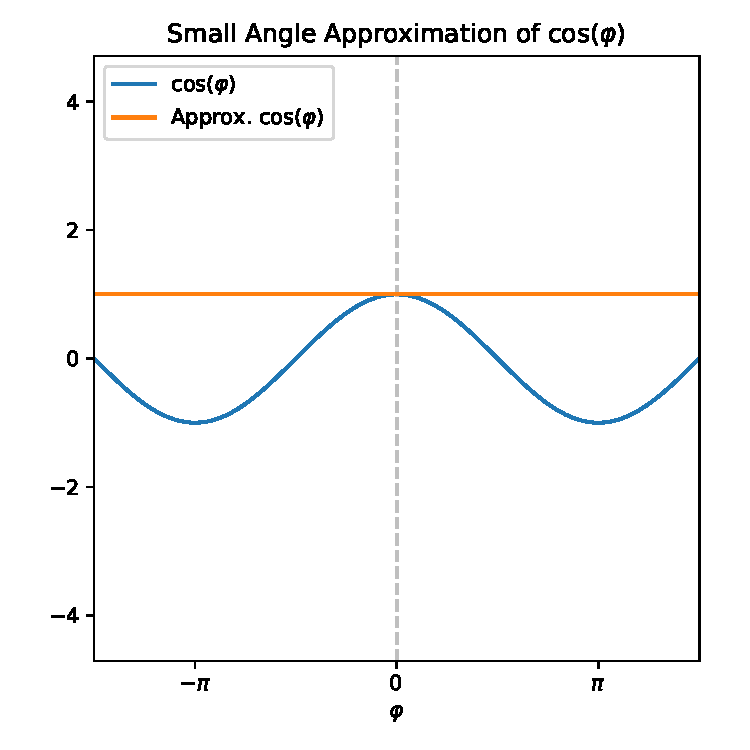
\includegraphics[width = \linewidth]{figures/introduction/generated/small-angle-approximation-cos.pdf}
			\caption{Small angle approximation \( \cos(\varphi) \approx 1 \) of Cosine.}
		\end{subfigure}
		\caption{Visualization of the small angle approximation (given in orange) of the basic trigonometric functions Sine and Cosine (given in blue). It is clear that the approximation is only valid in a small region around zero (\( \varphi \approx 0 \)).}
		\label{fig:smallAngleApproximation}
	\end{figure}

	We now look at two examples of dynamical systems, one of which is linear and one that is not.

	\paragraph{Harmonic Oscillator}
		\label{subsec:harmonicOscillator}

		\begin{figure}
			\centering
			\tikzHarmonicOscillator
			\caption{Illustration of a simple harmonic oscillator with mass \(m\), spring stiffness \(k\) and position \(x\) that is not affected by any external force like gravity. The mass is in equilibrium if \( x = 0 \).}
			\label{fig:simpleHarmonicOscillator}
		\end{figure}

		The \emph{simple harmonic oscillator} describes the dynamical system of a mass \(m\) that is attached to a spring that is following Hooke's Law with stiffness \(k\) (see~\autoref{fig:simpleHarmonicOscillator}). This harmonic oscillator is described by the \ac{ode}
		\begin{equation}
			m\ddot{x} = -kx \quad\iff\quad \ddot{x} = -\frac{k}{m} x  \label{eq:harmonicOscillator}
		\end{equation}
		where \(x\) and \(\ddot{x}\) are the position and acceleration of the mass, respectively. Note that if \( x = 0 \), the mass is in equilibrium and no force is acting on it.

		By using basic results in the solution theory of linear \acp{ode}, we see that the general solution is given as
		\begin{equation*}
			x(t) = A \cos\Big(t \sqrt{k / m} + \varphi\Big)
		\end{equation*}
		with the amplitude \(A\) and the phase \(\varphi\) (see~\autoref{app:harmonicOscillatorSolution} for the derivation of the solution). As neither gravity nor damping or other external forces are involved in the dynamical system, the motion continues forever with a non-changing amplitude.
	% end

	\paragraph{Simple Pendulum}
		\label{subsec:simplePendulum}

		\begin{figure}
			\centering
			\tikzSimplePendulum
			\caption{Illustration of an inverse pendulum with mass \(m\) and displacement \(\varphi\) that is only affected by gravity and no other external force. The mass is in equilibrium for both \( \varphi = 0 \) and \( \varphi = \pi \), where the former is an unstable equilibrium.}
			\label{fig:simplePendulum}
		\end{figure}

		The \emph{inverse pendulum} describes the dynamical system of a mass \(m\) that is attached to a rigid pole of length \(L\) which can freely swing around a suspension point (see~\autoref{fig:simplePendulum}). The pendulum stands upright if \( \varphi = 0 \) and its equation of motion is described by the \ac{ode}
		\begin{equation*}
			\ddot{\varphi} = \frac{g}{L} \sin(\varphi)
		\end{equation*}
		where \(g\), \(L\), \(\varphi\) and \(\ddot{\varphi}\) describe the gravity acceleration, pole length, displacement and acceleration of the mass, respectively. Note that if \( \varphi = 0 \), the mass is in an unstable equilibrium and no force is acting on it.

		In comparison to the harmonic oscillator (\autoref{subsec:harmonicOscillator}), this differential equation is nonlinear. And, even for the case with unit gravity acceleration \( g = 1 \) and unit pole length \( L = 1\), where the \ac{ode} looks really simple
		\begin{equation}
			\ddot{\varphi} = \sin(\varphi)  \label{eq:inversePendulum}
		\end{equation}
		it is not tractable analytically (\ie there exists no solution in closed form).

		Still, we can apply the small angle approximation introduced before (in this case, \( \sin(\varphi) \approx \varphi \)) which yields the simple \ac{ode}
		\begin{equation}
			\ddot{\varphi} \approx \varphi  \label{eq:linearizedInversePendulum}
		\end{equation}
		solved by
		\begin{equation*}
			\varphi(t) = \frac{1}{2} e^{-t} \big(\varphi_0 + e^{2t} \varphi_0 - \dot{\varphi}_0 + e^{2t} \dot{\varphi}_0\big)
		\end{equation*}
		where \(\varphi_0\) and \(\dot{\varphi}_0\) are the initial displacement and velocity, respectively.

		However, this small angle approximation can only forecast small displacements \( \varphi \ll \pi/2 \). And, as the equilibrium at \( \varphi = 0 \) is unstable, the approximation becomes worse as time goes by because the pendulum falls down. This behavior is shown in~\autoref{fig:inversePendulumApprox}.

		\begin{figure}
			\centering
			\begin{subfigure}[t]{0.5\linewidth}
				\centering
				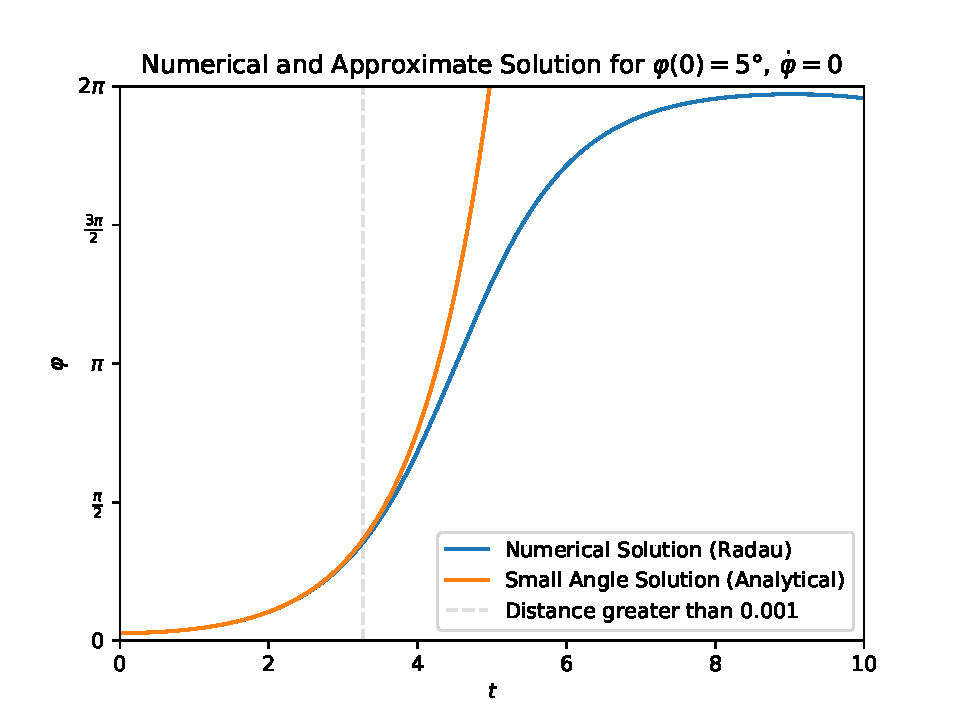
\includegraphics[width = \linewidth]{figures/introduction/generated/pendulum-motion-solutions}
				\caption{Trajectories of two solution strategies to the inverse pendulum, where the blue is a numerical solution of the actual motion of equation (solved using the Radau~IIA method~\cite[p.~72]{guglielmiImplementingRadauIIA2001}) and the orange one is the analytically computed solution linearized \ac{ode}. The latter is linearized using small angle approximation. The dashed gray vertical line shows when the distance tolerance of \( \varepsilon = 10^{-3} \) is exceeded.}
			\end{subfigure}%
			~
			\begin{subfigure}[t]{0.5\linewidth}
				\centering
				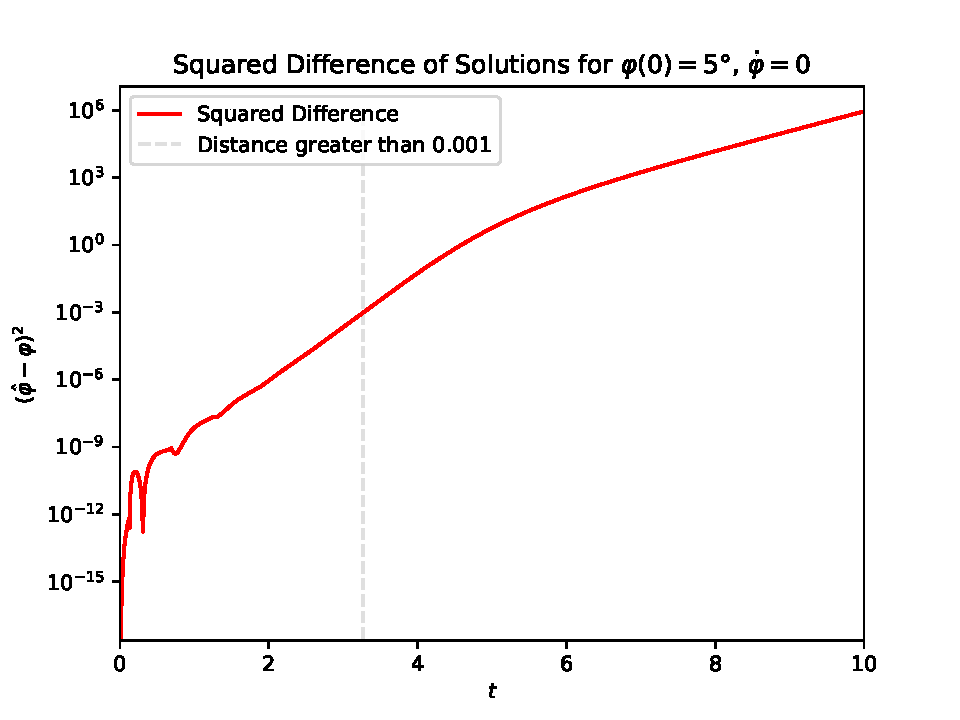
\includegraphics[width = \linewidth]{figures/introduction/generated/pendulum-motion-difference}
				\caption{Differences between the small angle approximation and the numerical solution of the \ac{ode}. The dashed gray vertical line shows when the distance tolerance of \( \varepsilon = 10^{-3} \) is exceeded.}
			\end{subfigure}
			\caption{Comparison of a numerical solution to the \ac{ode} of the inverse pendulum given in~\eqref{eq:inversePendulum} and the analytical solution of the linearized \ac{ode} given in~\eqref{eq:linearizedInversePendulum}. A tolerance value of \( \varepsilon = 10^{-3} \) is used to show when both solutions diverge from each other.}
			\label{fig:inversePendulumApprox}
		\end{figure}
	% end

	\subsection{Discrete-Time Dynamical Systems}
		In comparison to continuous-time dynamical systems described by \acp{ode}, discrete-time systems are described by a \emph{dynamics function} \( \vec{F} : \R^n \to \R^n \) advancing all states forward in time:
		\begin{equation*}
			\vec{x}_{t + 1} = \vec{F}(\vec{x}_t)
		\end{equation*}
		But we should note that, while seeming more restrictive, discrete-time dynamical systems are more general than continuous-time systems as we can discretize every continuous-time system
		\begin{equation*}
			\dot{\vec{x}} = \vec{f}(\vec{x})
		\end{equation*}
		as a discrete-time dynamical system
		\begin{equation*}
			\vec{x}_{t + 1} = \vec{F}(\vec{x}_t)
		\end{equation*}
		using the state dynamics function
		\begin{equation*}
			\vec{F}\big(\vec{x}(t_0)\big) = \vec{x}(t_0 + \Delta_t) = \vec{x}(t_0) + \int_{t_0}^{t_0 + \Delta_t} \! \vec{f}\big(\vec{x}(\tau)\big) \dd{\tau}
		\end{equation*}
		where \( \Delta_t \) is called the \emph{discretization interval} and \( \vec{x}_k = \vec{x}(k \Delta_t) \).
	% end
% end

\section{Koopman Theory of Dynamical Systems}
	Our first contribution is based on the need of a linearization technique that generalizes globally. We have seen this need in the previous chapter when looking at simple nonlinear systems and small angle approximations. This brings us directly to Koopman theory, original introduced by B.~Koopman in 1931~\cite{koopmanHamiltonianSystemsTransformation1931} in the context of Hamiltonian systems and transformations in Hilbert spaces. Considering a nonlinear discrete-time dynamical system
	\begin{equation*}
		\vec{x}_{t + 1} = \vec{F}(\vec{x}_t),\quad \vec{F} : \R^k \to \R^k
	\end{equation*}
	and observations \( \vec{h} : \R^p \to \R^p \) of this system, \ie \( \vec{y}_t \coloneqq \vec{h}(\vec{x}_t) \), the infinite-dimensional \emph{Koopman operator} \(\mathcal{K}\) advances all of the measurements forward in time. This relation can also be expressed as the composition
	\begin{equation*}
		\mathcal{K} \, \vec{h} \coloneqq \vec{h} \circ \vec{F} \qquad\iff\qquad \mathcal{K} \, \vec{h}(\vec{x}_t) = \vec{h}\big( \vec{F}(\vec{x}_t) \big) = \vec{h}(\vec{x}_{t + 1})
	\end{equation*}
	and can be visualized as a transition diagram between the states (see~\autoref{fig:koopman}). This relation is true for every possible measurement function \( \vec{h} \) at any point of the system space \( \R^k \)~\cite{bruntonKoopmanInvariantSubspaces2016}. All possible measurement functions \( \vec{h} \) span an infinite-dimensional Hilbert space \( \mathcal{H} \). A finite set of measurements \( \vec{h}_1, \vec{h}_2, \cdots, \vec{h}_p \) that span an invariant subspace \( \hat{\mathcal{H}} \subset \mathcal{H} \), \ie applying the Koopman operator to a linear combination of these functions keeps them in the subspace
	\begin{align*}
		\vec{h} &= \alpha_1 \vec{h}_1 + \alpha_2 \vec{h}_2 + \cdots + \alpha_p \vec{g}_p \\
		\mathcal{K} \, \vec{h} &= \beta_1 \vec{h}_1 + \beta_2 \vec{h}_2 + \cdots + \beta_p \vec{h}_p
	\end{align*}
	can be considered as a basis of that subspace. If that is possible, we can restrict the Koopman operator onto \( \hat{\mathcal{H}} \). Functions that both span the subspace \(\hat{\mathcal{H}}\) and do only scale when applying the Koopman operator, \ie \( \mathcal{K} \, \vec{\varphi} = \lambda \vec{\varphi} \) are called \emph{eigenfunctions} of the Koopman operator. Finding these eigenfunctions is extremely desirable, as it allows us to get a finite Koopman operator matrix \( \mat{K} \) globally linearizing the dynamical system \( \vec{F} \). However, for this thesis, we do not seek the eigenfunctions directly but an approximation of the \emph{inverse} observation function to forecast the dynamical system.

	\begin{figure}
		\centering
		\tikzKoopmanOperator
		\caption{Illustration of the transition diagram imposed by applying the Koopman operator \( \mathcal{K} \) to system dynamics \( \vec{F} \). The observation function \( \vec{h} \) is forwarded in time linearly by the Koopman operator, while the states \(\vec{x}\) are forwarded nonlinearly. The dashed lines and \( \vec{h}^{-1} \) indicate that we want to recover the original state from the linear system. \\ Adopted from~\cite{bruntonKoopmanInvariantSubspaces2016}.}
		\label{fig:koopman}
	\end{figure}
% end

\section{The Expectation-Maximization Algorithm}
	\label{sec:em}

	The \ac{em} algorithm, first introduced by Ceppellini et al. in 1955~\cite{ceppelliniEstimationGeneFrequencies1955} and popularized by Dempster et al. in 1977~\cite{dempsterMaximumLikelihoodIncomplete1977a} can be used for tackling the following problem: Assuming some model with latent (hidden) states \(\vec{x}\), observations \(\vec{y}\) and model parameters \(\vec{\theta}\), we want to maximize the likelihood \( p(\vec{y} \given \vec{\theta}) \) \ac{wrt} the latent states \(\vec{x}\) and the parameters \(\vec{\theta}\). However, the marginal distribution
	\begin{align*}
		p(\vec{y} \given \vec{\theta}) = \int\! p(\vec{x}, \vec{y} \given \vec{\theta}) \dd{\vec{x}}
	\end{align*}
	is generally intractable. As usual on maximum likelihood approaches, it is useful to not maximize the likelihood directly, but to maximize the log-likelihood
	\begin{align*}
		\mathcal{L}(\vec{\theta}) \coloneqq \log p(\vec{y} \given \vec{\theta}) = \log \int\! p(\vec{x}, \vec{y} \given \vec{\theta}) \dd{\vec{x}}
	\end{align*}
	instead. This yields the same maximum as the logarithm is strictly increasing. By introducing an auxiliary probability distribution \( q(\vec{x} \given \vec{y}) \) over the latent variables, we can rewrite the marginal and find a lower bound on \(\mathcal{L}\) by using Jensen's inequality~\cite{jensenFonctionsConvexesInegalites1906}:
	\begin{align}
		\mathcal{L}(\vec{\theta})
			&= \log \int\! p(\vec{x}, \vec{y} \given \vec{\theta}) \dd{\vec{x}}  \nonumber \\
			&= \log \int\! q(\vec{x} \given \vec{y}) \frac{p(\vec{x}, \vec{y} \given \vec{\theta})}{q(\vec{x} \given \vec{y})} \dd{\vec{x}}  \nonumber \\
			&\geq \int\! q(\vec{x} \given \vec{y}) \log \frac{p(\vec{x}, \vec{y} \given \vec{\theta})}{q(\vec{x} \given \vec{y})} \dd{\vec{x}}  \nonumber \\
			&= \int\! q(\vec{x} \given \vec{y}) \log p(\vec{x}, \vec{y} \given \vec{\theta}) \dd{\vec{x}} - \int\! q(\vec{x} \given \vec{y}) \log q(\vec{x} \given \vec{y}) \dd{\vec{x}} \eqqcolon \mathcal{L}_\mathrm{EM}[q, \vec{\theta}]  \label{eq:emLowerBound}
	\end{align}
	This draws a lower bound \( \mathcal{L}_\mathrm{EM}[q, \vec{\theta}] \) on the log-likelihood \( \mathcal{L}(\vec{\theta}) \) we can maximize instead, maximizing the log-likelihood simultaneously. Note that this lower bound is in fact a functional of the distribution \( q(\vec{x} \given \vec{y}) \).

	The \ac{em} algorithm now iteratively maximizes the lower bound and thus indirectly maximizes the original objective, the likelihood \( p(\vec{y} \given \vec{\theta}) \). The E and M step are as follows:
	\begin{description}
		\item[E-Step] Infers the auxiliary distribution \( q(\vec{x} \given \vec{y}) \) using the current estimations of the parameters \( \vec{\theta} \) by maximizing the lower bound \ac{wrt} the auxiliary distribution.
		\item[M-Step] Infers the parameters \(\vec{\theta}\) using the current auxiliary distribution by maximizing the lower bound \ac{wrt} the parameters.
	\end{description}
	Expressed in equations with the index \( \cdot^{(n)} \) to denote the values of the \(n\)-th iteration, we get the procedure which will be repeated until convergence:
	\begin{description}
		\item[E-Step] \eqparbox[r]{emSteps}{\(\displaystyle q^{(n + 1)} \)} \(\displaystyle = \arg\max_{q}\, \mathcal{L}_\mathrm{EM}\big[ q, \vec{\theta}^{(n)} \big] \)
		\item[M-Step] \eqparbox[r]{emSteps}{\(\displaystyle \vec{\theta}^{(n + 1)} \)} \(\displaystyle = \arg\max_{\vec{\theta}}\, \mathcal{L}_\mathrm{EM}\big[ q^{(n + 1)}, \vec{\theta} \big] \)
	\end{description}
	Additionally, the E-step has the constraint that \(q(\vec{x} \given \vec{y})\) really is a probability distribution, so it must integrate to one:
	\begin{align*}
		\int\! q(\vec{x} \given \vec{y}) \dd{\vec{x}} = 1
	\end{align*}
	We can incorporate this into the maximization, \eg using Lagrange multipliers. Using a bit of variational calculus, it can be shown~\cite{bealVariationalAlgorithmsApproximate2003a} that the maximization is gained by choosing the auxiliary distribution \(q(\vec{x} \given \vec{y})\) to be the same as the distribution \( p(\vec{x} \given \vec{y}, \vec{\theta}) \). That is, we set
	\begin{align*}
		q^{(n + 1)}(\vec{x} \given \vec{y}) = p\big(\vec{x} \biggiven \vec{y}, \vec{\theta}^{(n)}\big)
	\end{align*}
	while holding the parameters \(\vec{\theta}\) fixed. This maximization turns the lower bound into an equality with the actual likelihood.

	For the M-step, we keep the auxiliary distribution fixed and maximize the lower bound \ac{wrt} the parameters \(\vec{\theta}\). As this involves taking the derivative of \(\mathcal{L}_\mathrm{EM}\) \ac{wrt} \(\vec{\theta}\), we can safely omit the right hand side of the lower bound as it does not depend on \(\vec{\theta}\). Hence, we get the M-step as:
	\begin{align*}
		\vec{\theta}^{(n + 1)}
			&= \arg\max_{\vec{\theta}}\, \mathcal{L}_\mathrm{EM}\big[ q^{(n)}, \vec{\theta} \big] \\
			&= \arg\max_{\vec{\theta}} \int\! q^{(n)}(\vec{x} \given \vec{y}) \log p(\vec{x}, \vec{y} \given \vec{\theta}) \dd{\vec{x}} \\
			&= \arg\max_{\vec{\theta}} \int\! p\big(\vec{x} \biggiven \vec{y}, \vec{\theta}^{(n)}\big) \log p(\vec{x}, \vec{y} \given \vec{\theta}) \dd{\vec{x}} \\
			&= \arg\max_{\vec{\theta}}\, \E_{p\big(\vec{x} \given \vec{y}, \vec{\theta}^{(n)}\big)}[\log p(\vec{x}, \vec{y} \given \vec{\theta})]
	\end{align*}
	The quantity to optimize, \( Q(\vec{\theta}) \coloneqq \E[\log p(\vec{x}, \vec{y} \given \vec{\theta})] \), is also called the \emph{expected complete log-likelihood} as it involves both the observables and the latent variables.

	As shown in~\cite{bealVariationalAlgorithmsApproximate2003a}, the lower bound turns into an equality after the E-step. Hence we are guaranteed to always rise the log-likelihood after each \ac{em} iteration if we do not already have the optimal auxiliary distribution and parameters. If this would be the case, both the E- and the M-step would not change anything, so our log-likelihood is monotonically increasing. Also we might not want to calculate the whole distribution in the E-step, but we might want to restrict our computations to sufficient statistics that cover our whole distribution. For the rest of this thesis, we know our distribution \( p(\vec{x} \given \vec{y}, \vec{\theta}) \) is Gaussian, so we can assume the auxiliary distribution to be Gaussian too, given that we set them equal. Hence, we only need to calculate the mean and correlation or covariance of each variable to cover the whole distribution and to be able to proceed. This will turn out to be really useful later on.

	We will now take a look at variational autoencoders and justify the title of this thesis even if we, as we will see in~\autoref{c:nonlinearGaussianKoopman}, derived an \ac{em} algorithm.
% end

\section{Variational Autoencoders and the Evidence Lower Bound}
	\acp{vae} have been first introduced in the context of the \ac{aevb} algorithm by Kingma and Welling in 2014~\cite{kingmaAutoEncodingVariationalBayes2014}. They tackle inference and learning in probabilistic models with latent variables, similar to the \ac{em} algorithm. To keep the notation analogous to the derivation of the \ac{em} algorithm, we deviate from~\cite{kingmaAutoEncodingVariationalBayes2014} in terms that we keep \(\vec{x}\) as our latent variables and \(\vec{y}\) as the observables.

	To perform inference, we want to maximize the (log-) likelihood
	\begin{align*}
		\mathcal{L}(\vec{\theta}) \coloneqq \log p(\vec{y} \given \vec{\theta}) = \int\! p(\vec{x}, \vec{y} \given \vec{\theta}) \dd{\vec{x}}
	\end{align*}
	by maximizing the \ac{elbo} \( \mathcal{L}_\mathrm{ELBO} \) which we can find by using Jensen's inequality~\cite{jensenFonctionsConvexesInegalites1906}:
	\begin{align}
		\mathcal{L}(\vec{\theta})
			&= \log \int\! p(\vec{x}, \vec{y} \given \vec{\theta}) \dd{\vec{x}}  \nonumber \\
			&= \log \int\! q(\vec{x} \given \vec{y}, \vec{\phi}) \frac{p(\vec{x}, \vec{y} \given \vec{\theta})}{q(\vec{x} \given \vec{y}, \vec{\phi})} \dd{\vec{x}}  \nonumber \\
			&\geq \int\! q(\vec{x} \given \vec{y}, \vec{\phi}) \log \frac{p(\vec{x}, \vec{y} \given \vec{\theta})}{q(\vec{x} \given \vec{y}, \vec{\phi})} \dd{\vec{x}}  \nonumber \\
			&= \int\! q(\vec{x} \given \vec{y}, \vec{\phi}) \log \frac{p(\vec{y} \given \vec{x}, \vec{\theta}) p(\vec{x} \given \vec{\theta})}{q(\vec{x} \given \vec{y}, \vec{\phi})} \dd{\vec{x}}  \nonumber \\
			&= \int\! q(\vec{x} \given \vec{y}, \vec{\phi}) \frac{p(\vec{y} \given \vec{x}, \vec{\theta})}{q(\vec{x} \given \vec{y}, \vec{\phi})} \dd{\vec{x}} + \int\! q(\vec{x} \given \vec{y}, \vec{\phi}) p(\vec{y} \given \vec{x}, \vec{\theta}) \dd{\vec{x}}  \nonumber \\
			&= -\KL{q(\vec{x} \given \vec{y}, \vec{\phi})}{p(\vec{y} \given \vec{x}, \vec{\theta})} + \E_{q(\vec{x} \given \vec{y}, \vec{\phi})}[p(\vec{y} \given \vec{x}, \vec{\theta})] \eqqcolon \mathcal{L}_\mathrm{ELBO}(\vec{\theta}, \vec{\psi})  \label{eq:elbo}
	\end{align}
	Note that we have introduced an auxiliary parametric distribution \( q(\vec{x} \given \vec{y}, \vec{\phi}) \) which originally leads to the first integral to be an expectation and makes the application of Jensen's inequality possible. We now maximize the \ac{elbo}~\eqref{eq:elbo} \ac{wrt} the variational and generative parameters \(\vec{\phi}\) and \(\vec{\theta}\), respectively using the \emph{reparametrization trick}~\cite{kingmaAutoEncodingVariationalBayes2014}.

	Shifting to \acp{vae}, we now represent the auxiliary distribution \( q(\vec{x} \given \vec{y}, \vec{\phi}) \) using a neural network with some prior \( p(\vec{x} \given \vec{\theta}) \), e.g. a standard Gaussian \( p(\vec{x} \given \vec{\theta}) = \normal(\vec{0}, \mat{I}) \) to keep the latents "close to the center", enforced by the \ac{kl} divergences in the \ac{elbo}. For a Gaussian latent distribution, the neural network, called the \emph{amortization network}, produces the mean and the diagonal covariance of \( q \). A second neural network is used for decoding the latent dimension, representing the decoding distribution \( p(\vec{y} \given \vec{x}, \vec{\theta}) \). If we assume a Gaussian decoding distribution with constant variance, the right side of the \ac{elbo}~\eqref{eq:elbo} just becomes the squared error between the decoding mean and the input \(\vec{y}\). Such a network architecture is illustrated in~\autoref{fig:vae}.

	\begin{figure}
		\centering
		\tikzVariationalAutoEncoder
		\caption{Illustration of a Variational Auto-Encoder with the amortization network on the left and the decoder network on the right. Notice that the green-ish neurons in the middle are not "real", deterministic, neurons, but represent the sampling section of the \ac{vae} where the reparametrization takes place. The input and output size (on the left and right, respectively) are the same as we want to reconstruct our original data from the smaller latent state in the middle. Also the "latent neurons" are smaller than the in- and output neurons to enforce an encoding into a lower dimension.}
		\label{fig:vae}
	\end{figure}

	\subsection{Connection between EM and VAEs}
		As we have seen, the log-likelihood
		\begin{align*}
			\mathcal{L}(\vec{\theta}) = \log \int\! p(\vec{x}, \vec{y} \given \vec{\theta}) \dd{\vec{x}}
		\end{align*}
		gives rise to a lower bound \( \mathcal{L}_\mathrm{EM} \)~\eqref{eq:emLowerBound} and the \ac{elbo} \( \mathcal{L}_\mathrm{ELBO} \)~\eqref{eq:elbo}:
		\begin{gather*}
			\mathcal{L}_\mathrm{EM} = \int\! q(\vec{x} \given \vec{y}) \log p(\vec{x}, \vec{y} \given \vec{\theta}) \dd{\vec{x}} - \int\! q(\vec{x} \given \vec{y}) \log q(\vec{x} \given \vec{y}) \dd{\vec{x}} \\
			\mathcal{L}_\mathrm{ELBO} = -\KL{q(\vec{x} \given \vec{y}, \vec{\phi})}{p(\vec{y} \given \vec{x}, \vec{\theta})} + \E_{q(\vec{x} \given \vec{y}, \vec{\phi})}[p(\vec{y} \given \vec{x}, \vec{\theta})] \eqqcolon \mathcal{L}_\mathrm{ELBO}(\vec{\theta}, \vec{\psi})
		\end{gather*}
		The lower bounds look quite different, but they are in fact equivalent,
		\begin{align*}
			\mathcal{L}_\mathrm{EM} = \mathcal{L}_\mathrm{ELBO}
		\end{align*}
		as the whole difference is just that the \ac{elbo} uses a factorization \( p(\vec{x}, \vec{y} \given \vec{\theta}) = p(\vec{y} \given \vec{x}, \vec{\theta}) p(\vec{x} \given \vec{\theta}) \) and the \ac{em} lower bound does not.

		The maximization procedures differ in the following way:
		\begin{itemize}
			\item In the \ac{em} algorithm, we separately maximize the components of the lower bound, firstly finding the next auxiliary distribution \(q\) and then maximizing the lower bound \ac{wrt} the parameters.
			\item In \acp{vae}, we use an amortization network to model the auxiliary distribution \(q\) in a parameterized way. Then we maximize the lower bound \ac{wrt} to both the variational and the generative parameters at once.
		\end{itemize}
		An obvious advantage of the \ac{em} algorithm is that we are guaranteed to always rise our lower bound and we will never get worse. Also the \ac{em} algorithm requires less computation and has less parameters, depending on the model choices.
	% end
% end

	\chapter{Inference in Dynamical Systems}
\label{c:inferenceInDynamicalSystems}



Our second contribution is to take a probabilistic perspective on "classical" Koopman theory as presented in various publications~\cite{bruntonKoopmanInvariantSubspaces2016,hanDeepLearningKoopman2020,kaiserDatadrivenDiscoveryKoopman2020,luschDeepLearningUniversal2018,williamsDataDrivenApproximation2015}. In this chapter we will build the groundwork for variational inference to combine them to the single \algname algorithm presented in~\autoref{c:nonlinearGaussianKoopman}.

\section{Hidden Markov Models and LGDS}
	\acp{hmm} are simple Bayesian networks described by a non-observable (\emph{hidden}) Markov chain. This non-observable discrete chain can be indirectly observed with measurements that are emitted by every state. One of the key features of a Markov chain is that a state does only depend on the previous state, but not on the second previous, third previous, and so on, state. That is, knowing only the previous state is sufficient and no more information can be gathered by knowing every other state before. This is described by the state transition distribution
	\begin{equation*}
		s_{k + 1} \sim p(s_{k + 1} \given s_k)
	\end{equation*}
	being only dependent on the previous state \(s_k\). Analogous, a measurement \(\vec{y}_k\) of a state \(s_k\) is only dependent on that specific state:
	\begin{equation*}
		\vec{y}_k \sim p(\vec{y}_k \given s_k)
	\end{equation*}
	These assumptions are called the \emph{Markov property} and a system fulfilling this property is called \emph{Markovian}. These conditional distributions can be written in a graphical model as shown in~\autoref{fig:hiddenMarkovModel}. Note that, in general, no assumption has to be made on the "type" of state/observation (\ie whether it is a scalar, a vector or something completely different). Also, no assumption is made on the specific transition distributions, \acp{hmm} can also be used to model deterministic transitions using a Dirac delta distribution.

	\begin{figure}
		\centering
		\tikzHiddenMarkovModel
		\caption{Illustration of a completely general Hidden Markov Model with states \(s_k\) and emis\-sions/observations \(\vec{y}_k\).}
		\label{fig:hiddenMarkovModel}
	\end{figure}

	A set of closely related dynamics models are \acp{lgds} which are described by a noisy state transition
	\begin{equation*}
		\vec{s}_{t + 1} = \mat{A} \vec{s}_t + \vec{w}_t,\quad \vec{w}_t \sim \normal(\vec{0}, \mat{Q})
	\end{equation*}
	with covariance matrix \(\mat{Q}\). Similarly, the measurements \( \vec{y}_t = \mat{C} \vec{s}_t + \vec{v}_t \) underlie a Gaussian noise \( \vec{v}_t \sim \normal(\vec{0}, \mat{R}) \) too. Together they form the probabilistic model
	\begin{align*}
		\vec{s}_{t + 1} &= p(\mat{A} \vec{s}_t, \vec{Q}) \\
		\vec{y}_t &= p(\mat{C} \vec{s}_t, \mat{R})
	\end{align*}
	which fulfills the Markov property, hence the system is Markovian:
	\begin{equation*}
		p(\vec{s}_{1:T}, \vec{y}_{1:T}) = p(\vec{s}_1) \prod_{t = 2}^{T} p(\vec{s}_t \given \vec{s}_{t - 1}) \prod_{t = 1}^{T} p(\vec{y}_t \given \vec{s}_t)
	\end{equation*}
	Note that we write \( \vec{s}_{t_0:t_1} \) for the sequence \( \big( \vec{s}_{t_0}, \vec{s}_{t_0 + 1}, \rangedots, \vec{s}_{t_1} \big) \) and analogous for the observation sequence \( \vec{y}_{t_0:t_1} \). The probabilistic model of a \ac{lgds} is shown in~\autoref{fig:lgds}.

	This system is similar to a \ac{hmm} and in fact a \ac{lgds} really is an \ac{hmm}, just with continuous states \( \vec{s}_t \in \R^k \) and measurements \( \vec{y}_t \in \R^p \).

	\begin{figure}
		\centering
		\tikzLinearGaussianDynamicalSystem
		\caption{Illustration of a Linear Gaussian Dynamical System with states \(\vec{x}_t\) and observations \(\vec{y}_t\). Solid arrows represent probabilistic dependency, where the matrix \(\mat{A}\) is the dynamics matrix indicating that the mean transitions linearly, so do the observations with the observation matrix \(\mat{C}\).}
		\label{fig:lgds}
	\end{figure}
% end

\section{Inference: Filtering and Smoothing}
	\label{sec:filteringSmoothing}

	When looking at an \ac{lgds}, one of the first problems that one might consider is how to get the states (also called \emph{latent states} as we cannot observe) back? This procedure is called \emph{inference}. In this section we will give an overview on how to perform inference on an \ac{lgds}.

	For time-series data, the inference procedure is widely know as \emph{filtering} and \emph{smoothing}, where the following distributions on the latent states \( \vec{s}_t \) are calculated:
	\begin{itemize}
		\item Filtering: \tabto{2.5cm} \( p(\vec{s}_t \given \vec{y}_{1:t}) \)
		\item Smoothing: \tabto{2.5cm} \( p(\vec{s}_t \given \vec{y}_{1:T}) \)
	\end{itemize}
	That is, the filtered distribution only depends on the measurements \emph{to that time} where in contrast the smoothed distribution has used all data to the last time step \(T\) to estimate the latent states. An intermediate step in the filtering algorithm is called \emph{prediction} where the distribution \( p(\vec{s}_t \given \vec{y}_{1:t - 1}) \) is being calculated, using only the data to the previous time step. The differences between what data is used in the three steps is shown in~\autoref{fig:predictionFilteringSmoothing}.

	We will now take a look on the most used filter, the well-known \emph{Kalman Filter} and its colleague, the \emph{Rauch-Tung-Striebel Smoother}, which is also sometimes called the \emph{Kalman Smoother} as it requires a run of the Kalman filter first.

	\begin{figure}
		\centering
		\tikzPredictionFilteringSmoothing
		\caption{This diagram shows the main differences between prediction, filtering and smoothing. The shaded region describes the measurements that has been used to estimate the state at time step \(t\), indicated by a solid line. The dotted line represents time step \(t - 1\), to which all measurements are used in all three procedures. \\ Adopted from~\cite{solinCubatureIntegrationMethods2010}.}
		\label{fig:predictionFilteringSmoothing}
	\end{figure}

	\subsection{Kalman Filter}
		The Kalman filter as originally introduced by R.~Kalman in 1960~\cite{kalmanNewApproachLinear1960} in the context of signal processing to predict random signals, separate the signals from noise and detect signals of known form in the presence of noise~\cite{kalmanNewApproachLinear1960}. The normal Kalman filter assumes an underlying model of the form of an \ac{lgds} where the measurements are detected and the state is to be estimated from the data. The process of estimated the states is done in a two-step fashion:
		\begin{enumerate}
			\item Prediction: \tabto{2.5cm} Estimate the distribution \( p(\vec{s}_t \given \vec{y}_{1:t - 1}) \)
			\item Correction: \tabto{2.5cm} Estimate the distribution \( p(\vec{s}_t \given \vec{y}_{1:t}) \)
		\end{enumerate}
		For a simple linear system with Gaussian noise, \ie an \ac{lgds}, the equations for both the prediction and the correction can be given in closed form and are fairly straightforward. For the prediction step, the equations are given as
		\begin{align}
			\hat{\vec{s}}_{t \subgiven t - 1} &= \mat{A} \hat{\vec{s}}_{t - 1 \subgiven t - 1}  \label{eqn:kfStatePre} \\
			\hat{\mat{V}}_{t \subgiven t - 1} &= \mat{A} \hat{\mat{V}}_{t - 1 \subgiven t - 1} \mat{A}^T + \mat{Q}  \label{eqn:kfCovPre}
		\end{align}
		where \( \hat{\vec{s}}_{t \given t - 1} \) and \( \hat{\mat{V}}_{t \given t - 1} \) are the mean and covariance of the prediction distribution \( p(\vec{s}_t \given \vec{y}_{1:t - 1}) \), respectively. The correction step, which integrated new knowledge gained from the observation \( \vec{y}_t \) into the estimated, is given as
		\begin{align}
			\hat{\vec{s}}_{t \subgiven t} &= \hat{\vec{s}}_{t \subgiven t - 1} + \mat{K}_t \tilde{\vec{y}}_t  \label{eqn:kfStatePost} \\
			\hat{\mat{V}}_{t \subgiven t} &= \hat{\mat{V}}_{t \subgiven t - 1} - \mat{K}_t \mat{S}_t \mat{K}_t^T  \label{eqn:kfCovPost}
		\end{align}
		with the auxiliary variables
		\begin{align}
			\tilde{\vec{y}}_t &= \vec{y}_t - \mat{C} \hat{\vec{s}}_{t \subgiven t - 1}  \label{eqn:kfInno} \\
			\mat{S}_t &= \mat{C} \hat{\mat{V}}_{t \subgiven t - 1} \mat{C}^T + \mat{R}  \label{eqn:kfResCov} \\
			\mat{K}_t &= \hat{\mat{V}}_{t \subgiven t - 1} \mat{C}^T \mat{S}_t^{-1}  \label{eqn:kfKalmanGain}
		\end{align}
		known as the innovation, residual covariance and Kalman gain. The resulting estimates \( \hat{\vec{s}}_{t \subgiven t} \) and \( \hat{\mat{V}}_{t \subgiven t} \) then form the mean and covariance of the filtered distribution \( p(\vec{s}_t \given \vec{y}_{1:t}) \), respectively. These equations form a recursive algorithm "forward in time" starting off with initial state estimates \( \hat{\vec{s}}_{0 \subgiven 0} = \vec{m}_0 \) and \( \hat{\mat{V}}_{0 \subgiven 0} = \mat{V}_0 \) that have to be determined in another way.

		But these equations only work for linear systems. Lots of extensions of the regular Kalman filter have been proposed to extend the filter to nonlinear systems. The most used one is the \ac{ekf} which assumes locally linear dynamics and uses first-order Taylor expansions to linearize them. Throughout this thesis we will use the cubature Kalman filter, which we will introduce later in~\autoref{subsec:cubatureFiltering}.
	% end

	\subsection{Rauch-Tung-Striebel\,/\,Kalman Smoother}
		The \ac{rts} smoother has been introduced five years after the original Kalman filter in the 1965 by H.~E.~Rauch, F.~Tung and C.~T.~Striebel~\cite{rauchMaximumLikelihoodEstimates1965} exhibiting the equations for optimal smoothing of linear systems with Gaussian noise, \ie \ac{lgds}. With the smoother, we want to estimate the smoothed distribution, also called the \emph{posterior}
		\begin{equation*}
			p(\vec{s}_t \given \vec{y}_{1:T})
		\end{equation*}
		which uses all measurements (see again~\autoref{fig:predictionFilteringSmoothing} for an illustration). With letting the Kalman filter "run" beforehand, we have the filtered distribution \( p(\vec{s}_t \given \vec{y}_{1:t}) \) at hand. Then we have the smoothing equations as
		\begin{align}
			\hat{\vec{s}}_{t \subgiven T} &= \hat{\vec{s}}_{t \subgiven t} + \mat{J}_t (\hat{\vec{s}}_{t + 1 \subgiven T} - \hat{\vec{s}}_{t + 1 \subgiven t})  \label{eqn:rtsState} \\
			\hat{\mat{V}}_{t \subgiven T} &= \hat{\mat{V}}_{t \subgiven t} + \mat{J}_t (\hat{\mat{V}}_{t + 1 \subgiven T} - \hat{\mat{V}}_{t + 1 \subgiven t}) \mat{J}_t^T  \label{eqn:rtsCov}
		\end{align}
		with the auxiliary variable \( \mat{J}_t = \hat{\mat{V}}_{t \subgiven t} \mat{A}^T \hat{\mat{V}}_{t + 1 \subgiven t}^{-1} \). The resulting estimates \( \hat{\vec{s}}_{t \subgiven T} \) and \( \hat{\mat{V}}_{t \subgiven T} \) then form the mean and covariance of the smoothed/posterior distribution \( p(\vec{s}_t \given \vec{y}_{1:T}) \). These equations form a recursive algorithm "backward in time" starting off with the final state and covariance estimates of the filter.

		Hence, we need the Kalman filter before using the \ac{rts} smoother. Due to this hard wiring between the two algorithms, the \ac{rts} smoother is also often referred to as the Kalman smoother.

		Note that these equations only depend on the state dynamics matrix \( \mat{A} \), so a system that is linear in the state and nonlinear in the measurements can still use the standard \ac{rts} smoother and no further modification is required.
	% end
% end

\section{Cubature Rules and Filtering}
	\label{sec:cubatureRules}

	As we have already discussed, the plain Kalman filter not applicable to nonlinear systems without modifications. In this section we want to motivate the need for \emph{cubature rules} and outline their derivation and how to apply them.

	Often when deriving probabilistic algorithms like \ac{em} or the Kalman filter, we face us to evaluate expectations \( \E_{\vec{x} \sim p(\vec{x})}\big[ \vec{f}(\vec{x}) \big] \) and hence integrals of the form
	\begin{equation*}
		\E_{\vec{x} \sim p(\vec{x})}\big[ \vec{f}(\vec{x}) \big] = \int\! \vec{f}(\vec{x}) p(\vec{x}) \dd{\vec{x}}
	\end{equation*}
	In this thesis and lots of other literature, we experience Gaussian distributions \( p(\vec{x}) = \normal(\vec{x} \given \vec{\mu}, \mat{\Sigma}) \) with mean \(\vec{\mu}\) and covariance \(\mat{\Sigma}\), leading to Gaussian integrals of the form
	\begin{equation*}
		\E_{\vec{x} \sim p(\vec{x})}\big[ \vec{f}(\vec{x}) \big] = \int\! \vec{f}(\vec{x}) \, \normal(\vec{x} \given \vec{\mu}, \mat{\Sigma}) \dd{\vec{x}}
	\end{equation*}
	which do not have closed form solutions for arbitrary, nonlinear, functions \( \vec{f}(\vec{x}) \). Two common approaches for approximating the expectations/integrals are Monte Carlo Estimation, leading to particle filters and numerical integration methods, known as cubature\footnote{"Classical" numerical integration methods are called "quadrature" as they form a rectangle under the curve to approximate the area, while in higher dimensions this is more or less a "cube", hence it is called "cubature".} rules.

	To approximate Gaussian integrals, we need a set of \(m\) \emph{sigma points} \( \vec{x}_i \) to evaluate \( \vec{f}(\vec{x}) \) at and a set weights \( w_i \) to form a sum over the sigma points:
	\begin{equation*}
		\int\! \vec{f}(\vec{x}) \, \normal(\vec{x} \given \vec{\mu}, \mat{\Sigma}) \dd{\vec{x}} \approx \sum_{i = 1}^{m} w_i \vec{f}(\vec{x}_i)
	\end{equation*}
	In this thesis we utilize the spherical-radial cubature rule~\cite{solinCubatureIntegrationMethods2010} which is a third-degree approximation for Gaussian integrals. A third-degree approximation means that "this rule is exact for all monomials up to degree three"~\cite[p. 18]{solinCubatureIntegrationMethods2010}. In this cubature rule, the approximation a finite sum over \( 2n \) points, where \( n \) is the dimensionality of \(\vec{x}\), \ie \( \vec{x} \in \R^n \). With \( \mat{\Sigma}^{1/2} \) being the Cholesky decomposition of \( \mat{\Sigma} \), so \( \mat{\Sigma} = \mat{\Sigma}^{1/2} \mat{\Sigma}^{1/2, T} \), the approximation is given as
	\begin{equation*}
		\int\! \vec{f}(\vec{x}) \, \normal(\vec{x} \given \vec{\mu}, \mat{\Sigma}) \dd{\vec{x}} \approx \frac{1}{2n} \sum_{i = 1}^{2n} \vec{f}(\mat{\Sigma}^{1/2} \vec{\xi}_i - \vec{\mu})
	\end{equation*}
	with the cubature points \( \vec{\xi}_i = \sqrt{n} [\vec{1}]_i \). Here the points \( [\vec{1}]_i \) are "from the intersections between the Cartesian axes and the \(n\)-dimensional unit hypersphere"~\cite{solinCubatureIntegrationMethods2010}. That is, the point \( [\vec{1}]_i \) is the \(i\)-th row vector of the block matrix \( \begin{bmatrix} \mat{I} & -\mat{I} \end{bmatrix} \), where \( \mat{I} \) is the \(n\)-dimensional identity matrix. In the rest of this thesis we will write
	\begin{equation*}
		\SRC[\vec{f}; \vec{\mu}, \mat{\Sigma}] \coloneqq \sum_{i = 1}^{m} w_i \vec{f}(\vec{x}_i)
	\end{equation*}
	for evaluations of the spherical-radial cubature rule as it is much shorter and emphasizes the usage of the rule instead of the rule itself.

	\autoref{fig:cubature} shows the spherical-radial cubature rule working on a transition from polar coordinates to Cartesian coordinates where the transformation is given by:
	\begin{equation*}
		x = r \cos\theta \qquad\qquad y = r \sin\theta
	\end{equation*}
	The polar coordinate particles have been sampled from a multivariate Gaussian with diagonal covariance:
	\begin{equation*}
		r \sim \normal(80,\, 40) \qquad\qquad \theta \sim \normal(0,\, 0.4)
	\end{equation*}

	\begin{figure}
		\centering
		\begin{subfigure}[t]{0.5\linewidth}
			\centering
			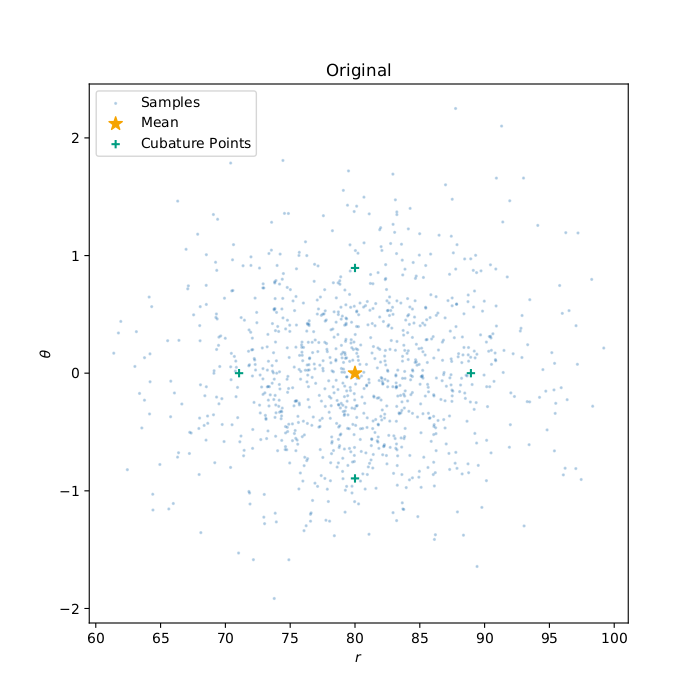
\includegraphics[width = \linewidth]{figures/inference/cubature/spherical-radial-cubature-original}
			\caption{The original samples in polar coordinates with the real mean shown as an orange star in the middle.}
		\end{subfigure}%
		~
		\begin{subfigure}[t]{0.5\linewidth}
			\centering
			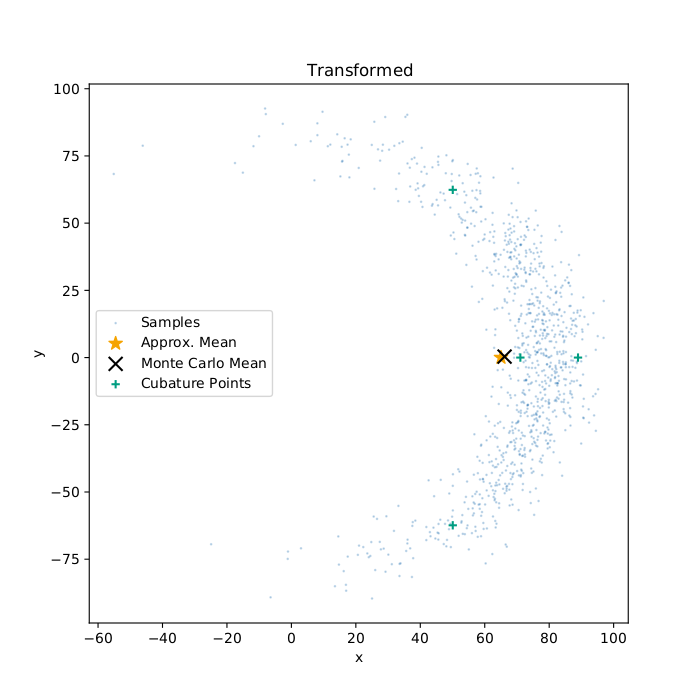
\includegraphics[width = \linewidth]{figures/inference/cubature/spherical-radial-cubature-transformed}
			\caption{The approximate mean calculated via the spherical-radial cubature rule is shown as an orange star, positioned at the mean of the transformed cubature points. This plot also shows the Monte Carlo estimate as a black cross right above the cubature estimate, showing that the cubature estimate is really accurate with significantly less computational effort.}
		\end{subfigure}
		\caption{These plots show how the spherical-radial cubature rule is used to estimate the mean of the Gaussian on the left after it has been transformed with a polar transformation to the right. To illustrate the shape of the Gaussian after it has been transformed, we added the blue dots as sample values of the Gaussian. These are 1000 sample points also used to calculate the Monte Carlo estimate of the mean. The sigma points are shown as green pluses. \\ Adopted from~\cite{solinCubatureIntegrationMethods2010}.}
		\label{fig:cubature}
	\end{figure}

	\subsection{The Unscented Transform}
		The \emph{unscented\footnote{The name "unscented", meaning "without perfume", was given by Uhlmann as he did not want people to call the corresponding filter the "Uhlmann Filter"~\cite{FirstHandUnscentedTransform}.} transform}, originally introduced by S.~J.~Julier and J.~K.~Uhlmann in 1995~\cite{julierNewApproachFiltering1995} is another method for approximating nonlinear Gaussian integrals with a parameterized transformation, the \ac{ut}. As shown by~\cite{solinCubatureIntegrationMethods2010}, the spherical-radial cubature rule is just a special case of the more general \ac{ut}. We will follow Solins derivation of this fact here. For \ac{ut}, \( 2n + 1 \) sigma points are formed as a matrix
		\begin{equation}
			\mat{\mathcal{X}} =
				\begin{bmatrix}
					\vec{\mu} & \vec{\mu} \vec{1}^T + \gamma \mat{\Sigma}^{1/2} & \vec{\mu} \vec{1}^T - \gamma \mat{\Sigma}^{1/2}
				\end{bmatrix}  \label{eqn:utSigmaPoints}
		\end{equation}
		where \( \vec{1} \) is a column vector with ones everywhere and
		\begin{equation*}
			\gamma \coloneqq \sqrt{n + \lambda} \qquad\qquad \lambda \coloneqq \alpha^2 (n + \kappa) - n
		\end{equation*}
		are a scaling parameters defined using the parameters of the \ac{ut} \( \alpha \) and \( \kappa \). The approximation for the transformed mean and covariance is then given as
		\begin{align}
			\hat{\vec{\mu}} \coloneqq \E_{\vec{x} \sim \normal(\vec{\mu}, \mat{\Sigma})}\big[ \vec{f}(\vec{x}) \big] &\approx \sum_{i = 1}^{2n + 1} w_{i - 1}^{(m)} \vec{f}(\mat{\mathcal{X}}_i)  \label{eqn:utMean} \\
			\hat{\mat{\Sigma}} \coloneqq \Cov_{\vec{x} \sim \normal(\vec{\mu}, \mat{\Sigma})}\big[ \vec{f}(\vec{x}) \big] &\approx \sum_{i = 1}^{2n + 1} w_{i - 1}^{(c)} \big( \vec{f}(\mat{\mathcal{X}}_i) - \hat{\vec{\mu}} \big) \big( \mat{\mathcal{X}}_i - \hat{\vec{\mu}} \big)^T  \label{eqn:utCov}
		\end{align}
		where \( \mat{\mathcal{X}}_i \) is the \(i\)-th column of the sigma points matrix \( \mat{\mathcal{X}} \). The weights \( w_i^{(m)} \) for the mean and \( w_i^{(c)} \) for the covariance are defined as
		\begin{align*}
			w_0^{(m)} &\coloneqq \frac{\lambda}{n + \lambda} & w_0^{(c)} &\coloneqq \frac{\lambda}{n + \lambda} + (1 - \alpha^2 + \beta) \\
			w_i^{(m)} &\coloneqq \frac{1}{2(n + \lambda)}    & w_i^{(c)} &\coloneqq \frac{1}{2(n + \lambda)}
		\end{align*}
		where \(\beta\) is another parameter of the \ac{ut}. To get back the spherical radial cubature rule, where all weights \( w_i = \flatfrac{1}(2n) \) are the same for each sigma point and the sigma point \( \mat{\mathcal{X}}_0 \) has a weight of \(0\), \ie the mean is ignored, we have to set \( \lambda = 0 \). Hence, the spherical-radial cubature rule is a special case of the \ac{ut} with the parameters set as \( \alpha = \pm 1 \), \( \beta = \kappa = 0 \). That means we can apply all theory developed for the \ac{ut} to the cubature rule by setting the parameters accordingly.
	% end

	\subsection{Cubature Kalman Filtering and Smoothing}
		\label{subsec:cubatureFiltering}

		Following~\cite{deisenrothProbabilisticPerspectiveGaussian2011,solinCubatureIntegrationMethods2010}, we can use the spherical-radial cubature rule to extend the Kalman filter and \ac{rts} smoother to nonlinear systems with Gaussian noise, \ie
		\begin{align*}
			\vec{s}_{t + 1} &\sim \normal\big( \vec{f}(\vec{s}_t), \mat{Q} \big) \\
			\vec{y}_t &\sim \normal\big( \vec{g}(\vec{s}_t), \mat{R} \big)
		\end{align*}
		In~\autoref{alg:cubatureKalmanFilter} we show the cubature Kalman filter, where the code line/equation correspondence to the linear Kalman filter is shown in~\autoref{tab:cubatureKalmanFilter}. Analogous, the cubature \ac{rts} smoother is shown in~\autoref{alg:cubatureRtsSmoother} and the correspondence table is shown in~\autoref{tab:cubatureRtsSmoother}.

		\begin{algorithm}  \DontPrintSemicolon
			\KwData{Initial state \( \vec{m}_0 \in \R^k \), covariance \( \mat{V}_0 \) and observations \( \vec{y}_{1:T} \in \R^{p \times T} \).}
			\eqmakebox[ckfinit][r]{\( \hat{\vec{s}}_{0 \subgiven 0} \gets \)} \( \vec{m}_0 \) \;
			\eqmakebox[ckfinit][r]{\( \hat{\mat{V}}_{0 \subgiven 0} \gets \)} \( \mat{V}_0 \) \;
			\For{\( t = 1, 2, \rangedots, T \)}{
				\( \vec{\xi}_i \gets \sqrt{n} [\vec{1}]_i \) \;
				\textbf{Prediction:} \;
				\quad\eqmakebox[ckf][r]{\( \vec{x}_{i, t - 1 \subgiven t - 1} \gets \)} \( \hat{\mat{V}}_{t - 1 \subgiven t - 1}^{1/2} \vec{\xi}_i + \hat{\vec{s}}_{t - 1 \subgiven t - 1} \) \;
				\quad\eqmakebox[ckf][r]{\( \hat{\vec{s}}_{t \subgiven t - 1} \gets \)} \( \frac{1}{2n} \sum_{i = 1}^{2n} \vec{f}(\vec{x}_{i, t - 1 \subgiven t - 1}) \)  \label{algline:ckfStatePre} \;
				\quad\eqmakebox[ckf][r]{\( \hat{\mat{V}}_{t \subgiven t - 1} \gets \)} \( \frac{1}{2n} \sum_{i = 1}^{2n} \vec{f}(\vec{x}_{i, t - 1 \subgiven t - 1}) \vec{f}^T(\vec{x}_{i, t - 1 \subgiven t - 1}) - \hat{\vec{s}}_{t \subgiven t - 1} \hat{\vec{s}}_{t \subgiven t - 1}^T + \mat{Q} \)  \label{algline:ckfCovPre} \;
				\textbf{Correction:} \;
				\quad\eqmakebox[ckf][r]{\( \vec{x}_{i, t \subgiven t - 1} \gets \)} \( \hat{\mat{V}}_{t \subgiven t - 1}^{1/2} + \hat{\vec{s}}_{t \subgiven t - 1} \) \;
				\quad\eqmakebox[ckf][r]{\( \hat{\vec{y}}_{t \subgiven t - 1} \gets \)} \( \frac{1}{2n} \sum_{i = 1}^{2n} \vec{g}(\vec{x}_{i, t \subgiven t - 1}) \)  \label{algline:ckfInno} \;
				\quad\eqmakebox[ckf][r]{\( \mat{S}_t \gets \)} \( \frac{1}{2n} \sum_{i = 1}^{2n} \vec{g}(\vec{x}_{i, t \subgiven t - 1}) \vec{g}^T(\vec{x}_{i, t \subgiven t - 1}) - \hat{\vec{y}}_{t \subgiven t - 1} \hat{\vec{y}}_{t \subgiven t - 1}^T + \mat{R} \)  \label{algline:ckfResCov} \;
				\quad\eqmakebox[ckf][r]{\( \mat{J}_t \gets \)} \( \frac{1}{2n} \sum_{i = 1}^{2n} \vec{f}(\vec{x}_{i, t - 1 \subgiven t - 1}) \vec{g}^T(\vec{x}_{i, t \subgiven t - 1}) - \hat{\vec{s}}_{t \subgiven t - 1} \hat{\vec{y}}_{t \subgiven t - 1}^T \) \;
				\quad\eqmakebox[ckf][r]{\( \mat{K}_t \gets \)} \( \mat{J}_t \mat{S}_t^{-1} \)  \label{algline:ckfKalmanGain} \;
				\quad\eqmakebox[ckf][r]{\( \hat{\vec{s}}_{t \subgiven t} \gets \)} \( \hat{\vec{s}}_{t \subgiven t - 1} + \mat{K}_t (\vec{y}_t - \hat{\vec{y}}_{t \subgiven t - 1}) \)  \label{algline:ckfStatePost} \;
				\quad\eqmakebox[ckf][r]{\( \hat{\mat{V}}_{t \subgiven t} \gets \)} \( \hat{\mat{V}}_{t \subgiven t - 1} + \mat{K}_t \mat{S}_t \mat{K}_t^T \)  \label{algline:ckfCovPost} \;
			}
			\caption{Spherical-Radial Cubature Kalman Filter}
			\label{alg:cubatureKalmanFilter}
		\end{algorithm}
		\begin{table}
			\centering
			\begin{tabular}{l|c|c}
				\textbf{Name}        &     \textbf{Code Line}      & \textbf{Linear Equation} \\ \hline
				Predicted State      &  \ref{algline:ckfStatePre}  &  \eqref{eqn:kfStatePre}  \\
				Predicted Covariance &   \ref{algline:ckfCovPre}   &   \eqref{eqn:kfCovPre}   \\
				Filtered State       & \ref{algline:ckfStatePost}  & \eqref{eqn:kfStatePost}  \\
				Filtered Covariance  &  \ref{algline:ckfCovPost}   &  \eqref{eqn:kfCovPost}   \\
				Innovation           &    \ref{algline:ckfInno}    &    \eqref{eqn:kfInno}    \\
				Residual Covariance  &   \ref{algline:ckfResCov}   &   \eqref{eqn:kfResCov}   \\
				Kalman Gain          & \ref{algline:ckfKalmanGain} & \eqref{eqn:kfKalmanGain}
			\end{tabular}
			\caption{This table shows how the code lines of the cubature Kalman filer relate to the corresponding linear Kalman filter equations.}
			\label{tab:cubatureKalmanFilter}
		\end{table}

		\begin{algorithm}  \DontPrintSemicolon
			\KwData{All values from the Kalman filter.}
			\For{\( t = T - 1, T - 2, \rangedots, 1 \)}{
				\eqmakebox[crts][r]{\( \vec{\xi}_i \gets \)} \(\sqrt{n} [\vec{1}]_i \) \;
				\eqmakebox[crts][r]{\( \vec{x}_i \gets \)} \( \hat{\mat{V}}_{t \subgiven t}^{1/2} \vec{\xi}_i + \hat{\vec{s}}_{t \subgiven t} \) \;
				\eqmakebox[crts][r]{\( \mat{D}_t \gets \)} \( \frac{1}{2n} \sum_{i = 1}^{2n} (\vec{x}_i - \hat{\vec{s}}_{t \subgiven t}) \big( \vec{f}(\vec{x}_i) - \hat{\vec{s}}_{t + 1 \subgiven t} \big)^T \) \;
				\eqmakebox[crts][r]{\( \mat{J}_t \gets \)} \( \mat{D}_t \hat{\mat{V}}_{t + 1 \subgiven t}^{-1} \) \;
				\eqmakebox[crts][r]{\( \hat{\vec{s}}_{t \subgiven T} \gets \)} \( \hat{\vec{s}}_{t \subgiven t} + \mat{J}_t (\hat{\vec{s}}_{t + 1 \subgiven T} - \hat{\vec{s}}_{t + 1 \subgiven t}) \)  \label{algline:crtsState} \;
				\eqmakebox[crts][r]{\( \hat{\mat{V}}_{t \subgiven T} \gets \)} \( \hat{\mat{V}}_{t \subgiven t} + \mat{J}_t (\hat{\mat{V}}_{t + 1 \subgiven T} - \hat{\mat{V}}_{t + 1 \subgiven t}) \mat{C}_t^T \)  \label{algline:crtsCov} \;
			}
			\caption{Spherical-Radial Cubature Rauch-Tung-Striebel Smoother}
			\label{alg:cubatureRtsSmoother}
		\end{algorithm}
		\begin{table}
			\centering
			\begin{tabular}{l|c|c}
				\textbf{Name}       &   \textbf{Code Line}    & \textbf{Linear Equation} \\ \hline
				Smoothed State      & \ref{algline:crtsState} &   \eqref{eqn:rtsState}   \\
				Smoothed Covariance &  \ref{algline:crtsCov}  &   \eqref{eqn:rtsState}
			\end{tabular}
			\caption{This table shows how the code lines of the cubature \ac{rts} smoother relate to the corresponding linear \ac{rts} smoother equations.}
			\label{tab:cubatureRtsSmoother}
		\end{table}
	% end

	\subsection{Square-Root Filtering\,/\,Smoothing}
		\label{subsec:sqrtSmoothing}

		While cubature rules are extremely handy, they require the Cholesky decomposition of the covariance \( \mat{\Sigma} \). The Cholesky decomposition might lead to numerical instabilities if the matrix is ill-conditioned or even not positive definite, in which case no Cholesky decomposition exists. As we will see in~\autoref{c:nonlinearGaussianKoopman}, we need the Cholesky decomposition of every smoothed covariance \( \hat{\mat{V}}_{t \subgiven T} \), \( t = 1, 2, \rangedots, T \), leading to numerical instabilities if the cubature approximation in the filtering does not "create" valid covariance matrices, \ie positive definite and symmetric matrices. One approach for solving this problem is estimating the Cholesky decomposition directly, without explicitly decomposing the matrix. Such filtering/smoothing is known as \emph{square-root filtering/smoothing}~\cite{vandermerweSquarerootUnscentedKalman2001,ruttenSquarerootUnscentedFiltering2013} and we will look into it now.

		We will mostly follow the derivation in~\cite{ruttenSquarerootUnscentedFiltering2013} and only shortly outline the key results. With the sigma points \( \mat{\mathcal{X}} \) from the \ac{ut} equation~\eqref{eqn:utSigmaPoints} and the corresponding weights, we can define the transformed sigma points
		\begin{equation*}
			\mat{\mathcal{X}}_i' = \vec{f}(\mat{\mathcal{X}}_i)
		\end{equation*}
		and utilize the \ac{ut} mean \( \hat{\vec{\mu}} \)~\eqref{eqn:utMean} and covariance \( \hat{\mat{\Sigma}} \)~\eqref{eqn:utCov} estimates. By applying another transformation to the transformed sigma points,
		\begin{equation*}
			\mat{\mathcal{Y}}_i = \sqrt{w_i^{(c)}} (\mat{\mathcal{X}}' - \hat{\vec{\mu}})
		\end{equation*}
		which are the "scaled residuals" of the sigma points, we can choose an orthogonal matrix \( \mat{\Theta} \) such that
		\begin{equation}
			\mat{\mathcal{Y}} \mat{\Theta} = \begin{bmatrix} \mat{B} & \mat{O}_{k \times (k + 1)} \end{bmatrix}  \label{eqn:sqrtFilteringQR}
		\end{equation}
		Squaring both sides of this equation yields the covariance estimate
		\begin{equation*}
			\hat{\mat{\Sigma}} = \mat{\mathcal{Y}} \mat{\mathcal{Y}}^T = \mat{\mathcal{Y}} \mat{\Theta} \mat{\Theta}^T \mat{\mathcal{Y}} = \begin{bmatrix} \mat{B} & \mat{O}_{k \times (k + 1)} \end{bmatrix} \begin{bmatrix} \mat{B}^T \\ \mat{O}_{(k + 1) \times n} \end{bmatrix} = \mat{B} \mat{B}^T
		\end{equation*}
		so \( \mat{B} \) is the Cholesky decomposition of \( \hat{\mat{\Sigma}} \). But the equation~\eqref{eqn:sqrtFilteringQR}, where we neither now the orthogonal matrix \( \mat{\Theta} \) nor the right side of the equation, is exactly the type of matrix decomposition known as the \emph{QR decomposition} that is numerically more stable than the Cholesky decomposition as it does not require any special structure like positive definiteness of the matrix. In NumPy~\cite{harrisArrayProgrammingNumPy2020}, we can easily compute the matrix \( \mat{B} \) from \( \mathbb{\mathcal{Y}} \) with
		\begin{lstlisting}
Y = np.linalg.qr(Y.T).T
		\end{lstlisting}
		By applying this argumentation in an analogous way to every covariance computation in the cubature Kalman filter and \ac{rts} smoother, we find a complete square-root filtering and smoothing algorithm propagating the Cholesky decomposition of the covariance matrices \( \hat{\mat{V}}_{t \subgiven t - 1} \), \( \hat{\mat{V}}_{t \subgiven t} \) and \( \hat{\mat{V}}_{t \subgiven T} \).

		The square-root cubature Kalman filter is summarized in~\autoref{alg:sqrtCubatureKalmanFilter} and the square-root cubature \ac{rts} smoother is summarized in~\autoref{alg:sqrtCubatureRtsSmoother}.

		The square-root filtering now allows us to pass the Cholesky decomposition of the covariances directly through the smoothing and filtering process, allowing higher numerical stability because we guarantee the covariances to be positive definite even with approximations.

		\begin{algorithm}  \DontPrintSemicolon
			\KwData{Initial state \( \vec{m}_0 \in \R^k \), covariance sqrt \( \mat{V}_0^{1/2} \) and observations \( \vec{y}_{1:T} \in \R^{p \times T} \).}
			\eqmakebox[sqrtckfinit][r]{\( \hat{\vec{s}}_{0 \subgiven 0} \gets \)} \( \vec{m}_0 \) \;
			\eqmakebox[sqrtckfinit][r]{\( \hat{\mat{V}}_{0 \subgiven 0}^{1/2} \gets \)} \( \mat{V}_0^{1/2} \) \;
			\For{\( t = 1, 2, \rangedots, T \)}{
				\eqmakebox[sqrtckf][r]{\( \mat{\Lambda} \gets \)} \( \sqrt{n} \cdot \hat{\mat{V}}_{t - 1 \subgiven t - 1}^{1/2} \) \;
				\eqmakebox[sqrtckf][r]{\( \mat{\mathcal{X}}_{t - 1 \subgiven t - 1} \gets \)} \( \begin{bmatrix} \hat{\vec{s}}_{t - 1 \subgiven t - 1} \vec{1}^T + \mat{\Lambda} & \hat{\vec{s}}_{t - 1 \subgiven t - 1} \vec{1}^T - \mat{\Lambda} \end{bmatrix} \) \;
				\eqmakebox[sqrtckf][r]{\( \mat{\mathcal{X}}_{t \subgiven t - 1, i}^s \gets \)} \( \vec{f}(\mat{\mathcal{X}}_{t - 1 \subgiven t - 1, i}) + (-1)^i \cdot \mat{Q} \),\quad \( i = 1, 2, \rangedots, 2k \) \;
				\eqmakebox[sqrtckf][r]{\( \mat{\mathcal{X}}_{t \subgiven t - 1, i}^y \gets \)} \( \vec{g}\big(\mat{\mathcal{X}}_{t \subgiven t - 1, i}^s\big) + (-1)^i \cdot \mat{R} \),\quad \( i = 1, 2, \rangedots, 2k \) \;
				\eqmakebox[sqrtckf][r]{\( \hat{\vec{s}}_{t \subgiven t - 1} \gets \)} \( \frac{1}{2k} \sum_{i = 1}^{2k} \mat{\mathcal{X}}_{t \subgiven t - 1, i}^s \) \;
				\eqmakebox[sqrtckf][r]{\( \hat{\vec{y}}_{t \subgiven t - 1} \gets \)} \( \frac{1}{2k} \sum_{i = 1}^{2k} \mat{\mathcal{X}}_{t \subgiven t - 1, i}^y \) \;
				\eqmakebox[sqrtckf][r]{\( \mat{\mathcal{Y}}_{t \subgiven t - 1, i}^s \gets \)} \( \big(\mat{\mathcal{X}}_{t \subgiven t - 1, i}^s - \hat{\vec{s}}_{t \subgiven t - 1}\big)/\sqrt{2k} \) \;
				\eqmakebox[sqrtckf][r]{\( \mat{\mathcal{Y}}_{t \subgiven t - 1, i}^y \gets \)} \( \big(\mat{\mathcal{X}}_{t \subgiven t - 1, i}^y - \hat{\vec{y}}_{t \subgiven t - 1}\big)/\sqrt{2k} \) \;
				\begin{minipage}{\linewidth}
					Find \( \mat{S}_t^{1/2} \), \( \mat{J}_t \) and \( \hat{\mat{V}}_{t \subgiven t}^{1/2} \) using the QR decomposition: \\
					\null\hspace{1cm} \(
						\begin{bmatrix}
							\mat{\mathcal{Y}}_{t \subgiven t - 1}^y \\
							\mat{\mathcal{Y}}_{t \subgiven t - 1}^s
						\end{bmatrix}
						\mat{\Theta}
						=
						\begin{bmatrix}
							\mat{S}_t^{1/2} & \mat{O} & \mat{O} \\
							\mat{J}_t       & \hat{\mat{V}}_{t \subgiven t}^{1/2} & \mat{O}
						\end{bmatrix}
					\)
				\end{minipage} \; \vspace{-0.5cm}
				\eqmakebox[sqrtckf][r]{\( \mat{K}_t \gets \)} \( \mat{J}_t \mat{S}_t^{-1/2} \) \;
				\eqmakebox[sqrtckf][r]{\( \hat{\vec{s}}_{t \subgiven t} \gets \)} \( \hat{\vec{s}}_{t \subgiven t - 1} + \mat{K}_t (\vec{y}_t - \hat{\vec{y}}_{t \subgiven t - 1}) \) \;
			}
			\caption{Square-Root Cubature Kalman Filter}
			\label{alg:sqrtCubatureKalmanFilter}
		\end{algorithm}

		\begin{algorithm}  \DontPrintSemicolon
			\KwData{All values from the Kalman filter.}
			\For{\( t = T - 1, T - 2, \rangedots, 1 \)}{
				\eqmakebox[sqrtcrts][r]{\( \mat{\mathcal{Y}}_{t \subgiven t, i}^s \gets \)} \( (\mat{\mathcal{X}}_{t \subgiven t, i} - \hat{\vec{s}}_{t \subgiven t}) \) \;
				\begin{minipage}{\linewidth}
					Find \( \mat{D}_t \) and \( \mat{Z}_t \) using the QR decomposition: \\
					\null\hspace{1cm} \(
						\begin{bmatrix}
							\mat{\mathcal{Y}}_{t + 1 \subgiven t}^s \\
							\mat{\mathcal{Y}}_{t \subgiven t}^s
						\end{bmatrix}
						\mat{\Theta}
						=
						\begin{bmatrix}
							\hat{\mat{V}}_{t + 1 \subgiven t}^{1/2} & \mat{O}   & \mat{O} \\
							\mat{D}_t                               & \mat{Z}_t & \mat{O}
						\end{bmatrix}
					\)
				\end{minipage} \; \vspace{-0.5cm}
				\eqmakebox[sqrtcrts][r]{\( \mat{J}_t \gets \)} \( \mat{D}_t \hat{\mat{V}}_{t + 1 \subgiven t}^{-1/2} \) \;
				\eqmakebox[sqrtcrts][r]{\( \hat{\vec{s}}_{t \subgiven T} \gets \)} \( \hat{\vec{s}}_{t \subgiven t} + \mat{J}_t (\hat{\vec{s}}_{t + 1 \subgiven T} - \hat{\vec{s}}_{t + 1 \subgiven t}) \) \;
				\begin{minipage}{\linewidth}
					Find \( \hat{\mat{V}}_{t \subgiven T}^{1/2} \) using the QR decomposition: \\
					\null\hspace{1cm} \(
						\begin{bmatrix}
							\mat{Z}_t & \mat{J}_t \hat{\mat{V}}_{t + 1 \subgiven T}^{1/2}
						\end{bmatrix}
						\mat{\Theta}
						=
						\begin{bmatrix}
							\hat{\mat{V}}_{t \subgiven T}^{1/2} & \mat{O}
						\end{bmatrix}
					\)
				\end{minipage} \; \vspace{-0.5cm}
			}
			\caption{Square-Root Cubature Rauch-Tung-Striebel Smoother}
			\label{alg:sqrtCubatureRtsSmoother}
		\end{algorithm}
	% end
% end

	\chapter{The Nonlinear Gaussian Koopman Algorithm}  % TODO: Find better name.
\label{c:nonlinearGaussianKoopman}
\IMRADlabel{methods}



In this chapter we will introduce out contribution and the theoretical background of the \algname algorithm that we will implement as a proof of concept in~\autoref{c:experiments}. We will start by introducing the ideas that lead to the idea, then formulate and also solve the arising (approximate) inference problem.

By looking at the graphical model for an \ac{lgds} and the state transition model for a Koopman dynamical system in~\autoref{fig:lgdsKoopmanRelation}, we can see that there are lots of similarities. The first and most interesting similarity is that both systems assume a latent state that transitions linearly, either with a state dynamics matrix \(\mat{A}\) for the \ac{lgds} or with the Koopman operator\footnote{From now on, we assume a finite-dimensional matrix approximation \(\mat{K}\) of the Koopman operator \(\mathcal{K}\).} \(\mat{K}\). The greatest difference is that measurements in classic \ac{lgds} are taken linearly with an observation matrix \( \mat{C} \) and nonlinear in the Koopman system with the measurement function \( \vec{h}(\cdot) \).

\begin{figure}
	\centering
	\begin{subfigure}[t]{0.5\linewidth}
		\centering
		\resizebox{\linewidth}{!}{\tikzLinearGaussianDynamicalSystem}
		\caption{Graphical model of a linear Gaussian dynamical system with the latent state \(\vec{s}_t\) and the (linear) observations \(\vec{y}_t\). In contrast to the Koopman system, this system is not deterministic and the arrows represent probabilistic dependency rather than hard transitions.}
	\end{subfigure}%
	\begin{subfigure}[t]{0.5\linewidth}
		\centering
		\resizebox{\linewidth}{!}{\tikzKoopmanOperator}
		\caption{State transition model of a Koopman dynamical system with the Koopman operator \( \mathcal{K} \) that can be approximated with a matrix \(\mat{K}\). In contrast to the \ac{lgds}, the state is represented via nonlinear transitions and the observations are the linear dynamics. \\ Adopted from~\cite{bruntonKoopmanInvariantSubspaces2016}.}
	\end{subfigure}
	\caption{Side-by-side comparison of the a \ac{lgds} on the left and a Koopman dynamical system on the right. This side-by-side view highlights our idea of interpreting an Koopman system as a semi-linear dynamical system (\ac{ie} an \ac{lgds} with nonlinear observations).}
	\label{fig:lgdsKoopmanRelation}
\end{figure}

Our idea is to "flip" the Koopman dynamical system and replace the observation matrix \( \mat{C} \) with a nonlinear observation function \( \vec{g}(\cdot) \), that takes the linear states \( \vec{s}_t \) and maps them into a nonlinear observation space \( \vec{y}_t \). In other words, we seek to find the inverse function of \( \vec{h}(\cdot) \) to map out of the linear embedding that Koopman theory guarantees us to exist. Our belief that such an inverse function exists is backed by previous accomplishments in data-driven Koopman analysis~\cite{luschDeepLearningUniversal2018} that also seek and find such an inverse mapping (see~\ref{c:relatedWork} for more information).

Additionally, we contribute a probabilistic view on the Koopman operator, being able to gauche our uncertainty about the embedding and the inverse mapping to the observation space. Speaking of the observation space, this is a good point to clear up chaos of notation and names that builds up when working with two systems where "observation" means contrary concepts. From now on, we will work on the graphical system shown in~\autoref{fig:nonlinearGaussianKoopman} characterized by the dynamics
\begin{align*}
	\vec{s}_{t + 1} &= \eqmakebox[ngkIntro][l]{\( \mat{A} \vec{s}_t + \vec{w}_t,\quad \vec{w}_t \)} \sim \normal(\vec{0}, \mat{Q}) \\
	\vec{y}_t       &= \eqmakebox[ngkIntro][l]{\( \vec{g}(\vec{s}_t) + \vec{v}_t,\quad \vec{v}_t \)} \sim \normal(\vec{0}, \mat{R})
\end{align*}
that can equivalently be formulated as
\begin{align*}
	\vec{s}_{t + 1} &\sim \normal(\mat{A} \vec{s}_t, \mat{Q}) \\
	\vec{y}_t       &\sim \normal\big(\vec{g}(\vec{s}_t), \mat{R}\big)
\end{align*}
We call \( \vec{s}_t \) the \emph{latent variables} or \emph{latents} in the \emph{latent space} with dimensionality \(k\), \( \vec{y}_t \) the \emph{observation variables} or \emph{observations} in the \emph{observation space} with dimensionality \(p\), \( \vec{g} : \R^k \to \R^p \) the \emph{observation function} mapping latents to observations, \( \mat{A} \) the \emph{(state) dynamics matrix}, \( \mat{Q} \) the state covariance matrix and \( \mat{R} \) the observation covariance matrix.

\begin{figure}
	\centering
	\tikzNonlinearGaussianKoopman
	\caption{The graphical model of the \algname model. Given an observation sequence \( \vec{y}_{1:T} \), we seek the latent dynamics and the corresponding nonlinear mapping \( \vec{g}(\cdot) \) from the latent space to the observations.}
	\label{fig:nonlinearGaussianKoopman}
\end{figure}

%\section{Formulating and Solving the Nonlinear Approximate Inference Problem using an Approximate EM Algorithm}
\section{Formulating and Solving the Inference Problem using an EM Algorithm}
	% Formulate likelihood, expected likelihood.
	% Shortly outline how to do the derivation and reference appendix.
	% Summarize M-step equations.
	% Combine ideas from ch. 2 (cubature and sqrt) and summarize.

	%Instead of tackling the inference problem with some kind of \ac{vae}, we choose to use an \ac{em} algorithm as it requires less training because of putting more prior knowledge and assumptions into the model, like the Gaussian noise or the specific

	We seek to find the matrices \(\mat{A}\), \(\mat{Q}\) and \(\mat{R}\) and the observation function \( \vec{g}_{\vec{\theta}}(\cdot) \), parameterized by \(\vec{\theta}\) and the initial state distribution \( \vec{s}_1 \sim \normal(\vec{m}_0, \mat{V}_0) \) that maximize the likelihood
	\begin{equation*}
		p(\vec{s}_{1:T}, \vec{y}_{1:T}) = p(\vec{s}_1) \prod_{t = 2}^{T} p(\vec{s}_t \given \vec{s}_{t - 1}) \prod_{t = 1}^{T} p(\vec{y}_t \given \vec{s}_t)
	\end{equation*}
	which factors over the conditional distributions due to the Markovian assumption. For brevity, we will keep the parameters \( \vec{\theta} \) of the observation function \( \vec{g}_{\vec{\theta}}(\cdot) \) implicit from now on. Subsequently, we can proceed by not maximizing the likelihood but the log-likelihood which is easier to maximize as the Gaussian lies in the exponential family, exhibiting a convex optimization problem\footnote{Strictly speaking, the optimization problem is only convex \ac{wrt} \(\mat{A}\) and \(\mat{Q}\). For \(\mat{R}\) and \(\vec{\theta}\), the problem is still non-convex, but numerically more stable as sums is easier to differentiate and to compute than products.}:
	\begin{equation*}
		\log p(\vec{s}_{1:T}, \vec{y}_{1:T}) = \log p(\vec{s}_1) + \sum_{t = 2}^{T} \log p(\vec{s}_t \given \vec{s}_{t - 1}) + \sum_{t = 1}^{T} \log p(\vec{y}_t \given \vec{s}_t)
	\end{equation*}
	Inserting the Gaussian distributions
	\begin{equation*}
		p(\vec{s}_1) = \normal(\vec{s}_1 \given \vec{m}_0, \mat{V}_0) \qquad\qquad
		p(\vec{s}_t \given \vec{s}_{t - 1}) = \normal(\vec{s}_t \given \mat{A} \vec{s}_{t - 1}, \mat{Q}) \qquad\qquad
		p(\vec{y}_t \given \vec{s}_t) = \normal\big(\vec{y}_t \given \vec{g}(\vec{s}_t), \mat{R}\big)
	\end{equation*}
	yields the log-likelihood
	\begin{align*}
		\log p(\vec{s}_{1:T}, \vec{y}_{1:T})
			&= -\frac{T(k + p)}{2} \log(2\pi) - \frac{1}{2} \log \lvert \mat{V}_0 \rvert - \frac{T - 1}{2} \log \lvert \mat{Q} \rvert - \frac{T}{2} \log \lvert \mat{R} \rvert \\
			&\qquad\qquad -\frac{1}{2} (\vec{s}_1 - \vec{m}_0)^T \mat{V}_0^{-1} (\vec{s}_1 - \vec{m}_0) \\
			&\qquad\qquad -\frac{1}{2} \sum_{t = 2}^{T} (\vec{s}_t - \mat{A} \vec{s}_{t - 1})^T \mat{Q}^{-1} (\vec{s}_t - \mat{A} \vec{s}_{t - 1}) \\
			&\qquad\qquad -\frac{1}{2} \sum_{t = 1}^{T} (\vec{y}_t - \vec{g}_t)^T \mat{R}^{-1} (\vec{y}_t - \vec{g}_t)
	\end{align*}
	with the abbreviation \( \vec{g}_t \coloneqq \vec{g}(\vec{s}_t) \).

	But maximizing this quantity is impossible as we do not have the latent states \( \vec{s}_{1:T} \). Hence, as usual in \ac{em} \todo{see section xy}, we instead maximize the expected log-likelihood and estimate the latent states based on out previous guess for the state dynamics. These two steps form our E- and M-step of the \algname algorithm:
	\begin{itemize}
		\item E-Step: Estimate the latent states \( \vec{s}_{1:T} \).
		\item M-Step: Maximize the expected log-likelihood \ac{wrt} the state dynamics and observation function parameters.
	\end{itemize}
	We will proceed with deriving the M-step and finish this section off by deriving the E-step. Please be aware that we only briefly touch the derivation here and focus on the important steps. See~\autoref{app:fullNgkDerivation} for the complete derivation with explanations throughout every step.

	For the M-step, we first need the expected log-likelihood \( Q \coloneqq \E_{\vec{s}_{1:T}}\big[ p(\vec{s}_{1:T}, \vec{y}_{1:T}) \big] \) as stated previously. This quantity depends on three expectations that be estimate in the E-step:
	\begin{align*}
		\hat{\vec{s}}_{t \subgiven t_0}^{(n)}  & \coloneqq \E\Big[\vec{s}_t^{(n)} \Biggiven \vec{y}_{1:t_0}\Big]                             & \hat{\vec{s}}_{t \subgiven t_0}           & \coloneqq \frac{1}{N} \sum_{n = 1}^{N} \hat{\vec{s}}_{t \subgiven t_0}^{(n)}  \\
		\mat{P}_{t \subgiven t_0}^{(n)}        & \coloneqq \E\Big[\vec{s}_t^{(n)} \vec{s}_t^{(n), T} \bigggiven \vec{y}_{1:t_0}\Big]       & \mat{P}_{t \subgiven t_0}        & \coloneqq \frac{1}{N} \sum_{n = 1}^{N} \mat{P}_{t \subgiven t_0}^{(n)}        \\
		\mat{P}_{t, t - 1 \subgiven t_0}^{(n)} & \coloneqq \E\Big[\vec{s}_t^{(n)} \vec{s}_{t - 1}^{(n), T} \bigggiven \vec{y}_{1:t_0}\Big] & \mat{P}_{t, t - 1 \subgiven t_0} & \coloneqq \frac{1}{N} \sum_{n = 1}^{N} \mat{P}_{t, t - 1 \subgiven t_0}^{(n)}
	\end{align*}
	These expectations are called the expected state, the self-correlation and the cross-correlation, respectively. We also silently introduced an upper index, \( \cdot^{(n)} \), which indicated which observation sequence our observation is from, because the algorithm can simultaneously learn on \(N\) observation sequences. For brevity, we may write \( \hat{\vec{s}}_t \) instead of \( \hat{\vec{s}}_{t \subgiven T} \) (analogous for all other values). Additionally, we have to define two quantities for the expectations of the nonlinear observation function \( \vec{g} \) that we cannot evaluate in closed form:
	\begin{align*}
		\hat{\vec{g}}_t^{(n)} &\coloneqq \E\Big[\vec{g}_t^{(n)} \Biggiven \vec{y}_{1:T}\Big] \\
		\mat{G}_t^{(n)}       &\coloneqq \E\Big[\vec{g}_t^{(n)} \vec{g}_t^{(n), T} \Biggiven \vec{y}_{1:T}\Big]
	\end{align*}
	We can now evaluate the expected log-likelihood depending on the above quantities using the trace-trick\footnote{The trace of a product of matrices/vectors is invariant under even permutations of the matrices/vectors within the trace.}, giving the following (enormous) quantity:
	\begin{align*}
		Q
			&= \E_{\vec{s}_{1:T}}\big[ p(\vec{s}_{1:T}, \vec{y}_{1:T}) \big] \\
			&= -\frac{NT(k + p)}{2} \ln(2\pi) - \frac{N}{2} \ln \lvert \mat{V}_0 \rvert - \frac{N(T - 1)}{2} \ln \lvert \mat{Q} \rvert - \frac{NT}{2} \ln \lvert \mat{R} \rvert \\
			&\qquad\qquad -\frac{N}{2} \tr\!\Big( \mat{P}_1 \mat{V}_0^{-1} \Big) + \frac{N}{2} \tr\!\Big( \hat{\vec{s}}_1 \vec{m}_0^T \mat{V}_0^{-1} \Big) + \frac{N}{2} \tr\!\Big( \vec{m}_0 \hat{\vec{s}}_1^T \mat{V}_0^{-1} \Big) - \frac{N}{2} \tr\!\Big(\vec{m}_0 \vec{m}_0^T \mat{V}_0^{-1} \Big) \\
			&\qquad\qquad -\frac{N}{2} \sum_{t = 2}^{T} \tr\!\Big( \mat{P}_t \mat{Q}^{-1} \Big) - \tr\!\Big( \mat{P}_{t, t - 1} \mat{A}^T \mat{Q}^{-1} \Big) - \tr\!\Big( \mat{A} \mat{P}_{t, t - 1} \mat{Q}^{-1} \Big) - \tr\!\Big( \mat{A} \mat{P}_{t - 1} \mat{A}^T \mat{Q}^{-1} \Big) \\
			&\qquad\qquad -\frac{1}{2} \sum_{n = 1}^{N} \sum_{t = 1}^{T} \tr\!\Big( \vec{y}_t^{(n)} \vec{y}_t^{(n), T} \mat{R}^{-1} \Big) - \tr\!\Big( \vec{y}_t^{(n)} \hat{\vec{g}}_t^{(n), T} \mat{R}^{-1} \Big) - \tr\!\Big( \hat{\vec{g}}_t^{(n)} \vec{y}_t^{(n), T} \mat{R}^{-1} \Big) + \tr\!\Big( \mat{G}_t^{(n)} \mat{R}^{-1} \Big)
	\end{align*}
	By maximizing this quantity \ac{wrt} the dynamics matrix \(\mat{A}\), the covariance matrices \(\mat{Q}\) and \(\mat{R}\), the initial state mean \(\vec{m}_0\) and the initial state covariance \(\mat{V}_0\), \ac{ie} setting the derivative \ac{wrt} these parameters to zero and rearranging the equations, we get the closed-form solutions
	\begin{align*}
		\mat{A}^\new   &= \Bigg(\! \sum_{t = 2}^{T} \mat{P}_{t, t - 1} \!\Bigg) \Bigg(\! \sum_{t = 2}^{T} \mat{P}_{t - 1} \!\Bigg)^{-1} \\
		\mat{Q}^\new   &= \frac{1}{T - 1} \Bigg(\! \sum_{t = 2}^{T} \mat{P}_t - \mat{A}^\new \sum_{t = 2}^{T} \mat{P}_{t, t - 1} \!\Bigg) \\
		\vec{m}_0^\new &= \hat{\vec{s}}_1 = \frac{1}{N} \sum_{n = 1}^{N} \hat{\vec{s}}_1^{(n)} \\
		\mat{V}_0^\new &= \mat{P}_1 - \hat{\vec{s}}_1 \hat{\vec{s}}_1^T \\
		\mat{R}^\new   &= \frac{1}{NT} \sum_{n = 1}^{N} \sum_{t = 1}^{T} \vec{y}_t^{(n)} \vec{y}_t^{(n), T} - \hat{\vec{g}}_t^{(n)} \vec{y}_t^{(n), T} - \vec{y}_t^{(n)} \hat{\vec{g}}_t^{(n), T} + \mat{G}_t^{(n), T}
	\end{align*}
	where we assume an optimal \( \vec{g}(\cdot) \) for the last equation for \(\mat{R}\). To maximize the expected log-likelihood \ac{wrt} the observation function \( \vec{g} \), we choose a learnable function approximator, \ac{eg} a neural network and maximize \(Q\) using simple gradient descent or a more evolved optimizer like Adam~\cite{kingmaAdamMethodStochastic2017}. We should note that we do not need to fully maximize \(Q\) in every M-step but that it is enough to just get better in every M-step for the convergence properties to still hold~\cite{dempsterMaximumLikelihoodIncomplete1977a}.

	We now turn to the problem of evaluating \( \hat{\vec{g}}_t^{(n)} \) and \( \mat{G}_t^{(n)} \). Instead of using Monte Carlo methods that are both very computationally expensive (especially as the gradient has to flow through the evaluation), we are employing the spherical-radial cubature rule that we have introduced in~\autoref{sec:cubatureRules}. That way, we can approximate the integrals both efficient and deterministically (as compared to Monte Carlo methods):
	\begin{align}
		\hat{\vec{g}}_t^{(n)} &= \int\! \vec{g}_t^{(n)} p\Big(\vec{s}_t^{(n)} \Biggiven \vec{y}_{1:T}\Big) \dd{\vec{s}_{1:T}^{(n)}} \approx \SRC\Big[\vec{g};\, \hat{\vec{s}}_t^{(n)}, \mat{V}_t^{(n)}\Big]  \label{eq:ngkgeval} \\
		\mat{G}_t^{(n)}       &= \int\! \vec{g}_t^{(n)} \vec{g}\vec{s}_t^{(n), T} p\Big(\vec{s}_t^{(n)} \Biggiven \vec{y}_{1:T} \Big) \dd{\vec{s}_{1:T}^{(n)}} \approx \SRC\Big[\vec{g} \vec{g}^T;\, \hat{\vec{s}}_t^{(n)}, \mat{V}_t^{(n)}\Big]  \label{eq:ngkGeval}
	\end{align}
	This concludes the derivation of the M-step, where we do not have explicit formulas for the observation parameters \(\vec{\theta}\) as we do learn these using a numerical optimizer.

	Deriving the E-step is quite straightforward given the groundwork we developed in~\autoref{sec:filteringSmoothing} and~\autoref{subsec:cubatureFiltering}. As we heavily employ cubature rules in the M-step (in fact, in every \ac{gd} iteration in the M-step), we chose to use a square-root Kalman filter and a square-root \ac{rts} smoother to directly get the Cholesky decomposition of the used covariance matrices. We apply~\autoref{alg:sqrtCubatureKalmanFilter} after afterwards~\autoref{alg:sqrtCubatureRtsSmoother} with the state dynamics function \( \vec{f} : \R^k \to \R^k : \vec{s} \mapsto \mat{A} \vec{s} \) and the observations function \( \vec{g}_{\vec{\theta}} \). Additionally to the covariances, we have to compute the self- and cross-correlation. Following~\cite{minkaHiddenMarkovModels1999}, they are given as
	\begin{align*}
		\mat{P}_t^{(n)} &= \hat{\mat{V}}_t^{(n)} - \hat{\vec{s}}_t^{(n)} \hat{\vec{s}}_t^{(n), T} \\
		\mat{P}_{t, t - 1}^{(n)} &= \hat{\mat{J}}_{t - 1} \hat{\mat{V}}_t - \hat{\vec{s}}_{t}^{(n)} \hat{\vec{s}}_{t - 1}^{(n), T}
	\end{align*}

	The whole \algname algorithm is outline in~\autoref{alg:ngk}.

	\begin{algorithm}  \DontPrintSemicolon
		\KwData{\(N\) observation sequences \( \vec{y}_{1:T}^{(n)} \in \R^{p \times T} \).}
		\textbf{Initialize} \(\mat{A}\), \(\mat{Q}\), \(\mat{R}\), \(\vec{m}_0\), \(\mat{V}_0\) and \(\vec{\theta}\) somehow (\ac{eg} identity matrices). \;
		\While{not converged}{
			\tcp{\textbf{E-Step:}}
			\( \displaystyle \vec{s}_{1:T}^{(1:N)},\, \hat{\mat{V}}_{1:T} \gets \text{\ac{rts}-Smoother} \) \;
			\eqmakebox[ngkestep][r]{\( \displaystyle \mat{P}_t^{(n)} \gets \)} \( \displaystyle \hat{\mat{V}}_t^{(n)} - \hat{\vec{s}}_t^{(n)} \hat{\vec{s}}_t^{(n), T} \) for \( t = 1, 2, \rangedots, T \) and \( n = 1, 2, \rangedots, N \) \;
			\eqmakebox[ngkestep][r]{\( \displaystyle \mat{P}_{t, t - 1}^{(n)} \gets \)} \( \displaystyle \hat{\mat{J}}_{t - 1} \hat{\mat{V}}_t - \hat{\vec{s}}_{t}^{(n)} \hat{\vec{s}}_{t - 1}^{(n), T} \) for \( t = 2, 3, \rangedots, T \) and \( n = 1, 2, \rangedots, N \) \;
			\tcp{\textbf{M-Step:}}
			\eqmakebox[ngkmstep][r]{\( \displaystyle \vec{\theta} \gets \)} \( \text{\ac{gd}}\big(Q(\vec{\theta})\big) \) \;
			\eqmakebox[ngkmstep][r]{\( \displaystyle \mat{R} \gets \)} \( \displaystyle \frac{1}{NT} \sum_{n = 1}^{N} \sum_{t = 1}^{T} \vec{y}_t^{(n)} \vec{y}_t^{(n), T} - \hat{\vec{g}}_t^{(n)} \vec{y}_t^{(n), T} - \vec{y}_t^{(n)} \hat{\vec{g}}_t^{(n), T} + \mat{G}_t^{(n), T} \) \;
			\eqmakebox[ngkmstep][r]{\( \displaystyle \mat{A} \gets \)} \( \displaystyle \Bigg(\! \sum_{t = 2}^{T} \mat{P}_{t, t - 1} \!\Bigg) \Bigg(\! \sum_{t = 2}^{T} \mat{P}_{t - 1} \!\Bigg)^{-1} \) \;
			\eqmakebox[ngkmstep][r]{\( \displaystyle \mat{Q} \gets \)} \( \displaystyle \frac{1}{T - 1} \Bigg(\! \sum_{t = 2}^{T} \mat{P}_t - \mat{A}^\new \sum_{t = 2}^{T} \mat{P}_{t, t - 1} \!\Bigg) \) \;
			\eqmakebox[ngkmstep][r]{\( \displaystyle \vec{m}_0 \gets \)} \( \displaystyle \frac{1}{N} \sum_{n = 1}^{N} \hat{\vec{s}}_1^{(n)} \) \;
			\eqmakebox[ngkmstep][r]{\( \displaystyle \mat{V}_0 \gets \)} \( \displaystyle \mat{P}_1 - \hat{\vec{s}}_1 \hat{\vec{s}}_1^T \) \;
		}
		\caption{\algname}
		\label{alg:ngk}
	\end{algorithm}
% end

\section{Implementation}
	\label{sec:implementation}

	We implemented the \algname algorithm in Python using the popular array processing library NumPy~\cite{harrisArrayProgrammingNumPy2020} throughout the whole implementation, the deep learning library PyTorch~\cite{paszkePyTorchImperativeStyle2019} for the numerical optimization of \(\vec{\theta}\) and Sacred~\cite{greffSacredInfrastructureComputational2017} for experiment management. The whole implementation can be found on GitHub\footnote{See \href{https://github.com/fdamken/bachelors-thesis_code}{\texttt{https://github.com/fdamken/bachelors-thesis\_code}}.}.

	During the implementation we focused on making the algorithm as reusable as possible, separating all data generation and investigation code from the actual implementation. Separating the data generation also has the advantage that we can run benchmarks on the exact same data to compare model performance. We have separated the optimization of \(\vec{\theta}\) as much as possible (as outlined in~\autoref{alg:ngk}) and made it possible for the user of the algorithm to easily change the optimization algorithm to use in conjunction with the parameters of the algorithm like the learning rate (defaulting to Adam~\cite{kingmaAdamMethodStochastic2017} with a learning rate of \( 0.01 \)). We also made all of the following configurable:
	\begin{itemize}
		\item Whether to perform whitening of the observation data or not. That is, if we perform whitening, we normalize and standardize the training observations beforehand using \( \hat{\vec{y}}_{1:T, i} = (\vec{y}_{1:T, i} - \bar{\vec{y}}_i) / \sigma_{y_i} \) where \( \bar{\vec{y}}_i \) is the mean and \( \sigma_{y_i} \) is the standard deviation of the \(i\)-th component of all measurements. Doing the whitening first sometimes improves the performance as we will see in~\ref{c:experiments}.
		\item The convergence precision, \ac{ie} how much the log-likelihood has to change in order to continue the \ac{em} iterations. We will see that, due to numerical instabilities and approximation errors in the cubature rules, the algorithm rarely really converges before becoming numerically unstable.
		\item That is why we also made the maximum number of iterations configurable to support \emph{early stopping}. Once the algorithm performed these number of \ac{em} iterations, it will abort and report the results.
		\item Similarly it is possible to configure the convergence precision and maximum number of iterations for the subsequent optimization of \(\vec{\theta}\).
	\end{itemize}
	These are only the parameters that can be configured directly on the \ac{em} algorithm, but the user is also able to specify how to initialize everything, \ac{ie} the matrices \( \mat{A} \), \( \mat{Q} \), \( \mat{R} \), \( \mat{V}_0 \), \( \vec{m}_0 \) and the parameters \( \vec{\theta} \) of the observation function \( \vec{g}_{\vec{\theta}} \). Speaking of the observation function, we used a neural network with \( \tanh \) activation function and a single hidden layer for all experiments (see~\autoref{c:experiments} for more information about the experiment setup). We made it also possible to pass arbitrary Torch modules as the function approximator that can be learned via a \ac{gd}-like algorithm (\ac{ie} they must be differentiable and expose parameters).

	For learning multiple observation sequences, as outlined in the derivation of the \algname algorithm in~\autoref{c:nonlinearGaussianKoopman}, it turns out to be useful to add noise to the training data which has the effect of regularizing the algorithm a bit. This effect is visible in smoother log-likelihood curves as we will see in~\autoref{c:experiments}.

	\subsection{Insights, Problems and Solutions}
		In this section we will focus on interesting insights and problems we found during the implementation and how to (possibly) solve them.

		\subsubsection{Slow QR Decomposition on GPU}
			During our implementation we found found that QR decomposition is relatively slow on the \ac{gpu} due to a bug in PyTorch\footnote{See \href{https://web.archive.org/web/20201110121407/https://github.com/pytorch/pytorch/issues/22573}{\texttt{https://github.com/pytorch/pytorch/issues/22573}}.} at the time of writing. While faster QR decomposition methods on a \ac{gpu} have been proposed~\cite{andersonCommunicationAvoidingQRDecomposition2011a}, we stuck to copying the data back and forth between \ac{cpu} and \ac{gpu} in every \ac{em} iteration.
		% end

		\subsubsection{Diagonal Covariance}
			As we assumed the noise to be independent\todo{Include that assumption in the theoretical section!}, we can safely omit the non-diagonal entries of the covariance \( \mat{Q} \), \( \mat{R} \) and \( \mat{V}_0 \). That way we further reduce the computational overhead that would other wise be generated as we still (even with square-root filtering) have to compute the Cholesky decomposition of \( \mat{Q} \) and \( \mat{R} \). We can now just take the square-root of the diagonal entries and get the Cholesky decomposition around ten times faster\todo{Cite something or add experiment?}.

			% >>> As = [np.diag(np.random.random(size=(1000,)) ** 2) for n in range(1000)]
			% >>> timeit.timeit(lambda: [np.linalg.cholesky(A) for A in As], number=10)
			% 50.62359843800368
			% >>> timeit.timeit(lambda: [np.diag(np.sqrt(np.diag(A))) for A in As], number=10)
			% 4.582914652011823
			% >>> 50.62359843800368 / 4.582914652011823
			% 11.046157801734486
		% end

		\subsubsection{Regularization and Learning Cholesky Decompositions}
			There are also a few points where our code is extensible to make it faster, improve numerical stability and so on (see also~\autoref{sec:futureWork}). The main points are regularization and/or learning the Cholesky decomposition directly.

			As we will see in~\autoref{c:experiments}, having singular and non-positive definite matrices is a big problem that should be assessed. We already implemented the square-root smoothing that increased the numerical stability through the smoothing by not allowing non-positive definite matrices to be produced by the smoothing at all (as we directly learn the Cholesky decomposition). Additional regularization might make sense at the computation of the covariance matrices \(\mat{Q}\), \(\mat{R}\) and \(\mat{V}_0\). Another approach would be to learn the Cholesky decomposition of the covariance matrices \(\mat{Q}\), \(\mat{R}\) and \(\mat{V}_0\) directly by replacing the explicit formulas with a \ac{gd} algorithm that directly learn the Cholesky or the square-root diagonal. As the optimization problem is still convex\todo{This is a hot take.}, finding the global optimum should be easily possible.

			However we sadly did not have more time to look into this idea.
		% end
	% end

	\subsection{Hyperparameters}
		One of the largest hyperparameter with high influence is obviously the architectural choice for \( \vec{g}_{\vec{\theta}} \). As it turns out, even simple models like a single hidden layer produce good results as we will see in~\autoref{c:experiments} and~\autoref{c:discussion}. A \( \tanh \) activation function turns out to be really suitable as it produces smooth results compared to \ac{eg} a step function or \ac{relu}. The other high-influence hyperparameter is the dimensionality \(k\) of the latent space, \ac{ie} how many dimensions the Koopman operator has to build up a linear system that, taking the observations, behaves the same as the original nonlinear system. We will further investigate into the dependence on this hyperparameter in~\autoref{subsec:experimentLatentDim}.

		On the same page is the maximum number of iterations in the numerical optimization of \( \vec{\theta} \). High maximum iterations seem to lead to overfitting on the neural network, causing the whole algorithm to not generalize well. On the other hand, too less iterations do not raise the likelihood enough to get reasonable results.
	% end
% end

	\chapter{Experiments}
\label{c:experiments}
\IMRADlabel{results}



In this chapter we will present all environments we experimented with as well as \emph{hyper-experiments}, \ie experiments with the hyperparameters and their influence on the algorithm performance (in terms of the prediction error and similar metrics, not the computing time).

We split this chapter into two parts: Firstly, we will present the experiment setup we used and the different environments we tested on. Secondly, we present our results and put them in context of other results. All critical discussion and comparison with related work will take place in~\autoref{c:discussion}.

\section{Setup}
	In this section we will introduce the experiment setup and all the different environments we used for evaluation.

	\subsection{Environments}
		This section covers the different environments we used and changes we have applied to them. Note that we separated the data generation process from running the experiment. For each of the following experiments we include the experiment ID at the beginning that can be used to locate the experiment in the code.

		\subsubsection{Proof-of-Concept: Classic LGDS}
			\begin{itemize}
				\item Experiment ID: \texttt{lgds}
			\end{itemize}

			As a proof-of-concept and to empirically verify our proof on the exactness of the cubature rule and hence the similar expected performance for plain linear systems, we benchmark our algorithm against a simple linear system. The linear system has a two-dimensional state \( \vec{y} \coloneqq \begin{bmatrix} x_1 & x_2 \end{bmatrix}^T \) with the dynamics
			\begin{align*}
				\dot{x}_1 &= x_2 \\
				\dot{x}_2 &= -x_1
			\end{align*}
			The initial state \( \vec{s}_1 \) is sampled from a Gaussian with mean \( \begin{bmatrix} 0.1 & 0.2 \end{bmatrix}^T \) and covariance \( \diag\big(10^{-5}, 10^{-5}\big) \). The system is integrated using the implicit Runge-Kutta Radau~IIA~\cite{guglielmiImplementingRadauIIA2001} method with an evaluation interval of \( h = 0.1 \) for \( T = 240 \) time steps where only the first \( T_\train = 120 \) steps are used for training and the remaining \(120\) are used for validation. The raw data is shown in~\autoref{fig:envLgds}.

			As the system's eigenvalues \( -i \), \( i \) are purely imaginary, the integrated system rings around the equilibrium \( \begin{bmatrix} 0 & 0 \end{bmatrix}^T \) indefinitely.

			\begin{figure}
				\centering
				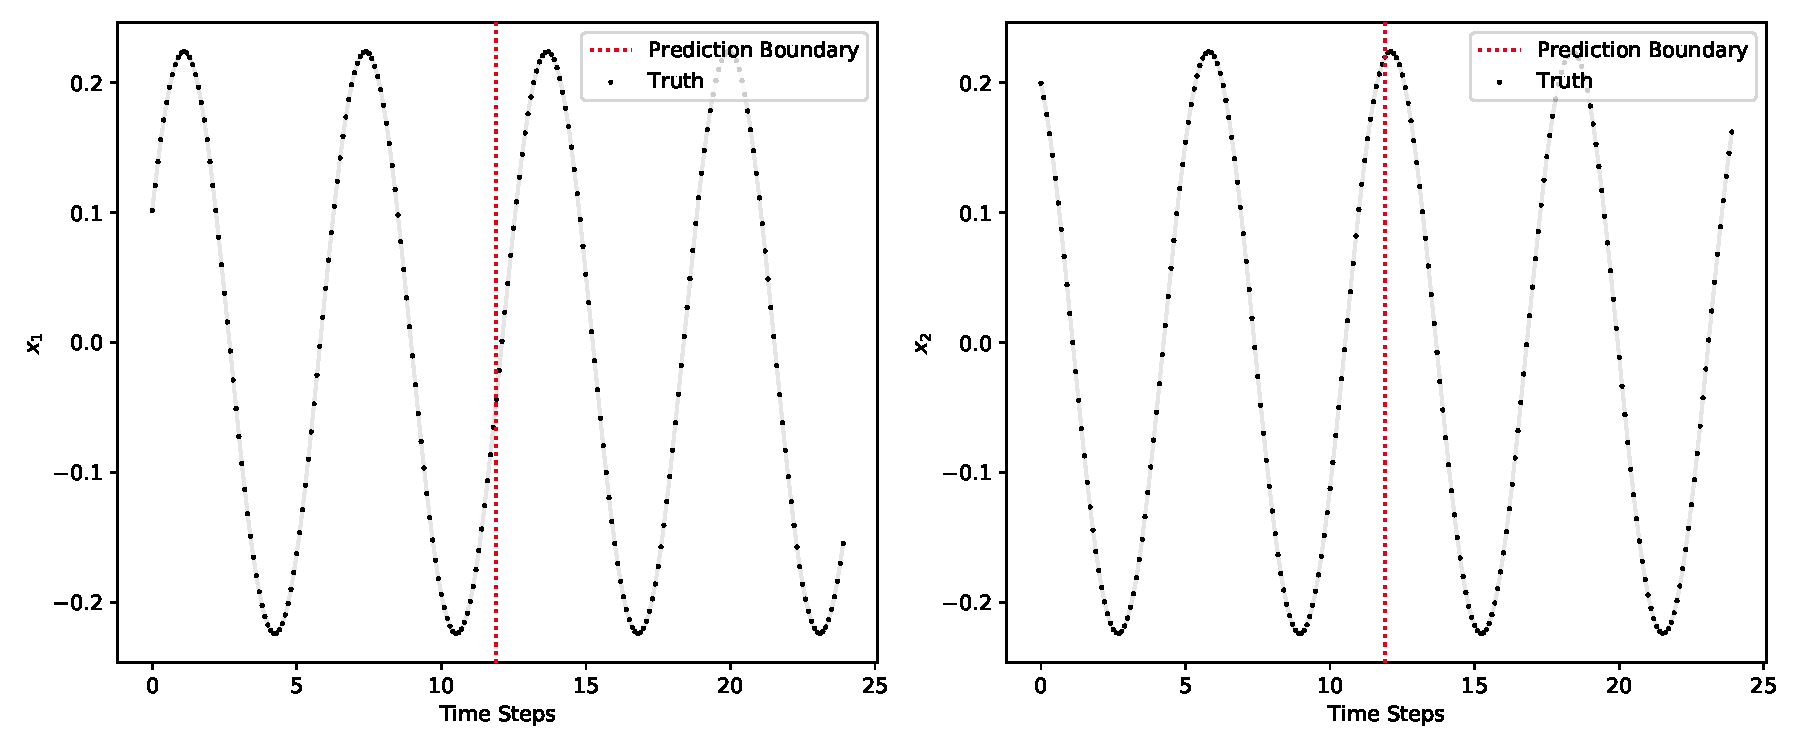
\includegraphics[width=\linewidth]{figures/experiments/environments/observations-lgds-N0.png}
				\caption[Raw data of the proof-of-concept LGDS environment]{Plot of the raw data used for training the proof-of-concept LGDS environment with the first dimension on the left and the second dimension on the right. The black dots represent the actual data points, all before the red prediction boundary are used for training, the rest for validation. The faint gray line emphasizes the connection between the data points and that they are actually generated from a dynamical system.}
				\label{fig:envLgds}
			\end{figure}
		% end

		\subsubsection{(Damped) Pendulum}
			\begin{itemize}
				\item Experiment ID: \texttt{pendulum} and \texttt{pendulum\_damped}
			\end{itemize}

			The first nonlinear system we look at is the (inverted) pendulum in both an undamped and a damped setting. For this experiment, we use the angular state \( \vec{y} = \begin{bmatrix} \theta & \dot{\theta} \end{bmatrix} \) where \(\theta\) is the displacement angle (see~\autoref{fig:envPendulumSketch}). The dynamics are specified by the \ac{ode}
			\begin{equation*}
				\ddot{\theta} = \sin\theta - d \dot{\theta}
			\end{equation*}
			that is solved using the Radau~IIA~\cite{guglielmiImplementingRadauIIA2001} \ac{ivp} integrator (after transforming the \ac{ode} to a first-order \ac{ode} system). The initial velocity is set to \(0\) and the initial position is sampled from a Gaussian with mean \( \pi/36 \) and variance \( \pi/8 \). This puts the pendulum in motion as it falls down from its initial position. For the undamped pendulum, we set \( d = 0 \). For both environments, we use an evaluation interval of \( h = 0.1 \) for \( T = 1000 \) time steps where only the first \( T_\train = 500 \) steps are used for training and the remaining \(500\) are used for validation. The raw data is shown in~\autoref{fig:envPendulum} for the undamped and~\autoref{fig:envPendulumDamped} for the damped pendulum.

			The damped pendulum is especially interesting as the system looses energy (\ie the sum of the kinetic and potential energy decreases over time) and the embedding has to encode this behavior.

			\begin{figure}
				\centering
				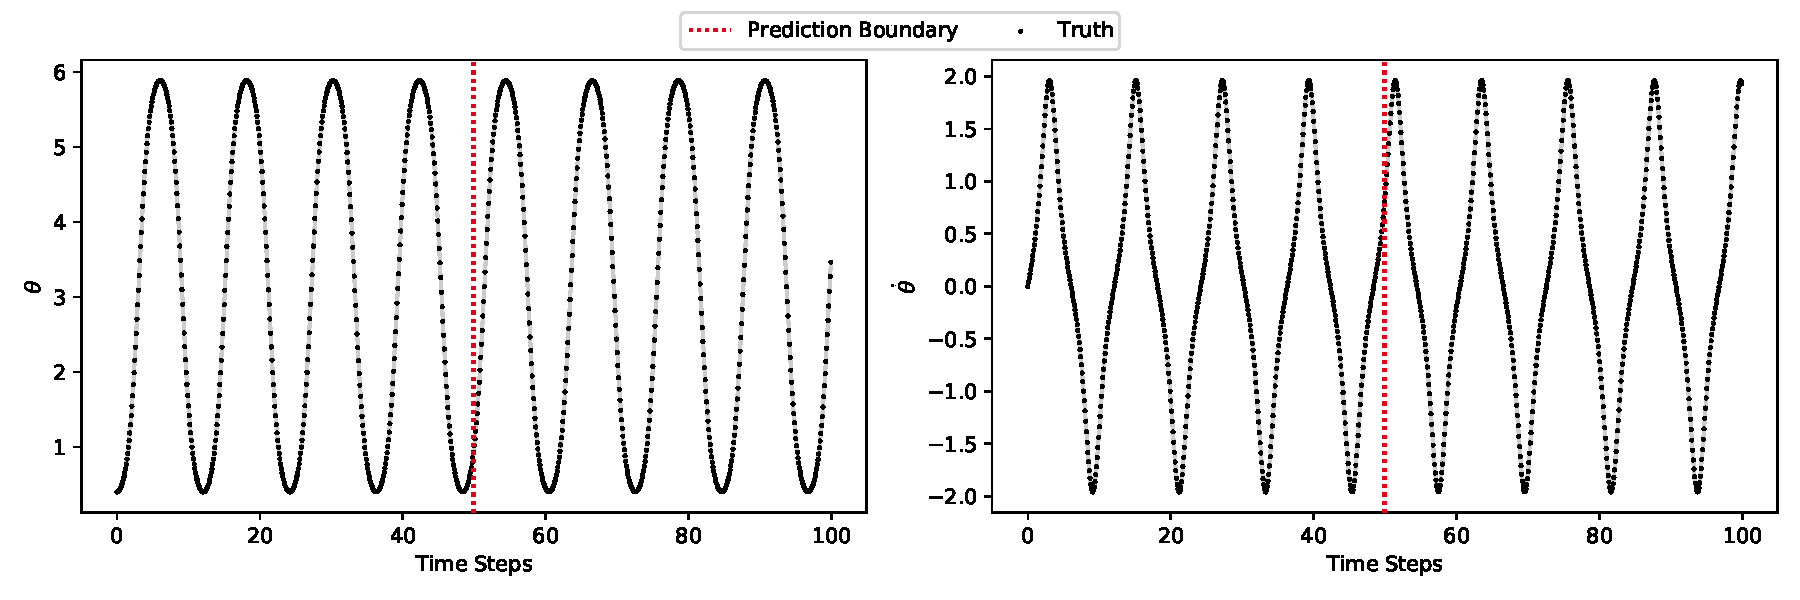
\includegraphics[width=\linewidth]{figures/experiments/environments/observations-pendulum-N0.png}
				\caption[Raw data of the undamped pendulum environment]{Plot of the raw data used for training the undamped pendulum environment. The left plot shows the displacement and the right plot the angular velocity. The black dots represent the actual data points, all before the red prediction boundary are used for training, the rest for validation. The faint gray line emphasizes the connection between the data points and that they are actually generated from a dynamical system.}
				\label{fig:envPendulum}
			\end{figure}
			\begin{figure}
				\centering
				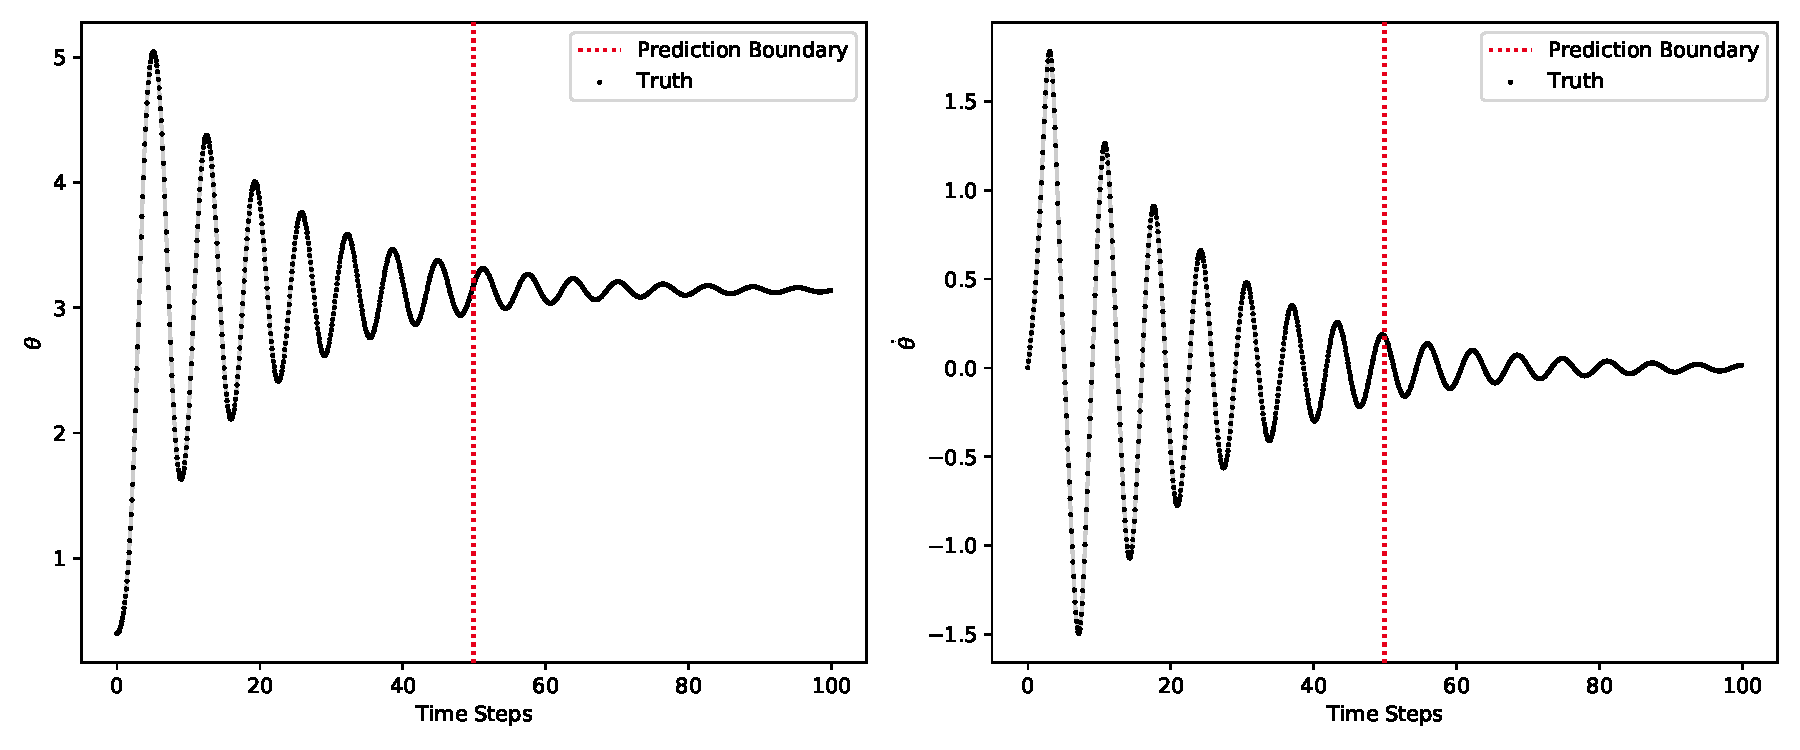
\includegraphics[width=\linewidth]{figures/experiments/environments/observations-pendulum-damped-N0.png}
				\caption[Raw data of the damped pendulum environment]{Plot of the raw data used for training the damped pendulum environment. The left plot shows the displacement and the right plot the angular velocity. The black dots represent the actual data points, all before the red prediction boundary are used for training, the rest for validation. The faint gray line emphasizes the connection between the data points and that they are actually generated from a dynamical system.}
				\label{fig:envPendulumDamped}
			\end{figure}

			\begin{figure}
				\centering
				\tikzSimplePendulum
				\caption[Illustration of the pendulum environment]{Illustration of the pendulum environment. The pendulum has length \(L\) and mass \(m\) and is attached to a fixed point in the center around which it can swing. In the case of the damped pendulum is damped with a damping constant \(d\).}
				\label{fig:envPendulumSketch}
			\end{figure}
		% end

		\subsubsection{Gym Pendulum}
			\begin{itemize}
				\item Experiment ID: \texttt{pendulum\_gym}
			\end{itemize}

			This is a sine/cosine version of the pendulum introduced before, but without damping. We use the environment of OpenAI Gym~\cite{brockmanOpenAIGym2016} for generating the data used for training. The motion equations are still the same as for the non-Gym pendulum
			\begin{equation*}
				\ddot{\theta} = \sin\theta
			\end{equation*}
			with \( d = 0 \) as the Gym pendulum does not include damping, but the state is defined as the sine and cosine of the angle:
			\begin{equation*}
				\vec{y} \coloneqq
					\begin{bmatrix}
						\cos\theta \\
						\sin\theta \\
						\dot{\theta}
					\end{bmatrix}
			\end{equation*}
			The Gym environment uses the Euler method for integrating the \ac{ode} with a step size of \( h = 0.05 \). We generate \( T = 100 \) time steps of which \( T_\train = 50 \) are used for training and the other \(50\) for validation. The raw data is shown in~\autoref{fig:envPendulumGym}.

			\begin{figure}
				\centering
				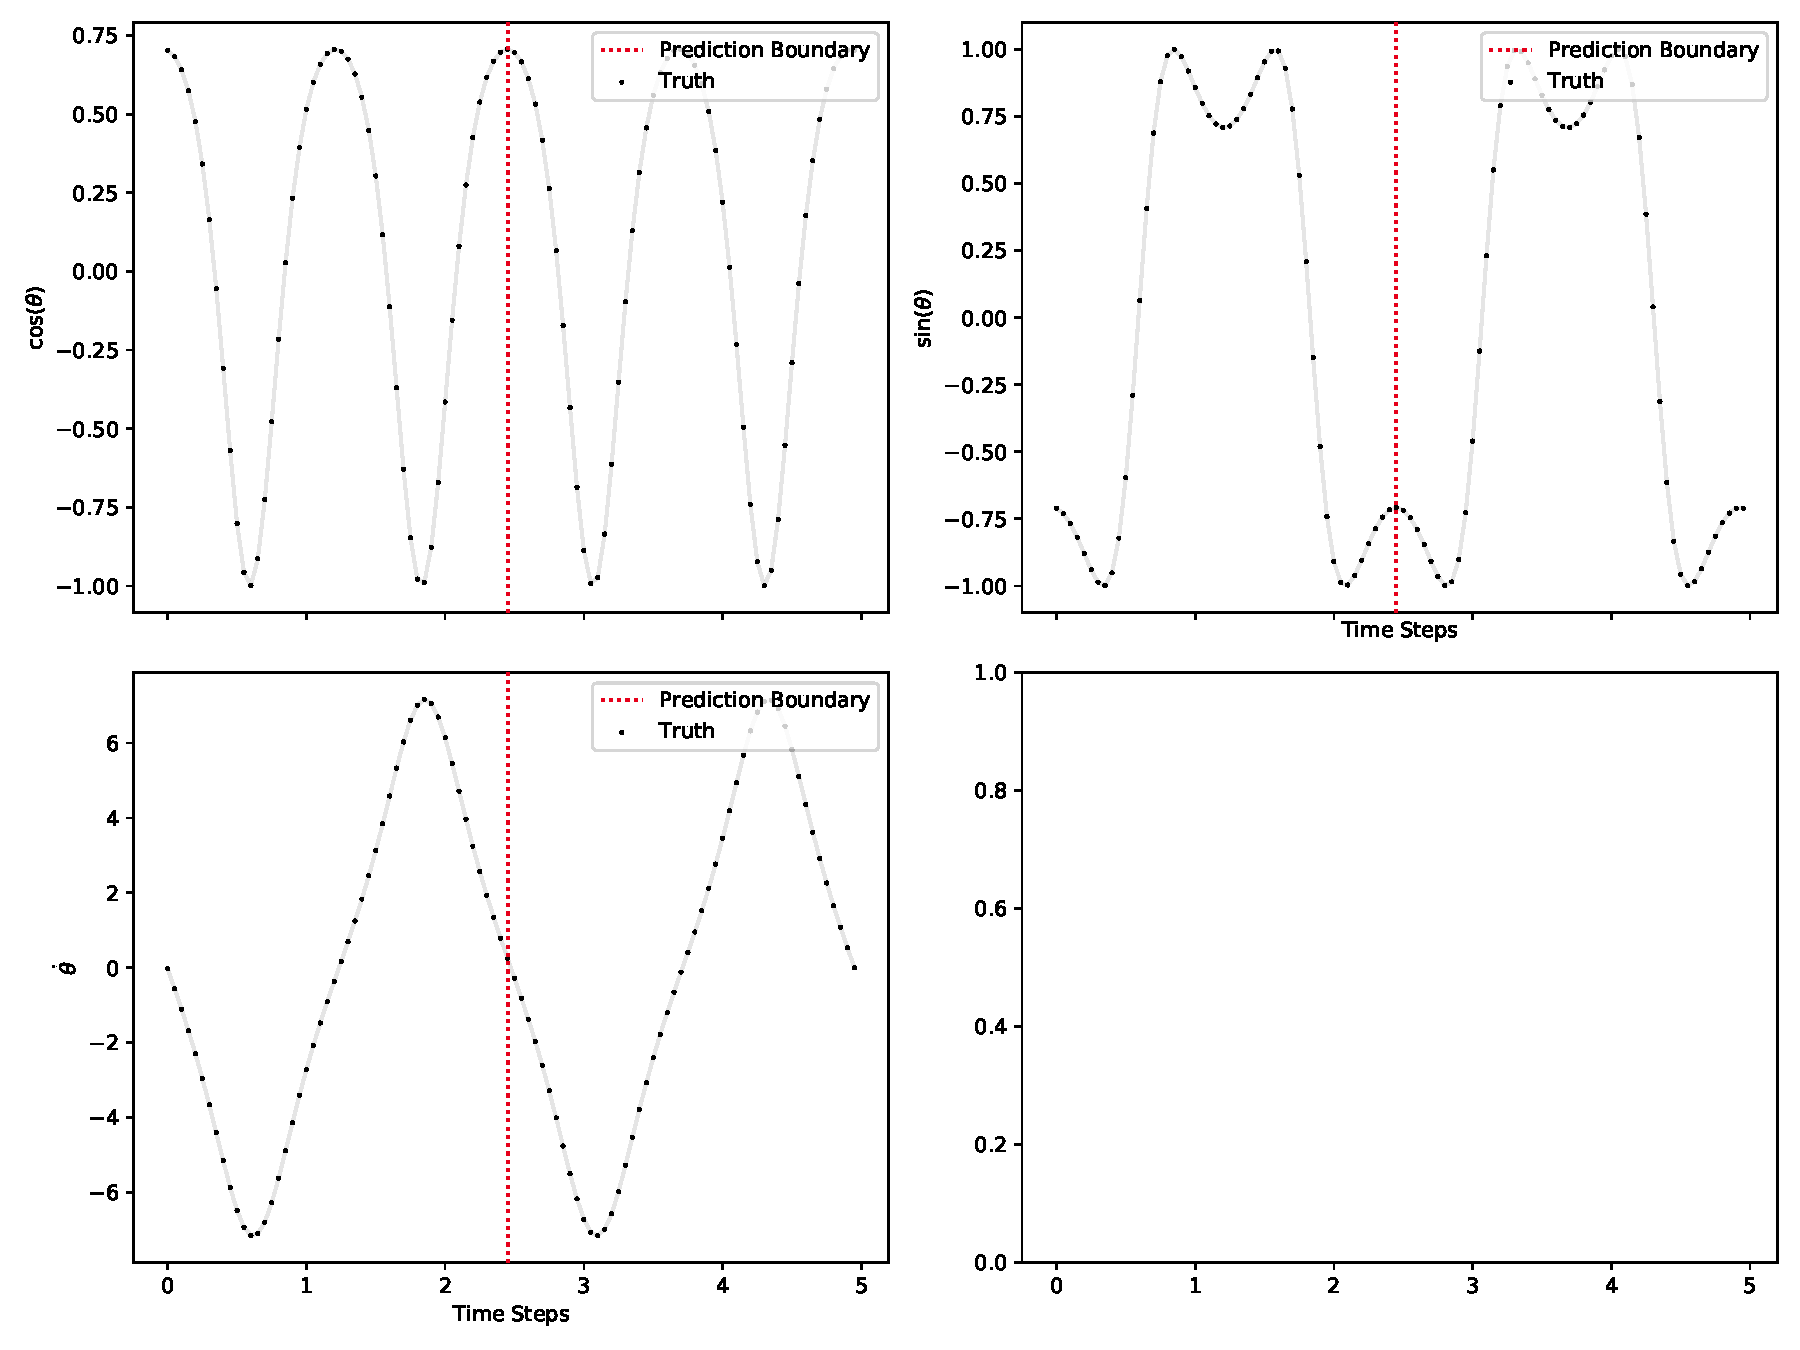
\includegraphics[width=\linewidth]{figures/experiments/environments/observations-pendulum-gym-N0.png}
				\caption[Raw data of the Gym pendulum environment]{Plot of the raw data used for training the Gym pendulum environment. The top row shows the cosine/sine of the displacement of the pendulum and the bottom plot shows the angular velocity. The black dots represent the actual data points, all before the red prediction boundary are used for training, the rest for validation. The faint gray line emphasizes the connection between the data points and that they are actually generated from a dynamical system.}
				\label{fig:envPendulumGym}
			\end{figure}
		% end

		\subsubsection{Gym Cartpole}
			\label{subsubsec:cartpole}

			\begin{itemize}
				\item Experiment ID: \texttt{cartpole\_gym}
			\end{itemize}

			The second last environment we run experiment on is the cartpole environment. In the cartpole environment, an inverted pendulum is build on a (typically controlled, but otherwise freely movable) cart. If the pendulum falls down, the torque on the joint is translated into a force moving the cart around. This creates nonlinear coupling and therefore, highly nonlinear dynamics. A sketch of the cartpole environment is given in~\autoref{fig:envCartpoleGymSketch}. As for the previous pendulum, we rely on the cartpole implementation of Gym. We slightly modified the environment to be uncontrolled, as the environment usually has discrete actions for pushing the cart left or right. This modification is shown in~\autoref{lst:uncontrolledCartPole}. The state of the environment is given as
			\begin{equation*}
				\vec{y} \coloneqq
					\begin{bmatrix}
						x \\
						\dot{x} \\
						\theta \\
						\dot{\theta}
					\end{bmatrix}
			\end{equation*}
			where \(x\) is the cart position, \(\dot{x}\) is the cart velocity, \(\theta\) is the pole angle and \(\dot{\theta}\) is the angular velocity. The implemented equations of movement, taken from~\cite{florianCorrectEquationsDynamics2005}, are given as:
			\begin{align*}
				\ddot{\theta} &= \frac{g \sin\theta + \cos\theta \Big(\! \frac{-F - m_p \ell \dot{\theta}^2 \sin\theta}{m_c + m_p} \!\Big)}{\ell \Big(\! \frac{4}{3} - \frac{m_p \cos^2\theta}{m_c + m_p} \!\Big)} \\
				\ddot{x} &= \frac{F + m_p \ell \big( \dot{\theta}^2 \sin\theta - \ddot{\theta} \cos\theta \big)}{m_c + m_p}
			\end{align*}
			Here \( g = \SI{9.8}{\meter\per\second\squared} \) is the gravitational acceleration, \( m_p = \SI{0.1}{\kilogram} \) and \( m_c = \SI{1}{\kilogram} \) are the masses of the pole and cart, respectively, \( 2\ell = \SI{1}{\meter} \) is the pole length and \( [F] = \si{\newton} \) is the external (control) force acting on the cart that we set to \( \SI{0}{\newton} \). The Gym environment uses an implicit Euler method\footnote{As mentioned in~\autoref{subsubsec:integrationProblems}, this has to be set manually with \lstinline|env.kinematics_integrator = 'implicit-euler'|.} for integrating the \ac{ode} with a step size of \( h = 0.02 \). We generate \( T = 300 \) time steps of which we use \( T_\train = 150 \) for training and the remaining \(150\) steps for validation. The raw data is shown in~\autoref{fig:envCartpoleGym}.

			\begin{lstlisting}[caption={[Modification of Gym's cartpole environment to get an uncontrolled cartpole]Modification of Gym's cartpole environment to get an uncontrolled cartpole.}, label=lst:uncontrolledCartPole]
from gym.envs.classic_control import CartPoleEnv

class UncontrolledCartPole(CartPoleEnv):
	def __init__(self):
	super().__init__()

	self.force_mag = 0.0
			\end{lstlisting}

			\begin{figure}
				\centering
				\tikzCartpole
				\caption[Illustration of the cartpole environment]{Illustration of the cartpole environment. The cart has mass \(m_c\), the pole \(m_p\) with length \(L\). The cart can move freely on the \(x\) axis, while the pendulum can swing freely around the center of the cart, causing the cart to move.}
				\label{fig:envCartpoleGymSketch}
			\end{figure}

			\begin{figure}
				\centering
				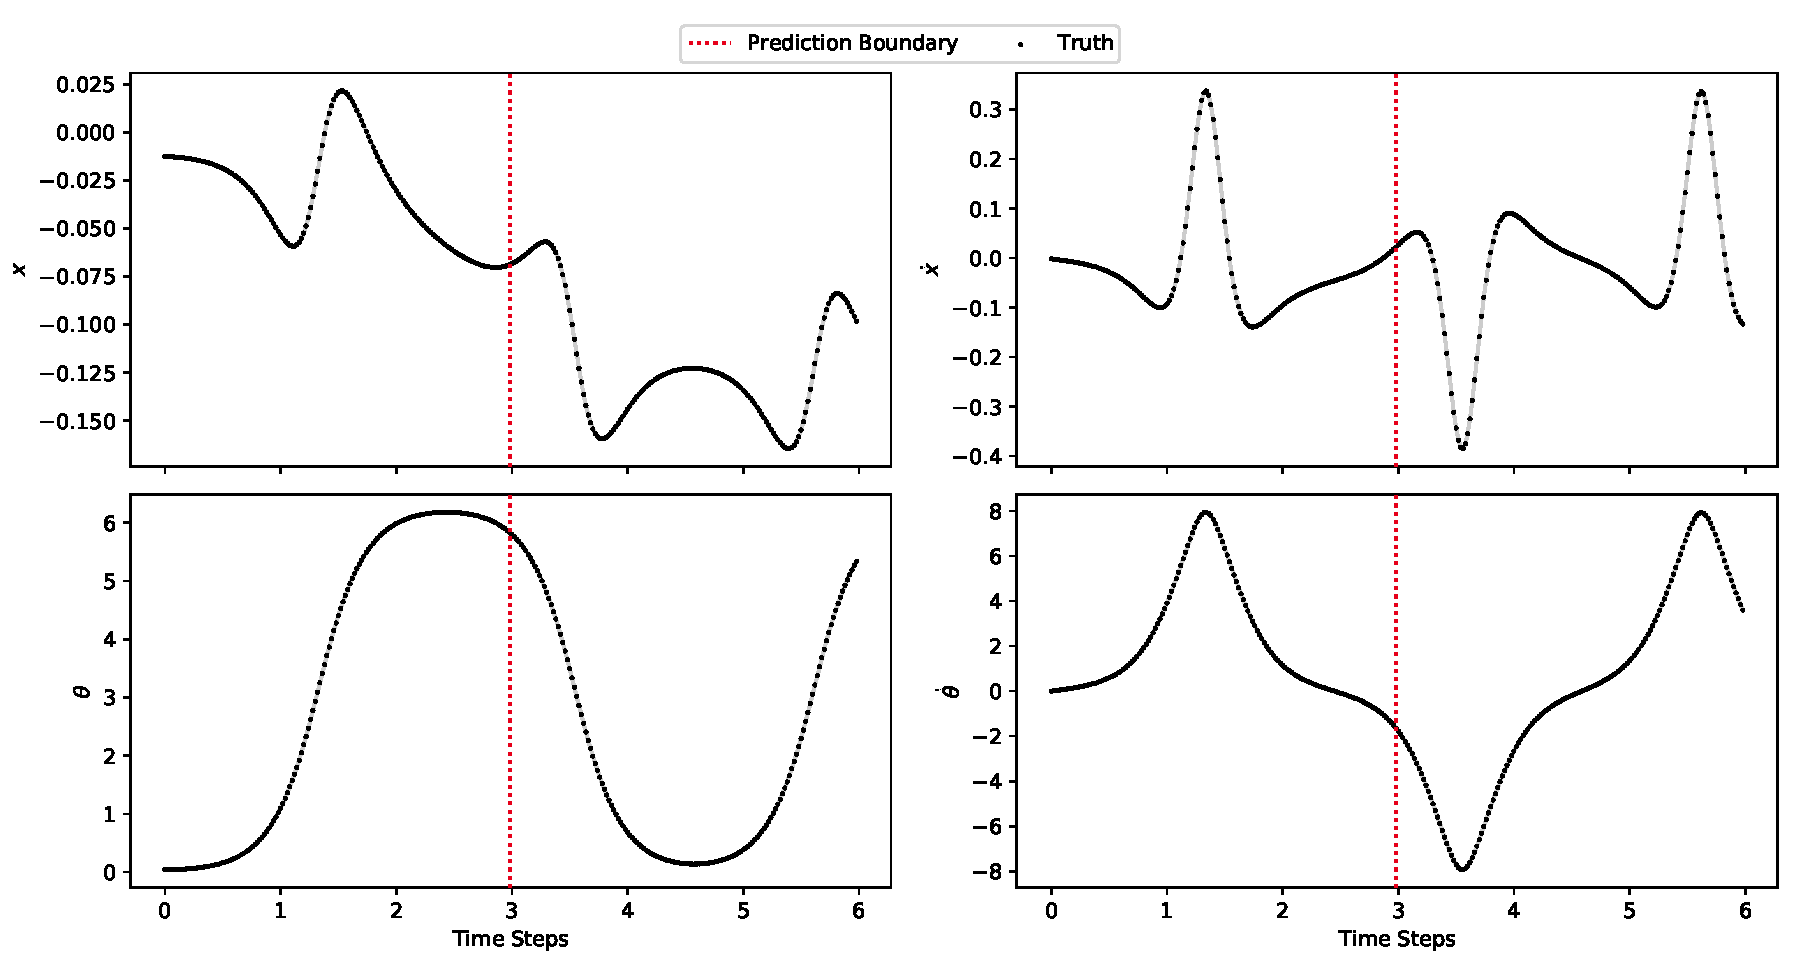
\includegraphics[width=\linewidth]{figures/experiments/environments/observations-cartpole-gym-N0.png}
				\caption[Raw data of the cartpole environment]{Plot of the raw data used for training the Gym cartpole environment. The top plot is the cart position (left) and velocity (right), the row the pole displacement (left) and angular velocity (right). The black dots represent the actual data points, all before the red prediction boundary are used for training, the rest for validation. The faint gray line emphasizes the connection between the data points and that they are actually generated from a dynamical system.}
				\label{fig:envCartpoleGym}
			\end{figure}
		% end

		\subsubsection{Gym Double Pendulum}
			\label{subsubsec:doublePendulum}

			\begin{itemize}
				\item Experiment ID: \texttt{acrobot\_gym}
			\end{itemize}

			The last environment we test on is the double pendulum, implemented in Gym as the \emph{acrobot} (as for the cartpole, we removed all control inputs and modified the initial state to start on top rather than hanging straight down, see~\autoref{lst:topAcrobot}). The double pendulum consists of a pendulum on a fixed joint and a second pendulum attached to the end of the first pendulum. This creates highly nonlinear coupling and is the most common example of a chaotic system~\cite{shinbrotChaosDoublePendulum1992}. We observe the state vector
			\begin{equation*}
				\vec{y} \coloneqq
					\begin{bmatrix}
						\cos\varphi_1 \\
						\sin\varphi_1 \\
						\cos\varphi_2 \\
						\sin\varphi_2 \\
						\dot{\varphi}_1 \\
						\dot{\varphi}_2
					\end{bmatrix}
			\end{equation*}
			where \(\varphi_1\) and \(\varphi_2\) are the displacement of the first and second joint, respectively. See~\autoref{fig:envDoublePendulumGymSketch} for a sketch of the double pendulum. The governing equations of motion are given as:
			\begin{align*}
				\ddot{\varphi}_1 &= \frac{g (\sin\varphi_2 \, \cos\varphi_\Delta - \mu \sin\varphi_1) - (\ell_2 \dot{\varphi}_2^2 + \ell_1 \dot{\varphi}_1^2 \cos\varphi_\Delta) \sin\varphi_\Delta}{\ell_1 (\mu - \cos^2\varphi_\Delta)} \\
				\ddot{\varphi}_2 &= \frac{g \mu (\sin\varphi_2 \, \cos\varphi_\Delta - \mu \sin\varphi_1) + (\mu \ell_1 \dot{\varphi}_1^2 + \ell_2 \dot{\varphi}_2^2 \cos\varphi_\Delta) \sin\varphi_\Delta}{\ell_2 (\mu - \cos^2\varphi_\Delta)}
			\end{align*}
			with \( \varphi_\Delta \coloneqq \varphi_1 - \varphi \), \( \mu \coloneqq 1 + m_1/m_2 \) where \( g = \SI{9.8}{\meter\per\second\squared} \) is the gravitational acceleration, \( m_1 = \SI{1}{\kilogram} \) and \( m_2 = \SI{1}{\kilogram} \) are the masses of the two links and \( \ell_1 = \SI{1}{\meter} \) and \( \ell_2 = \SI{1}{\meter} \) are the lengths of the two links. The Gym environment uses a \ac{rk4} for integrating the \ac{ode} with an evaluation interval of \( h = 0.2 \). We modified the initial position to be drawn from a Gaussian with mean \( \pi \) and standard deviation \( \pi/8 \) and the initial velocity to be drawn from a uniform distribution in the interval \( [-0.1, 0.1] \). We generate \( T = 100 \) time steps of which we use \( T_\train = 75 \) for training and the remaining \(25\) for validation. The raw data is shown in~\autoref{fig:envDoublePendulumGym}.

			\begin{lstlisting}[caption={[Modification of Gym's acrobot environment to start at the top instead of hanging down]Modification of Gym's acrobot environment to start at the top instead of hanging down.}, label=lst:topAcrobot]
import numpy as np
from gym.envs.classic_control import AcrobotEnv

class ModifiedAcrobotEnv(AcrobotEnv):
	def __init__(self):
		super().__init__()

	def reset(self):
		position = self.np_random.normal(np.pi, np.pi / 8.0, size=(2,))
		velocity = self.np_random.uniform(low=-0.1, high=0.1, size=(2,))
		self.state = np.concatenate([position, velocity], axis=0)
		return self._get_ob()
			\end{lstlisting}

			\begin{figure}
				\centering
				\tikzDoublePendulum
				\caption[Illustration of the double pendulum environment]{Illustration of the double pendulum environment. The pendulums have lengths \(\ell_1\) and \(\ell_2\) with the masses \(m_1\) and \(m_2\) attached to the respective ends. The inner pendulum can swing freely around the center while the other pendulum can swing freely around the end of the inner pendulum. Hence, fixing one of the pendulums would transform the system back to a simple pendulum. If both pendulums can swing, the system is chaotic.}
				\label{fig:envDoublePendulumGymSketch}
			\end{figure}

			\begin{figure}
				\centering
				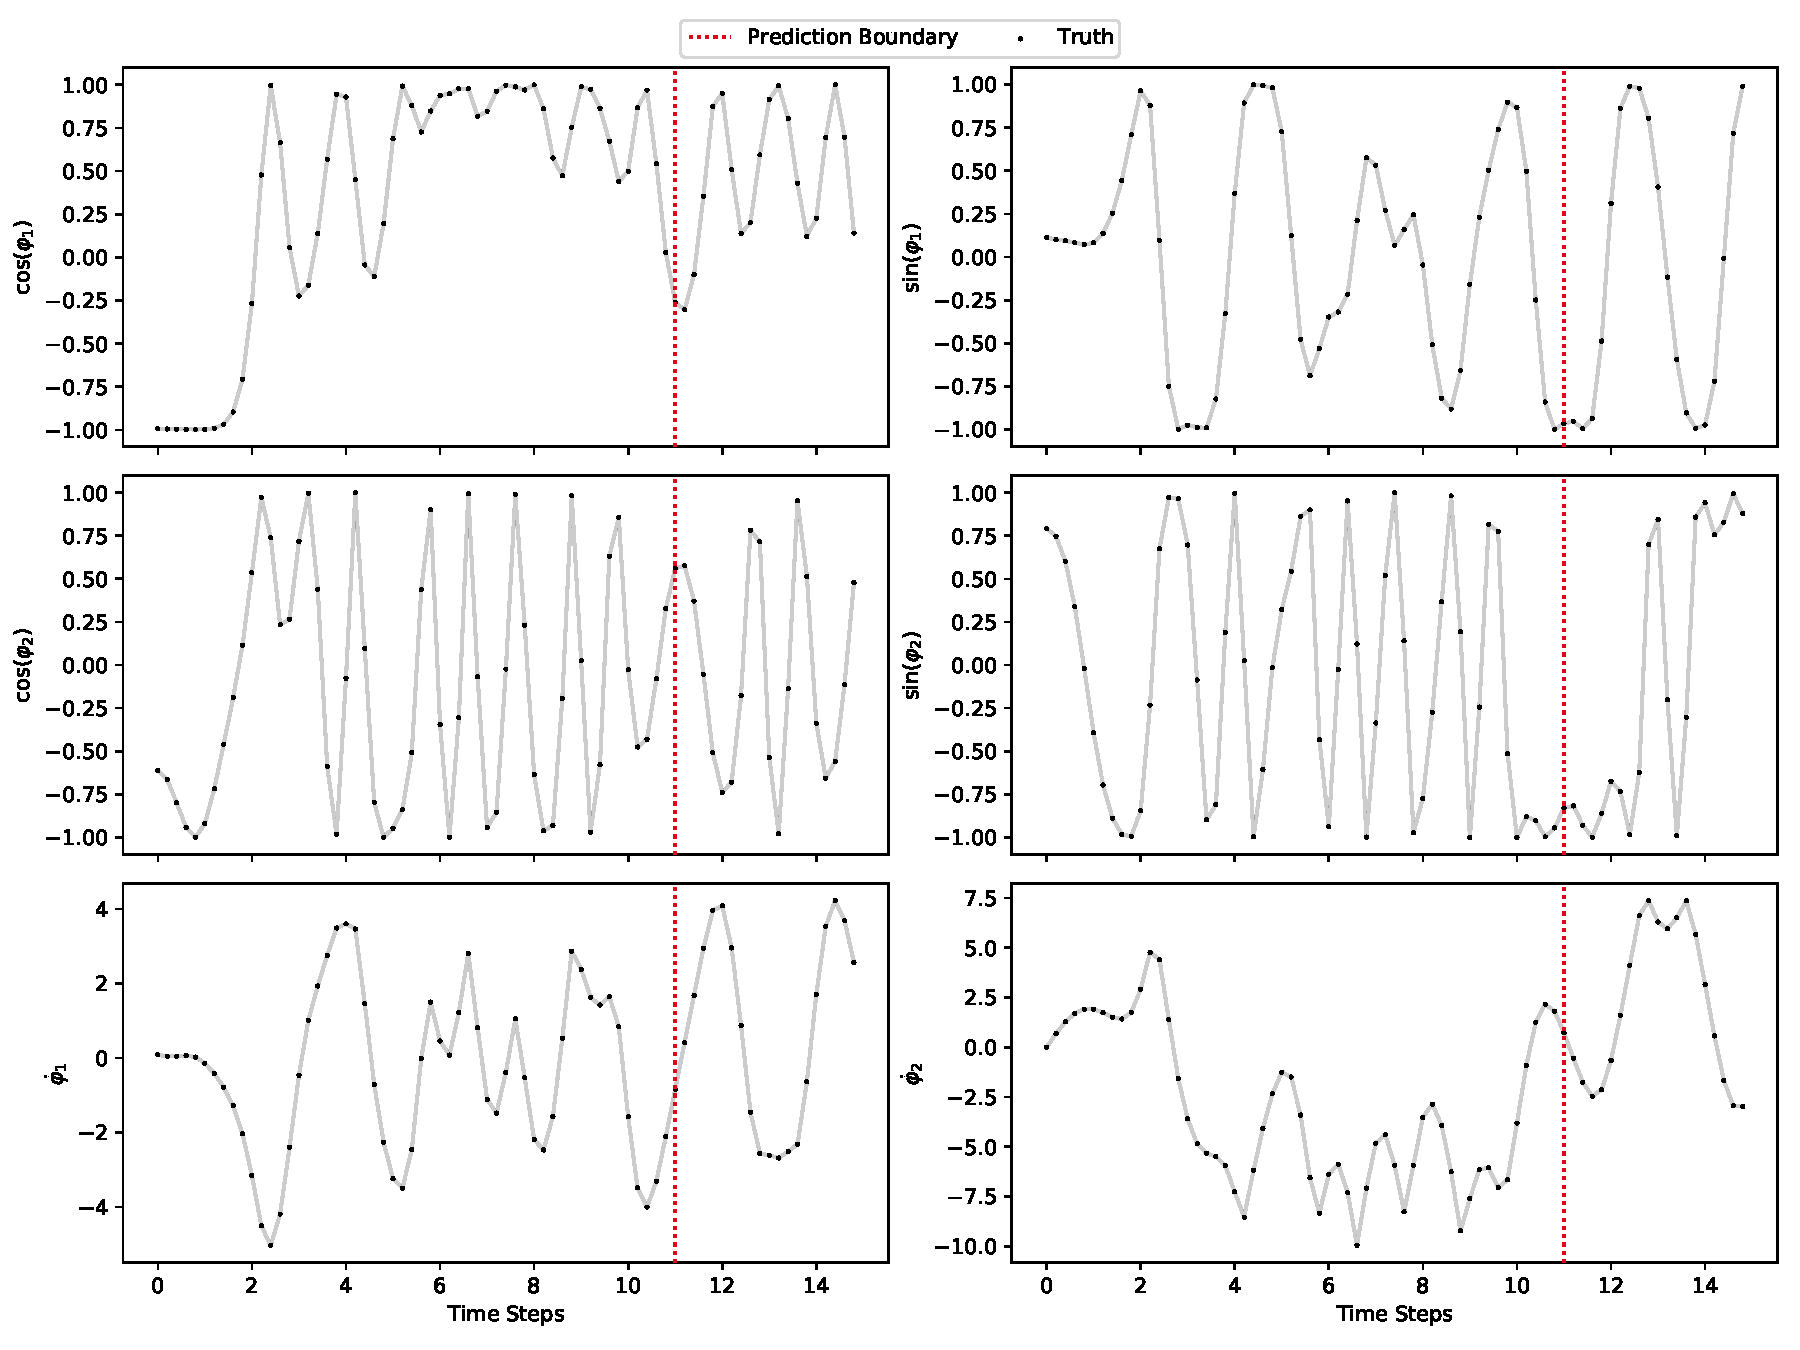
\includegraphics[width=\linewidth]{figures/experiments/environments/observations-acrobot-gym-N0.png}
				\caption[Raw data of the double pendulum environment]{Plot of the raw data used for training the Gym double pendulum environment. The top row shows the cosine/sine of the displacement of the inner pendulum, the middle row shows the cosine/sine of the displacement of the outer pendulum and the bottom row shows the angular velocity of the inner and outer pendulum. The black dots represent the actual data points, all before the red prediction boundary are used for training, the rest for validation. The faint gray line emphasizes the connection between the data points and that they are actually generated from a dynamical system.}
				\label{fig:envDoublePendulumGym}
			\end{figure}
		% end
	% end

	\subsection{Experiment Setup}
		\label{subsec:experimentSetup}

		We now introduce the experiment setup and initialization we used for each environment. For all experiments, we initialized the latent state dynamics matrix \( \mat{A} \) with an identity matrix, the initial state \( \vec{m}_0 \) with a one-vector and all covariance matrices \( \mat{R} \), \( \mat{Q} \) and \( \mat{V}_0 \) with a small diagonal covariance of \( 10^{-5} \). We set the maximum number of \(\vec{g}\)-optimization iterations to \(1000\) for all environments. As described in~\autoref{sec:implementation}, we used a neural network for the observation function with \(\tanh\) activation functions (except for the output layer of course) and a single hidden layer with \(50\) neurons. We used \(100\) maximum iterations for the pendulum, \(200\) for the damped pendulum, \(500\) for the Gym pendulum, \(500\) for the Gym cartpole and \(250\) for the Gym double pendulum.

		For the proof-of-concept environment (the linear system), we used a slightly different setup as the environment is a lot simpler. We used a zero-layer neural network with no activation function, \ie a learnable matrix/linear transformation. We also fixed the latent dimensionality to be \(2\) for the linear system as we only have two states.
	% end

	\subsection{Hyper-Experiments}
		Besides the performance on specific environments, we were interested in how hyperparameters like the latent dimensionality affect the performance of the system. In this section we will discuss and present our experiment setup for the "hyper-experiments". All hyperparameters that are not part of the experiment where set as in in~\autoref{subsec:experimentSetup}.

		If not stated differently, we always ran the experiment with five different seeds\footnote{Namely, we used the seeds \(0\), \(11\), \(42\), \(1234\) and \(1997\).} to average out initialization noise.

		\subsubsection{Influence of the Latent Dimensionality}
			\label{subsec:experimentLatentDim}

			As the latent dimensionality directly influences how well the Koopman matrix can approximate the infinite-dimensional operator, it is one of the most interesting hyperparameters we evaluate. Hence, we evaluate lots of different latent dimensionalities from \( k = 1 \) to \( k = 50 \).
		% end
	% end
% end

\section{Results}
	\label{sec:results}

	In this section we will look at the results of the experiments described above. We organized the section into the different environments and will take a look at both the hyper-experiments first and then the individual results for optimized hyperparameters.

	For evaluating the performance of the model, we use different measures and metrics, both qualitative and quantitative. For a qualitative evaluation, we simply plot the produced data. These plots can get quite noisy as we will see, but they comprise all things we need for a qualitative assessment:
	\begin{itemize}
		\item The \emph{ground truth}, generated as described above with the adequate numerical integration of the equations of motion.
		\item The \emph{smoothed states} as they are produced from the E-step of the \algname algorithm, \ie \(\hat{\vec{s}}_{1:T}\).
		\item The \emph{rollout}, starting both from the learned initial value as well as from the last smoothed state. While the former visualizes the ability of the model to work completely "on its own", the latter shows how well the linear dynamics generalize beyond the training data.
		\item And of course the confidence (\ie the learned variance) around each trajectory.
	\end{itemize}
	For quantitative comparison, we focus on the \ac{nrmse} across all dimensions and time steps, computed as
	\begin{equation*}
		\mathit{NRMSE} = \frac{1}{k} \sum_{i = 1}^{k} \frac{1}{y_\mathrm{max} - y_\mathrm{min}} \sqrt{ \frac{1}{T} \sum_{t = 1}^{T} (y_{t, i} - \tilde{y}_{t, i})^2 }
	\end{equation*}
	where \( y_{t, i} \) is the true data and \( \tilde{y}_{t, i} \) is the corresponding data to evaluate at the \(t\)-th time step of the \(i\)-th dimension. We can compute four different error values: The error over the rollout from start to finish (\( t = 1, 2, \rangedots, T \)), over the training data only (\( t = 1, 2, \rangedots, T_\train \)), over the prediction only (\( t = T_\train, T_\train + 1, \rangedots, T \)) or over the smoothed trajectory (\ie the results from the E-step, \(  \hat{\vec{s}}_{1:T} \)). The latter primarily checks that our algorithm performs correct and that it is even capable of learning the dynamics and it should be near zero or at least below one for a decent parameter choice and model performance. On the other hand, the \ac{nrmse} over the complete rollout describes the generalization abilities. In conjunction with the rollout error over the training and prediction set, we can see where our error comes from. A low error over the training set is the least we should expect while at some environments a high error on the prediction is expected (we will later see when and why).

	Using the \ac{nrmse} instead of the plain \ac{rmse} allows us to compare model performance across the difference dimensions as we are scaling the error to a reasonable interval. For error values below \( 0.01 \), we say that the error is close to zero as it only deviates at most \(1\%\) from the true data. For \(<0.1\) we say it is a good fit, and for \(<0.2\) we say the approximation is decent. However, we have to take these numbers with care as they summarize a lot of data into a single scalar.

	All subsections (of non-proof-of-concept environments) are separated into two main parts: Looking at the hyper-experiment of the latent dimensionality and inspect how well the model performs with different latent dimensionalities. Then we will pick two or three of those latent dimensionalities and look at the qualitative plots of the runs (exemplary evaluation).

	Each exemplary evaluation also contains the ID of the run containing the data we used and the raw data of the runs is added to the \href{https://github.com/fdamken/bachelors-thesis_code}{GitHub repository} along with the code. The documentation for how to generate the plots and so on is also there.

	\subsection{Proof-of-Concept: LGDS}
		For the \ac{lgds} environment, we did not run multiple latent dimensionalities as we already know how many states we have.~\autoref{fig:lgdsRollout} shows the rollout plot for \( k = 3 \) latent dimensions. As expected, both the rollout and the smoothed states perfectly match the true data, even in the prediction time span.

		\begin{figure}
			\centering
			\includegraphics[width=\linewidth]{figures/results/lgds/rollout-observations-N0.png}
			\caption[Rollout of the proof-of-concept LGDS experiment for 3 latent dimensions]{The rollout plot in the observation space of the LGDS environment for \(k = 3\). The left plot shows the first dimension, the right plot the second dimension. The black dots represent the true data of which the model used everything till the red prediction boundary to train on. The blue line is the rollout, starting from the learned initial value (marked with a green star). The orange dash-dotted line is the smoothed data. The dotted orange line then is the rollout starting from the last smoothed state, forming the "smoothed prediction". The orange lines are directly behind the blue ones, hence they are not visible. The shaded regions show the confidence, \ie two times the standard deviation.}
			\label{fig:lgdsRollout}
		\end{figure}
	% end

	\subsection{Pendulum} % TODO: Maybe update with results from GPU…
		\subsubsection{Influence of the Latent Dimensionality}
			For the pendulum experiment, we tested \(50\) latent dimensionalities from \( k = 1 \) to \( k = 50 \).

			We start by having a first look at the \ac{nrmse} of the smoothed trajectory in~\autoref{fig:pendulumRmseSmoothed} to see how many latent dimensions we need at least to get a model that is even slightly capable of learning the pendulum dynamics. We see that the \ac{nrmse} shrinks to near zero (less than \( 0.01 \)). Even for \( k = 1 \), the error is only approximately \( 0.18 \).

			\begin{figure}
				\centering
				\includegraphics[width=0.7\linewidth]{figures/results/pendulum-damped/latent-dim/comparison-rmse-smoothed-normalized-mean-vs-latent-dim.png}
				\caption[Error of the smoothed trajectory on the training data of the pendulum experiment]{The NRMSE of the smoothed trajectory on the training data of the pendulum environment.}
				\label{fig:pendulumRmseSmoothed}
			\end{figure}

			Looking at the \ac{nrmse} of the complete rollout in~\autoref{fig:pendulumRmseComplete}, we see that the error is quite noisy due to initialization. Nevertheless, the error shrinks until \( k \geq 10 \) and then stabilizes around an error of approximately \(0.15\). Comparing the complete rollout error with the training and prediction \ac{nrmse} in~\autoref{fig:pendulumRmseTrain} and~\autoref{fig:pendulumRmsePred}, respectively, we see that the training error falls until \( k \geq 10 \) and then stabilizes around \(0.08\). For the prediction error, we see a similar connection to \( k \geq 10 \), but the error does not shrink as much and always is around \(0.20\).

			\begin{figure}
				\centering
				\begin{subfigure}{0.7\linewidth}
					\centering
					\includegraphics[width=\linewidth]{figures/results/pendulum/latent-dim/comparison-rmse-rollout-normalized-mean-vs-latent-dim.png}
					\caption[Error of the complete rollout on the pendulum environment]{Error of the complete rollout on the pendulum environment.}
					\label{fig:pendulumRmseComplete}
				\end{subfigure} \\
				\begin{subfigure}{0.5\linewidth}
					\centering
					\includegraphics[width=\linewidth]{figures/results/pendulum/latent-dim/comparison-rmse-rollout-train-normalized-mean-vs-latent-dim.png}
					\caption[Error of the training rollout on the pendulum environment]{Error of the rollout on the training data only on the pendulum environment.}
					\label{fig:pendulumRmseTrain}
				\end{subfigure}%
				~
				\begin{subfigure}{0.5\linewidth}
					\centering
					\includegraphics[width=\linewidth]{figures/results/pendulum/latent-dim/comparison-rmse-rollout-prediction-normalized-mean-vs-latent-dim.png}
					\caption[Error of the prediction rollout on the pendulum environment]{Error of the rollout on the prediction only on the pendulum environment.}
					\label{fig:pendulumRmsePred}
				\end{subfigure}
				\caption[Errors on the pendulum environment for different latent dimensions]{Plot of the errors of the pendulum environment for different latent dimensions. The black dots show the measured data, the blue line the average of the data points for a specific latent dimensionality. The blue shaded region shows two times the standard deviation.}
				\label{fig:pendulumRmse}
			\end{figure}
		% end

		\subsubsection{Exemplary Evaluation: 2-Dimensional Latent}
			We now look at an exemplary run for the latent dimensionality \( k = 2 \) (run \texttt{100}). According to the errors, the rollout error should be quite high. On the other hand, the smoothed trajectory should nearly match the true data.~\autoref{fig:pendulumRolloutL02} shows that the rollout and also the rollout of the smoothed trajectory are far off with low confidence, but the true data is in the confidence region. However, the smoothed trajectory follows the true data really good.
		% end

%		\subsubsection{Exemplary Evaluation: 4-Dimensional Latent}
%			We now look at an exemplary run for the latent dimensionality \( k = 4 \) (run \texttt{53}). This run is especially interesting for comparison with~\cite{mortonDeepVariationalKoopman2019a} which we will do in~\autoref{c:discussion}.~\autoref{fig:pendulumRolloutL04} shows the rollout of the model with four latent dimensions. We see that the smoothed trajectory equals the true data as expected, while the rollout captures the dynamics of the system really roughly and the true data lies withing the region of confidence of the rollout.
%
%			\begin{figure}
%				\centering
%				\includegraphics[width=\linewidth]{figures/results/pendulum/run-latent-dim-04/rollout-observations-N0.png}
%				\caption[Rollout of the pendulum experiment for 4 latent dimensions]{The rollout plot in the observation space of the pendulum environment for \(k = 4\). The left plot shows the displacement and the right plot the angular velocity. The black dots represent the true data of which the model used everything till the red prediction boundary to train on. The blue line is the rollout, starting from the learned initial value (marked with a green star). The orange dash-dotted line is the smoothed data. The dotted orange line then is the rollout starting from the last smoothed state, forming the "smoothed prediction". The shaded regions show the confidence, \ie two times the standard deviation.}
%				\label{fig:pendulumRolloutL04}
%			\end{figure}
%		% end

		\subsubsection{Exemplary Evaluation: 10-Dimensional Latent}
			\label{subsubsec:pendulumL10}

			We now look at an exemplary run for the latent dimensionality \( k = 10 \) (run \texttt{10}) as we postulated from the \ac{nrmse} data that this is the boundary of diminishing returns, \ie it does not get much better with higher latent dimensionalities.~\autoref{fig:pendulumRolloutL10} shows the rollout of the model, where the dynamics of the system are captured really good with high confidence. Also the prediction is really good, so that it is hard to distinguish between true data, smoothed prediction and rollout.

			\begin{figure}[H]
				\centering
				\includegraphics[width=\linewidth]{figures/results/pendulum/run-latent-dim-10/rollout-observations-N0.png}
				\caption[Rollout of the pendulum experiment for 10 latent dimensions]{The rollout plot in the observation space of the pendulum environment for \(k = 10\). The left plot shows the displacement and the right plot the angular velocity. The black dots represent the true data of which the model used everything till the red prediction boundary to train on. The blue line is the rollout, starting from the learned initial value (marked with a green star). The orange dash-dotted line is the smoothed data. The dotted orange line then is the rollout starting from the last smoothed state, forming the "smoothed prediction". The shaded regions show the confidence, \ie two times the standard deviation.}
				\label{fig:pendulumRolloutL10}
			\end{figure}
		% end

		\subsubsection{Exemplary Evaluation: 14-Dimensional Latent}
			\label{subsubsec:pendulumL14}

			We now look at an exemplary run for the latent dimensionality \( k = 14 \) (run \texttt{210}) for which we got the smallest overall \ac{nrmse}.~\autoref{fig:pendulumRolloutL14} shows the rollout of the model. In comparison to the 10-dimensional latent, nothing has changed, fulfilling the expectation of diminishing returns with high latent dimensionality.
		% end
	% end

	\subsection{Damped Pendulum} % TODO: Maybe update with results from GPU…
		\subsubsection{Influence of the Latent Dimensionality}
			For the damped pendulum experiment, we tested \(50\) latent dimensionalities from \( k = 1 \) to \( k = 50 \).

			We start by having a first look at the \ac{nrmse} of the smoothed trajectory in~\autoref{fig:pendulumDampedRmseSmoothed} to see how many latent dimensions we need at least to get a model that is even slightly capable of learning the damped pendulum dynamics. We see that the \ac{nrmse} shrinks to near zero (less than \( 0.01 \)) for latent dimensionalities of \( k \geq 2 \). Even for \( k = 1 \), the error is only approximately \( 0.09 \).

			Looking at the \ac{nrmse} of the complete rollout in~\autoref{fig:pendulumDampedRmseComplete}, we see that there is a point of diminishing returns in terms of the latent dimensionality for \( k \geq 10 \), where we get decent errors (around \( 0.05 \)) for all latent dimensionalities. Looking at the parts the complete \ac{nrmse} is composed of, the training and prediction error in~\autoref{fig:pendulumDampedRmseTrain} and~\autoref{fig:pendulumDampedRmsePred}, respectively, we see that the latent dimensionality affects both parts, the training and prediction error. However, the prediction error is generally smaller, which is mostly caused by the value of the state and hence the rollout being smaller.

			\begin{figure}
				\centering
				\includegraphics[width=0.7\linewidth]{figures/results/pendulum-damped/latent-dim/comparison-rmse-smoothed-normalized-mean-vs-latent-dim.png}
				\caption[Error of the smoothed trajectory on the training data of the damped pendulum experiment]{The NRMSE of the smoothed trajectory on the training data of the damped pendulum environment.}
				\label{fig:pendulumDampedRmseSmoothed}
			\end{figure}

			\begin{figure}
				\centering
				\begin{subfigure}{0.7\linewidth}
					\centering
					\includegraphics[width=\linewidth]{figures/results/pendulum-damped/latent-dim/comparison-rmse-rollout-normalized-mean-vs-latent-dim.png}
					\caption[Error of the complete rollout on the damped pendulum environment]{Error of the complete rollout on the damped pendulum environment.}
					\label{fig:pendulumDampedRmseComplete}
				\end{subfigure} \\
				\begin{subfigure}{0.5\linewidth}
					\centering
					\includegraphics[width=\linewidth]{figures/results/pendulum-damped/latent-dim/comparison-rmse-rollout-train-normalized-mean-vs-latent-dim.png}
					\caption[Error of the training rollout on the damped pendulum environment]{Error of the rollout on the training data only on the damped pendulum environment.}
					\label{fig:pendulumDampedRmseTrain}
				\end{subfigure}%
				~
				\begin{subfigure}{0.5\linewidth}
					\centering
					\includegraphics[width=\linewidth]{figures/results/pendulum-damped/latent-dim/comparison-rmse-rollout-prediction-normalized-mean-vs-latent-dim.png}
					\caption[Error of the prediction rollout on the damped pendulum environment]{Error of the rollout on the prediction only on the damped pendulum environment.}
					\label{fig:pendulumDampedRmsePred}
				\end{subfigure}
				\caption[Errors on the damped pendulum environment for different latent dimensions]{Plot of the errors of the damped pendulum environment for different latent dimensions. The black dots show the measured data, the blue line the average of the data points at a specific latent dimensionality. The blue shaded region shows two times the standard deviation.}
				\label{fig:pendulumDampedRmse}
			\end{figure}
		% end

		\subsubsection{Exemplary Evaluation: 2-Dimensional Latent}
			We now look at an exemplary run for the latent dimensionality \( k = 2 \) (run \texttt{2}). According to the errors, the rollout error should be quite high, but the smoothed trajectory should follow the true data really good.~\autoref{fig:pendulumDampedRolloutL02} shows that most trajectories are far off the true trajectory with low confidence, while the smoothed trajectory almost perfectly matches the true data.
		% end

		\subsubsection{Exemplary Evaluation: 10-Dimensional Latent}
			\label{subsubsec:pendulumDampedL10}

			We now look at an exemplary run for the latent dimensionality \( k = 10 \) (run \texttt{110}). We chose this latent dimensionality as it is the boundary of diminishing returns in terms of the \ac{nrmse}, \ie it does not get much better from there on.~\autoref{fig:pendulumDampedRolloutL10} shows the rollout of the model. In comparison to the four-dimensional latent, the behavior of the system is captured pretty good, with a decent confidence. Also the prediction is at nearly the same amplitude as the real data. But the rollout gets phase-shifted in comparison to the true data further in the rollout horizon.

			\begin{figure}
				\centering
				\includegraphics[width=\linewidth]{figures/results/pendulum-damped/run-latent-dim-10/rollout-observations-N0.png}
				\caption[Rollout of the damped pendulum experiment for 10 latent dimensions]{The rollout plot in the observation space of the damped pendulum environment for \(k = 10\). The left plot shows the displacement and the right plot the angular velocity. The black dots represent the true data of which the model used everything till the red prediction boundary to train on. The blue line is the rollout, starting from the learned initial value (marked with a green star). The orange dash-dotted line is the smoothed data. The dotted orange line then is the rollout starting from the last smoothed state, forming the "smoothed prediction". The shaded regions show the confidence, \ie two times the standard deviation.}
				\label{fig:pendulumDampedRolloutL10}
			\end{figure}
		% end

		\subsubsection{Exemplary Evaluation: 24-Dimensional Latent}
			We now look at an exemplary run for the latent dimensionality \( k = 30 \) (run \texttt{130}) for which we got the smallest overall \ac{nrmse}.~\autoref{fig:pendulumDampedRolloutL30} shows the rollout of the model. In comparison to the ten-dimensional latent, the model is a less confident but the rollout is nearly the same as the rollout of the ten-dimensional latent.
		% end
	% end

	\subsection{Gym Pendulum} % Finished!
		\subsubsection{Influence of the Latent Dimensionality}
			\label{subsubsec:gymPendulumLatents}

			For the Gym pendulum experiment, we tested \(50\) latent dimensionalities from \( k = 1 \) to \( k = 50 \). The difference of the Gym pendulum in comparison to the pendulum from before is that we do not measure the angle directly but use the sine/cosine of the angle, directly encoding the symmetry of a swing-around into the features. This environment is extremely numerically brittle, thus we have less data points for higher latent dimensionalities (to the right of the plots).

			We start by having a first look at the \ac{nrmse} of the smoothed trajectory in~\autoref{fig:gymPendulumRmseSmoothed} to see how many latent dimensions we need at least to get a model that is even slightly capable of learning dynamics. We see that the \ac{nrmse} shrinks to near zero (less than \( 0.01 \)) for latent dimensionalities of \( k \geq 2 \). Even for \( k = 1 \), the error is only approximately \( 0.09 \).

			Looking at the \ac{nrmse} of the complete rollout in~\autoref{fig:gymPendulumRmseComplete}, we see a slight improvement at the beginning, which is, looking at the training and prediction error in~\autoref{fig:gymPendulumRmseTrain} and~\autoref{fig:gymPendulumRmsePred}, respectively, fully caused by the training error. Looking at the prediction error, we see that the error does not change much with different latent dimensionalities\footnote{The spike on the right is possibly due to bad initialization and is only chosen as the mean as all other seeds crashed due to negative definite matrices.}. In comparison, the training error shrinks to near zero (less than \( 0.01 \)) for latent dimensionalities \( k \geq 7 \). Hence, we expect the model not to predict well behind the prediction boundary.

			\begin{figure}
				\centering
				\includegraphics[width=0.7\linewidth]{figures/results/pendulum-gym/latent-dim/comparison-rmse-smoothed-normalized-mean-vs-latent-dim.png}
				\caption[Error of the smoothed trajectory on the training data of the Gym pendulum experiment]{The NRMSE of the smoothed trajectory on the training data of the Gym pendulum environment.}
				\label{fig:gymPendulumRmseSmoothed}
			\end{figure}

			\begin{figure}
				\centering
				\begin{subfigure}{0.7\linewidth}
					\centering
					\includegraphics[width=\linewidth]{figures/results/pendulum-gym/latent-dim/comparison-rmse-rollout-normalized-mean-vs-latent-dim.png}
					\caption[Error of the complete rollout on the Gym pendulum environment]{Error of the complete rollout on the Gym pendulum environment.}
					\label{fig:gymPendulumRmseComplete}
				\end{subfigure} \\
				\begin{subfigure}{0.5\linewidth}
					\centering
					\includegraphics[width=\linewidth]{figures/results/pendulum-gym/latent-dim/comparison-rmse-rollout-train-normalized-mean-vs-latent-dim.png}
					\caption[Error of the training rollout on the Gym pendulum environment]{Error of the rollout on the training data only on the Gym pendulum environment.}
					\label{fig:gymPendulumRmseTrain}
				\end{subfigure}%
				~
				\begin{subfigure}{0.5\linewidth}
					\centering
					\includegraphics[width=\linewidth]{figures/results/pendulum-gym/latent-dim/comparison-rmse-rollout-prediction-normalized-mean-vs-latent-dim.png}
					\caption[Error of the prediction rollout on the Gym pendulum environment]{Error of the rollout on the prediction only on the Gym pendulum environment.}
					\label{fig:gymPendulumRmsePred}
				\end{subfigure}
				\caption[Errors on the Gym pendulum environment for different latent dimensions]{Plot of the errors of the Gym pendulum environment for different latent dimensions. The black dots show the measured data, the blue line the average of the data points at a specific latent dimensionality. The blue shaded region shows two times the standard deviation.}
				\label{fig:gymPendulumRmse}
			\end{figure}
		% end

		\subsubsection{Exemplary Evaluation: 2-Dimensional Latent}
			We now look at an exemplary run for the latent dimensionality \( k = 2 \) (run \texttt{2}). According to the errors, the rollout trajectory should be off the true data, but the smoothed trajectory should be mostly on the true data.~\autoref{fig:gymPendulumRolloutL02} shows exactly this behavior: all trajectories are far off the true trajectory with the exception of the smoothed trajectory that almost matches the true data.
		% end

		\subsubsection{Exemplary Evaluation: 4-Dimensional Latent}
			\label{subsubsec:gymPendulumL04}

			We now look at an exemplary run for the latent dimensionality \( k = 4 \) (run \texttt{104}). This run is especially interesting for comparison with~\cite{mortonDeepVariationalKoopman2019a} which we will do in~\autoref{c:discussion}.~\autoref{fig:gymPendulumRolloutL04} shows the rollout of the model with four latent dimensions. We see that the smoothed trajectory equals the true data as expected and so does the training rollout. However, on the prediction the rollout only roughly follows the true data, capturing the dynamics of the system only roughly.

			\begin{figure}
				\centering
				\includegraphics[width=\linewidth]{figures/results/pendulum-gym/run-latent-dim-04/rollout-observations-N0.png}
				\caption[Rollout of the Gym pendulum experiment for 4 latent dimensions]{The rollout plot in the observation space of the Gym pendulum environment for \(k = 4\). The left plot shows the displacement and the right plot the angular velocity. The black dots represent the true data of which the model used everything till the red prediction boundary to train on. The blue line is the rollout, starting from the learned initial value (marked with a green star). The orange dash-dotted line is the smoothed data. The dotted orange line then is the rollout starting from the last smoothed state, forming the "smoothed prediction". The shaded regions show the confidence, \ie two times the standard deviation.}
				\label{fig:gymPendulumRolloutL04}
			\end{figure}
		% end

		\subsubsection{Exemplary Evaluation: 7-Dimensional Latent}
			\label{subsubsec:gymPendulumL07}

			We now look at an exemplary run for the latent dimensionality \( k = 7 \) (run \texttt{157}) as we postulated from the \ac{nrmse} data that this is the boundary of diminishing returns, \ie it does not get much better with higher latent dimensionalities.~\autoref{fig:gymPendulumRolloutL7} shows the rollout of the model. We see that the training rollout and the smoothed trajectory is good, as expected, but the prediction does not capture the dynamics of the system.
		% end
	% end

	\subsection{Gym Cartpole} % Finished!
		\subsubsection{Influence of the Latent Dimensionality}
			\label{subsubsec:cartpoleLatents}

			For the cartpole experiment, we tested \(50\) latent dimensionalities from \( k = 1 \) to \( k = 50 \).

			We start by having a first look at the \ac{nrmse} of the smoothed trajectory in~\autoref{fig:cartpoleRmseSmoothed} to see how many latent dimensions we need at least to get a model that is even slightly capable of learning the cartpole dynamics. We see that the \ac{nrmse} shrinks to near zero (approximately \(0.001\)) for latent dimensionalities of \( k \geq 2 \). Hence, we need at least \(2\) latent dimensions to learn the dynamics.

			Looking at the \ac{nrmse} of the complete rollout in~\autoref{fig:cartpoleRmseComplete}, we see that the error does not shrink much any more for latent dimensionalities of \( k \geq 10 \), where the error stabilizes around \(0.23\). Looking at the training and prediction plots in~\autoref{fig:cartpoleRmseTrain} and~\autoref{fig:cartpoleRmsePred}, respectively, we see that the training error falls a lot until \( k \geq 10 \) latent dimensions where the error stabilized near zero, while the prediction error does not fall much after the first few latent dimensionalities. Hence, we can predict that our model learns the training rollout well, but does not generalize behind the prediction boundary.

			\begin{figure}
				\centering
				\includegraphics[width=0.7\linewidth]{figures/results/cartpole-gym/latent-dim/comparison-rmse-smoothed-normalized-mean-vs-latent-dim.png}
				\caption[Error of the smoothed trajectory on the training data of the cartpole experiment]{The NRMSE of the smoothed trajectory on the training data of the cartpole environment.}
				\label{fig:cartpoleRmseSmoothed}
			\end{figure}

			\begin{figure}
				\centering
				\begin{subfigure}{0.7\linewidth}
					\centering
					\includegraphics[width=\linewidth]{figures/results/cartpole-gym/latent-dim/comparison-rmse-rollout-normalized-mean-vs-latent-dim.png}
					\caption[Error of the complete rollout on the cartpole environment]{Error of the complete rollout from on the cartpole environment.}
					\label{fig:cartpoleRmseComplete}
				\end{subfigure} \\
				\begin{subfigure}{0.5\linewidth}
					\centering
					\includegraphics[width=\linewidth]{figures/results/cartpole-gym/latent-dim/comparison-rmse-rollout-train-normalized-mean-vs-latent-dim.png}
					\caption[Error of the training rollout on the cartpole environment]{Error of the rollout on the training data only on the cartpole environment.}
					\label{fig:cartpoleRmseTrain}
				\end{subfigure}%
				~
				\begin{subfigure}{0.5\linewidth}
					\centering
					\includegraphics[width=\linewidth]{figures/results/cartpole-gym/latent-dim/comparison-rmse-rollout-prediction-normalized-mean-vs-latent-dim.png}
					\caption[Error of the prediction rollout on the cartpole environment]{Error of the rollout on the prediction only on the cartpole environment.}
					\label{fig:cartpoleRmsePred}
				\end{subfigure}
				\caption[Errors on the cartpole environment for different latent dimensions]{Plot of the errors of the cartpole environment for different latent dimensions. The black dots show the measured data, the blue line the average of the data points at a specific latent dimensionality. The blue shaded region shows two times the standard deviation. The data points on the right side of the plot get increasingly sparse as the algorithm gets increasingly numerically brittle for higher latent dimensionalities.}
				\label{fig:cartpoleRmse}
			\end{figure}
		% end

		\subsubsection{Exemplary Evaluation: 2-Dimensional Latent}
			We now look at an exemplary run for the latent dimensionality \( k = 2 \) (run \texttt{2}). As we have already seen, the rollout should not perform too god, but the smoothed trajectory should be really accurate. Looking at~\autoref{fig:cartpoleRolloutL02}, we see that nearly all trajectories are off the true trajectory. Only the smoothed trajectory fits the data perfectly (until the prediction boundary). We can also see that the rollout starts to go near the true data, learning roughly how the true data looks.
		% end

		\subsubsection{Exemplary Evaluation: 10-Dimensional Latent}
			\label{subsubsec:cartpoleL10}

			We now look at an exemplary run for the latent dimensionality \( k = 10 \) (run \texttt{10}). According to the \ac{nrmse} of the training data, this should perform decent on the training data and, according to the \ac{nrmse} on the prediction, bad on the prediction.~\autoref{fig:cartpoleRolloutL10} shows that the rollout and the smoothed trajectory actually follow the true data, while the rollout does not match the true data after the prediction boundary, but roughly forecasts the qualitative behavior. Interestingly, the confidence in the rollout of the pendulum displacement and velocity is a lot higher than the confidence in the rollout of the cart position and velocity.

			\begin{figure}
				\centering
				\includegraphics[width=\linewidth]{figures/results/cartpole-gym/run-latent-dim-10/rollout-observations-N0.png}
				\caption[Rollout of the cartpole experiment for 10 latent dimensions]{The rollout plot in the observation space of the cartpole environment for \(k = 10\). The top plot is the cart position (left) and velocity (right), the row the pole displacement (left) and angular velocity (right). The black dots represent the true data of which the model used everything until the red prediction boundary to train on. The blue line is the rollout, starting from the learned initial value (marked with a green star). The orange dash-dotted line is the smoothed data. The dotted orange line then is the rollout starting from the last smoothed state, forming the "smoothed prediction". The shaded regions show the confidence, \ie two times the standard deviation. As the variances in the top plots are very high, see~\autoref{fig:cartpoleRolloutL10Appendix} in~\autoref{app:remainingPlots} for the plot without the confidence.}
				\label{fig:cartpoleRolloutL10}
			\end{figure}
		% end

		\subsubsection{Exemplary Evaluation: 16-Dimensional Latent}
			\label{subsubsec:cartpoleL16}

			We now look at an exemplary run for the latent dimensionality \( k = 16 \) (run \texttt{166}), the run which had the lowest \ac{nrmse} over the complete rollout data. Still, according to the \ac{nrmse} of the prediction, we do not expect a good prediction.~\autoref{fig:cartpoleRolloutL16} confirms this, as the rollout on the training data follows the true data closely while the prediction is off the true trajectory. Compared to the 14-dimensional latent, we do not see much improvement in the prediction.
		% end
	% end

	\subsection{Gym Double Pendulum} % Finished! Run again with more latent dims if there is time…
		\todo{Gym Acrobot: If there is time, run again with k = 51 to k = 100.}

		\subsubsection{Influence of the Latent Dimensionality}
			For the double pendulum experiment, we tested \(50\) latent dimensionalities from \( k = 1 \) to \( k = 50 \).

			We start by having a first look at the \ac{nrmse} of the smoothed trajectory in~\autoref{fig:acrobotRmseSmoothed} to see how many latent dimensions we need at least to get a model that is even slightly capable of learning the double pendulum dynamics. We see that the \ac{nrmse} shrinks below \(0.05\) for latent dimensionalities of \( k \geq 3 \), so we need at least \(3\) latent dimensions to get a decent model.

			Looking at the \ac{nrmse} of the complete rollout in~\autoref{fig:acrobotRmseComplete}, we see that the error shrinks until \( k \geq 6 \) latent dimensions and than stabilizes to an error around \( 0.27 \). Looking at the training and prediction error in~\autoref{fig:acrobotRmseTrain} and~\autoref{fig:acrobotRmsePred}, we see that mostly only the training error shrinks while the prediction errors seems to be random noise. For the training error, however, we see that the error shrinks until \( k \geq 18 \) and then stabilized around \( 0.17 \). Hence, we can assume that our model does not generalize well (we will assess this in~\autoref{c:discussion}). On the other hand, our rollout on the training data should be a good fit.

			\begin{figure}
				\centering
				\includegraphics[width=0.7\linewidth]{figures/results/acrobot-gym/latent-dim/comparison-rmse-smoothed-normalized-mean-vs-latent-dim.png}
				\caption[Error of the smoothed trajectory on the training data of the double pendulum experiment]{The NRMSE of the smoothed trajectory on the training data of the double pendulum environment.}
				\label{fig:acrobotRmseSmoothed}
			\end{figure}

			\begin{figure}
				\centering
				\begin{subfigure}{0.7\linewidth}
					\centering
					\includegraphics[width=\linewidth]{figures/results/acrobot-gym/latent-dim/comparison-rmse-rollout-normalized-mean-vs-latent-dim.png}
					\caption[Error of the complete rollout on the double pendulum environment]{Error of the complete rollout from on the double pendulum environment.}
					\label{fig:acrobotRmseComplete}
				\end{subfigure} \\
				\begin{subfigure}{0.5\linewidth}
					\centering
					\includegraphics[width=\linewidth]{figures/results/acrobot-gym/latent-dim/comparison-rmse-rollout-train-normalized-mean-vs-latent-dim.png}
					\caption[Error of the training rollout on the double pendulum environment]{Error of the rollout on the training data only on the double pendulum environment.}
					\label{fig:acrobotRmseTrain}
				\end{subfigure}%
				~
				\begin{subfigure}{0.5\linewidth}
					\centering
					\includegraphics[width=\linewidth]{figures/results/acrobot-gym/latent-dim/comparison-rmse-rollout-prediction-normalized-mean-vs-latent-dim.png}
					\caption[Error of the prediction rollout on the double pendulum environment]{Error of the rollout on the prediction only on the double pendulum environment.}
					\label{fig:acrobotRmsePred}
				\end{subfigure}
				\caption[Errors on the double pendulum environment for different latent dimensions]{Plot of the errors of the double pendulum environment for different latent dimensions. The black dots show the measured data, the blue line the average of the data points at a specific latent dimensionality. The blue shaded region shows two times the standard deviation. The data points on the right side of the plot get increasingly sparse as the algorithm gets increasingly numerically brittle for higher latent dimensionalities.}
				\label{fig:acrobotRmse}
			\end{figure}
		% end

		\subsubsection{Exemplary Evaluation: 3-Dimensional Latent}
			We now look at an exemplary run for the latent dimensionality \( k = 3 \) (run \texttt{153}). As we have already seen, the rollout should not perform well, but the smoothed trajectory should be really accurate. Looking at~\autoref{fig:acrobotRolloutL03}, we see that nearly all trajectories are far off the true trajectory. Only the smoothed trajectory follows the data decently (until the prediction boundary, of course).
		% end

		\subsubsection{Exemplary Evaluation: 18-Dimensional Latent}
			We now look at an exemplary run for the latent dimensionality \( k = 18 \) (run \texttt{168}). We chose this latent dimensionality as it is at the boundary before the training error does not get much batter in terms of the \ac{nrmse}.~\autoref{fig:acrobotRolloutL18} shows the rollout of the model. We see that the rollout on the training trajectory nearly perfectly follows the true data, while the prediction is quite off the true trajectory, not even capturing some of the motion. This is especially bad as the model is quite confident about the state.

			\begin{figure}
				\centering
				\includegraphics[width=0.9\linewidth]{figures/results/acrobot-gym/run-latent-dim-18/rollout-observations-N0.png}
				\caption[Rollout of the double pendulum experiment for 18 latent dimensions]{The rollout plot in the observation space of the double pendulum environment for \(k = 18\). The top row shows the cosine/sine of the displacement of the inner pendulum, the middle row shows the cosine/sine of the displacement of the outer pendulum and the bottom row shows the angular velocity of the inner and outer pendulum. The black dots represent the true data of which the model used everything till the red prediction boundary to train on. The blue line is the rollout, starting from the learned initial value (marked with a green star). The orange dash-dotted line is the smoothed data. The dotted orange line then is the rollout starting from the last smoothed state, forming the "smoothed prediction". The shaded regions show the confidence, \ie two times the standard deviation.}
				\label{fig:acrobotRolloutL18}
			\end{figure}
		% end

		\subsubsection{Exemplary Evaluation: 30-Dimensional Latent}
			We now look at an exemplary run for the latent dimensionality \( k = 30 \) (run \texttt{80}) for which we got the smallest overall \ac{nrmse}.~\autoref{fig:acrobotRolloutL30} shows the rollout of the model. In comparison to the 18-dimensional latent, the rollout is not nearly as good. However, the low confidence in the prediction produces is better than for the 18-dimensional latent as more parts of the true trajectory lie within the region of confidence.
		% end
	% end
% end

	\chapter{Discussion}
\label{c:discussion}
\IMRADlabel{discussion}



In this chapter we will analyze the results from~\autoref{c:experiments} and set them into context with results from related work. We will discuss the performance on the different environments first and then compare our results with the results of some related work.

\section{Model Performance}
	\subsection{Proof-of-Concept: LGDS}
		As we have seen in~\autoref{fig:lgdsRollout}, the \ac{lgds} proof-of-concept environment works pretty well and the prediction perfectly matches the true data. The model has an \ac{nrmse} of approximately \( 0.0001 \) for every metric. This shows that we are still able to learn linear dynamical systems. We expected this result as we have proven that our algorithm is equivalent to the \ac{lgds} inference algorithm for linear systems in~\autoref{app:ngkExactness}. Hence, our algorithm does not reduce the "power" of the linear algorithm on linear systems and only extends its usability to nonlinear systems.
	% end

	\subsection{Pendulum}
		\label{subsec:discussPendulum}

		The pendulum is the first nonlinear environment we assess.

		As we have seen in the experiment for different latent dimensionalities, we need at least ten latent dimensions to model the pendulum with a decent prediction error, where we expected some downsides on the prediction and expected a really good rollout in the training area. As we have seen in the results for a ten-dimensional latent in~\autoref{subsubsec:pendulumL10}, we see a good rollout in the training area and also a good prediction for the pendulum position, but a slightly smaller amplitude in the velocity plot. This corresponds to an energy loss of the pendulum that should not happen as it is undamped.~\autoref{fig:pendulumEnergyL10} highlights this by showing the total, kinetic and potential energy of the system, where the rollout energy changes with time which should not happen. However, the potential energy almost matches the true potential energy, supporting our inspection that the angular displacement is well fit. The kinetic energy generated by the velocity is, on the other hand, a bit off. We can further inspect this behavior by looking at the rollout in the latent space in~\autoref{fig:pendulumLatentRolloutL10}. We see that the energy loss is primarily happening in the tenth dimension. Looking at the real parts of the eigenvalues of the latent state dynamics matrix,
		\begin{equation*}
			\sigma = \{ 1.00, 1.00, 1.00, 0.96, 0.65, 0.67, 0.86, 0.80, 0.73, 0.75 \}
		\end{equation*}
		we see that not all are close to one, \ie they vanish after some time. This directly corresponds to the energy loss in the system (the eigenvalues of a system capture the time evolution). We also see that the tenth dimension has a really high variance in its states, indicating that the model already has enough latent dimensions to explain the dynamics. Looking at the rollout of a nine-dimensional latent (run \texttt{58}) in~\autoref{fig:pendulumRolloutL09}, however, we see that the energy loss is still there. It does not make sense to inspect higher-dimensional latent spaces as we have seen in the latent dimensionalities experiment that the error does not shrink much. Additionally, the 14-dimensional latent that we inspected in~\autoref{subsubsec:pendulumL10} also looses energy. We do not expect this to get better with higher latent dimensionalities. Also, higher dimensionalities impose numerical instability, a phenomenon we will address in~\autoref{subsec:discussPerformanceNumerics}.

		For this environment, we get really small confidences with the true trajectory still being in the region of confidence. We also see that the variance is higher on the turns of the pendulum which makes sense as that is the most critical part of the movement.

		While these first results cast a shadow on our model performance, the energy loss builds hope for the damped pendulum to work out well.

		\begin{figure}
			\centering
			\begin{subfigure}{0.7\linewidth}
				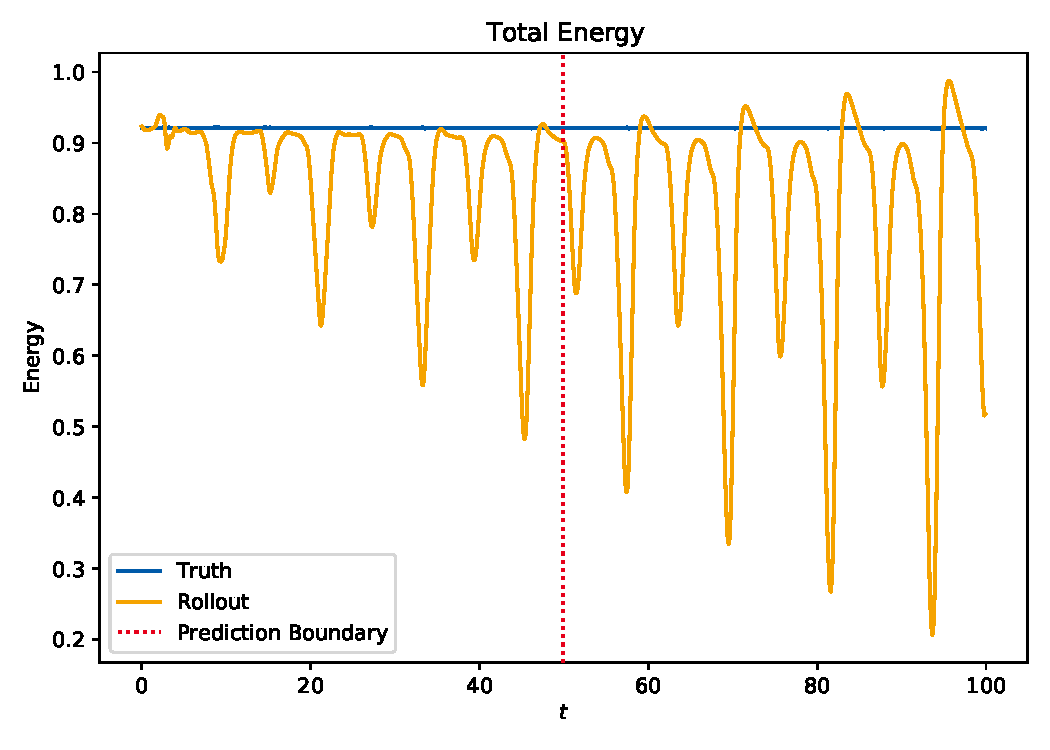
\includegraphics[width=\linewidth]{figures/results/pendulum/run-latent-dim-10/energy-R10-N0-total.png}
			\end{subfigure} \\
			\begin{subfigure}{0.5\linewidth}
				\centering
				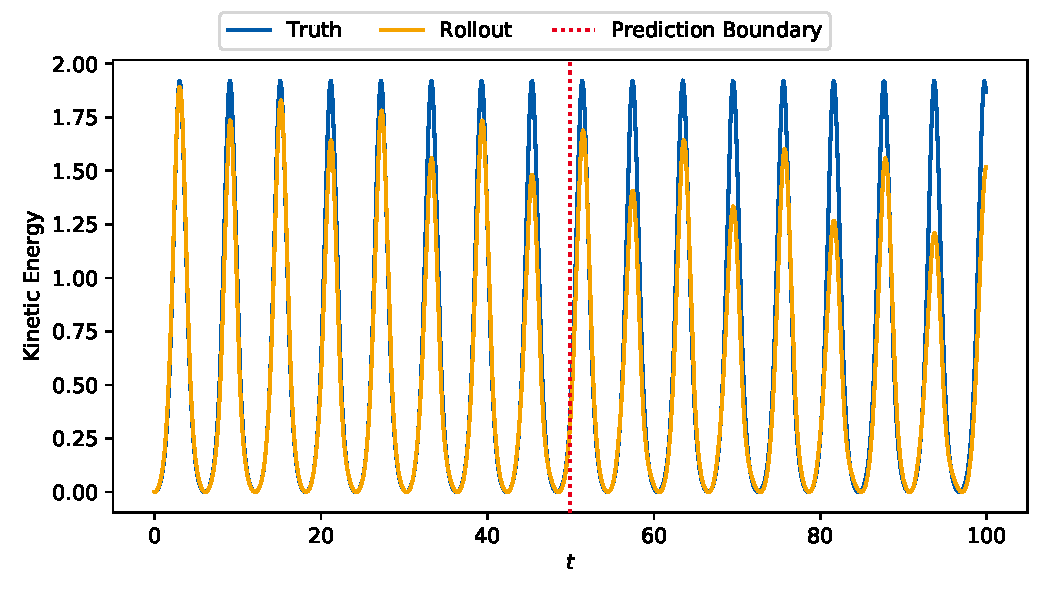
\includegraphics[width=\linewidth]{figures/results/pendulum/run-latent-dim-10/energy-R10-N0-kinetic.png}
			\end{subfigure}%
			~
			\begin{subfigure}{0.5\linewidth}
				\centering
				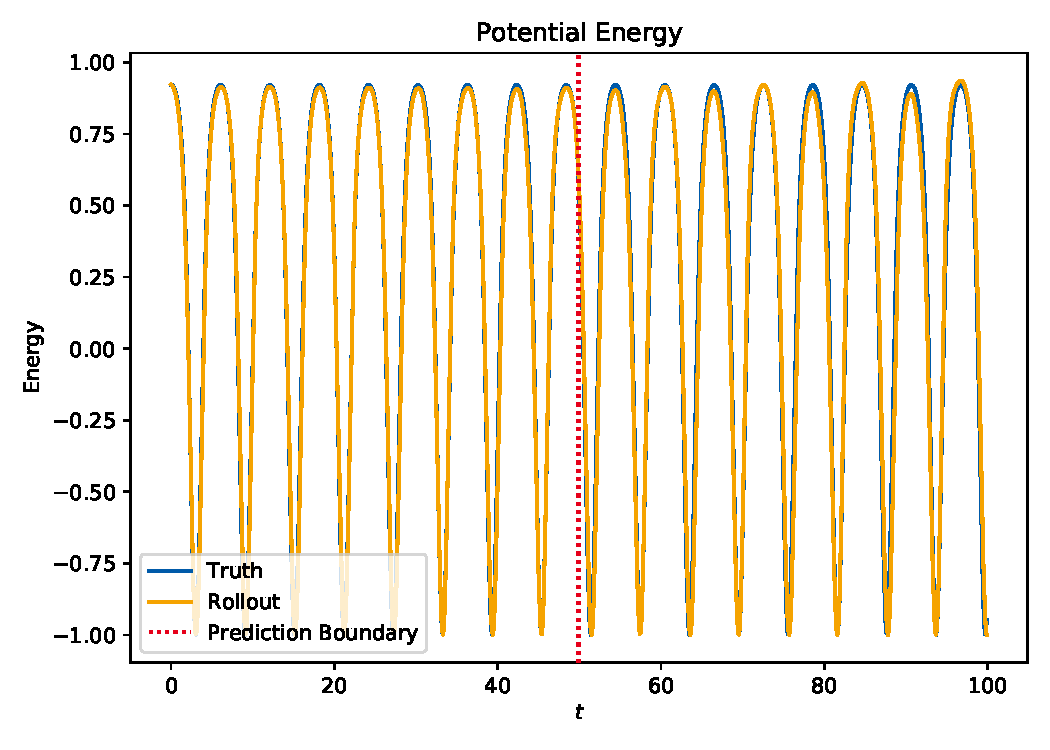
\includegraphics[width=\linewidth]{figures/results/pendulum/run-latent-dim-10/energy-R10-N0-potential.png}
			\end{subfigure}
			\caption[Total energy of the undamped pendulum]{Total energy of the undamped pendulum composed of the kinetic energy on the bottom left and the potential energy on the bottom right. The blue line represents the true energy, calculated from the training and validation data. The orange line is the energy calculated from the rollout. As usual, the red line is the prediction boundary up until all training data was used; afterwards, the model predicted the rest of the data.}
			\label{fig:pendulumEnergyL10}
		\end{figure}

		\begin{figure}
			\centering
			\includegraphics[width=\linewidth]{figures/results/pendulum/run-latent-dim-10/rollout-latents-N0.png}
			\caption[Latent rollout of the pendulum experiment for 10 latent dimensions]{Rollout of the latent dimensions of the pendulum environment for \(k = 10 \) latents.}
			\label{fig:pendulumLatentRolloutL10}
		\end{figure}

		\begin{figure}
			\centering
			\includegraphics[width=\linewidth]{figures/results/pendulum/run-latent-dim-09/rollout-observations-N0.png}
			\caption[Rollout of the pendulum experiment for 9 latent dimensions]{The rollout plot in the observation space of the pendulum environment for \(k = 9\). The left plot shows the displacement and the right plot the angular velocity. The black dots represent the true data of which the model used everything till the red prediction boundary to train on. The blue line is the rollout, starting from the learned initial value (marked with a green star). The orange dash-dotted line is the smoothed data. The dotted orange line then is the rollout starting from the last smoothed state, forming the "smoothed prediction". The shaded regions show the confidence, \ie two times the standard deviation.}
			\label{fig:pendulumRolloutL09}
		\end{figure}
	% end

	\subsection{Damped Pendulum}
		\label{subsec:discussDampedPendulum}

		As for the undamped pendulum, we have seen in the experiment with different latent dimensionalities that we need at least ten latent dimensions. For ten dimensions, we get a decent \ac{nrmse} on both training and prediction. We have seen this behavior in~\autoref{subsubsec:pendulumDampedL10} and in the rollout plot in~\autoref{fig:pendulumDampedRolloutL10}. In contrast to the undamped pendulum, the amplitudes of the oscillations are now on the correct heights, so we definitely learn the energy loss of the system. We can also see this behavior in the plot of the total, kinetic and potential energy in~\autoref{fig:pendulumDampedEnergyL10}. We see in the total and the kinetic and potential energy that the damped pendulum model is really close to the real energy levels, in all energy types. This supports the first interpretation of the rollout that we really learn the energy loss. On the other hand, the rollout is phase-shifted to the real trajectory, sometimes even predicting the pendulum to be on the opposite side of a swing. Looking at the rollout in the latent space in~\autoref{fig:pendulumDampedLatentRolloutL10}, we see a similar behavior in the latent space, so our learned observation function seems to be correct, but the latent dynamics are a bit off.

		Improving this might be possible by fixing the observation function and optimizing just the state dynamics matrix on its own. This reduces the parameters the algorithm has to learn by a lot, possibly yielding a more accurate rollout. But overall we are satisfied with this result as we learn the energy loss and get a confidence that is not too high such that the real position is still in the region of variance. As for the undamped pendulum, we get higher variances in regions where the pendulum turns over.

		As the rollout is generated from a linear system in the background, it makes sense that energy-loosing systems can are easier to model: Taming a linear system to keep its energy for a long time is a lot harder than "letting it converge to zero". A stable non-zero system corresponds to eigenvalues that are approximately one (as \( \lim_{k \to \infty} 1^k = 1 \) and \( \lim_{k \to \infty} x^k = 0 \) for \( \lvert x \rvert < 1 \), but \( \lim_{k \to \infty} x^k \to \infty \) for \( x > 0 \)). Small disturbances to a system with eigenvalues close can cause the system to diverge quickly.

		\begin{figure}
			\centering
			\begin{subfigure}{0.7\linewidth}
				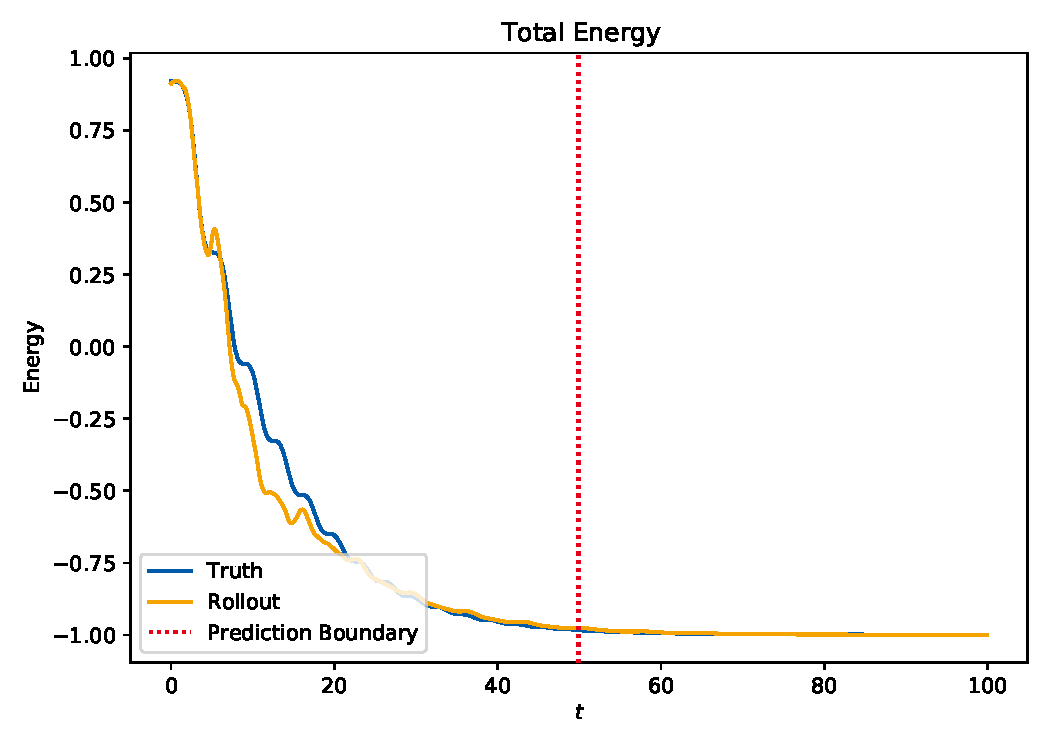
\includegraphics[width=\linewidth]{figures/results/pendulum-damped/run-latent-dim-10/energy-R110-N0-total.png}
			\end{subfigure} \\
			\begin{subfigure}{0.5\linewidth}
				\centering
				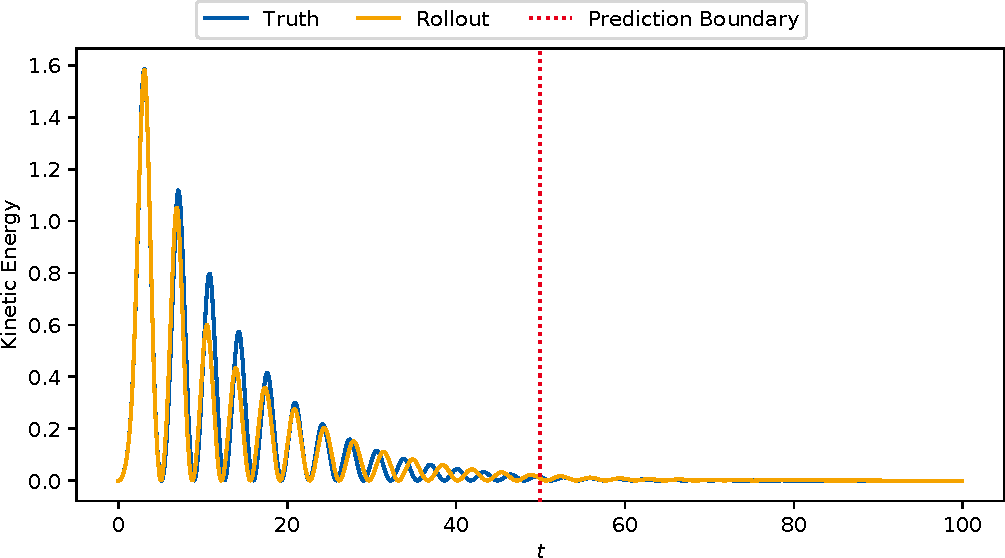
\includegraphics[width=\linewidth]{figures/results/pendulum-damped/run-latent-dim-10/energy-R110-N0-kinetic.png}
			\end{subfigure}%
			~
			\begin{subfigure}{0.5\linewidth}
				\centering
				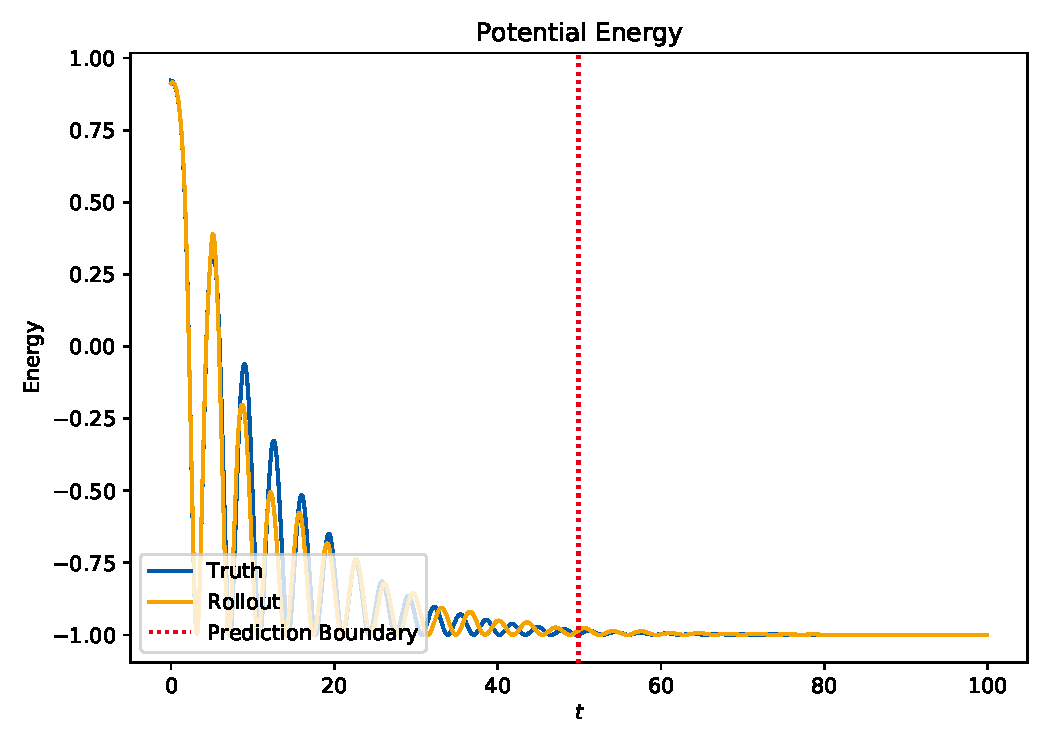
\includegraphics[width=\linewidth]{figures/results/pendulum-damped/run-latent-dim-10/energy-R110-N0-potential.png}
			\end{subfigure}
			\caption[Total energy of the damped pendulum]{Total energy of the damped pendulum composed of the kinetic energy on the bottom left and the potential energy on the bottom right. The blue line represents the true energy, calculated from the training and validation data. The orange line is the energy calculated from the rollout. As usual, the red line is the prediction boundary up until all training data was used; afterwards, the model predicted the rest of the data.}
			\label{fig:pendulumDampedEnergyL10}
		\end{figure}

		\begin{figure}
			\centering
			\includegraphics[width=\linewidth]{figures/results/pendulum-damped/run-latent-dim-10/rollout-latents-N0.png}
			\caption[Latent rollout of the damped pendulum experiment for 10 latent dimensions]{Rollout of the latent dimensions of the damped pendulum environment for \(k = 10 \) latents.}
			\label{fig:pendulumDampedLatentRolloutL10}
		\end{figure}
	% end

	\subsection{Gym Pendulum}
		\label{subsec:discussGymPendulum}

		As we have seen in the experiment with different latent dimensionalities in~\autoref{subsubsec:gymPendulumLatents}, we need at least seven latent dimensions to get a decent \ac{nrmse} on the training rollout. However, we noticed that we get better results in one run for four latent dimensions (see~\autoref{subsubsec:gymPendulumL04}) which we looked at for a comparison with~\cite{mortonDeepVariationalKoopman2019a}. This shows that our algorithm is extremely sensitive to the initialization as the neural network is initialized randomly. Looking at the rollout of the seven-dimensional latent run in~\autoref{subsubsec:gymPendulumL07}, we see that the latent "stops to change" after the prediction boundary in comparison to the four-dimensional latent where the rollout still moves (and roughly captures the dynamics). By taking a look at the rollout in the latent space in~\autoref{fig:gymPendulumLatentRolloutL04} and~\autoref{fig:gymPendulumLatentRolloutL07} for the four- and seven-dimensional run, we see completely different time behaviors.

		As we have already outlined in~\autoref{subsec:discussDampedPendulum}, it is hard for a linear system to be stable when not converging to zero. We see such a behavior in the latent rollout: While the latents of the four-dimensional run all rise exponentially after the prediction horizon, causing movement in the observation space, approximately half of the latents in the seven-dimensional exponentially increase while the other half decreases exponentially. This seems to lead to vanishing within the neural network, explaining the non-movement in the observation space. This behavior might be improved by regularizing the latent dynamics to a system with eigenvalues really close to one, leading to more stable dynamics. Another idea would be to make the latent dynamics time-dependent so compensate for the exploding states by adding an extra latent state just representing the time step. However, this would impose other difficulties and would make the system non-autonomous.

		Another interesting result of the Gym pendulum experiment is that it performs a lot worse than the simple angular pendulum in~\autoref{subsec:discussPendulum}. This might be caused by the sine/cosine terms as these add more nonlinearity to the system (with small angle approximations it is possible to model the pendulum for small displacements, this is not possible using the sine/cosine of the angle). But as taking the sine/cosine of the angle is actually a nonlinear feature transformation typically used to implicitly encode the symmetries in a polar coordinate environment like the pendulum (swinging the pendulum around one time does not increase the angle by \(2\pi\), instead the pendulum works like a congruence class generalized to \(\R\)), we could use the inverse feature transformation to recover the angle from the sine/cosine data and get a similar performance as for the angular pendulum.

		\begin{figure}
			\centering
			\includegraphics[width=\linewidth]{figures/results/pendulum-gym/run-latent-dim-04/rollout-latents-N0.png}
			\caption[Latent rollout of the Gym pendulum experiment for 6 latent dimensions]{Rollout of the latent dimensions of the Gym pendulum environment for \( k = 6 \) latents.}
			\label{fig:gymPendulumLatentRolloutL04}
		\end{figure}
		\begin{figure}
			\centering
			\includegraphics[width=\linewidth]{figures/results/pendulum-gym/run-latent-dim-07/rollout-latents-N0.png}
			\caption[Latent rollout of the Gym pendulum experiment for 7 latent dimensions]{Rollout of the latent dimensions of the Gym pendulum environment for \( k = 7 \) latents.}
			\label{fig:gymPendulumLatentRolloutL07}
		\end{figure}
	% end

	\subsection{Gym Cartpole}
		As we have seen in the experiments with different latent dimensionalities in~\autoref{subsubsec:cartpoleLatents}, we need at least ten latent dimensions to get a decent \ac{nrmse} on the (training) rollout. We have also seen that more latent dimensions (\eg 16 dimensions in~\autoref{subsubsec:cartpoleL16}) do not yield better results than ten latent dimensions (see~\autoref{subsubsec:cartpoleL10}). However, in both cases we get a near-to-perfect rollout before the prediction boundary but fail at the prediction. For the ten dimensional latent, the model captures the dynamics of the pole displacement/velocity and also the cart velocity after the prediction boundary roughly, but for the cart position the trajectory is quite off. Another interesting result is that the model is a lot more confident in the pole displacement and velocity than the cart position. Looking at just the data in~\autoref{fig:envCartpoleGym}, this makes sense. The movement of the car is more complex as it accelerates nonlinearly only through the movement of the pendulum. This does not impose a linear movement on the cart, but rather it is centered around zero with a light shifting occurring when the pendulum falls down or swings up\footnote{See \href{https://github.com/fdamken/bachelors-thesis/blob/b5a4acbc1d10fa0224a73201995222690d2fb6de/thesis/figures/cartpole.gif}{GitHub} for a GIF of the cartpole movement.}. Also, as we have seen in~\autoref{subsec:discussPendulum} and~\autoref{subsec:discussDampedPendulum}, we are able to learn the movement of an undamped and a damped pendulum, where the motion of the pole on a cart can be seen as a slightly damped pendulum as the system is transferring energy from the pendulum to the cart.
	% end

	\subsection{Gym Double Pendulum}
		As we have seen in the experiment with different latent dimensionalities, we need at least 18 latent dimensions to model the double pendulum adequately in the training rollout. As expected from the \ac{nrmse}, we get a decent fit on the rollout for 18 latent dimensions (see~\autoref{fig:acrobotRolloutL18}), but the prediction is far off the true trajectory. The prediction does not even capture the dynamics roughly and also it is pretty certain on its wrong trajectory. This matches our expectations as the double pendulum is a chaotic environment with nonlinear coupling that is really hard to learn.

		Improving the performance on the double pendulum might be possible by using a shorter integration interval \(h\) to provide the algorithm more information between the states such that it can better extrapolate from the data. Another idea, similar to the one outlined in~\autoref{subsec:discussGymPendulum}, would be to apply an inverse feature transform on the sine/cosine of the angles to reduce the dimensionality of the observation space and let "the model discover the symmetries". We will discuss this again in~\nameref{sec:futureWork}. But overall we are satisfied that we managed to learn at least the rollout on the training data even in a chaotic system.
	% end

	\subsection{Running on the CPU or GPU Makes a Difference}
		\label{subsec:cpuGpu}

		We noticed that running our code on the \ac{cpu} or on the \ac{gpu} makes a huge difference in the quality of the results, where running on the \ac{gpu} is better. The environment we noticed the greatest difference is the double pendulum, of which we added two plots in~\autoref{app:plotsCpuGpu}.~\autoref{fig:cpuVsGpuCpu} shows the double pendulum experiment result running on the \ac{cpu} and~\autoref{fig:cpuVsGpuGpu} shows the double pendulum experiment result running on the \ac{gpu}. We expect both plots to be the same, but in fact the plot of the experiment running on the \ac{cpu} looks better. These runs are the runs \texttt{1564} and \texttt{1565}, respectively. In both cases we set the seed for both NumPy and PyTorch to the same value. As the data was generated beforehand, the Gym seed does not matter in this case. We expect this to be an issue with a gradient flowing too far through the computation graph or an issue with floating point operations working differently on the \ac{cpu}/\ac{gpu}.
	% end

	\subsection{Learning Multiple Sequences at Once}
		\label{subsec:singleMulti}

		We derived the Koopman inference algorithm in a way such that it should be possible to learn on multiple observation sequences at once (see~\autoref{sec:ngkDerivation}). However, we noticed that the results of learning from multiple sequences at once yields worse results than learning one observation sequence. We have multiple explanations for this issue, the most probable being an error in the implementation we did not find. Another explanation is that in the single-sequence case the neural network of the observation function overfits to the training data and does not have enough "memory" to also overfit to another observation sequence and therefore breaks. This is a serious problem to address and we might be able to overcome this problem by adding noise to the input to improve generalization.

		\autoref{fig:plotsSingleSequence} and~\autoref{fig:plotsMultiSequence} show two rollouts on the damped pendulum environment, the former only learning on a single observation sequence and the latter learning on multiple sequences at once. We see that while the result of a single sequence captures the dynamics decently (see~\autoref{subsec:discussDampedPendulum} for an in-depth discussion), the model that learned on two sequences does not capture the dynamics correctly.
	% end

	\subsection{Discussion on Numerical Stability}
		\label{subsec:discussPerformanceNumerics}

		The primary thing we noticed in terms of numerical stability is the definiteness of the covariance matrices \(\mat{Q}\), \(\mat{R}\) and \(\mat{V}_0\). While this can be fixed by learning the Cholesky decomposition directly, better regularization or putting priors on the matrices (see~\autoref{sec:futureWork} for more information on these topics), we also faced singular matrices. This primarily happened for high latent dimensionalities, a phenomenon that can also be seen in the latent dimensionalities comparison plots in~\autoref{sec:results}. This is caused by the algorithm "not knowing what to do" with a latent dimension, \ie when it already has "enough" dimensions to explain the data. We could use this behavior to automatically detect which latents are important and which are not, called \emph{automatic relevance determination} (see~\autoref{subsec:ard}) for more proposals on this topic.

		With implementing the square-root filtering/smoothing in the E-step we gained a lot of numerical stability (also also speed) by not having to compute the Cholesky decomposition of every smoothed covariance.

		With all that combined, we are satisfied with the numerical stability of the Koopman inference algorithm, especially given that one of the great instabilities, singular matrices, lead to future work on automatic relevance determination.
	% end
% end

\section{Comparison with Related Work}
	In this section we will discuss the performance of the Koopman inference algorithm in the context of the results from related work, the \ac{dvk} model proposed in~\cite{mortonDeepVariationalKoopman2019a}. We used the code Morton et al. originally published along with their paper and modified it to work with the latest TensorFlow~\cite{abadiTensorFlowLargeScaleMachine2016} and applied the changes mentioned in~\cite{mortonDeepVariationalKoopman2019a} (\ie made the actions of the acrobot and cartpole environment continuous). Additionally, we removed the actuation abilities of the environments along with the control inputs to mimic the behavior of our work which currently does not work with control inputs. Our modified version can be found on GitHub\footnote{See \hrefGithubVariationalKoopman{\texttt{https://github.com/fdamken/variational-koopman}} on the branch \texttt{without-control}.}.

	We ran four different environments:
	\begin{itemize}
		\item The acrobot environment that equals our double pendulum environment presented in~\autoref{subsubsec:doublePendulum}.
		\item Two cartpole environments, one equal to our cartpole environment presented in~\autoref{subsubsec:cartpole} and one with sine and cosine of the pole angle displacement as it was done initially in the \ac{dvk} reference implementation.
		\item The pendulum environment that equals our Gym pendulum environment presented in~\autoref{subsubsec:gymPendulum} with sine/cosine features.
	\end{itemize}
	If possible, we set the number of time steps for training their model equal to the number of time steps we used for training our model. However, due to numerical instabilities in their implementation, we had to deviate in terms of the number of time steps for some environments\footnote{The exact parameters we ran their code with can be found in the \hrefGithubVariationalKoopman{GitHub repository}.}:
	\begin{itemize}
		\item We could only use 32 steps on the cartpole as opposed to ours which used 150.
		\item We used 64 steps on the double pendulum as opposed to ours which uses only 56.
	\end{itemize}
	Also, our algorithm currently only learns on one observation sequence, \ie if we learn on a sequence that covers \(T_\text{train}\) time steps, we only use \(T_\text{train}\) data points, while the \ac{dvk} model uses \num{3968} equally sized sequences. This sums up to \num{253952} data points for the acrobot environment, \num{126976} for the cartpole environment and \num{198400} for the pendulum environment.

	We assess the performance of both models by looking at the rollout plots and evaluating the performance qualitatively, and by comparing the \acrlong{nrmse}. We compute the \ac{nrmse} along the whole trajectory, although we should note that the "rollout" of \ac{dvk} is not a complete rollout as the observations on the training data are reconstructions of the learning data. That is, the rollout starts from the prediction boundary, possibly yielding better results before the boundary as if the data would be computed from the beginning. But this does most probably not affect our assessment in meaningful ways.

	We will now discuss the qualitative performance on each environment separately and afterwards assess the quantitative results for all environments at once.

	\subsection{Pendulum}
		The rollout on the pendulum environment of the \ac{dvk} model is shown in~\autoref{fig:mortonPendulum}. We compare these results with both our results for the Gym pendulum (with sine/cosine) features and our results on the angular pendulum. As discussed in~\autoref{subsec:discussGymPendulum}, we can assume an inverse feature transformation back to the polar coordinate space.

		We see that the reconstruction before the prediction boundary works quite well, however, the sine feature of the angle has a dent around \( t \approx 25 \). In comparison to our rollout in~\autoref{fig:gymPendulumRolloutL04} (on the Gym pendulum), our rollout in the training error before the prediction boundary matches the data better. However, the prediction of the \ac{dvk} model captures the behavior of the system better than our prediction. Looking at the angular pendulum in~\autoref{fig:pendulumRolloutL10} (on ten latent dimensions), our model captures both the dynamics before and after the prediction boundary better than the \ac{dvk} model.

		\begin{figure}
			\centering
			\includegraphics[width=\linewidth]{figures/discussion/morton/pendulum/morton-predictions.png}
			\caption[Rollout of the pendulum environment of the DVK model]{Rollout of the pendulum environment of the \ac{dvk} model, generated by us. The top row shows the sine/cosine of the displacement of the pendulum, the bottom plot shows the angular velocity. The black dots show the ground truth of the trajectory, the solid blue line the reconstructed states from the latents, the dashed blue line the prediction of the model and the shaded region shows the min-to-max distance. This is generated by sampling multiple sequences from the model and taking the maximal and minimal values at each time step. This can be roughly interpreted as the model confidence. The blue line is the mean of the sampled predictions. As usual, the red line is the prediction boundary up until the blue line represents the reconstruction; afterwards, the model predicted the rest of the data.}
			\label{fig:mortonPendulum}
		\end{figure}
	% end

	\subsection{Cartpole}
		For the cartpole environment, we now have two versions of the environment for the \ac{dvk} model: One that uses the angle of the pole displacement directly with the rollout in~\autoref{fig:mortonCartpoleAngle} and one that uses sine/cosine features of the angle in~\autoref{fig:mortonCartpoleSineCosine}.

		We see that both the reconstruction and the prediction for both cases are far away from the true data. Interestingly, in case of the sine/cosine features, the prediction is further away from the true data compared to the angular features, even though the former was a modification originally done in the \ac{dvk} model. But we must note that we were not able to fully reproduce the original results, so the original version might have yielded better results. Compared to our result in~\autoref{fig:cartpoleRolloutL10} (on ten latent dimensions), our model captures the dynamics a lot more accurate in the training section, but worse after the boundary (\ie for prediction), especially in the cart position and velocity. Overall, we can say from this qualitative comparisons, that our model performs better on the cartpole\footnote{Note that we used more time steps for training our model, but overall less data points. Also we were not able to train the \ac{dvk} model on more time steps as it became numerically unstable.}.

		\begin{figure}
			\centering
			\includegraphics[width=\linewidth]{figures/discussion/morton/cartpole/morton-predictions.png}
			\caption[Rollout of the cartpole environment of the \ac{dvk} model with angular features]{Rollout of the cartpole environment of the \ac{dvk} model with angular features, generated by us. The top row shows the position/velocity of the cart, the bottom row shows the angle and angular velocity of the pole one the cart. The black dots show the ground truth of the trajectory, the solid blue line the reconstructed states from the latents, the dashed blue line the prediction of the model and the shaded region shows the min-to-max distance. This is generated by sampling multiple sequences from the model and taking the maximal and minimal values at each time step. This can be roughly interpreted as the model confidence. The blue line is the mean of the sampled predictions. As usual, the red line is the prediction boundary up until the blue line represents the reconstruction; afterwards, the model predicted the rest of the data.}
			\label{fig:mortonCartpoleAngle}
		\end{figure}
		\begin{figure}
			\centering
			\includegraphics[width=\linewidth]{figures/discussion/morton/cartpole-sinecosine/morton-predictions.png}
			\caption[Rollout of the cartpole environment of the \ac{dvk} model with sine/cosine features]{Rollout of the cartpole environment of the \ac{dvk} model with angular features, generated by us. The top row shows the position/velocity of the cart, the middle row shows the cosine/sine of displacement and the bottom row shows the angular velocity of the pole on the cart. The black dots show the ground truth of the trajectory, the solid blue line the reconstructed states from the latents, the dashed blue line the prediction of the model and the shaded region shows the min-to-max distance. This is generated by sampling multiple sequences from the model and taking the maximal and minimal values at each time step. This can be roughly interpreted as the model confidence. The blue line is the mean of the sampled predictions. As usual, the red line is the prediction boundary up until the blue line represents the reconstruction; afterwards, the model predicted the rest of the data.}
			\label{fig:mortonCartpoleSineCosine}
		\end{figure}
	% end

	\subsection{Double Pendulum}
		The final environment we benchmarked on the \ac{dvk} model is the double pendulum, for which both we and the \ac{dvk} model used cosine/sine feature transformations. The rollout of the \ac{dvk} model is shown in~\autoref{fig:mortonAcrobot}.

		We see that the reconstruction and prediction of the angular velocity is quite accurate as well as the reconstruction and prediction of the sine of both angles. However, the cosine only matches some of the data points. Compared to our rollout in~\autoref{fig:acrobotRolloutL18} (on 18 latent dimensions), the reconstruction is worse but the prediction is a lot more accurate than ours on every dimension.

		\begin{figure}
			\centering
			\includegraphics[width=\linewidth]{figures/discussion/morton/acrobot/morton-predictions.png}
			\caption[Rollout of the double pendulum environment of the \ac{dvk} model]{Rollout of the double pendulum environment of the \ac{dvk}, generated by us. The top row shows the cosine/sine of the displacement of the inner pendulum, the middle row shows the cosine/sine of the displacement of the outer pendulum and the bottom row shows the angular velocities of the inner and outer pendulum, from left to right. The black dots show the ground truth of the trajectory, the solid blue line the reconstructed states from the latents, the dashed blue line the prediction of the model and the shaded region shows the min-to-max distance. This is generated by sampling multiple sequences from the model and taking the maximal and minimal values at each time step. This can be roughly interpreted as the model confidence. The blue line is the mean of the sampled predictions. As usual, the red line is the prediction boundary up until the blue line represents the reconstruction; afterwards, the model predicted the rest of the data.}
			\label{fig:mortonAcrobot}
		\end{figure}
	% end

	\subsection{Quantitative Comparison and Summary}
		We now look at a quantitative comparison of both models, the \ac{dvk} model and the Koopman inference algorithm (ours). We use the \ac{nrmse} on the complete rollout, the rollout on the training data (or, in case of \ac{dvk}, the reconstruction) and the prediction. We summarized the different errors in~\autoref{tab:mortonComparison}, where our algorithm is almost consistently better at environments that use the angle directly instead of the cosine/sine. Also, we are almost always better in terms of the training rollout, while we perform worse in the prediction. However, these numbers should be taken with care as the \ac{nrmse} is not scale-independent (even though it is better than the \ac{rmse} due to the normalization), but as the errors reflect our results from the qualitative comparison, we are confident that our algorithm performs better.

		Overall we are satisfied with the performance of our algorithm compared to the \ac{dvk} Koopman model for multiple reasons: Firstly, we gauge the uncertainty directly instead of sampling multiple trajectories and treating the min-max distance as uncertainty. Secondly, our algorithm is much more sample-efficient (see the numbers at the beginning of this section). Thirdly, as already mentioned in related work, our method has a lot simpler model in terms of number of parameters and number of neural networks.

		\begin{table}
			\centering
			\begin{tabular}{c|c|c|c}
				    \textbf{Environment}      & \textbf{Error on}\dots & \textbf{Deep Variational Koopman} & \textbf{Koopman Inference} \\ \hline
				\textbf{Sine/Cosine Pendulum} &        Complete        &               0.198               &       \textbf{0.023}       \\
				        \textbf{vs.}          &        Training        &               0.168               &       \textbf{0.014}       \\
				  \textbf{Angular Pendulum}   &       Prediction       &               0.222               &       \textbf{0.029}       \\ \hline
				\textbf{Sine/Cosine Pendulum} &        Complete        &          \textbf{0.198}           &           0.200            \\
				        \textbf{vs.}          &        Training        &               0.168               &       \textbf{0.003}       \\
				\textbf{Sine/Cosine Pendulum} &       Prediction       &          \textbf{0.222}           &           0.282            \\ \hline
				  \textbf{Angular Cartpole}   &        Complete        &               0.265               &       \textbf{0.200}       \\
				        \textbf{vs.}          &        Training        &               0.466               &       \textbf{0.009}       \\
				  \textbf{Angular Cartpole}   &       Prediction       &               0.420               &       \textbf{0.377}       \\ \hline
				\textbf{Sine/Cosine Cartpole} &        Complete        &               0.470               &       \textbf{0.200}       \\
				        \textbf{vs.}          &        Training        &              17.222               &       \textbf{0.009}       \\
				  \textbf{Angular Cartpole}   &       Prediction       &               0.817               &       \textbf{0.377}       \\ \hline
				                              &        Complete        &          \textbf{0.102}           &           0.228            \\
				  \textbf{Double Pendulum}    &        Training        &               0.103               &       \textbf{0.002}       \\
				                              &       Prediction       &          \textbf{0.104}           &           0.562
			\end{tabular}
			\caption{Errors of all environments we benchmarked DVK and Koopman inference on. The environment in the first column describes which environment the data of the DVK is collected from (before "vs.") and from which environment the data of the Koopman inference algorithm is collected from (after "vs."). The complete error is over the rollout/reconstruction over the whole sequence, the training error is over the rollout/reconstruction on the training data and prediction is over rollout on the validation data. The numbers represent the NRMSE. The respective lowest error is marked in bold.}
			\label{tab:mortonComparison}
		\end{table}
	% end
% end

%\section{Control}  % Only if there is time left!
%	% Introduce approach to control.
%	% Show results of LGDS control which is working.
%	% Highlight difficulties.
%
%	\todo{Discussion: Control}
%% end

\section{Future Work}
	\label{sec:futureWork}

	We will now discuss and propose future work and ideas that can be tried based on the results of this thesis.

	\subsection{Control}
		In this thesis we presented a method for learning a dynamical system with no control inputs. The most obvious extension would be to add control inputs to the latent space in an additive fashion \( \vec{s}_{t + 1} = \mat{A} \vec{s}_t + \mat{B} \vec{u}_t \) with a learnable control matrix \(\mat{B}\). With this approach it might be possible to actually perform \ac{mpc} and uncertainty-aware control like in~\cite{mortonDeepVariationalKoopman2019a}, but with a simpler model. Our first approach to this would be to test this method on a simple environment like the pendulum and first learn the control rollout and afterwards perform a stabilization task and try the swing-up of the pendulum.
	% end

	\subsection{Bayesian Treatment}
		Another extension would be to employ a Bayesian view on the parameters and treat \eg the state dynamics matrix, covariance matrices and so on as random variables. This would allow to gauge the uncertainty on the dynamics itself and would allow to restrict the matrices to small ones by placing a prior on them. The approach would be to remove the \ac{ml} estimator and marginalize over the parameters to get a predictive distribution. Another semi-Bayesian approach would be to use point-estimates using a \ac{map} estimator rather than a predictive distribution.
	% end

	\subsection{Automatic Relevance Determination (ARD)}
		\label{subsec:ard}

		In combination with going full Bayesian on the model goes the implementation of automatic relevance determination of latent dimensions as proposed in~\cite{bealVariationalKalmanSmoother2000} for linear systems. Choosing a zero-mean prior might lead to a determination of non-relevant latent states, driving the state dynamics matrix to zero. Implementing this could solve the problems described in~\autoref{subsec:discussPerformanceNumerics} that the algorithm does already have "enough" latent dimensions and drives the variance to a high level on some dimensions.
	% end

	\subsection{Better Regularization and Learning the Cholesky Decomposition}
		As already outlined in~\autoref{subsubsec:implRegularization}, it might be beneficial for numerical stability to directly learn the Cholesky decomposition of the covariance matrices by using numerical optimization instead of closed-form optimization. Another approach could be to impose better regularization on the matrices if they become negative (semi-) determinant. However, while giving this a short first try during our implementation, we found out that just adding some values to the diagonal does not lead to better model performance but rather drives the likelihood to negative infinity.
	% end

	\subsection{Speed Improvements by Full PyTorch or Enhanced QR Decomposition}
		As the square-root smoothing heavily uses QR decompositions which are faster on the CPU but the M-step uses backpropagation which is faster on the GPU, we had to copy the data over in every \ac{em} iteration. It might be beneficial to implement a more advanced QR decomposition (\eg~\cite{andersonCommunicationAvoidingQRDecomposition2011a}) and run the whole algorithm in the GPU.
	% end

	\subsection{(Inverse) Feature Transformations}
		As we have seen in~\autoref{subsec:discussGymPendulum} and~\ref{subsec:discussPendulum}, using the angle directly instead of the sine/cosine improves prediction abilities a lot. It might be beneficial to try out the proposed inverse feature transformation to get the angle back from sine and cosine and to apply this technique to other environments as well (\eg the double pendulum).
	% end
% end

	\chapter{Conclusion}
\label{c:conclusion}



Linearization is very important in control to handle nonlinear systems that exhibit complicated dynamics. We have looked at Koopman theory, a technique to find globally linear embedding for a nonlinear system. Unfortunately, the Koopman operator, the core of Koopman theory, is generally infinite-dimensional. Prior work~\cite{bruntonKoopmanInvariantSubspaces2016,kaiserDatadrivenDiscoveryKoopman2020,luschDeepLearningUniversal2018} has shown that we can find a finite-dimensional representation of the operator. These representations seek Koopman eigenfunctions that span an invariant subspace of the embedding and do not transform under the influence of the Koopman operator other than being scaled. Nevertheless, most of the existing approaches work on deterministic models, seeking the Koopman eigenfunctions. While methods have been proposed to take a probabilistic perspective on the Koopman operator, these methods use complicated model setups with multiple neural networks and do not directly gauge the uncertainty of model predictions.

We have combined existing theory for \acl{lgds} with cubature rules to approximate arising nonlinear Gaussian integrals in a deterministic way to build up an \acl{em} algorithm. We called the result algorithm the \emph{Koopman inference} algorithm. It is alternating between estimating the states in the E-step and optimizing the linear latent state dynamics and a nonlinear observation function that maps the linear latent states back to the nonlinear dynamics. This way, we were able to predict the nonlinear dynamics and learned the Koopman observation functions without hand-tuned loss functions like in~\cite{luschDeepLearningUniversal2018}.

We evaluated the model performance on multiple different environments: A simple pendulum, a damped pendulum, the cartpole environment and a double pendulum. We used two different approaches for learning the dynamics of the pendulum, one of which uses sine/cosine feature transformations of the pendulum displacement and one that learn the angle directly. We also proved and showed empirically that our algorithm extends the common algorithm for learning \ac{lgds} by showing that the used  integral approximations are exact for linear functions and validating the result on a regular \ac{lgds}. We have found out that learning systems that lose energy (\eg the damped pendulum) are generally easier to learn as systems that conserve energy (\eg the undamped pendulum), as the the latent dynamics have to be stable but not attract zero to keep moving. Additionally, we discovered that the pendulum with sine/cosine features is a lot harder to learn, presumably because of the additional nonlinearity added by the feature transformation. Also, we roughly learned the dynamics of the double pendulum environment, even though this is a chaotic system and we were not able to predict further movements beyond the training data.

Finally, we compared our Koopman inference algorithm against the \acl{dvk} model proposed by~\cite{mortonDeepVariationalKoopman2019a}. We saw that our algorithm performs similar, however, the \ac{dvk} model is better in predicting the dynamics beyond the training data, while we are primarily able to predict until the end of the training data. We should note that the \ac{dvk} performs reconstruction from the latents that were learned during the training while our model performs the rollout from the beginning.

Overall we are satisfied with the performance of the Koopman inference algorithm and it allows for further improvements of learning the influence of control inputs on actuated systems or employing a Bayesian view on the latent dimensions and further gauge the uncertainty on the state dynamics.


	\cleardoublepage
	\bibliography{literature/lit}

	\cleardoublepage
	\appendix
	\chapter{Full Derivation of the \algname Algorithm}
\label{app:fullNgkDerivation}



\todo{Full Derivation of NGK.}

	\chapter{Miscellaneous}
	\section{Solution of the Harmonic Oscillator}
		\label{app:harmonicOscillatorSolution}

		To solve the differential motion equation
		\begin{align*}
			m\ddot{x} = -kx
		\end{align*}
		of the harmonic oscillator given in~\autoref{subsec:harmonicOscillator}, we use the solution approach
		\begin{align*}
			x(t) = c e^{\lambda t} \qquad \dot{x}(t) = \lambda c e^{\lambda t} \qquad \ddot{x}(t) = \lambda^2 c e^{\lambda t}
		\end{align*}
		and insert it into the differential equation:
		\begin{align*}
			m\ddot{x} = -kx \quad\implies\quad
			m \lambda^2 c e^{\lambda t} = -k c e^{\lambda t} \quad\iff\quad
			m \lambda^2 = -k \quad\iff\quad
			\lambda = \pm \sqrt{-\frac{k}{m}}
		\end{align*}
		As both \(k\) and \(m\) are defined to be positive, we get the complex solutions:
		\begin{align*}
			x_1(t) = e^{i t \sqrt{k / m}} \qquad x_2(t) = e^{-i t \sqrt{k / m}}
		\end{align*}
		Due to the superposition principle, also \( x_1 + x_2 \) and \( x_1 - x_2 \) are solutions. Hence, we get two real solutions by using Euler's identity \( e^{\varphi i} = \cos(\varphi) + i \sin(\varphi) \):
		\begin{align*}
			x_1 + x_2
				&= e^{i t \sqrt{k / m}} + e^{-i t \sqrt{k / m}} \\
				&= \cos\Big(t \sqrt{k / m}\Big) + i \sin\Big(t \sqrt{k / m}\Big) + \cos\Big(t \sqrt{k / m}\Big) - i \sin\Big(t \sqrt{k / m}\Big) \\
				&= 2 \cos\Big(t \sqrt{k / m}\Big) \\
			x_1 - x_2
				&= e^{i \sqrt{k / m} t} - e^{-i t \sqrt{k / m}} \\
				&= \cos\Big(t \sqrt{k / m}\Big) i \sin\Big(t \sqrt{k / m}\Big) - \cos\Big(t \sqrt{k / m}\Big) + i \sin\Big(t \sqrt{k / m}\Big) \\
				&=  2i \sin\Big(t \sqrt{k / m}\Big)
		\end{align*}
		This yields the following general solution:
		\begin{align*}
			x(t) = c_1 \cos\Big(t \sqrt{k / m}\Big) + c_2 \sin\Big(t \sqrt{k / m}\Big),\quad c_1, c_2 \in \C
		\end{align*}
		As both Sine and Cosine are Sinusoidal, different \( c_1 \neq c_2 \) only lead to a phase shift. Thus we can also write the solution as
		\begin{align*}
			x(t) = A \cos\Big(t \sqrt{k / m} + \varphi\Big)
		\end{align*}
		with the amplitude \(A\) and the phase \(\varphi\).
	% end

	\section{Overview over Notations for Linear Gaussian Dynamical Systems}
		\begin{table}[ht]
			\centering
			\begin{tabular}{l|ccc}
				\textbf{Element / Definition} & \textbf{Ghahramani}~\cite{ghahramaniParameterEstimationLinear1996} & \textbf{Minka}~\cite{minkaHiddenMarkovModels1999} & \textbf{This Thesis} \\ \hline
				Time                         & \( t \)                         & \( t \)                 & \( t \)                                                    \\
				Last Timestep                & \( T \)                         & \( T \)                 & \( T \)                                                    \\
				State                        & \( \vec{x}_t \)                 & \( \vec{s}_t \)         & \( \vec{s}_t \)                                            \\
				Observations                 & \( \vec{y}_t \)                 & \( \vec{x}_t \)         & \( \vec{y}_t \)                                            \\
				State Dynamics Matrix        & \( \mat{A} \)                   & \( \mat{A} \)           & \( \mat{A} \)                                              \\
				State Noise Covariance       & \( \mat{Q} \)                   & \( \mat{\Gamma} \)      & \( \mat{Q} \)                                              \\
				Observation Matrix           & \( \mat{C} \)                   & \( \mat{C} \)           & \( \mat{C} \)                                              \\
				Observation Noise Covariance & \( \mat{R} \)                   & \( \mat{\Sigma} \)      & \( \mat{R} \)                                              \\
				Full Sequence \( \big( \vec{x}_1, \vec{x}_2, \cdots, \vec{x}_T \big) \)
				                             & \( \{ \vec{x} \} \)             & \( \vec{x}_{1:T} \)     & \( \vec{x}_{1:T} \)                                        \\
				Subsequence \( \big( \vec{x}_{t_0}, \vec{x}_{t_0 + 1}, \cdots, \vec{x}_{t_1} \big) \)
				                             & \( \{ \vec{x} \}_{t_0}^{t_1} \) & \( \vec{x}_{t_0:t_1} \) & \( \vec{x}_{t_0:t_1} \)                                    \\
				Expected Log Likelihood      & \( Q \)                         & \( Q \)                 & \( Q \)                                                    \\
				Predicted State              & \( \vec{x}_t^{t - 1} \)         & --                      & \( \hat{\vec{s}}_{t \subgiven t - 1} \)                    \\
				Predicted Covariance         & \( \mat{V}_t^{t - 1} \)         & \( \mat{P}_{t - 1} \)   & \( \hat{\mat{V}}_{t \subgiven t - 1} \)                    \\
				Filtered State               & \( \vec{x}_t^t \)               & \( \vec{m}_t \)         & \( \hat{\vec{s}}_{t \subgiven t} \)                        \\
				Filtered Covariance          & \( \mat{V}_t^t \)               & \( \mat{V}_t \)         & \( \hat{\mat{V}}_{t \subgiven t} \)                        \\
				Smoothed State               & \( \hat{\vec{x}}_t \)           & \( \hat{\vec{m}}_t \)   & \( \hat{\vec{s}}_t \), \( \hat{\vec{s}}_{t \subgiven T} \) \\
				Smoothed Covariance          & \( \mat{V}_t^T \)               & \( \hat{\mat{V}}_t \)   & \( \hat{\mat{V}}_t \), \( \hat{\mat{V}}_{t \subgiven T} \) \\
				Self-Correlation \( \E\big[\vec{x}_t \vec{x}_t^T \biggiven \{ \vec{y} \}\big] \)
				                             & \( \mat{P}_t \)                 & --                      & \( \mat{P}_t \)                                            \\
				Cross-Correlation \( \E\big[\vec{x}_t \vec{x}_{t-1}^T \biggiven \{ \vec{y} \}\big] \)
				                             & \( \mat{P}_{t, t - 1} \)        & --                      & \( \mat{P}_{t, t - 1} \)
			\end{tabular}
			\caption[Notations used for linear Gaussian dynamical systems in different papers]{Notations used for linear Gaussian dynamical systems in different papers.}
		\end{table}
	% end

	\section{Framework-Specific Implementation Problems}
		\label{app:implFrameworkProblems}

		\subsubsection{Slow QR Decomposition on GPU}
			During our implementation we found found that QR decomposition is relatively slow on the \ac{gpu} due to a bug in PyTorch\footnote{See \href{https://web.archive.org/web/20201110121407/https://github.com/pytorch/pytorch/issues/22573}{\texttt{https://github.com/pytorch/pytorch/issues/22573}}.} at the time of writing. While faster QR decomposition methods on a \ac{gpu} have been proposed~\cite{andersonCommunicationAvoidingQRDecomposition2011a}, we stuck to copying the data back and forth between \ac{cpu} and \ac{gpu} in every \ac{em} iteration.

			We also address this in~\nameref{sec:futureWork}.
		% end

		\subsubsection{Issues with Numerical Integration}
			\label{subsubsec:integrationProblems}

			We should note that some environments we ran experiments on are described by stiff differential equations, \eg the pendulum or the cartpole environment. As stiff \acp{ode} can not be integrated well with explicit solution methods, implicit methods should be preferred throughout the data generation. For some environments in OpenAI's Gym~\cite{brockmanOpenAIGym2016}, this has to be explicitly configured, \eg for the cartpole environment with \lstinline|env.kinematics_integrator = 'implicit-euler'|. Not changing the integrator leads to catastrophic data. In case of the cartpole, using the explicit Euler method causes the pole to build up energy and to get significantly faster over time.
		% end
	% end
% end

	\chapter{Experiments}
\label{c:experiments}
\IMRADlabel{results}



In this chapter we will present all environments we experimented with as well as \emph{hyper-experiments}, \ie experiments with the hyperparameters and their influence on the algorithm performance (in terms of the prediction error and similar metrics, not the computing time).

We split this chapter into two parts: Firstly, we will present the experiment setup we used and the different environments we tested on. Secondly, we present our results and put them in context of other results. All critical discussion and comparison with related work will take place in~\autoref{c:discussion}.

\section{Setup}
	In this section we will introduce the experiment setup and all the different environments we used for evaluation.

	\subsection{Environments}
		This section covers the different environments we used and changes we have applied to them. Note that we separated the data generation process from running the experiment. For each of the following experiments we include the experiment ID at the beginning that can be used to locate the experiment in the code.

		\subsubsection{Proof-of-Concept: Classic LGDS}
			\begin{itemize}
				\item Experiment ID: \texttt{lgds}
			\end{itemize}

			As a proof-of-concept and to empirically verify our proof on the exactness of the cubature rule and hence the similar expected performance for plain linear systems, we benchmark our algorithm against a simple linear system. The linear system has a two-dimensional state \( \vec{y} \coloneqq \begin{bmatrix} x_1 & x_2 \end{bmatrix}^T \) with the dynamics
			\begin{align*}
				\dot{x}_1 &= x_2 \\
				\dot{x}_2 &= -x_1
			\end{align*}
			The initial state \( \vec{s}_1 \) is sampled from a Gaussian with mean \( \begin{bmatrix} 0.1 & 0.2 \end{bmatrix}^T \) and covariance \( \diag\big(10^{-5}, 10^{-5}\big) \). The system is integrated using the implicit Runge-Kutta Radau~IIA~\cite{guglielmiImplementingRadauIIA2001} method with an evaluation interval of \( h = 0.1 \) for \( T = 240 \) time steps where only the first \( T_\train = 120 \) steps are used for training and the remaining \(120\) are used for validation. The raw data is shown in~\autoref{fig:envLgds}.

			As the system's eigenvalues \( -i \), \( i \) are purely imaginary, the integrated system rings around the equilibrium \( \begin{bmatrix} 0 & 0 \end{bmatrix}^T \) indefinitely.

			\begin{figure}
				\centering
				\includegraphics[width=\linewidth]{figures/experiments/environments/observations-lgds-N0.png}
				\caption[Raw data of the proof-of-concept LGDS environment]{Plot of the raw data used for training the proof-of-concept LGDS environment with the first dimension on the left and the second dimension on the right. The black dots represent the actual data points, all before the red prediction boundary are used for training, the rest for validation. The faint gray line emphasizes the connection between the data points and that they are actually generated from a dynamical system.}
				\label{fig:envLgds}
			\end{figure}
		% end

		\subsubsection{(Damped) Pendulum}
			\begin{itemize}
				\item Experiment ID: \texttt{pendulum} and \texttt{pendulum\_damped}
			\end{itemize}

			The first nonlinear system we look at is the (inverted) pendulum in both an undamped and a damped setting. For this experiment, we use the angular state \( \vec{y} = \begin{bmatrix} \theta & \dot{\theta} \end{bmatrix} \) where \(\theta\) is the displacement angle (see~\autoref{fig:envPendulumSketch}). The dynamics are specified by the \ac{ode}
			\begin{equation*}
				\ddot{\theta} = \sin\theta - d \dot{\theta}
			\end{equation*}
			that is solved using the Radau~IIA~\cite{guglielmiImplementingRadauIIA2001} \ac{ivp} integrator (after transforming the \ac{ode} to a first-order \ac{ode} system). The initial velocity is set to \(0\) and the initial position is sampled from a Gaussian with mean \( \pi/36 \) and variance \( \pi/8 \). This puts the pendulum in motion as it falls down from its initial position. For the undamped pendulum, we set \( d = 0 \). For both environments, we use an evaluation interval of \( h = 0.1 \) for \( T = 1000 \) time steps where only the first \( T_\train = 500 \) steps are used for training and the remaining \(500\) are used for validation. The raw data is shown in~\autoref{fig:envPendulum} for the undamped and~\autoref{fig:envPendulumDamped} for the damped pendulum.

			The damped pendulum is especially interesting as the system looses energy (\ie the sum of the kinetic and potential energy decreases over time) and the embedding has to encode this behavior.

			\begin{figure}
				\centering
				\includegraphics[width=\linewidth]{figures/experiments/environments/observations-pendulum-N0.png}
				\caption[Raw data of the undamped pendulum environment]{Plot of the raw data used for training the undamped pendulum environment. The left plot shows the displacement and the right plot the angular velocity. The black dots represent the actual data points, all before the red prediction boundary are used for training, the rest for validation. The faint gray line emphasizes the connection between the data points and that they are actually generated from a dynamical system.}
				\label{fig:envPendulum}
			\end{figure}
			\begin{figure}
				\centering
				\includegraphics[width=\linewidth]{figures/experiments/environments/observations-pendulum-damped-N0.png}
				\caption[Raw data of the damped pendulum environment]{Plot of the raw data used for training the damped pendulum environment. The left plot shows the displacement and the right plot the angular velocity. The black dots represent the actual data points, all before the red prediction boundary are used for training, the rest for validation. The faint gray line emphasizes the connection between the data points and that they are actually generated from a dynamical system.}
				\label{fig:envPendulumDamped}
			\end{figure}

			\begin{figure}
				\centering
				\tikzSimplePendulum
				\caption[Illustration of the pendulum environment]{Illustration of the pendulum environment. The pendulum has length \(L\) and mass \(m\) and is attached to a fixed point in the center around which it can swing. In the case of the damped pendulum is damped with a damping constant \(d\).}
				\label{fig:envPendulumSketch}
			\end{figure}
		% end

		\subsubsection{Gym Pendulum}
			\begin{itemize}
				\item Experiment ID: \texttt{pendulum\_gym}
			\end{itemize}

			This is a sine/cosine version of the pendulum introduced before, but without damping. We use the environment of OpenAI Gym~\cite{brockmanOpenAIGym2016} for generating the data used for training. The motion equations are still the same as for the non-Gym pendulum
			\begin{equation*}
				\ddot{\theta} = \sin\theta
			\end{equation*}
			with \( d = 0 \) as the Gym pendulum does not include damping, but the state is defined as the sine and cosine of the angle:
			\begin{equation*}
				\vec{y} \coloneqq
					\begin{bmatrix}
						\cos\theta \\
						\sin\theta \\
						\dot{\theta}
					\end{bmatrix}
			\end{equation*}
			The Gym environment uses the Euler method for integrating the \ac{ode} with a step size of \( h = 0.05 \). We generate \( T = 100 \) time steps of which \( T_\train = 50 \) are used for training and the other \(50\) for validation. The raw data is shown in~\autoref{fig:envPendulumGym}.

			\begin{figure}
				\centering
				\includegraphics[width=\linewidth]{figures/experiments/environments/observations-pendulum-gym-N0.png}
				\caption[Raw data of the Gym pendulum environment]{Plot of the raw data used for training the Gym pendulum environment. The top row shows the cosine/sine of the displacement of the pendulum and the bottom plot shows the angular velocity. The black dots represent the actual data points, all before the red prediction boundary are used for training, the rest for validation. The faint gray line emphasizes the connection between the data points and that they are actually generated from a dynamical system.}
				\label{fig:envPendulumGym}
			\end{figure}
		% end

		\subsubsection{Gym Cartpole}
			\label{subsubsec:cartpole}

			\begin{itemize}
				\item Experiment ID: \texttt{cartpole\_gym}
			\end{itemize}

			The second last environment we run experiment on is the cartpole environment. In the cartpole environment, an inverted pendulum is build on a (typically controlled, but otherwise freely movable) cart. If the pendulum falls down, the torque on the joint is translated into a force moving the cart around. This creates nonlinear coupling and therefore, highly nonlinear dynamics. A sketch of the cartpole environment is given in~\autoref{fig:envCartpoleGymSketch}. As for the previous pendulum, we rely on the cartpole implementation of Gym. We slightly modified the environment to be uncontrolled, as the environment usually has discrete actions for pushing the cart left or right. This modification is shown in~\autoref{lst:uncontrolledCartPole}. The state of the environment is given as
			\begin{equation*}
				\vec{y} \coloneqq
					\begin{bmatrix}
						x \\
						\dot{x} \\
						\theta \\
						\dot{\theta}
					\end{bmatrix}
			\end{equation*}
			where \(x\) is the cart position, \(\dot{x}\) is the cart velocity, \(\theta\) is the pole angle and \(\dot{\theta}\) is the angular velocity. The implemented equations of movement, taken from~\cite{florianCorrectEquationsDynamics2005}, are given as:
			\begin{align*}
				\ddot{\theta} &= \frac{g \sin\theta + \cos\theta \Big(\! \frac{-F - m_p \ell \dot{\theta}^2 \sin\theta}{m_c + m_p} \!\Big)}{\ell \Big(\! \frac{4}{3} - \frac{m_p \cos^2\theta}{m_c + m_p} \!\Big)} \\
				\ddot{x} &= \frac{F + m_p \ell \big( \dot{\theta}^2 \sin\theta - \ddot{\theta} \cos\theta \big)}{m_c + m_p}
			\end{align*}
			Here \( g = \SI{9.8}{\meter\per\second\squared} \) is the gravitational acceleration, \( m_p = \SI{0.1}{\kilogram} \) and \( m_c = \SI{1}{\kilogram} \) are the masses of the pole and cart, respectively, \( 2\ell = \SI{1}{\meter} \) is the pole length and \( [F] = \si{\newton} \) is the external (control) force acting on the cart that we set to \( \SI{0}{\newton} \). The Gym environment uses an implicit Euler method\footnote{As mentioned in~\autoref{subsubsec:integrationProblems}, this has to be set manually with \lstinline|env.kinematics_integrator = 'implicit-euler'|.} for integrating the \ac{ode} with a step size of \( h = 0.02 \). We generate \( T = 300 \) time steps of which we use \( T_\train = 150 \) for training and the remaining \(150\) steps for validation. The raw data is shown in~\autoref{fig:envCartpoleGym}.

			\begin{lstlisting}[caption={[Modification of Gym's cartpole environment to get an uncontrolled cartpole]Modification of Gym's cartpole environment to get an uncontrolled cartpole.}, label=lst:uncontrolledCartPole]
from gym.envs.classic_control import CartPoleEnv

class UncontrolledCartPole(CartPoleEnv):
	def __init__(self):
	super().__init__()

	self.force_mag = 0.0
			\end{lstlisting}

			\begin{figure}
				\centering
				\tikzCartpole
				\caption[Illustration of the cartpole environment]{Illustration of the cartpole environment. The cart has mass \(m_c\), the pole \(m_p\) with length \(L\). The cart can move freely on the \(x\) axis, while the pendulum can swing freely around the center of the cart, causing the cart to move.}
				\label{fig:envCartpoleGymSketch}
			\end{figure}

			\begin{figure}
				\centering
				\includegraphics[width=\linewidth]{figures/experiments/environments/observations-cartpole-gym-N0.png}
				\caption[Raw data of the cartpole environment]{Plot of the raw data used for training the Gym cartpole environment. The top plot is the cart position (left) and velocity (right), the row the pole displacement (left) and angular velocity (right). The black dots represent the actual data points, all before the red prediction boundary are used for training, the rest for validation. The faint gray line emphasizes the connection between the data points and that they are actually generated from a dynamical system.}
				\label{fig:envCartpoleGym}
			\end{figure}
		% end

		\subsubsection{Gym Double Pendulum}
			\label{subsubsec:doublePendulum}

			\begin{itemize}
				\item Experiment ID: \texttt{acrobot\_gym}
			\end{itemize}

			The last environment we test on is the double pendulum, implemented in Gym as the \emph{acrobot} (as for the cartpole, we removed all control inputs and modified the initial state to start on top rather than hanging straight down, see~\autoref{lst:topAcrobot}). The double pendulum consists of a pendulum on a fixed joint and a second pendulum attached to the end of the first pendulum. This creates highly nonlinear coupling and is the most common example of a chaotic system~\cite{shinbrotChaosDoublePendulum1992}. We observe the state vector
			\begin{equation*}
				\vec{y} \coloneqq
					\begin{bmatrix}
						\cos\varphi_1 \\
						\sin\varphi_1 \\
						\cos\varphi_2 \\
						\sin\varphi_2 \\
						\dot{\varphi}_1 \\
						\dot{\varphi}_2
					\end{bmatrix}
			\end{equation*}
			where \(\varphi_1\) and \(\varphi_2\) are the displacement of the first and second joint, respectively. See~\autoref{fig:envDoublePendulumGymSketch} for a sketch of the double pendulum. The governing equations of motion are given as:
			\begin{align*}
				\ddot{\varphi}_1 &= \frac{g (\sin\varphi_2 \, \cos\varphi_\Delta - \mu \sin\varphi_1) - (\ell_2 \dot{\varphi}_2^2 + \ell_1 \dot{\varphi}_1^2 \cos\varphi_\Delta) \sin\varphi_\Delta}{\ell_1 (\mu - \cos^2\varphi_\Delta)} \\
				\ddot{\varphi}_2 &= \frac{g \mu (\sin\varphi_2 \, \cos\varphi_\Delta - \mu \sin\varphi_1) + (\mu \ell_1 \dot{\varphi}_1^2 + \ell_2 \dot{\varphi}_2^2 \cos\varphi_\Delta) \sin\varphi_\Delta}{\ell_2 (\mu - \cos^2\varphi_\Delta)}
			\end{align*}
			with \( \varphi_\Delta \coloneqq \varphi_1 - \varphi \), \( \mu \coloneqq 1 + m_1/m_2 \) where \( g = \SI{9.8}{\meter\per\second\squared} \) is the gravitational acceleration, \( m_1 = \SI{1}{\kilogram} \) and \( m_2 = \SI{1}{\kilogram} \) are the masses of the two links and \( \ell_1 = \SI{1}{\meter} \) and \( \ell_2 = \SI{1}{\meter} \) are the lengths of the two links. The Gym environment uses a \ac{rk4} for integrating the \ac{ode} with an evaluation interval of \( h = 0.2 \). We modified the initial position to be drawn from a Gaussian with mean \( \pi \) and standard deviation \( \pi/8 \) and the initial velocity to be drawn from a uniform distribution in the interval \( [-0.1, 0.1] \). We generate \( T = 100 \) time steps of which we use \( T_\train = 75 \) for training and the remaining \(25\) for validation. The raw data is shown in~\autoref{fig:envDoublePendulumGym}.

			\begin{lstlisting}[caption={[Modification of Gym's acrobot environment to start at the top instead of hanging down]Modification of Gym's acrobot environment to start at the top instead of hanging down.}, label=lst:topAcrobot]
import numpy as np
from gym.envs.classic_control import AcrobotEnv

class ModifiedAcrobotEnv(AcrobotEnv):
	def __init__(self):
		super().__init__()

	def reset(self):
		position = self.np_random.normal(np.pi, np.pi / 8.0, size=(2,))
		velocity = self.np_random.uniform(low=-0.1, high=0.1, size=(2,))
		self.state = np.concatenate([position, velocity], axis=0)
		return self._get_ob()
			\end{lstlisting}

			\begin{figure}
				\centering
				\tikzDoublePendulum
				\caption[Illustration of the double pendulum environment]{Illustration of the double pendulum environment. The pendulums have lengths \(\ell_1\) and \(\ell_2\) with the masses \(m_1\) and \(m_2\) attached to the respective ends. The inner pendulum can swing freely around the center while the other pendulum can swing freely around the end of the inner pendulum. Hence, fixing one of the pendulums would transform the system back to a simple pendulum. If both pendulums can swing, the system is chaotic.}
				\label{fig:envDoublePendulumGymSketch}
			\end{figure}

			\begin{figure}
				\centering
				\includegraphics[width=\linewidth]{figures/experiments/environments/observations-acrobot-gym-N0.png}
				\caption[Raw data of the double pendulum environment]{Plot of the raw data used for training the Gym double pendulum environment. The top row shows the cosine/sine of the displacement of the inner pendulum, the middle row shows the cosine/sine of the displacement of the outer pendulum and the bottom row shows the angular velocity of the inner and outer pendulum. The black dots represent the actual data points, all before the red prediction boundary are used for training, the rest for validation. The faint gray line emphasizes the connection between the data points and that they are actually generated from a dynamical system.}
				\label{fig:envDoublePendulumGym}
			\end{figure}
		% end
	% end

	\subsection{Experiment Setup}
		\label{subsec:experimentSetup}

		We now introduce the experiment setup and initialization we used for each environment. For all experiments, we initialized the latent state dynamics matrix \( \mat{A} \) with an identity matrix, the initial state \( \vec{m}_0 \) with a one-vector and all covariance matrices \( \mat{R} \), \( \mat{Q} \) and \( \mat{V}_0 \) with a small diagonal covariance of \( 10^{-5} \). We set the maximum number of \(\vec{g}\)-optimization iterations to \(1000\) for all environments. As described in~\autoref{sec:implementation}, we used a neural network for the observation function with \(\tanh\) activation functions (except for the output layer of course) and a single hidden layer with \(50\) neurons. We used \(100\) maximum iterations for the pendulum, \(200\) for the damped pendulum, \(500\) for the Gym pendulum, \(500\) for the Gym cartpole and \(250\) for the Gym double pendulum.

		For the proof-of-concept environment (the linear system), we used a slightly different setup as the environment is a lot simpler. We used a zero-layer neural network with no activation function, \ie a learnable matrix/linear transformation. We also fixed the latent dimensionality to be \(2\) for the linear system as we only have two states.
	% end

	\subsection{Hyper-Experiments}
		Besides the performance on specific environments, we were interested in how hyperparameters like the latent dimensionality affect the performance of the system. In this section we will discuss and present our experiment setup for the "hyper-experiments". All hyperparameters that are not part of the experiment where set as in in~\autoref{subsec:experimentSetup}.

		If not stated differently, we always ran the experiment with five different seeds\footnote{Namely, we used the seeds \(0\), \(11\), \(42\), \(1234\) and \(1997\).} to average out initialization noise.

		\subsubsection{Influence of the Latent Dimensionality}
			\label{subsec:experimentLatentDim}

			As the latent dimensionality directly influences how well the Koopman matrix can approximate the infinite-dimensional operator, it is one of the most interesting hyperparameters we evaluate. Hence, we evaluate lots of different latent dimensionalities from \( k = 1 \) to \( k = 50 \).
		% end
	% end
% end

\section{Results}
	\label{sec:results}

	In this section we will look at the results of the experiments described above. We organized the section into the different environments and will take a look at both the hyper-experiments first and then the individual results for optimized hyperparameters.

	For evaluating the performance of the model, we use different measures and metrics, both qualitative and quantitative. For a qualitative evaluation, we simply plot the produced data. These plots can get quite noisy as we will see, but they comprise all things we need for a qualitative assessment:
	\begin{itemize}
		\item The \emph{ground truth}, generated as described above with the adequate numerical integration of the equations of motion.
		\item The \emph{smoothed states} as they are produced from the E-step of the \algname algorithm, \ie \(\hat{\vec{s}}_{1:T}\).
		\item The \emph{rollout}, starting both from the learned initial value as well as from the last smoothed state. While the former visualizes the ability of the model to work completely "on its own", the latter shows how well the linear dynamics generalize beyond the training data.
		\item And of course the confidence (\ie the learned variance) around each trajectory.
	\end{itemize}
	For quantitative comparison, we focus on the \ac{nrmse} across all dimensions and time steps, computed as
	\begin{equation*}
		\mathit{NRMSE} = \frac{1}{k} \sum_{i = 1}^{k} \frac{1}{y_\mathrm{max} - y_\mathrm{min}} \sqrt{ \frac{1}{T} \sum_{t = 1}^{T} (y_{t, i} - \tilde{y}_{t, i})^2 }
	\end{equation*}
	where \( y_{t, i} \) is the true data and \( \tilde{y}_{t, i} \) is the corresponding data to evaluate at the \(t\)-th time step of the \(i\)-th dimension. We can compute four different error values: The error over the rollout from start to finish (\( t = 1, 2, \rangedots, T \)), over the training data only (\( t = 1, 2, \rangedots, T_\train \)), over the prediction only (\( t = T_\train, T_\train + 1, \rangedots, T \)) or over the smoothed trajectory (\ie the results from the E-step, \(  \hat{\vec{s}}_{1:T} \)). The latter primarily checks that our algorithm performs correct and that it is even capable of learning the dynamics and it should be near zero or at least below one for a decent parameter choice and model performance. On the other hand, the \ac{nrmse} over the complete rollout describes the generalization abilities. In conjunction with the rollout error over the training and prediction set, we can see where our error comes from. A low error over the training set is the least we should expect while at some environments a high error on the prediction is expected (we will later see when and why).

	Using the \ac{nrmse} instead of the plain \ac{rmse} allows us to compare model performance across the difference dimensions as we are scaling the error to a reasonable interval. For error values below \( 0.01 \), we say that the error is close to zero as it only deviates at most \(1\%\) from the true data. For \(<0.1\) we say it is a good fit, and for \(<0.2\) we say the approximation is decent. However, we have to take these numbers with care as they summarize a lot of data into a single scalar.

	All subsections (of non-proof-of-concept environments) are separated into two main parts: Looking at the hyper-experiment of the latent dimensionality and inspect how well the model performs with different latent dimensionalities. Then we will pick two or three of those latent dimensionalities and look at the qualitative plots of the runs (exemplary evaluation).

	Each exemplary evaluation also contains the ID of the run containing the data we used and the raw data of the runs is added to the \href{https://github.com/fdamken/bachelors-thesis_code}{GitHub repository} along with the code. The documentation for how to generate the plots and so on is also there.

	\subsection{Proof-of-Concept: LGDS}
		For the \ac{lgds} environment, we did not run multiple latent dimensionalities as we already know how many states we have.~\autoref{fig:lgdsRollout} shows the rollout plot for \( k = 3 \) latent dimensions. As expected, both the rollout and the smoothed states perfectly match the true data, even in the prediction time span.

		\begin{figure}
			\centering
			\includegraphics[width=\linewidth]{figures/results/lgds/rollout-observations-N0.png}
			\caption[Rollout of the proof-of-concept LGDS experiment for 3 latent dimensions]{The rollout plot in the observation space of the LGDS environment for \(k = 3\). The left plot shows the first dimension, the right plot the second dimension. The black dots represent the true data of which the model used everything till the red prediction boundary to train on. The blue line is the rollout, starting from the learned initial value (marked with a green star). The orange dash-dotted line is the smoothed data. The dotted orange line then is the rollout starting from the last smoothed state, forming the "smoothed prediction". The orange lines are directly behind the blue ones, hence they are not visible. The shaded regions show the confidence, \ie two times the standard deviation.}
			\label{fig:lgdsRollout}
		\end{figure}
	% end

	\subsection{Pendulum} % TODO: Maybe update with results from GPU…
		\subsubsection{Influence of the Latent Dimensionality}
			For the pendulum experiment, we tested \(50\) latent dimensionalities from \( k = 1 \) to \( k = 50 \).

			We start by having a first look at the \ac{nrmse} of the smoothed trajectory in~\autoref{fig:pendulumRmseSmoothed} to see how many latent dimensions we need at least to get a model that is even slightly capable of learning the pendulum dynamics. We see that the \ac{nrmse} shrinks to near zero (less than \( 0.01 \)). Even for \( k = 1 \), the error is only approximately \( 0.18 \).

			\begin{figure}
				\centering
				\includegraphics[width=0.7\linewidth]{figures/results/pendulum-damped/latent-dim/comparison-rmse-smoothed-normalized-mean-vs-latent-dim.png}
				\caption[Error of the smoothed trajectory on the training data of the pendulum experiment]{The NRMSE of the smoothed trajectory on the training data of the pendulum environment.}
				\label{fig:pendulumRmseSmoothed}
			\end{figure}

			Looking at the \ac{nrmse} of the complete rollout in~\autoref{fig:pendulumRmseComplete}, we see that the error is quite noisy due to initialization. Nevertheless, the error shrinks until \( k \geq 10 \) and then stabilizes around an error of approximately \(0.15\). Comparing the complete rollout error with the training and prediction \ac{nrmse} in~\autoref{fig:pendulumRmseTrain} and~\autoref{fig:pendulumRmsePred}, respectively, we see that the training error falls until \( k \geq 10 \) and then stabilizes around \(0.08\). For the prediction error, we see a similar connection to \( k \geq 10 \), but the error does not shrink as much and always is around \(0.20\).

			\begin{figure}
				\centering
				\begin{subfigure}{0.7\linewidth}
					\centering
					\includegraphics[width=\linewidth]{figures/results/pendulum/latent-dim/comparison-rmse-rollout-normalized-mean-vs-latent-dim.png}
					\caption[Error of the complete rollout on the pendulum environment]{Error of the complete rollout on the pendulum environment.}
					\label{fig:pendulumRmseComplete}
				\end{subfigure} \\
				\begin{subfigure}{0.5\linewidth}
					\centering
					\includegraphics[width=\linewidth]{figures/results/pendulum/latent-dim/comparison-rmse-rollout-train-normalized-mean-vs-latent-dim.png}
					\caption[Error of the training rollout on the pendulum environment]{Error of the rollout on the training data only on the pendulum environment.}
					\label{fig:pendulumRmseTrain}
				\end{subfigure}%
				~
				\begin{subfigure}{0.5\linewidth}
					\centering
					\includegraphics[width=\linewidth]{figures/results/pendulum/latent-dim/comparison-rmse-rollout-prediction-normalized-mean-vs-latent-dim.png}
					\caption[Error of the prediction rollout on the pendulum environment]{Error of the rollout on the prediction only on the pendulum environment.}
					\label{fig:pendulumRmsePred}
				\end{subfigure}
				\caption[Errors on the pendulum environment for different latent dimensions]{Plot of the errors of the pendulum environment for different latent dimensions. The black dots show the measured data, the blue line the average of the data points for a specific latent dimensionality. The blue shaded region shows two times the standard deviation.}
				\label{fig:pendulumRmse}
			\end{figure}
		% end

		\subsubsection{Exemplary Evaluation: 2-Dimensional Latent}
			We now look at an exemplary run for the latent dimensionality \( k = 2 \) (run \texttt{100}). According to the errors, the rollout error should be quite high. On the other hand, the smoothed trajectory should nearly match the true data.~\autoref{fig:pendulumRolloutL02} shows that the rollout and also the rollout of the smoothed trajectory are far off with low confidence, but the true data is in the confidence region. However, the smoothed trajectory follows the true data really good.
		% end

%		\subsubsection{Exemplary Evaluation: 4-Dimensional Latent}
%			We now look at an exemplary run for the latent dimensionality \( k = 4 \) (run \texttt{53}). This run is especially interesting for comparison with~\cite{mortonDeepVariationalKoopman2019a} which we will do in~\autoref{c:discussion}.~\autoref{fig:pendulumRolloutL04} shows the rollout of the model with four latent dimensions. We see that the smoothed trajectory equals the true data as expected, while the rollout captures the dynamics of the system really roughly and the true data lies withing the region of confidence of the rollout.
%
%			\begin{figure}
%				\centering
%				\includegraphics[width=\linewidth]{figures/results/pendulum/run-latent-dim-04/rollout-observations-N0.png}
%				\caption[Rollout of the pendulum experiment for 4 latent dimensions]{The rollout plot in the observation space of the pendulum environment for \(k = 4\). The left plot shows the displacement and the right plot the angular velocity. The black dots represent the true data of which the model used everything till the red prediction boundary to train on. The blue line is the rollout, starting from the learned initial value (marked with a green star). The orange dash-dotted line is the smoothed data. The dotted orange line then is the rollout starting from the last smoothed state, forming the "smoothed prediction". The shaded regions show the confidence, \ie two times the standard deviation.}
%				\label{fig:pendulumRolloutL04}
%			\end{figure}
%		% end

		\subsubsection{Exemplary Evaluation: 10-Dimensional Latent}
			\label{subsubsec:pendulumL10}

			We now look at an exemplary run for the latent dimensionality \( k = 10 \) (run \texttt{10}) as we postulated from the \ac{nrmse} data that this is the boundary of diminishing returns, \ie it does not get much better with higher latent dimensionalities.~\autoref{fig:pendulumRolloutL10} shows the rollout of the model, where the dynamics of the system are captured really good with high confidence. Also the prediction is really good, so that it is hard to distinguish between true data, smoothed prediction and rollout.

			\begin{figure}[H]
				\centering
				\includegraphics[width=\linewidth]{figures/results/pendulum/run-latent-dim-10/rollout-observations-N0.png}
				\caption[Rollout of the pendulum experiment for 10 latent dimensions]{The rollout plot in the observation space of the pendulum environment for \(k = 10\). The left plot shows the displacement and the right plot the angular velocity. The black dots represent the true data of which the model used everything till the red prediction boundary to train on. The blue line is the rollout, starting from the learned initial value (marked with a green star). The orange dash-dotted line is the smoothed data. The dotted orange line then is the rollout starting from the last smoothed state, forming the "smoothed prediction". The shaded regions show the confidence, \ie two times the standard deviation.}
				\label{fig:pendulumRolloutL10}
			\end{figure}
		% end

		\subsubsection{Exemplary Evaluation: 14-Dimensional Latent}
			\label{subsubsec:pendulumL14}

			We now look at an exemplary run for the latent dimensionality \( k = 14 \) (run \texttt{210}) for which we got the smallest overall \ac{nrmse}.~\autoref{fig:pendulumRolloutL14} shows the rollout of the model. In comparison to the 10-dimensional latent, nothing has changed, fulfilling the expectation of diminishing returns with high latent dimensionality.
		% end
	% end

	\subsection{Damped Pendulum} % TODO: Maybe update with results from GPU…
		\subsubsection{Influence of the Latent Dimensionality}
			For the damped pendulum experiment, we tested \(50\) latent dimensionalities from \( k = 1 \) to \( k = 50 \).

			We start by having a first look at the \ac{nrmse} of the smoothed trajectory in~\autoref{fig:pendulumDampedRmseSmoothed} to see how many latent dimensions we need at least to get a model that is even slightly capable of learning the damped pendulum dynamics. We see that the \ac{nrmse} shrinks to near zero (less than \( 0.01 \)) for latent dimensionalities of \( k \geq 2 \). Even for \( k = 1 \), the error is only approximately \( 0.09 \).

			Looking at the \ac{nrmse} of the complete rollout in~\autoref{fig:pendulumDampedRmseComplete}, we see that there is a point of diminishing returns in terms of the latent dimensionality for \( k \geq 10 \), where we get decent errors (around \( 0.05 \)) for all latent dimensionalities. Looking at the parts the complete \ac{nrmse} is composed of, the training and prediction error in~\autoref{fig:pendulumDampedRmseTrain} and~\autoref{fig:pendulumDampedRmsePred}, respectively, we see that the latent dimensionality affects both parts, the training and prediction error. However, the prediction error is generally smaller, which is mostly caused by the value of the state and hence the rollout being smaller.

			\begin{figure}
				\centering
				\includegraphics[width=0.7\linewidth]{figures/results/pendulum-damped/latent-dim/comparison-rmse-smoothed-normalized-mean-vs-latent-dim.png}
				\caption[Error of the smoothed trajectory on the training data of the damped pendulum experiment]{The NRMSE of the smoothed trajectory on the training data of the damped pendulum environment.}
				\label{fig:pendulumDampedRmseSmoothed}
			\end{figure}

			\begin{figure}
				\centering
				\begin{subfigure}{0.7\linewidth}
					\centering
					\includegraphics[width=\linewidth]{figures/results/pendulum-damped/latent-dim/comparison-rmse-rollout-normalized-mean-vs-latent-dim.png}
					\caption[Error of the complete rollout on the damped pendulum environment]{Error of the complete rollout on the damped pendulum environment.}
					\label{fig:pendulumDampedRmseComplete}
				\end{subfigure} \\
				\begin{subfigure}{0.5\linewidth}
					\centering
					\includegraphics[width=\linewidth]{figures/results/pendulum-damped/latent-dim/comparison-rmse-rollout-train-normalized-mean-vs-latent-dim.png}
					\caption[Error of the training rollout on the damped pendulum environment]{Error of the rollout on the training data only on the damped pendulum environment.}
					\label{fig:pendulumDampedRmseTrain}
				\end{subfigure}%
				~
				\begin{subfigure}{0.5\linewidth}
					\centering
					\includegraphics[width=\linewidth]{figures/results/pendulum-damped/latent-dim/comparison-rmse-rollout-prediction-normalized-mean-vs-latent-dim.png}
					\caption[Error of the prediction rollout on the damped pendulum environment]{Error of the rollout on the prediction only on the damped pendulum environment.}
					\label{fig:pendulumDampedRmsePred}
				\end{subfigure}
				\caption[Errors on the damped pendulum environment for different latent dimensions]{Plot of the errors of the damped pendulum environment for different latent dimensions. The black dots show the measured data, the blue line the average of the data points at a specific latent dimensionality. The blue shaded region shows two times the standard deviation.}
				\label{fig:pendulumDampedRmse}
			\end{figure}
		% end

		\subsubsection{Exemplary Evaluation: 2-Dimensional Latent}
			We now look at an exemplary run for the latent dimensionality \( k = 2 \) (run \texttt{2}). According to the errors, the rollout error should be quite high, but the smoothed trajectory should follow the true data really good.~\autoref{fig:pendulumDampedRolloutL02} shows that most trajectories are far off the true trajectory with low confidence, while the smoothed trajectory almost perfectly matches the true data.
		% end

		\subsubsection{Exemplary Evaluation: 10-Dimensional Latent}
			\label{subsubsec:pendulumDampedL10}

			We now look at an exemplary run for the latent dimensionality \( k = 10 \) (run \texttt{110}). We chose this latent dimensionality as it is the boundary of diminishing returns in terms of the \ac{nrmse}, \ie it does not get much better from there on.~\autoref{fig:pendulumDampedRolloutL10} shows the rollout of the model. In comparison to the four-dimensional latent, the behavior of the system is captured pretty good, with a decent confidence. Also the prediction is at nearly the same amplitude as the real data. But the rollout gets phase-shifted in comparison to the true data further in the rollout horizon.

			\begin{figure}
				\centering
				\includegraphics[width=\linewidth]{figures/results/pendulum-damped/run-latent-dim-10/rollout-observations-N0.png}
				\caption[Rollout of the damped pendulum experiment for 10 latent dimensions]{The rollout plot in the observation space of the damped pendulum environment for \(k = 10\). The left plot shows the displacement and the right plot the angular velocity. The black dots represent the true data of which the model used everything till the red prediction boundary to train on. The blue line is the rollout, starting from the learned initial value (marked with a green star). The orange dash-dotted line is the smoothed data. The dotted orange line then is the rollout starting from the last smoothed state, forming the "smoothed prediction". The shaded regions show the confidence, \ie two times the standard deviation.}
				\label{fig:pendulumDampedRolloutL10}
			\end{figure}
		% end

		\subsubsection{Exemplary Evaluation: 24-Dimensional Latent}
			We now look at an exemplary run for the latent dimensionality \( k = 30 \) (run \texttt{130}) for which we got the smallest overall \ac{nrmse}.~\autoref{fig:pendulumDampedRolloutL30} shows the rollout of the model. In comparison to the ten-dimensional latent, the model is a less confident but the rollout is nearly the same as the rollout of the ten-dimensional latent.
		% end
	% end

	\subsection{Gym Pendulum} % Finished!
		\subsubsection{Influence of the Latent Dimensionality}
			\label{subsubsec:gymPendulumLatents}

			For the Gym pendulum experiment, we tested \(50\) latent dimensionalities from \( k = 1 \) to \( k = 50 \). The difference of the Gym pendulum in comparison to the pendulum from before is that we do not measure the angle directly but use the sine/cosine of the angle, directly encoding the symmetry of a swing-around into the features. This environment is extremely numerically brittle, thus we have less data points for higher latent dimensionalities (to the right of the plots).

			We start by having a first look at the \ac{nrmse} of the smoothed trajectory in~\autoref{fig:gymPendulumRmseSmoothed} to see how many latent dimensions we need at least to get a model that is even slightly capable of learning dynamics. We see that the \ac{nrmse} shrinks to near zero (less than \( 0.01 \)) for latent dimensionalities of \( k \geq 2 \). Even for \( k = 1 \), the error is only approximately \( 0.09 \).

			Looking at the \ac{nrmse} of the complete rollout in~\autoref{fig:gymPendulumRmseComplete}, we see a slight improvement at the beginning, which is, looking at the training and prediction error in~\autoref{fig:gymPendulumRmseTrain} and~\autoref{fig:gymPendulumRmsePred}, respectively, fully caused by the training error. Looking at the prediction error, we see that the error does not change much with different latent dimensionalities\footnote{The spike on the right is possibly due to bad initialization and is only chosen as the mean as all other seeds crashed due to negative definite matrices.}. In comparison, the training error shrinks to near zero (less than \( 0.01 \)) for latent dimensionalities \( k \geq 7 \). Hence, we expect the model not to predict well behind the prediction boundary.

			\begin{figure}
				\centering
				\includegraphics[width=0.7\linewidth]{figures/results/pendulum-gym/latent-dim/comparison-rmse-smoothed-normalized-mean-vs-latent-dim.png}
				\caption[Error of the smoothed trajectory on the training data of the Gym pendulum experiment]{The NRMSE of the smoothed trajectory on the training data of the Gym pendulum environment.}
				\label{fig:gymPendulumRmseSmoothed}
			\end{figure}

			\begin{figure}
				\centering
				\begin{subfigure}{0.7\linewidth}
					\centering
					\includegraphics[width=\linewidth]{figures/results/pendulum-gym/latent-dim/comparison-rmse-rollout-normalized-mean-vs-latent-dim.png}
					\caption[Error of the complete rollout on the Gym pendulum environment]{Error of the complete rollout on the Gym pendulum environment.}
					\label{fig:gymPendulumRmseComplete}
				\end{subfigure} \\
				\begin{subfigure}{0.5\linewidth}
					\centering
					\includegraphics[width=\linewidth]{figures/results/pendulum-gym/latent-dim/comparison-rmse-rollout-train-normalized-mean-vs-latent-dim.png}
					\caption[Error of the training rollout on the Gym pendulum environment]{Error of the rollout on the training data only on the Gym pendulum environment.}
					\label{fig:gymPendulumRmseTrain}
				\end{subfigure}%
				~
				\begin{subfigure}{0.5\linewidth}
					\centering
					\includegraphics[width=\linewidth]{figures/results/pendulum-gym/latent-dim/comparison-rmse-rollout-prediction-normalized-mean-vs-latent-dim.png}
					\caption[Error of the prediction rollout on the Gym pendulum environment]{Error of the rollout on the prediction only on the Gym pendulum environment.}
					\label{fig:gymPendulumRmsePred}
				\end{subfigure}
				\caption[Errors on the Gym pendulum environment for different latent dimensions]{Plot of the errors of the Gym pendulum environment for different latent dimensions. The black dots show the measured data, the blue line the average of the data points at a specific latent dimensionality. The blue shaded region shows two times the standard deviation.}
				\label{fig:gymPendulumRmse}
			\end{figure}
		% end

		\subsubsection{Exemplary Evaluation: 2-Dimensional Latent}
			We now look at an exemplary run for the latent dimensionality \( k = 2 \) (run \texttt{2}). According to the errors, the rollout trajectory should be off the true data, but the smoothed trajectory should be mostly on the true data.~\autoref{fig:gymPendulumRolloutL02} shows exactly this behavior: all trajectories are far off the true trajectory with the exception of the smoothed trajectory that almost matches the true data.
		% end

		\subsubsection{Exemplary Evaluation: 4-Dimensional Latent}
			\label{subsubsec:gymPendulumL04}

			We now look at an exemplary run for the latent dimensionality \( k = 4 \) (run \texttt{104}). This run is especially interesting for comparison with~\cite{mortonDeepVariationalKoopman2019a} which we will do in~\autoref{c:discussion}.~\autoref{fig:gymPendulumRolloutL04} shows the rollout of the model with four latent dimensions. We see that the smoothed trajectory equals the true data as expected and so does the training rollout. However, on the prediction the rollout only roughly follows the true data, capturing the dynamics of the system only roughly.

			\begin{figure}
				\centering
				\includegraphics[width=\linewidth]{figures/results/pendulum-gym/run-latent-dim-04/rollout-observations-N0.png}
				\caption[Rollout of the Gym pendulum experiment for 4 latent dimensions]{The rollout plot in the observation space of the Gym pendulum environment for \(k = 4\). The left plot shows the displacement and the right plot the angular velocity. The black dots represent the true data of which the model used everything till the red prediction boundary to train on. The blue line is the rollout, starting from the learned initial value (marked with a green star). The orange dash-dotted line is the smoothed data. The dotted orange line then is the rollout starting from the last smoothed state, forming the "smoothed prediction". The shaded regions show the confidence, \ie two times the standard deviation.}
				\label{fig:gymPendulumRolloutL04}
			\end{figure}
		% end

		\subsubsection{Exemplary Evaluation: 7-Dimensional Latent}
			\label{subsubsec:gymPendulumL07}

			We now look at an exemplary run for the latent dimensionality \( k = 7 \) (run \texttt{157}) as we postulated from the \ac{nrmse} data that this is the boundary of diminishing returns, \ie it does not get much better with higher latent dimensionalities.~\autoref{fig:gymPendulumRolloutL7} shows the rollout of the model. We see that the training rollout and the smoothed trajectory is good, as expected, but the prediction does not capture the dynamics of the system.
		% end
	% end

	\subsection{Gym Cartpole} % Finished!
		\subsubsection{Influence of the Latent Dimensionality}
			\label{subsubsec:cartpoleLatents}

			For the cartpole experiment, we tested \(50\) latent dimensionalities from \( k = 1 \) to \( k = 50 \).

			We start by having a first look at the \ac{nrmse} of the smoothed trajectory in~\autoref{fig:cartpoleRmseSmoothed} to see how many latent dimensions we need at least to get a model that is even slightly capable of learning the cartpole dynamics. We see that the \ac{nrmse} shrinks to near zero (approximately \(0.001\)) for latent dimensionalities of \( k \geq 2 \). Hence, we need at least \(2\) latent dimensions to learn the dynamics.

			Looking at the \ac{nrmse} of the complete rollout in~\autoref{fig:cartpoleRmseComplete}, we see that the error does not shrink much any more for latent dimensionalities of \( k \geq 10 \), where the error stabilizes around \(0.23\). Looking at the training and prediction plots in~\autoref{fig:cartpoleRmseTrain} and~\autoref{fig:cartpoleRmsePred}, respectively, we see that the training error falls a lot until \( k \geq 10 \) latent dimensions where the error stabilized near zero, while the prediction error does not fall much after the first few latent dimensionalities. Hence, we can predict that our model learns the training rollout well, but does not generalize behind the prediction boundary.

			\begin{figure}
				\centering
				\includegraphics[width=0.7\linewidth]{figures/results/cartpole-gym/latent-dim/comparison-rmse-smoothed-normalized-mean-vs-latent-dim.png}
				\caption[Error of the smoothed trajectory on the training data of the cartpole experiment]{The NRMSE of the smoothed trajectory on the training data of the cartpole environment.}
				\label{fig:cartpoleRmseSmoothed}
			\end{figure}

			\begin{figure}
				\centering
				\begin{subfigure}{0.7\linewidth}
					\centering
					\includegraphics[width=\linewidth]{figures/results/cartpole-gym/latent-dim/comparison-rmse-rollout-normalized-mean-vs-latent-dim.png}
					\caption[Error of the complete rollout on the cartpole environment]{Error of the complete rollout from on the cartpole environment.}
					\label{fig:cartpoleRmseComplete}
				\end{subfigure} \\
				\begin{subfigure}{0.5\linewidth}
					\centering
					\includegraphics[width=\linewidth]{figures/results/cartpole-gym/latent-dim/comparison-rmse-rollout-train-normalized-mean-vs-latent-dim.png}
					\caption[Error of the training rollout on the cartpole environment]{Error of the rollout on the training data only on the cartpole environment.}
					\label{fig:cartpoleRmseTrain}
				\end{subfigure}%
				~
				\begin{subfigure}{0.5\linewidth}
					\centering
					\includegraphics[width=\linewidth]{figures/results/cartpole-gym/latent-dim/comparison-rmse-rollout-prediction-normalized-mean-vs-latent-dim.png}
					\caption[Error of the prediction rollout on the cartpole environment]{Error of the rollout on the prediction only on the cartpole environment.}
					\label{fig:cartpoleRmsePred}
				\end{subfigure}
				\caption[Errors on the cartpole environment for different latent dimensions]{Plot of the errors of the cartpole environment for different latent dimensions. The black dots show the measured data, the blue line the average of the data points at a specific latent dimensionality. The blue shaded region shows two times the standard deviation. The data points on the right side of the plot get increasingly sparse as the algorithm gets increasingly numerically brittle for higher latent dimensionalities.}
				\label{fig:cartpoleRmse}
			\end{figure}
		% end

		\subsubsection{Exemplary Evaluation: 2-Dimensional Latent}
			We now look at an exemplary run for the latent dimensionality \( k = 2 \) (run \texttt{2}). As we have already seen, the rollout should not perform too god, but the smoothed trajectory should be really accurate. Looking at~\autoref{fig:cartpoleRolloutL02}, we see that nearly all trajectories are off the true trajectory. Only the smoothed trajectory fits the data perfectly (until the prediction boundary). We can also see that the rollout starts to go near the true data, learning roughly how the true data looks.
		% end

		\subsubsection{Exemplary Evaluation: 10-Dimensional Latent}
			\label{subsubsec:cartpoleL10}

			We now look at an exemplary run for the latent dimensionality \( k = 10 \) (run \texttt{10}). According to the \ac{nrmse} of the training data, this should perform decent on the training data and, according to the \ac{nrmse} on the prediction, bad on the prediction.~\autoref{fig:cartpoleRolloutL10} shows that the rollout and the smoothed trajectory actually follow the true data, while the rollout does not match the true data after the prediction boundary, but roughly forecasts the qualitative behavior. Interestingly, the confidence in the rollout of the pendulum displacement and velocity is a lot higher than the confidence in the rollout of the cart position and velocity.

			\begin{figure}
				\centering
				\includegraphics[width=\linewidth]{figures/results/cartpole-gym/run-latent-dim-10/rollout-observations-N0.png}
				\caption[Rollout of the cartpole experiment for 10 latent dimensions]{The rollout plot in the observation space of the cartpole environment for \(k = 10\). The top plot is the cart position (left) and velocity (right), the row the pole displacement (left) and angular velocity (right). The black dots represent the true data of which the model used everything until the red prediction boundary to train on. The blue line is the rollout, starting from the learned initial value (marked with a green star). The orange dash-dotted line is the smoothed data. The dotted orange line then is the rollout starting from the last smoothed state, forming the "smoothed prediction". The shaded regions show the confidence, \ie two times the standard deviation. As the variances in the top plots are very high, see~\autoref{fig:cartpoleRolloutL10Appendix} in~\autoref{app:remainingPlots} for the plot without the confidence.}
				\label{fig:cartpoleRolloutL10}
			\end{figure}
		% end

		\subsubsection{Exemplary Evaluation: 16-Dimensional Latent}
			\label{subsubsec:cartpoleL16}

			We now look at an exemplary run for the latent dimensionality \( k = 16 \) (run \texttt{166}), the run which had the lowest \ac{nrmse} over the complete rollout data. Still, according to the \ac{nrmse} of the prediction, we do not expect a good prediction.~\autoref{fig:cartpoleRolloutL16} confirms this, as the rollout on the training data follows the true data closely while the prediction is off the true trajectory. Compared to the 14-dimensional latent, we do not see much improvement in the prediction.
		% end
	% end

	\subsection{Gym Double Pendulum} % Finished! Run again with more latent dims if there is time…
		\todo{Gym Acrobot: If there is time, run again with k = 51 to k = 100.}

		\subsubsection{Influence of the Latent Dimensionality}
			For the double pendulum experiment, we tested \(50\) latent dimensionalities from \( k = 1 \) to \( k = 50 \).

			We start by having a first look at the \ac{nrmse} of the smoothed trajectory in~\autoref{fig:acrobotRmseSmoothed} to see how many latent dimensions we need at least to get a model that is even slightly capable of learning the double pendulum dynamics. We see that the \ac{nrmse} shrinks below \(0.05\) for latent dimensionalities of \( k \geq 3 \), so we need at least \(3\) latent dimensions to get a decent model.

			Looking at the \ac{nrmse} of the complete rollout in~\autoref{fig:acrobotRmseComplete}, we see that the error shrinks until \( k \geq 6 \) latent dimensions and than stabilizes to an error around \( 0.27 \). Looking at the training and prediction error in~\autoref{fig:acrobotRmseTrain} and~\autoref{fig:acrobotRmsePred}, we see that mostly only the training error shrinks while the prediction errors seems to be random noise. For the training error, however, we see that the error shrinks until \( k \geq 18 \) and then stabilized around \( 0.17 \). Hence, we can assume that our model does not generalize well (we will assess this in~\autoref{c:discussion}). On the other hand, our rollout on the training data should be a good fit.

			\begin{figure}
				\centering
				\includegraphics[width=0.7\linewidth]{figures/results/acrobot-gym/latent-dim/comparison-rmse-smoothed-normalized-mean-vs-latent-dim.png}
				\caption[Error of the smoothed trajectory on the training data of the double pendulum experiment]{The NRMSE of the smoothed trajectory on the training data of the double pendulum environment.}
				\label{fig:acrobotRmseSmoothed}
			\end{figure}

			\begin{figure}
				\centering
				\begin{subfigure}{0.7\linewidth}
					\centering
					\includegraphics[width=\linewidth]{figures/results/acrobot-gym/latent-dim/comparison-rmse-rollout-normalized-mean-vs-latent-dim.png}
					\caption[Error of the complete rollout on the double pendulum environment]{Error of the complete rollout from on the double pendulum environment.}
					\label{fig:acrobotRmseComplete}
				\end{subfigure} \\
				\begin{subfigure}{0.5\linewidth}
					\centering
					\includegraphics[width=\linewidth]{figures/results/acrobot-gym/latent-dim/comparison-rmse-rollout-train-normalized-mean-vs-latent-dim.png}
					\caption[Error of the training rollout on the double pendulum environment]{Error of the rollout on the training data only on the double pendulum environment.}
					\label{fig:acrobotRmseTrain}
				\end{subfigure}%
				~
				\begin{subfigure}{0.5\linewidth}
					\centering
					\includegraphics[width=\linewidth]{figures/results/acrobot-gym/latent-dim/comparison-rmse-rollout-prediction-normalized-mean-vs-latent-dim.png}
					\caption[Error of the prediction rollout on the double pendulum environment]{Error of the rollout on the prediction only on the double pendulum environment.}
					\label{fig:acrobotRmsePred}
				\end{subfigure}
				\caption[Errors on the double pendulum environment for different latent dimensions]{Plot of the errors of the double pendulum environment for different latent dimensions. The black dots show the measured data, the blue line the average of the data points at a specific latent dimensionality. The blue shaded region shows two times the standard deviation. The data points on the right side of the plot get increasingly sparse as the algorithm gets increasingly numerically brittle for higher latent dimensionalities.}
				\label{fig:acrobotRmse}
			\end{figure}
		% end

		\subsubsection{Exemplary Evaluation: 3-Dimensional Latent}
			We now look at an exemplary run for the latent dimensionality \( k = 3 \) (run \texttt{153}). As we have already seen, the rollout should not perform well, but the smoothed trajectory should be really accurate. Looking at~\autoref{fig:acrobotRolloutL03}, we see that nearly all trajectories are far off the true trajectory. Only the smoothed trajectory follows the data decently (until the prediction boundary, of course).
		% end

		\subsubsection{Exemplary Evaluation: 18-Dimensional Latent}
			We now look at an exemplary run for the latent dimensionality \( k = 18 \) (run \texttt{168}). We chose this latent dimensionality as it is at the boundary before the training error does not get much batter in terms of the \ac{nrmse}.~\autoref{fig:acrobotRolloutL18} shows the rollout of the model. We see that the rollout on the training trajectory nearly perfectly follows the true data, while the prediction is quite off the true trajectory, not even capturing some of the motion. This is especially bad as the model is quite confident about the state.

			\begin{figure}
				\centering
				\includegraphics[width=0.9\linewidth]{figures/results/acrobot-gym/run-latent-dim-18/rollout-observations-N0.png}
				\caption[Rollout of the double pendulum experiment for 18 latent dimensions]{The rollout plot in the observation space of the double pendulum environment for \(k = 18\). The top row shows the cosine/sine of the displacement of the inner pendulum, the middle row shows the cosine/sine of the displacement of the outer pendulum and the bottom row shows the angular velocity of the inner and outer pendulum. The black dots represent the true data of which the model used everything till the red prediction boundary to train on. The blue line is the rollout, starting from the learned initial value (marked with a green star). The orange dash-dotted line is the smoothed data. The dotted orange line then is the rollout starting from the last smoothed state, forming the "smoothed prediction". The shaded regions show the confidence, \ie two times the standard deviation.}
				\label{fig:acrobotRolloutL18}
			\end{figure}
		% end

		\subsubsection{Exemplary Evaluation: 30-Dimensional Latent}
			We now look at an exemplary run for the latent dimensionality \( k = 30 \) (run \texttt{80}) for which we got the smallest overall \ac{nrmse}.~\autoref{fig:acrobotRolloutL30} shows the rollout of the model. In comparison to the 18-dimensional latent, the rollout is not nearly as good. However, the low confidence in the prediction produces is better than for the 18-dimensional latent as more parts of the true trajectory lie within the region of confidence.
		% end
	% end
% end

	\chapter{Snippets}
		\section{Linear Dynamical Systems with Nonlinear Measurements}
\label{subsec:slds}



Our idea is to replace the linear measurements \( \vec{y}_t \) in an \ac{lgds}
\begin{align*}
	\vec{s}_{t + 1} & = \mat{A} \vec{s}_t + \vec{w}_t \\
	\vec{y}_t       & = \mat{C} \vec{s}_t + \vec{v}_t
\end{align*}
reported in~\cite{ghahramaniParameterEstimationLinear1996} with an arbitrary, possibly nonlinear but differentiable function \( \vec{g}_{\vec{\theta}} : \R^k \to \R^p \) with characterizing parameters \( \vec{\theta} \). In all of the following, we keep the parameters implicit for brevity.

The vectors \( \vec{w}_t \) and \( \vec{v}_t \) represent the purely additive Gaussian noise of the system (with zero mean and covariance \( \mat{Q} \) and \( \mat{R} \), respectively). Then the states \( \vec{s}_t \), \( \vec{s}_{t - 1} \) and emissions \( \vec{y}_t \) are jointly Gaussian~\cite{minkaHiddenMarkovModels1999}:
\begin{align*}
	p(\vec{s}_t \given \vec{s}_{t - 1}) & \sim \normal(\mat{A} \vec{s}_{t - 1}, \mat{Q})    \\
	p(\vec{y}_t \given \vec{s}_t)       & \sim \normal\big(\vec{g}(\vec{s}_t), \mat{R}\big)
\end{align*}
This model can also be written as a set of both linear and nonlinear equations:
\begin{align*}
	\vec{s}_{t + 1} & = \mat{A} \vec{s}_t + \vec{w}_t  \\
	\vec{w}_t       & \sim \normal(\vec{0}, \mat{Q})   \\
	\vec{y}_t       & = \vec{g}(\vec{s}_t) + \vec{v}_t \\
	\vec{v}_t       & \sim \normal(\vec{0}, \mat{R})
\end{align*}
In all of the following, we assume to have \(N\) \ac{iid} observation sequences. Let \( \vec{y}_{1:T}^{(n)} \) be the \(n\)-th observation sequence and \( \vec{s}_{1:T}^{(n)} \) the corresponding state sequence. All sequences share a single state dynamics matrix, the same noise covariances and observation function. Let \( \vec{y}_{1:T} \coloneqq \big(\vec{y}_{1:T}^{(1)}, \vec{y}_{1:T}^{(2)}, \cdots, \vec{y}_{1:T}^{(N)}\big) \) and \( \vec{s}_{1:T} \coloneqq \big(\vec{s}_{1:T}^{(1)}, \vec{s}_{1:T}^{(2)}, \cdots, \vec{s}_{1:T}^{(n)}\big) \) be the sequences of all observation and state sequences, respectively. The same goes for \( \vec{y}_t \) and \( \vec{s}_t \). We also denote \( \vec{g}_t^{(n)} \coloneqq \vec{g}\big(\vec{s}_t^{(n)}\big) \) for brevity.

\subsection{M-Step}
	For a single observation sequence, the complete log-likelihood \( \ln p\Big(\vec{s}_{1:T}^{(n)}, \vec{y}_{1:T}^{(n)}\Big) \) has the form
	\begin{align*}
		\ln p\Big(\vec{s}_{1:T}^{(n)}, \vec{y}_{1:T}^{(n)}\Big)
			&= \ln \Bigg(\! p\Big(\vec{s}_1^{(n)}\Big) \prod_{t = 2}^{T} p\Big(\vec{s}_t^{(n)} \given \vec{s}_{t - 1}^{(n)}\Big) \prod_{t = 1}^{T} p\Big(\vec{y}_t^{(n)} \given \vec{s}_t^{(n)}\Big) \!\Bigg) \\
			&= \ln p\Big(\vec{s}_1^{(n)}\Big) + \sum_{t = 2}^{T} \ln p\Big(\vec{s}_t^{(n)} \given \vec{s}_{t - 1}^{(n)}\Big) + \sum_{t = 1}^{T} \ln p\Big(\vec{y}_t^{(n)} \given \vec{s}_t^{(n)}\Big) \\
			&= \logGaussianMulti{\vec{s}_1^{(n)}}{\vec{m}_0}{\mat{V}_0}{k} \\
				&\qquad\qquad + \sum_{t = 2}^{T} \logGaussianMulti{\vec{s}_t^{(n)}}{\mat{A} \vec{s}_{t - 1}^{(n)}}{\mat{Q}}{k} \\
				&\qquad\qquad + \sum_{t = 1}^{T} \logGaussianMulti{\vec{y}_t^{(n)}}{\vec{g}_t^{(n)}}{\mat{R}}{p} \\
			&= -\frac{T(k + p)}{2} \ln(2\pi) - \frac{1}{2} \ln \lvert \mat{V}_0 \rvert - \frac{T - 1}{2} \ln \lvert \mat{Q} \rvert - \frac{T}{2} \ln \lvert \mat{R} \rvert \\
				&\qquad\qquad -\frac{1}{2} \Big( \vec{s}_1^{(n)} - \vec{m}_0 \Big)^T \mat{V}_0^{-1} \Big( \vec{s}_1^{(n)} - \vec{m}_0 \Big) \\
				&\qquad\qquad -\frac{1}{2} \sum_{t = 2}^{T} \Big( \vec{s}_t^{(n)} - \mat{A} \vec{s}_{t - 1}^{(n)} \Big)^T \mat{Q}^{-1} \Big( \vec{s}_t^{(n)} - \mat{A} \vec{s}_{t - 1}^{(n)} \Big) \\
				&\qquad\qquad -\frac{1}{2} \sum_{t = 1}^{T} \Big( \vec{y}_t^{(n)} - \vec{g}_t^{(n)} \Big)^T \mat{R}^{-1} \Big( \vec{y}_t^{(n)} - \vec{g}_t^{(n)} \Big)
	\end{align*}
	where \( \vec{m}_0 \) and \( \mat{V}_0 \) are the initial state mean and covariance. As the observation sequences are independent, we can formulate the joint complete log-likelihood \( \ln p(\vec{s}_{1:T}, \vec{y}_{1:T}) \) as the sum of all subsequent log-likelihoods:
	\begin{align*}
		\ln p(\vec{s}_{1:T}, \vec{y}_{1:T})
			&= \ln \prod_{n = 1}^{N} p\Big(\vec{s}_{1:T}^{(n)}, \vec{y}_{1:T}^{(n)}\Big) = \sum_{n = 1}^{N} \ln p\Big(\vec{s}_{1:T}^{(n)}, \vec{y}_{1:T}^{(n)}\Big) \\
			&= -\frac{NT(k + p)}{2} \ln(2\pi) - \frac{N}{2} \ln \lvert \mat{V}_0 \rvert - \frac{N(T - 1)}{2} \ln \lvert \mat{Q} \rvert - \frac{NT}{2} \ln \lvert \mat{R} \rvert \\
				&\qquad\qquad -\frac{1}{2} \sum_{n = 1}^{N} \Big( \vec{s}_1^{(n)} - \vec{m}_0 \Big)^T \mat{V}_0^{-1} \Big( \vec{s}_1^{(n)} - \vec{m}_0 \Big) \\
				&\qquad\qquad -\frac{1}{2} \sum_{n = 1}^{N} \sum_{t = 2}^{T} \Big( \vec{s}_t^{(n)} - \mat{A} \vec{s}_{t - 1}^{(n)} \Big)^T \mat{Q}^{-1} \Big( \vec{s}_t^{(n)} - \mat{A} \vec{s}_{t - 1}^{(n)} \Big) \\
				&\qquad\qquad -\frac{1}{2} \sum_{n = 1}^{N} \sum_{t = 1}^{T} \Big( \vec{y}_t^{(n)} - \vec{g}_t^{(n)} \Big)^T \mat{R}^{-1} \Big( \vec{y}_t^{(n)} - \vec{g}_t^{(n)} \Big)
	\end{align*}

	To derive the M-step formulas, we need to maximize the \emph{expected} complete log-likelihood. Therefore, we will now derive the expected log-likelihood
	\begin{equation*}
		Q = \E\big[ p(\vec{s}_{1:T}, \vec{y}_{1:T}) \given \vec{y}_{1:T} \big]
	\end{equation*}
	This quantity depends on three expectations
	\begin{align*}
		\hat{\vec{s}}_{t \subgiven t_0}^{(n)}  &\coloneqq \E\Big[\vec{s}_t^{(n)} \Biggiven \vec{y}_{1:t_0}\Big]
			& \hat{\vec{s}}_{t \subgiven t_0}           &\coloneqq \frac{1}{N} \sum_{n = 1}^{N} \hat{\vec{s}}_{t \subgiven t_0}^{(n)} \\
		\mat{P}_{t \subgiven t_0}^{(n)}        &\coloneqq \E\bigg[\vec{s}_t^{(n)} \vec{s}_t^{(n), T} \bigggiven \vec{y}_{1:t_0}\bigg]
			& \mat{P}_{t \subgiven t_0}        &\coloneqq \frac{1}{N} \sum_{n = 1}^{N} \mat{P}_{t \subgiven t_0}^{(n)} \\
		\mat{P}_{t, t - 1 \subgiven t_0}^{(n)} &\coloneqq \E\bigg[\vec{s}_t^{(n)} \vec{s}_{t - 1}^{(n), T} \bigggiven \vec{y}_{1:t_0}\bigg]
			& \mat{P}_{t, t - 1 \subgiven t_0} &\coloneqq \frac{1}{N} \sum_{n = 1}^{N} \mat{P}_{t, t - 1 \subgiven t_0}^{(n)}
	\end{align*}
	which form the expected state, self-correlation and cross-correlation, respectively. We call \( \hat{\vec{s}}_{t \subgiven t - 1} \) the prior, \( \hat{\vec{s}}_{t \subgiven t} \) the posterior and \( \hat{\vec{s}}_{t \subgiven T} \) the smoothed states (same for the self- and cross-correlation). For brevity, we also write \( \hat{\vec{s}}_t \) for the smoothed states \( \hat{\vec{s}}_{t \subgiven T} \) (same for the self- and cross-correlation). Additionally we define
	\begin{align}
		\hat{\vec{g}}_t^{(n)} &\coloneqq \E\Big[\vec{g}_t^{(n)} \Biggiven \vec{y}_{1:T}\Big]  \label{eq:expectedMeasurement} \\
		\mat{G}_t^{(n)}       &\coloneqq \E\Big[\vec{g}_t^{(n)} \vec{g}_t^{(n), T} \Biggiven \vec{y}_{1:T}\Big]  \label{eq:expectedMeasurementMat}
	\end{align}
	to be the expectations of the measurement function \( \vec{g}_t^{(n)} \). We will see that evaluating this expectation is not possible in a closed form and has to be approximated, but for now we will be deriving the expected complete log-likelihood dependent on the defined expectations.

	For simplicity, let
	\begin{align*}
		q_1 &\coloneqq -\frac{NT(k + p)}{2} \ln(2\pi) - \frac{N}{2} \ln \lvert \mat{V}_0 \rvert - \frac{N(T - 1)}{2} \ln \lvert \mat{Q} \rvert - \frac{NT}{2} \ln \lvert \mat{R} \rvert \\
		q_2 &\coloneqq -\frac{1}{2} \sum_{n = 1}^{N} \Big( \vec{s}_1^{(n)} - \vec{m}_0 \Big)^T \mat{V}_0^{-1} \Big( \vec{s}_1^{(n)} - \vec{m}_0 \Big) \\
		q_3 &\coloneqq -\frac{1}{2} \sum_{n = 1}^{N} \sum_{t = 2}^{T} \Big( \vec{s}_t^{(n)} - \mat{A} \vec{s}_{t - 1}^{(n)} \Big)^T \mat{Q}^{-1} \Big( \vec{s}_t^{(n)} - \mat{A} \vec{s}_{t - 1}^{(n)} \Big) \\
		q_4 &\coloneqq -\frac{1}{2} \sum_{n = 1}^{N} \sum_{t = 1}^{T} \Big( \vec{y}_t^{(n)} - \vec{g}_t^{(n)} \Big)^T \mat{R}^{-1} \Big( \vec{y}_t^{(n)} - \vec{g}_t^{(n)} \Big)
	\end{align*}
	such that \( \ln p(\vec{s}_{1:T}, \vec{y}_{1:T}) = q_1 + q_2 + q_3 + q_4 \) and, with \(Q_1\), \(Q_2\), \(Q_3\) and \(Q_4\) being the corresponding expectations, \( Q = Q_1 + Q_2 + Q_3 + Q_4 \).

	We start with \(Q_1\):
	\begin{equation*}
		Q_1 = \E[q_1 \given \vec{y}_{1:T}] = -\frac{NT(k + p)}{2} \ln(2\pi) - \frac{N}{2} \ln \lvert \mat{V}_0 \rvert - \frac{N(T - 1)}{2} \ln \lvert \mat{Q} \rvert - \frac{NT}{2} \ln \lvert \mat{R} \rvert
	\end{equation*}
	Then following \(Q_2\):
	\begin{align*}
		Q_2
			&= \E[q_2 \given \vec{y}_{1:T}] \\
			&= \E\Bigg[\! -\frac{1}{2} \sum_{n = 1}^{N} \Big( \vec{s}_1^{(n)} - \vec{m}_0 \Big)^T \mat{V}_0^{-1} \Big( \vec{s}_1^{(n)} - \vec{m}_0 \Big) \Bigggiven \vec{y}_{1:T} \Bigg] \\
			&= -\frac{1}{2} \sum_{n = 1}^{N} \E\Bigg[ \Big( \vec{s}_1^{(n)} - \vec{m}_0 \Big)^T \mat{V}_0^{-1} \Big( \vec{s}_1^{(n)} - \vec{m}_0 \Big) \Bigggiven \vec{y}_{1:T} \Bigg] \\
			&= -\frac{1}{2} \sum_{n = 1}^{N} \E\Bigg[ \tr\!\bigg(\!\Big( \vec{s}_1^{(n)} - \vec{m}_0 \Big)^T \mat{V}_0^{-1} \Big( \vec{s}_1^{(n)} - \vec{m}_0 \Big)\!\bigg) \Bigggiven \vec{y}_{1:T} \Bigg] \\
			&= -\frac{1}{2} \sum_{n = 1}^{N} \E\Bigg[ \tr\!\bigg(\!\Big( \vec{s}_1^{(n)} - \vec{m}_0 \Big) \Big( \vec{s}_1^{(n)} - \vec{m}_0 \Big)^T \mat{V}_0^{-1} \!\bigg) \Bigggiven \vec{y}_{1:T} \Bigg] \\
			&= -\frac{1}{2} \sum_{n = 1}^{N} \E\Bigg[ \tr\!\bigg(\!\Big( \vec{s}_1^{(n)} - \vec{m}_0 \Big) \Big( \vec{s}_1^{(n), T} - \vec{m}_0^T \Big) \mat{V}_0^{-1} \!\bigg) \Bigggiven \vec{y}_{1:T} \Bigg] \\
			&= -\frac{1}{2} \sum_{n = 1}^{N} \E\Bigg[ \tr\!\bigg(\! \Big( \vec{s}_1^{(n)} \vec{s}_1^{(n), T} - \vec{s}_1^{(n)} \vec{m}_0^T - \vec{m} \vec{s}_1^{(n), T} + \vec{m}_0 \vec{m}_0^T \Big) \mat{V}_0^{-1} \!\bigg) \Bigggiven \vec{y}_{1:T} \Bigg] \\
			&= -\frac{1}{2} \sum_{n = 1}^{N} \tr\!\Big( \mat{P}_1^{(n)} \mat{V}_0^{-1} - \hat{\vec{s}}_1^{(n)} \vec{m}_0^T \mat{V}_0^{-1} - \vec{m} \hat{\vec{s}}_1^{(n), T} \mat{V}_0^{-1} + \vec{m}_0 \vec{m}_0^T \mat{V}_0^{-1} \Big) \\
			&= -\frac{1}{2} \sum_{n = 1}^{N} \tr\!\Big( \mat{P}_1^{(n)} \mat{V}_0^{-1} \Big) - \tr\!\Big( \hat{\vec{s}}_1^{(n)} \vec{m}_0^T \mat{V}_0^{-1} \Big) - \tr\!\Big( \vec{m}_0 \hat{\vec{s}}_1^{(n), T} \mat{V}_0^{-1} \Big) + \tr\!\Big(\vec{m}_0 \vec{m}_0^T \mat{V}_0^{-1} \Big) \\
			&=  -\frac{N}{2} \tr\!\Big( \mat{P}_1 \mat{V}_0^{-1} \Big) + \frac{N}{2} \tr\!\Big( \hat{\vec{s}}_1 \vec{m}_0^T \mat{V}_0^{-1} \Big) + \frac{N}{2} \tr\!\Big( \vec{m}_0 \hat{\vec{s}}_1^T \mat{V}_0^{-1} \Big) - \frac{N}{2} \tr\!\Big(\vec{m}_0 \vec{m}_0^T \mat{V}_0^{-1} \Big)
	\end{align*}
	And \(Q_3\):
	\begin{align*}
		Q_3
			&= \E[q_3 \given \vec{y}_{1:T}] \\
			&= \E\Bigg[\! -\frac{1}{2} \sum_{n = 1}^{N} \sum_{t = 2}^{T} \Big( \vec{s}_t^{(n)} - \mat{A} \vec{s}_{t - 1}^{(n)} \Big)^T \mat{Q}^{-1} \Big( \vec{s}_t^{(n)} - \mat{A} \vec{s}_{t - 1}^{(n)} \Big) \Bigggiven \vec{y}_{1:T} \Bigg] \\
			&= -\frac{1}{2} \sum_{n = 1}^{N} \sum_{t = 2}^{T} \E\Bigg[ \Big( \vec{s}_t^{(n)} - \mat{A} \vec{s}_{t - 1}^{(n)} \Big)^T \mat{Q}^{-1} \Big( \vec{s}_t^{(n)} - \mat{A} \vec{s}_{t - 1}^{(n)} \Big) \Bigggiven \vec{y}_{1:T} \Bigg] \\
			&= -\frac{1}{2} \sum_{n = 1}^{N} \sum_{t = 2}^{T} \E\Bigg[ \tr\!\bigg(\!\Big( \vec{s}_t^{(n)} - \mat{A} \vec{s}_{t - 1}^{(n)} \Big)^T \mat{Q}^{-1} \Big( \vec{s}_t^{(n)} - \mat{A} \vec{s}_{t - 1}^{(n)} \Big)\!\bigg) \Bigggiven \vec{y}_{1:T} \Bigg] \\
			&= -\frac{1}{2} \sum_{n = 1}^{N} \sum_{t = 2}^{T} \E\Bigg[ \tr\!\bigg(\!\Big( \vec{s}_t^{(n)} - \mat{A} \vec{s}_{t - 1}^{(n)} \Big) \Big( \vec{s}_t^{(n)} - \mat{A} \vec{s}_{t - 1}^{(n)} \Big)^T \mat{Q}^{-1} \!\bigg) \Bigggiven \vec{y}_{1:T} \Bigg] \\
			&= -\frac{1}{2} \sum_{n = 1}^{N} \sum_{t = 2}^{T} \E\Bigg[ \tr\!\bigg(\!\Big( \vec{s}_t^{(n)} - \mat{A} \vec{s}_{t - 1}^{(n)} \Big) \Big(\vec{s}_t^{(n), T} - \vec{s}_{t - 1}^{(n), T} \mat{A}^T \Big) \mat{Q}^{-1} \!\bigg) \Bigggiven \vec{y}_{1:T} \Bigg] \\
			&= -\frac{1}{2} \sum_{n = 1}^{N} \sum_{t = 2}^{T} \E\Bigg[ \tr\!\bigg(\!\Big( \vec{s}_t^{(n)} \vec{s}_t^{(n), T} - \vec{s}_t^{(n)} \vec{s}_{t - 1}^{(n), T} \mat{A}^T - \mat{A} \vec{s}_{t - 1}^{(n)} \vec{s}_t^{(n), T} - \mat{A} \vec{s}_{t - 1}^{(n)} \vec{s}_{t - 1}^{(n), T} \mat{A}^T \Big) \mat{Q}^{-1} \!\bigg) \Bigggiven \vec{y}_{1:T} \Bigg] \\
			&= -\frac{1}{2} \sum_{n = 1}^{N} \sum_{t = 2}^{T} \tr\!\Big( \mat{P}_t^{(n)} \mat{Q}^{-1} - \mat{P}_{t, t - 1}^{(n)} \mat{A}^T \mat{Q}^{-1} - \mat{A} \underbrace{\mat{P}_{t - 1, t}^{(n)}}_{=\, \mat{P}_{t, t - 1}^{(n)}} \mat{Q}^{-1} - \mat{A} \mat{P}_{t - 1}^{(n)} \mat{A}^T \mat{Q}^{-1} \Big) \\
			&= -\frac{1}{2} \sum_{n = 1}^{N} \sum_{t = 2}^{T} \tr\!\Big( \mat{P}_t^{(n)} \mat{Q}^{-1} \Big) - \tr\!\Big( \mat{P}_{t, t - 1}^{(n)} \mat{A}^T \mat{Q}^{-1} \Big) - \tr\!\Big( \mat{A} \mat{P}_{t, t - 1}^{(n)} \mat{Q}^{-1} \Big) - \tr\!\Big( \mat{A} \mat{P}_{t - 1}^{(n)} \mat{A}^T \mat{Q}^{-1} \Big) \\
			&= -\frac{N}{2} \sum_{t = 2}^{T} \tr\!\Big( \mat{P}_t \mat{Q}^{-1} \Big) - \tr\!\Big( \mat{P}_{t, t - 1} \mat{A}^T \mat{Q}^{-1} \Big) - \tr\!\Big( \mat{A} \mat{P}_{t, t - 1} \mat{Q}^{-1} \Big) - \tr\!\Big( \mat{A} \mat{P}_{t - 1} \mat{A}^T \mat{Q}^{-1} \Big)
	\end{align*}
	Finally, we derive \(Q_4\). This is the one that depends on the non-closed-form expectations~\eqref{eq:expectedMeasurement} and~\eqref{eq:expectedMeasurementMat}:
	\begin{align*}
		Q_4
			&= \E[q_4 \given \vec{y}_{1:T}] \\
			&= \E\Bigg[\! -\frac{1}{2} \sum_{n = 1}^{N} \sum_{t = 1}^{T} \Big( \vec{y}_t^{(n)} - \vec{g}_t^{(n)} \Big)^T \mat{R}^{-1} \Big( \vec{y}_t^{(n)} - \vec{g}_t^{(n)} \Big) \bigggiven \vec{y}_{1:T} \Bigg] \\
			&= -\frac{1}{2} \sum_{n = 1}^{N} \sum_{t = 1}^{T} \E\Bigg[ \Big( \vec{y}_t^{(n)} - \vec{g}_t^{(n)} \Big)^T \mat{R}^{-1} \Big( \vec{y}_t^{(n)} - \vec{g}_t^{(n)} \Big) \bigggiven \vec{y}_{1:T} \Bigg] \\
			&= -\frac{1}{2} \sum_{n = 1}^{N} \sum_{t = 1}^{T} \E\Bigg[ \tr\!\bigg(\!\Big( \vec{y}_t^{(n)} - \vec{g}_t^{(n)} \Big)^T \mat{R}^{-1} \Big( \vec{y}_t^{(n)} - \vec{g}_t^{(n)} \Big)\!\bigg) \bigggiven \vec{y}_{1:T} \Bigg] \\
			&= -\frac{1}{2} \sum_{n = 1}^{N} \sum_{t = 1}^{T} \E\Bigg[ \tr\!\bigg(\!\Big( \vec{y}_t^{(n)} - \vec{g}_t^{(n)} \Big) \Big( \vec{y}_t^{(n)} - \vec{g}_t^{(n)} \Big)^T \mat{R}^{-1} \!\bigg) \bigggiven \vec{y}_{1:T} \Bigg] \\
			&= -\frac{1}{2} \sum_{n = 1}^{N} \sum_{t = 1}^{T} \E\Bigg[ \tr\!\bigg(\!\Big( \vec{y}_t^{(n)} - \vec{g}_t^{(n)} \Big) \Big( \vec{y}_t^{(n), T} - \vec{g}_t^{(n), T} \Big) \mat{R}^{-1} \!\bigg) \bigggiven \vec{y}_{1:T} \Bigg] \\
			&= -\frac{1}{2} \sum_{n = 1}^{N} \sum_{t = 1}^{T} \E\Bigg[ \tr\!\bigg(\!\Big( \vec{y}_t^{(n)} \vec{y}_t^{(n), T} - \vec{y}_t^{(n)} \vec{g}_t^{(n), T} - \vec{g}_t^{(n)} \vec{y}_t^{(n), T} + \vec{g}_t^{(n)} \vec{g}_t^{(n), T} \Big) \mat{R}^{-1} \!\bigg) \bigggiven \vec{y}_{1:T} \Bigg] \\
			&= -\frac{1}{2} \sum_{n = 1}^{N} \sum_{t = 1}^{T} \tr\!\Big( \vec{y}_t^{(n)} \vec{y}_t^{(n), T} \mat{R}^{-1} - \vec{y}_t^{(n)} \hat{\vec{g}}_t^{(n), T} \mat{R}^{-1} - \hat{\vec{g}}_t^{(n)} \vec{y}_t^{(n), T} \mat{R}^{-1} + \mat{G}_t^{(n)} \mat{R}^{-1} \Big) \\
			&= -\frac{1}{2} \sum_{n = 1}^{N} \sum_{t = 1}^{T} \tr\!\Big( \vec{y}_t^{(n)} \vec{y}_t^{(n), T} \mat{R}^{-1} \Big) - \tr\!\Big( \vec{y}_t^{(n)} \hat{\vec{g}}_t^{(n), T} \mat{R}^{-1} \Big) - \tr\!\Big( \hat{\vec{g}}_t^{(n)} \vec{y}_t^{(n), T} \mat{R}^{-1} \Big) + \tr\!\Big( \mat{G}_t^{(n)} \mat{R}^{-1} \Big)
	\end{align*}

	Putting it all together, the expected complete log-likelihood across all observation sequences is given as
	\begin{align*}
		Q
			&= Q_1 + Q_2 + Q_3 + Q_4 \\
			&= -\frac{NT(k + p)}{2} \ln(2\pi) - \frac{N}{2} \ln \lvert \mat{V}_0 \rvert - \frac{N(T - 1)}{2} \ln \lvert \mat{Q} \rvert - \frac{NT}{2} \ln \lvert \mat{R} \rvert \\
				&\qquad\qquad -\frac{N}{2} \tr\!\Big( \mat{P}_1 \mat{V}_0^{-1} \Big) + \frac{N}{2} \tr\!\Big( \hat{\vec{s}}_1 \vec{m}_0^T \mat{V}_0^{-1} \Big) + \frac{N}{2} \tr\!\Big( \vec{m}_0 \hat{\vec{s}}_1^T \mat{V}_0^{-1} \Big) - \frac{N}{2} \tr\!\Big(\vec{m}_0 \vec{m}_0^T \mat{V}_0^{-1} \Big) \\
				&\qquad\qquad -\frac{N}{2} \sum_{t = 2}^{T} \tr\!\Big( \mat{P}_t \mat{Q}^{-1} \Big) - \tr\!\Big( \mat{P}_{t, t - 1} \mat{A}^T \mat{Q}^{-1} \Big) - \tr\!\Big( \mat{A} \mat{P}_{t, t - 1} \mat{Q}^{-1} \Big) - \tr\!\Big( \mat{A} \mat{P}_{t - 1} \mat{A}^T \mat{Q}^{-1} \Big) \\
				&\qquad\qquad -\frac{1}{2} \sum_{n = 1}^{N} \sum_{t = 1}^{T} \tr\!\Big( \vec{y}_t^{(n)} \vec{y}_t^{(n), T} \mat{R}^{-1} \Big) - \tr\!\Big( \vec{y}_t^{(n)} \hat{\vec{g}}_t^{(n), T} \mat{R}^{-1} \Big) - \tr\!\Big( \hat{\vec{g}}_t^{(n)} \vec{y}_t^{(n), T} \mat{R}^{-1} \Big) + \tr\!\Big( \mat{G}_t^{(n)} \mat{R}^{-1} \Big)
	\end{align*}
	where \( Q_1 \), \( Q_2 \), \( Q_3 \) and \( Q_4 \) are functions of the parameters \( \mat{A} \), \( \mat{Q} \), \( \vec{\theta} \), \( \mat{R} \), \( \vec{m}_0 \) and \( \mat{V}_0 \):
	\begin{align*}
		Q_1 & = Q_1(\mat{V}_0, \mat{Q}, \mat{R}) \\
		Q_2 & = Q_2(\vec{m}_0, \mat{V}_0)        \\
		Q_3 & = Q_3(\mat{A}, \mat{Q})            \\
		Q_4 & = Q_4(\vec{\theta}, \mat{R})
	\end{align*}

	Now we have everything together to derive the M-step equations by maximizing \(Q\). To maximize \(Q\) \ac{wrt} all parameters, that is
	\begin{itemize}
		\item state dynamics matrix \(\mat{A}\),
		\item state noise covariance \(\mat{Q}\),
		\item measurement function parameters \(\vec{\theta}\),
		\item measurement noise covariance \(\mat{R}\),
		\item initial state mean \(\vec{m}_0\) and
		\item initial state covariance \(\mat{V}_0\),
	\end{itemize}
	we have to take the derivatives \ac{wrt} to all the above parameters and set them to zero.
	\begin{itemize}
		\item State dynamics matrix \(\mat{A}\):
	\end{itemize}
	\begin{align}
		&&\pdv{Q}{\mat{A}}
			&= \pdv{Q_1}{\mat{A}} + \pdv{Q_2}{\mat{A}} + \pdv{Q_3}{\mat{A}} + \pdv{Q_4}{\mat{A}} = \pdv{Q_3}{\mat{A}} & \nonumber \\
		&&	&= -\frac{N}{2} \sum_{t = 2}^{T} -\mat{Q}^{-1} \mat{P}_{t, t - 1} - \mat{Q}^{-T} \mat{P}_{t, t - 1}^T + \mat{Q}^{-T} \mat{A} \mat{P}_{t - 1}^T + \mat{Q}^{-1} \mat{A} \mat{P}_{t - 1} & \nonumber \\
		&&	&\oversetfootnotemark{=} -N \sum_{t = 2}^{T} -\mat{Q}^{-1} \mat{P}_{t, t - 1} + \mat{Q}^{-1} \mat{A} \mat{P}_{t - 1} \overset{!}{=} \mat{0} & \nonumber \\
		\implies && \mat{A}^\new &= \Bigg(\! \sum_{t = 2}^{T} \mat{P}_{t, t - 1} \!\Bigg) \Bigg(\! \sum_{t = 2}^{T} \mat{P}_{t - 1} \!\Bigg)^{-1} & \label{eq:stateDynamicsMatrix}
	\end{align}
	\footnotetext{Covariance and correlation matrices (\( \mat{Q} \), \( \mat{R} \), \( \mat{P}_t \), \( \mat{P}_{t, t - 1} \)) are symmetric by definition.}

	\begin{itemize}
		\item State noise covariance \(\mat{Q}\): \\ Instead of maximizing \ac{wrt} \(\mat{Q}\), we can also minimize \ac{wrt} \(\mat{Q}^{-1}\) which has the same effect.
	\end{itemize}
	\begin{align}
		&&\pdv{Q}{\mat{Q}^{-1}}
			&= \pdv{Q_1}{\mat{Q}^{-1}} + \pdv{Q_2}{\mat{Q}^{-1}} + \pdv{Q_3}{\mat{Q}^{-1}} + \pdv{Q_4}{\mat{Q}^{-1}} = \pdv{Q_1}{\mat{Q}^{-1}} + \pdv{Q_3}{\mat{Q}^{-1}} & \nonumber \\
		&&	&\oversetfootnotemark{=} \frac{N(T - 1)}{2} \mat{Q} - \frac{N}{2} \sum_{t = 2}^{T} \mat{P}_t^T - \mat{A} \mat{P}_{t, t - 1}^T - \mat{P}_{t, t - 1}^T \mat{A}^T + \mat{A} \mat{P}_{t - 1}^T \mat{A}^T & \nonumber \\
		&&	&= \frac{N(T - 1)}{2} \mat{Q} - \frac{N}{2} \sum_{t = 2}^{T} \mat{P}_t - \mat{A} \mat{P}_{t, t - 1} - \mat{P}_{t, t - 1} \mat{A}^T + \mat{A} \mat{P}_{t - 1} \mat{A}^T & \nonumber \\
		&&	&= \frac{N(T - 1)}{2} \mat{Q} - \frac{N}{2} \sum_{t = 2}^{T} \mat{P}_t + \frac{N}{2} \sum_{t = 2}^{T} \mat{A} \mat{P}_{t, t - 1} + \frac{N}{2} \sum_{t = 2}^{T} \mat{P}_{t, t - 1} \mat{A}^T - \frac{N}{2} \sum_{t = 2}^{T} \mat{A} \mat{P}_{t - 1} \mat{A}^T & \nonumber \\
		&&	&= \frac{N(T - 1)}{2} \mat{Q} - \frac{N}{2} \sum_{t = 2}^{T} \mat{P}_t + \frac{N}{2} \mat{A}^\new \sum_{t = 2}^{T} \mat{P}_{t, t - 1} + \frac{N}{2} \Bigg(\! \sum_{t = 2}^{T} \mat{P}_{t, t - 1} \!\Bigg) \big(\mat{A}^\new\big)^T & \nonumber \\
			&&	&\qquad\qquad - \frac{N}{2} \mat{A}^\new \Bigg(\! \sum_{t = 2}^{T} \mat{P}_{t - 1} \!\Bigg) \big(\mat{A}^\new\big)^T & \nonumber \\
		&&	&= \frac{N(T - 1)}{2} \mat{Q} - \frac{N}{2} \sum_{t = 2}^{T} \mat{P}_t + \frac{N}{2} \mat{A}^\new \sum_{t = 2}^{T} \mat{P}_{t, t - 1} + \frac{N}{2} \Bigg(\! \sum_{t = 2}^{T} \mat{P}_{t, t - 1} \!\Bigg) \Bigg(\! \sum_{t = 2}^{T} \mat{P}_{t - 1} \!\Bigg)^{-T} \Bigg(\! \sum_{t = 2}^{T} \mat{P}_{t, t - 1} \!\Bigg)^T & \nonumber \\
			&&	&\qquad\qquad - \frac{N}{2} \Bigg(\! \sum_{t = 2}^{T} \mat{P}_{t, t - 1} \!\Bigg) \Bigg(\! \sum_{t = 2}^{T} \mat{P}_{t - 1} \!\Bigg)^{-1} \Bigg(\! \sum_{t = 2}^{T} \mat{P}_{t - 1} \!\Bigg) \Bigg(\! \sum_{t = 2}^{T} \mat{P}_{t - 1} \!\Bigg)^{-T} \Bigg(\! \sum_{t = 2}^{T} \mat{P}_{t, t - 1} \!\Bigg)^T & \nonumber \\
		&&	&= \frac{N(T - 1)}{2} \mat{Q} - \frac{N}{2} \sum_{t = 2}^{T} \mat{P}_t + \frac{N}{2} \mat{A}^\new \sum_{t = 2}^{T} \mat{P}_{t, t - 1} + \frac{N}{2} \Bigg(\! \sum_{t = 2}^{T} \mat{P}_{t, t - 1} \!\Bigg) \Bigg(\! \sum_{t = 2}^{T} \mat{P}_{t - 1} \!\Bigg)^{-1} \Bigg(\! \sum_{t = 2}^{T} \mat{P}_{t, t - 1} \!\Bigg) & \nonumber \\
			&&	&\qquad\qquad - \frac{N}{2} \Bigg(\! \sum_{t = 2}^{T} \mat{P}_{t, t - 1} \!\Bigg) \Bigg(\! \sum_{t = 2}^{T} \mat{P}_{t - 1} \!\Bigg)^{-1} \cancel{\Bigg(\! \sum_{t = 2}^{T} \mat{P}_{t - 1} \!\Bigg) \Bigg(\! \sum_{t = 2}^{T} \mat{P}_{t - 1} \!\Bigg)^{-1}} \Bigg(\! \sum_{t = 2}^{T} \mat{P}_{t, t - 1} \!\Bigg) & \nonumber \\
		&&	&= \frac{N(T - 1)}{2} \mat{Q} - \frac{N}{2} \Bigg(\! \sum_{t = 2}^{T} \mat{P}_t - \mat{A}^\new \sum_{t = 2}^{T} \mat{P}_{t, t - 1} \!\Bigg) \overset{!}{=} \mat{0} & \nonumber \\
		\implies && \mat{Q}^\new &= \frac{1}{T - 1} \Bigg(\! \sum_{t = 2}^{T} \mat{P}_t - \mat{A}^\new \sum_{t = 2}^{T} \mat{P}_{t, t - 1} \!\Bigg) & \label{eq:stateNoiseCovariance}
	\end{align}
	\footnotetext{Note that \( \pdv{\mat{Q}^{-1}} \ln \det \mat{Q} = \pdv{\mat{Q}^{-1}} \ln \det \big(\mat{Q}^{-1}\big)^{-1} = \bigg( \pdv{\det (\mat{Q}^{-1})^{-1}} \ln \det \big(\mat{Q}^{-1}\big)^{-1} \bigg) \bigg( \pdv{\mat{Q}^{-1}} \det \big(\mat{Q}^{-1}\big)^{-1} \bigg) \overset{\text{cov. matrix}}{=} -\mat{Q} \)}

	\begin{itemize}
		\item Initial state mean \(\vec{m}_0\):
	\end{itemize}
	\begin{align}
		&&\pdv{Q}{\vec{m}_0}
			&= \pdv{Q_1}{\vec{m}_0} + \pdv{Q_2}{\vec{m}_0} + \pdv{Q_3}{\vec{m}_0} + \pdv{Q_4}{\vec{m}_0} = \pdv{Q_2}{\vec{m}_0} & \nonumber \\
		&&	&= \frac{N}{2} \mat{V}_0^{-1} \hat{\vec{s}}_1 + \frac{N}{2} \mat{V}_0^{-T} \hat{\vec{s}}_1 - \frac{N}{2} \big( \mat{V}_0^{-1} \vec{m}_0 + \mat{V}_0^{-T} \vec{m}_0 \big) & \nonumber \\
		&&	&= N \mat{V}_0^{-1} \hat{\vec{s}}_1 - N \mat{V}_0^{-1} \vec{m}_0 & \nonumber \\
		&&	&= N \mat{V}_0^{-1} \big( \hat{\vec{s}}_1 - \vec{m}_0 \big) \overset{!}{=} \vec{0} & \nonumber \\
		\implies && \vec{m}_0^\new &= \hat{\vec{s}}_1 = \frac{1}{N} \sum_{n = 1}^{N} \hat{\vec{s}}_1^{(n)} & \label{eq:initialStateMean}
	\end{align}

	\begin{itemize}
		\item Initial state covariance \(\mat{V}_0\):
	\end{itemize}
	\begin{align}
		&&\pdv{Q}{\mat{V}_0^{-1}}
			&= \pdv{Q_1}{\mat{V}_0^{-1}} + \pdv{Q_2}{\mat{V}_0^{-1}} + \pdv{Q_3}{\mat{V}_0^{-1}} + \pdv{Q_4}{\mat{V}_0^{-1}} = \pdv{Q_1}{\mat{V}_0^{-1}} + \pdv{Q_2}{\mat{V}_0^{-1}} & \nonumber \\
		&&	&= \frac{N}{2} \mat{V}_0 - \frac{N}{2} \mat{P}_1^T + \frac{N}{2} \vec{m}_0 \hat{\vec{s}}_1^T + \frac{N}{2} \hat{\vec{s}}_1 \vec{m}_0^T - \frac{N}{2} \vec{m}_0 \vec{m}_0^T & \nonumber \\
		&&	&= \frac{N}{2} \mat{V}_0 - \frac{N}{2} \mat{P}_1^T + \frac{N}{2} \hat{\vec{s}}_1 \hat{\vec{s}}_1^T + \frac{N}{2} \hat{\vec{s}}_1 \hat{\vec{s}}_1^T - \frac{N}{2} \hat{\vec{s}}_1 \hat{\vec{s}}_1^T & \nonumber \\
		&&	&= \frac{N}{2} \mat{V}_0 - \frac{N}{2} \mat{P}_1^T + \frac{N}{2} \hat{\vec{s}}_1 \hat{\vec{s}}_1^T \overset{!}{=} \mat{0} & \nonumber \\
		\implies && \mat{V}_0^\new &= \mat{P}_1 - \hat{\vec{s}}_1 \hat{\vec{s}}_1^T & \label{eq:initialStateCovariance}
	\end{align}

	\begin{itemize}
		\item Measurement noise covariance \(\mat{R}\):
	\end{itemize}
	\begin{align}
		&&\pdv{Q}{\mat{R}^{-1}}
			&= \pdv{Q_1}{\mat{R}^{-1}} + \pdv{Q_2}{\mat{R}^{-1}} + \pdv{Q_3}{\mat{R}^{-1}} + \pdv{Q_4}{\mat{R}^{-1}} = \pdv{Q_1}{\mat{R}^{-1}} + \pdv{Q_4}{\mat{R}^{-1}} & \nonumber \\
		&&	&= \frac{NT}{2} \mat{R} - \frac{1}{2} \sum_{n = 1}^{N} \sum_{t = 1}^{T} \vec{y}_t^{(n)} \vec{y}_t^{(n), T} - \hat{\vec{g}}_t^{(n)} \vec{y}_t^{(n), T} - \vec{y}_t^{(n)} \hat{\vec{g}}_t^{(n), T} + \mat{G}_t^{(n), T} \overset{!}{=} \mat{0} & \nonumber \\
		\implies && \mat{R}^\new &= \frac{1}{NT} \sum_{n = 1}^{N} \sum_{t = 1}^{T} \vec{y}_t^{(n)} \vec{y}_t^{(n), T} - \hat{\vec{g}}_t^{(n)} \vec{y}_t^{(n), T} - \vec{y}_t^{(n)} \hat{\vec{g}}_t^{(n), T} + \mat{G}_t^{(n), T} & \label{eq:measurementNoiseCovariance}
	\end{align}

	The equations for the state dynamics matrix~\eqref{eq:stateDynamicsMatrix}, the state noise covariance~\eqref{eq:stateNoiseCovariance}, the initial state mean~\eqref{eq:initialStateMean} and the initial state covariance~\eqref{eq:initialStateCovariance} match exactly the equations given in~\cite{ghahramaniParameterEstimationLinear1996}. The equation for the measurement noise covariance~\eqref{eq:measurementNoiseCovariance} differs from the one given in~\cite{ghahramaniParameterEstimationLinear1996} as we are having nonlinear measurements and thus we cannot write the covariance in such a compact form.

	As said before, the expectations~\eqref{eq:expectedMeasurement} and~\eqref{eq:expectedMeasurementMat} are problematic as we cannot evaluate the integrals
	\begin{align*}
		\hat{\vec{g}}_t^{(n)} &= \int\! \vec{g}_t^{(n)} p\Big(\vec{s}_t^{(n)} \Biggiven \vec{y}_{1:T}\Big) \dd{\vec{s}_{1:T}^{(n)}} \\
		\mat{G}_t^{(n)}       &= \int\! \vec{g}_t^{(n)} \vec{g}\vec{s}_t^{(n), T} p\Big(\vec{s}_t^{(n)} \Biggiven \vec{y}_{1:T} \Big) \dd{\vec{s}_{1:T}^{(n)}}
	\end{align*}
	in closed form (the function \( \vec{g}(\cdot) \) is nonlinear). Note that the posterior distribution is Gaussian
	\begin{equation*}
		p\Big(\vec{s}_t^{(n)} \Biggiven \vec{y}_{1:T}\Big) \sim \normal\Big(\hat{\vec{s}}_{t}^{(n)}, \mat{V}_t^{(n)}\Big)
	\end{equation*}
	where \( \hat{\vec{s}}_{t}^{(n)} \) and \( \mat{V}_{t} \) form the posterior mean and covariance, respectively. These are calculated in the E-step (formulas~\eqref{eq:posteriorMean} and~\eqref{eq:posteriorCov}). Due to this Gaussian behavior, we can approximate the integrals using the spherical-radial cubature rule~\cite{solinCubatureIntegrationMethods2010} given in equation~\eqref{eq:sphericalRadialGaussianCubatureRule} (with \( \vec{\xi}_i = \sqrt{k} [\vec{1}]_i \)):
	\begin{align}
		\int\! \vec{g}_t^{(n)} p\Big(\vec{s}_t^{(n)} \Biggiven \vec{y}_{1:T}\Big) \dd{\vec{s}_t^{(n)}}
			&\approx \frac{1}{2k} \sum_{i = 1}^{2k} \vec{g}\Big(\!\sqrt{\mat{V}_t^{(n)}} \vec{\xi}_i + \hat{\vec{s}}_t^{(n)}\Big) = \SRC\Big[\vec{g};\, \hat{\vec{s}}_t^{(n)}, \mat{V}_t^{(n)}\Big]  \label{eq:lgsCubatureG} \\
		\int\! \vec{g}_t^{(n)} \vec{g}_t^{(n), T} p\Big(\vec{s}_t^{(n)} \Biggiven \vec{y}_{1:T} \Big) \dd{\vec{s}_t^{(n)}}
			&\approx \frac{1}{2k} \sum_{i = 1}^{2k} \vec{g}\Big(\!\sqrt{\mat{V}_t^{(n)}} \vec{\xi}_i + \hat{\vec{s}}_t^{(n)}\Big) \vec{g}^T\!\Big(\!\sqrt{\mat{V}_t^{(n)}} \vec{\xi}_i + \hat{\vec{s}}_t^{(n)}\Big) = \SRC\Big[\vec{g} \vec{g}^T;\, \hat{\vec{s}}_t^{(n)}, \mat{V}_t^{(n)}\Big]  \label{eq:lgsCubatureGG}
	\end{align}
	These approximations can be inserted into the closed-form calculation of \(\mat{R}\) given in equation~\eqref{eq:measurementNoiseCovariance} and can be easily differentiated \ac{wrt} \(\vec{\theta}\), \ac{eg} by using a neural network for approximating \(\vec{g}(\cdot)\) and an autograd engine like PyTorch~\cite{paszkePyTorchImperativeStyle2019}. Then we can use a numerical optimizer (\ac{eg} Adam~\cite{kingmaAdamMethodStochastic2017} or Adagrad~\cite{duchiAdaptiveSubgradientMethods2011}) and take one optimization step in each invocation of the M-step. That way we do not maximize \(Q\) in every M-step, but increase \(Q\) such that the convergence properties will still hold~\cite{moonExpectationmaximizationAlgorithm1996}.

	We are now able to perform the M-step with the closed-form maximizations given in equations~\eqref{eq:stateDynamicsMatrix},~\eqref{eq:stateNoiseCovariance},~\eqref{eq:initialStateMean},~\eqref{eq:initialStateCovariance} and~\eqref{eq:measurementNoiseCovariance} and using a numerical approach for the measurement parameters \(\vec{\theta}\) by applying cubature approximations given in~\eqref{eq:lgsCubatureG} and~\eqref{eq:lgsCubatureGG}. For completeness, we summarize all of them here:
	\begin{align*}
		\mat{A}^\new &= \Bigg(\! \sum_{t = 2}^{T} \mat{P}_{t, t - 1} \!\Bigg) \Bigg(\! \sum_{t = 2}^{T} \mat{P}_{t - 1} \!\Bigg)^{-1} \\
		\mat{Q}^\new &= \frac{1}{T - 1} \Bigg(\! \sum_{t = 2}^{T} \mat{P}_t - \mat{A}^\new \sum_{t = 2}^{T} \mat{P}_{t, t - 1} \!\Bigg) \\
		\vec{m}_0^\new &= \hat{\vec{s}}_1 = \frac{1}{N} \sum_{n = 1}^{N} \hat{\vec{s}}_1^{(n)} \\
		\mat{V}_0^\new &= \mat{P}_1 - \hat{\vec{s}}_1 \hat{\vec{s}}_1^T \\
		\mat{R}^\new &= \frac{1}{NT} \sum_{n = 1}^{N} \sum_{t = 1}^{T} \vec{y}_t^{(n)} \vec{y}_t^{(n), T} - \hat{\vec{g}}_t^{(n)} \vec{y}_t^{(n), T} - \vec{y}_t^{(n)} \hat{\vec{g}}_t^{(n), T} + \mat{G}_t^{(n), T} \\
		\hat{\vec{g}}_t^{(n)} &\approx \SRC\Big[\vec{g};\, \hat{\vec{s}}_t^{(n)}, \mat{V}_t^{(n)}\Big] \\
		\mat{G}_t^{(n)} &\approx \SRC\Big[\vec{g} \vec{g}^T;\, \hat{\vec{s}}_t^{(n)}, \mat{V}_t^{(n)}\Big]
	\end{align*}

	We proceed by deriving the E-step.
% end

\subsection{E-Step}
	To get the expectations \( \hat{\vec{s}}_t^{(n)} \), \( \mat{P}_{t}^{(n)} \) and \( \mat{P}_{t, t - 1}^{(n)} \), we need to calculate the distribution \( p\Big(\vec{s}_t^{(n)} \biggiven \vec{y}_{1:T}\Big) \) for each time step \(t\) (and, consequently, for each observation sequence \(n\)). This is exactly the posterior distribution calculated by a smoother. Thus we divide the E-step into two parts~\cite{minkaHiddenMarkovModels1999}:
	\begin{enumerate}
		\item Filtering: To calculate the posterior distribution \( p\Big(\vec{s}_t^{(n)} \biggiven \vec{y}_{1:t}\Big) \), we employ a Gaussian filter similar to the standard Kalman filter.
		\item Smoothing: To calculate the smoothed posterior distribution \( p\Big(\vec{s}_t^{(n)} \biggiven \vec{y}_{1:T}\Big) \), we employ a Gaussian \ac{rts} smoother.
	\end{enumerate}

	\subsubsection{Forward Pass}
		To derive the forward pass equations, we utilize the groundwork done in~\cite{deisenrothProbabilisticPerspectiveGaussian2011} which concludes that the filter is given as
		\begin{align*}
			\hat{\vec{s}}_{t \subgiven t}^{(n)} &= \hat{\vec{s}}_{t \subgiven t - 1}^{(n)} + \mat{K}_{t \subgiven t - 1}^{(n)} \Big(\vec{y}_t^{(n)} - \hat{\vec{y}}_{t \subgiven t - 1}^{(n)}\Big) \\
			\mat{V}_{t \subgiven t}^{(n)}       &= \mat{V}_{t \subgiven t - 1}^{(n)} - \mat{K}_{t \subgiven t - 1}^{(n)} \mat{S}_{t \subgiven t - 1}^{(n)} \mat{K}_{t \subgiven t - 1}^{(n), T}
		\end{align*}
		with \( \mat{K}_{t \subgiven t - 1}^{(n)} = \mat{P}_{t \subgiven t - 1}^{(n)} \Big(\mat{S}_{t \subgiven t - 1}^{(n)}\Big)^{-1} \) and the expectations and covariances
		\begin{align}
			\hat{\vec{s}}_{t \subgiven t - 1}^{(n)} &\coloneqq \E_{\vec{s}_t^{(n)}}\Big[\vec{s}_t^{(n)} \Biggiven \vec{y}_{1:t - 1}\Big]  \label{eq:filterPriorState} \\
			\mat{V}_{t \subgiven t - 1}^{(n)}       &\coloneqq \Cov_{\vec{s}_t^{(n)}}\!\Big[\vec{s}_t^{(n)} \Biggiven \vec{y}_{1:t - 1}\Big]  \label{eq:filterPriorCovariance} \\
			\hat{\vec{y}}_{t \subgiven t - 1}^{(n)} &\coloneqq \E_{\vec{y}_t^{(n)}}\Big[\vec{y}_t^{(n)} \Biggiven \vec{y}_{1:t - 1}\Big]  \label{eq:filterPriorMeas} \\
			\mat{S}_{t \subgiven t - 1}^{(n)}       &\coloneqq \Cov_{\vec{y}_t^{(n)}}\!\Big[\vec{y}_t^{(n)} \Biggiven \vec{y}_{1:t - 1}\Big]  \label{eq:filterPriorMeasCov} \\
			\mat{P}_{t \subgiven t - 1}^{(n)}       &\coloneqq \Cov_{\vec{s}_t^{(n)}, \vec{y}_t^{(n)}}\!\Big[\vec{s}_t^{(n)}, \vec{y}_t^{(n)} \Biggiven \vec{y}_{1:t - 1}\Big]  \label{eq:filterPriorKalman}
		\end{align}
		which are priors for the state, state covariance, measurement, measurement covariance and cross-covariance, respectively. As in our case only the measurements are nonlinear, we can easily evaluate the prior state~\eqref{eq:filterPriorState} and the prior covariance~\eqref{eq:filterPriorCovariance} by exploiting the linearity of the expectation operator:
		\begin{align*}
			\hat{\vec{s}}_{t \subgiven t - 1}^{(n)}
				&= \E_{\vec{s}_t^{(n)}}\Big[\vec{s}_t^{(n)} \Biggiven \vec{y}_{1:t - 1}\Big] \\
				&= \E_{\vec{s}_{t - 1}^{(n)}, \vec{w}_t^{(n)}}\Big[\mat{A} \vec{s}_{t - 1}^{(n)} + \vec{w}_t^{(n)} \Biggiven \vec{y}_{1:t - 1}\Big] \\
				&= \mat{A} \E_{\vec{s}_{t - 1}^{(n)}}\Big[\vec{s}_{t - 1}^{(n)} \Biggiven \vec{y}_{1:t - 1}\Big] \\
				&= \mat{A} \hat{\vec{s}}_{t - 1 \subgiven t - 1}^{(n)} \\
			\mat{V}_{t \subgiven t - 1}^{(n)}
				&= \Cov_{\vec{s}_t^{(n)}}\!\Big[\vec{s}_t^{(n)} \Biggiven \vec{y}_{1:t - 1}\Big] \\
				&= \Cov_{\vec{s}_{t - 1}^{(n)}}\!\Big[\mat{A} \vec{s}_{t - 1}^{(n)} \Biggiven \vec{y}_{1:t - 1}\Big] + \Cov_{\vec{w}_t^{(n)}}\!\Big[\vec{w}_t^{(n)} \Biggiven \vec{y}_{1:t - 1}\Big] \\
				&= \E_{\vec{s}_t^{(n)}}\Big[ \vec{s}_t^{(n)} \vec{s}_t^{(n), T} \Biggiven \vec{y}_{1:t - 1} \Big] - \E_{\vec{s}_t^{(n)}}\Big[\vec{s}_t^{(n)}\Big] \E_{\vec{s}_t^{(n)}}^T\Big[\vec{s}_t^{(n)}\Big] + \mat{Q} \\
				&= \E_{\vec{s}_{t - 1}^{(n)}}\Big[ \mat{A} \vec{s}_{t - 1}^{(n)} \vec{s}_{t - 1}^{(n), T} \mat{A}^T \Biggiven \vec{y}_{1:t - 1} \Big] - \hat{\vec{s}}_{t \subgiven t - 1}^{(n)} \hat{\vec{s}}_{t \subgiven t - 1}^{(n), T} + \mat{Q} \\
				&= \mat{A} \E_{\vec{s}_{t - 1}^{(n)}}\Big[ \vec{s}_{t - 1}^{(n)} \vec{s}_{t - 1}^{(n), T} \Biggiven \vec{y}_{1:t - 1} \Big] \mat{A}^T - \mat{A} \hat{\vec{s}}_{t - 1 \subgiven t - 1}^{(n)} \hat{\vec{s}}_{t - 1\subgiven t - 1}^{(n), T} \mat{A}^T + \mat{Q} \\
				&= \mat{A} \bigg( \E_{\vec{s}_{t - 1}^{(n)}}\Big[ \vec{s}_{t - 1}^{(n)} \vec{s}_{t - 1}^{(n), T} \Biggiven \vec{y}_{1:t - 1} \Big] - \hat{\vec{s}}_{t - 1 \subgiven t - 1}^{(n)} \hat{\vec{s}}_{t - 1\subgiven t - 1}^{(n), T} \bigg) \mat{A}^T + \mat{Q} \\
				&= \mat{A} \Cov_{\vec{s}_{t - 1}^{(n)}}\Big[ \vec{s}_{t - 1}^{(n)} \Biggiven \vec{y}_{1:t - 1} \Big] + \mat{Q} \\
				&= \mat{A} \mat{V}_{t - 1 \subgiven t - 1}^{(n)} \mat{A}^T + \mat{Q}
		\end{align*}

		But we are using a nonlinear measurement function \( \vec{g}(\cdot) \). Hence, it is not possible to compute the integrals produced by the expectations/covariances~\eqref{eq:filterPriorMeas},~\eqref{eq:filterPriorMeasCov} and~\eqref{eq:filterPriorKalman}. As in the derivation of the M-step, we apply cubature methods to approximate the integrals:
		\begin{align}
			\hat{\vec{y}}_{t \subgiven t - 1}^{(n)}
				&= \E_{\vec{y}_t^{(n)}}\Big[\vec{y}_t^{(n)} \Biggiven \vec{y}_{1:t - 1}\Big]  \nonumber \\
				&= \E_{\vec{s}_t^{(n)}, \vec{v}_t^{(n)}}\Big[\vec{g}_t^{(n)} + \vec{v}_t^{(n)} \Biggiven \vec{y}_{1:t - 1}\Big]  \nonumber \\
				&= \E_{\vec{s}_t^{(n)}}\Big[\vec{g}_t^{(n)} \Biggiven \vec{y}_{1:t - 1}\Big]  \nonumber \\
				&= \int\! \vec{g}_t^{(n)} p\Big(\vec{s}_t^{(n)} \Biggiven \vec{y}_{1:t - 1}\Big) \dd{\vec{s}_t^{(n)}}  \nonumber \\
				&= \int\! \vec{g}_t^{(n)} \,\normal\Big(\hat{\vec{s}}_{t \subgiven t - 1}^{(n)}, \mat{V}_{t \subgiven t - 1}^{(n)}\Big) \dd{\vec{s}_t^{(n)}}  \nonumber \\
				&\approx \SRC\Big[ \vec{g};\, \hat{\vec{s}}_{t \subgiven t - 1}^{(n)}, \mat{V}_{t \subgiven t - 1}^{(n)} \Big]  \label{eq:cubatureY}
		\end{align}
		\begin{align}
			\mat{S}_{t \subgiven t - 1}^{(n)}
				&= \Cov_{\vec{y}_t^{(n)}}\!\Big[\vec{y}_t^{(n)} \Biggiven \vec{y}_{1:t - 1}\Big]  \nonumber \\
				&= \Cov_{\vec{s}_t^{(n)}}\!\Big[\vec{g}_t^{(n)} \Biggiven \vec{y}_{1:t - 1}\Big] + \Cov_{\vec{v}_t^{(n)}}\!\Big[\vec{v}_t^{(n)} \Biggiven \vec{y}_{1:t - 1}\Big]  \nonumber \\
				&= \E_{\vec{s}_t^{(n)}}\Big[\vec{g}_t^{(n)} \vec{g}_t^{(n), T} \Biggiven \vec{y}_{1:t - 1}\Big] - \E_{\vec{s}_t^{(n)}}\Big[\vec{g}_t^{(n)} \Biggiven \vec{y}_{1:t - 1}\Big] \E_{\vec{s}_t^{(n)}}^T\Big[\vec{g}_t^{(n)} \Biggiven \vec{y}_{1:t - 1}\Big] + \mat{R}  \nonumber \\
				&= \int\! \vec{g}_t^{(n)} \vec{g}_t^{(n), T} p\Big(\vec{s}_t^{(n)} \given \vec{y}_{1:t - 1}\Big) \dd{\vec{s}_t^{(n)}} - \hat{\vec{y}}_{t \subgiven t - 1}^{(n)} \hat{\vec{y}}_{t \subgiven t - 1}^{(n), T} + \mat{R}  \nonumber \\
				&= \int\! \vec{g}_t^{(n)} \vec{g}_t^{(n), T} \,\normal\Big(\hat{\vec{s}}_{t \subgiven t - 1}^{(n)}, \mat{V}_{t \subgiven t - 1}^{(n)}\Big) \dd{\vec{s}_t^{(n)}} - \hat{\vec{y}}_{t \subgiven t - 1}^{(n)} \hat{\vec{y}}_{t \subgiven t - 1}^{(n), T} + \mat{R}  \nonumber \\
				&\approx \SRC\Big[ \vec{g} \vec{g}^T;\, \hat{\vec{s}}_{t \subgiven t - 1}^{(n)}, \mat{V}_{t \subgiven t - 1}^{(n)} \Big] - \hat{\vec{y}}_{t \subgiven t - 1}^{(n)} \hat{\vec{y}}_{t \subgiven t - 1}^{(n), T} + \mat{R}  \label{eq:cubatureS}
		\end{align}
		\begin{align}
			\mat{P}_{t \subgiven t - 1}^{(n)}
				&= \Cov_{\vec{s}_t^{(n)}, \vec{y}_t^{(n)}}\!\Big[\vec{s}_t^{(n)}, \vec{y}_t^{(n)} \Biggiven \vec{y}_{1:t - 1}\Big]  \nonumber \\
				&= \E_{\vec{s}_t^{(n)}, \vec{y}_t^{(n)}}\Big[\vec{s}_t^{(n)} \vec{y}_t^{(n), T} \Biggiven \vec{y}_{1:t - 1}^{(n)}\Big] - \E_{\vec{s}_t^{(n)}}\Big[\vec{s}_t^{(n)} \Biggiven \vec{y}_{1:t - 1}\Big] \E_{\vec{y}_t^{(n)}}^T\Big[\vec{y}_t^{(n)} \Biggiven \vec{y}_{1:t - 1}\Big]  \nonumber \\
				&= \E_{\vec{s}_t^{(n)}, \vec{y}_t^{(n)}}\Big[\vec{s}_t^{(n)} \vec{y}_t^{(n), T} \Biggiven \vec{y}_{1:t - 1}\Big] - \hat{\vec{s}}_{t \subgiven t - 1}^{(n)} \hat{\vec{y}}_{t \subgiven t - 1}^{(n), T}  \nonumber \\
				&= \E_{\vec{s}_t^{(n)}}\Big[\vec{s}_t^{(n)} \vec{g}_t^{(n), T} \Biggiven \vec{y}_{1:t - 1}\Big] - \hat{\vec{s}}_{t \subgiven t - 1}^{(n)} \hat{\vec{y}}_{t \subgiven t - 1}^{(n), T}  \nonumber \\
				&= \int\! \vec{s}_t^{(n)} \vec{g}_t^{(n), T} p\Big(\vec{s}_t^{(n)} \Biggiven \vec{y}_{1:t - 1}\Big) \dd{\vec{s}_t^{(n)}} - \hat{\vec{s}}_{t \subgiven t - 1}^{(n)} \hat{\vec{y}}_{t \subgiven t - 1}^{(n), T}  \nonumber \\
				&= \int\! \vec{s}_t \vec{g}_t^{(n), T} \,\normal\Big(\hat{\vec{s}}_{t \subgiven t - 1}^{(n)}, \mat{V}_{t \subgiven t - 1}^{(n)}\Big) \dd{\vec{s}_t} - \hat{\vec{s}}_{t \subgiven t - 1}^{(n)} \hat{\vec{y}}_{t \subgiven t - 1}^{(n), T}  \nonumber \\
				&\approx \SRC\Big[ \vec{g} \vec{g}^T;\, \hat{\vec{s}}_{t \subgiven t - 1}^{(n)}, \mat{V}_{t \subgiven t - 1}^{(n)} \Big] - \hat{\vec{s}}_{t \subgiven t - 1}^{(n)} \hat{\vec{y}}_{t \subgiven t - 1}^{(n), T}  \label{eq:cubatureK}
		\end{align}
		This completes the derivation of the forward pass equations.

		For completeness, we summarize all of them here:
		\begin{align*}
			\hat{\vec{s}}_{t \subgiven t - 1}^{(n)} &= \mat{A} \hat{\vec{s}}_{t - 1 \subgiven t - 1}^{(n)} \\
			\mat{V}_{t \subgiven t - 1}^{(n)} &= \mat{A} \mat{V}_{t - 1 \subgiven t - 1}^{(n)} \mat{A}^T + \mat{Q} \\
			\hat{\vec{y}}_{t \subgiven t - 1}^{(n)} &= \SRC\Big[ \vec{g};\, \hat{\vec{s}}_{t \subgiven t - 1}^{(n)}, \mat{V}_{t \subgiven t - 1}^{(n)} \Big] \\
			\mat{S}_{t \subgiven t - 1}^{(n)} &= \SRC\Big[ \vec{g} \vec{g}^T;\, \hat{\vec{s}}_{t \subgiven t - 1}^{(n)}, \mat{V}_{t \subgiven t - 1}^{(n)} \Big] - \hat{\vec{y}}_{t \subgiven t - 1}^{(n)} \hat{\vec{y}}_{t \subgiven t - 1}^{(n), T} + \mat{R} \\
			\mat{P}_{t \subgiven t - 1}^{(n)} &= \SRC\Big[ \vec{g} \vec{g}^T;\, \hat{\vec{s}}_{t \subgiven t - 1}^{(n)}, \mat{V}_{t \subgiven t - 1}^{(n)} \Big] - \hat{\vec{s}}_{t \subgiven t - 1}^{(n)} \hat{\vec{y}}_{t \subgiven t - 1}^{(n), T} \\
			\mat{K}_{t \subgiven t - 1}^{(n)} &= \mat{P}_{t \subgiven t - 1}^{(n)} \Big(\mat{S}_{t \subgiven t - 1}^{(n)}\Big)^{-1} \\
			\hat{\vec{s}}_{t \subgiven t}^{(n)} &= \hat{\vec{s}}_{t \subgiven t - 1}^{(n)} + \mat{K}_{t \subgiven t - 1} \Big(\vec{y}_t^{(n)} - \hat{\vec{y}}_{t \subgiven t - 1}^{(n)}\Big) \\
			\mat{V}_{t \subgiven t}^{(n)} &= \mat{V}_{t \subgiven t - 1}^{(n)} - \mat{K}_{t \subgiven t - 1}^{(n)} \mat{S}_{t \subgiven t - 1}^{(n)} \mat{K}_{t \subgiven t - 1}^{(n), T}
		\end{align*}
		The forward pass is initialized with \( \hat{\vec{s}}_{0 \subgiven 0}^{(n)} = \vec{m}_0 \) and \( \mat{V}_{0 \subgiven 0}^{(n)} = \mat{V}_0 \) for all \( n = 1, 2, \,\cdots\!, N \).
	% end

	\subsubsection{Backward Pass}
		To derive the backward pass equations, we utilize the groundwork done in~\cite{deisenrothProbabilisticPerspectiveGaussian2011} which concludes that the smoother is given as
		\begin{align*}
			\hat{\vec{s}}_{t - 1 \subgiven T}^{(n)} &= \hat{\vec{s}}_{t - 1 \subgiven t - 1}^{(n)} + \mat{J}_{t - 1}^{(n)} \Big(\hat{\vec{s}}_{t \subgiven T}^{(n)} - \hat{\vec{s}}_{t \subgiven t - 1}^{(n)}\Big) \\
			\mat{V}_{t - 1 \subgiven T}^{(n)}       &= \mat{V}_{t - 1 \subgiven t - 1}^{(n)} + \mat{J}_{t - 1}^{(n)} \Big(\mat{V}_{t \subgiven T}^{(n)} - \mat{V}_{t \subgiven t - 1}^{(n)}\Big) \mat{J}_{t - 1}^{(n), T}
		\end{align*}
		with
		\begin{align}
			\mat{J}_{t - 1}^{(n)}                    &\coloneqq \mat{V}_{t - 1, t \subgiven t - 1}^{(n)} \Big(\mat{V}_{t \subgiven t - 1}^{(n)}\Big)^{-1}  \nonumber \\
			\mat{V}_{t - 1, t \subgiven t - 1}^{(n)} &\coloneqq \Cov_{\vec{s}_{t - 1}^{(n)}, \vec{s}_t^{(n)}}\Big[\vec{s}_{t - 1}^{(n)}, \vec{s}_t^{(n)} \Biggiven \vec{y}_{1:t - 1}\Big]  \label{eq:smootherPriorCrossCov}
		\end{align}
		Like for the filter, we can easily evaluate the cross-covariance matrix \( \mat{V}_{t - 1, t \subgiven t - 1} \) by exploiting the linearity of the expectation:
		\begin{align*}
			\mat{V}_{t - 1, t \subgiven t - 1}^{(n)}
				&= \Cov_{\vec{s}_{t - 1}^{(n)}, \vec{s}_t^{(n)}}\Big[\vec{s}_{t - 1}^{(n)}, \vec{s}_t^{(n)} \Biggiven \vec{y}_{1:t - 1}\Big] \\
				&= \E_{\vec{s}_{t - 1}^{(n)}, \vec{s}_t^{(n)}}\Big[\vec{s}_{t - 1}^{(n)} \vec{s}_t^{(n), T} \Biggiven \vec{y}_{1:t - 1}\Big] - \E_{\vec{s}_{t - 1}^{(n)}}\Big[\vec{s}_{t - 1}^{(n)} \Biggiven \vec{y}_{1:t - 1}\Big] \E_{\vec{s}_t^{(n)}}^T\Big[\vec{s}_t^{(n)} \Biggiven \vec{y}_{1:t - 1}\Big] \\
				&\oversetfootnotemark{=} \E_{\vec{s}_{t - 1}^{(n)}}\Big[\vec{s}_{t - 1}^{(n)} \vec{s}_{t - 1}^{(n), T} \mat{A}^T \Biggiven \vec{y}_{1:t - 1}\Big] - \hat{\vec{s}}_{t - 1 \subgiven t - 1}^{(n)} \hat{\vec{s}}_{t \subgiven t - 1}^{(n), T} \\
				&= \E_{\vec{s}_{t - 1}^{(n)}}\Big[\vec{s}_{t - 1}^{(n)} \vec{s}_{t - 1}^{(n), T} \Biggiven \vec{y}_{1:t - 1}\Big] \mat{A}^T - \hat{\vec{s}}_{t - 1 \subgiven t - 1}^{(n)} \hat{\vec{s}}_{t - 1 \subgiven t - 1}^{(n), T} \mat{A}^T \\
				&= \bigg(\! \E_{\vec{s}_{t - 1}^{(n)}}\Big[\vec{s}_{t - 1}^{(n)} \vec{s}_{t - 1}^{(n), T} \Biggiven \vec{y}_{1:t - 1}\Big] - \hat{\vec{s}}_{t - 1 \subgiven t - 1}^{(n)} \hat{\vec{s}}_{t - 1 \subgiven t - 1}^{(n), T} \bigg) \mat{A}^T \\
				&= \Cov_{\vec{s}_{t - 1}^{(n)}}\Big[\vec{s}_{t - 1}^{(n)} \Biggiven \vec{y}_{1:t - 1}\Big] \mat{A}^T \\
				&= \mat{V}_{t - 1 \subgiven t - 1}^{(n)} \mat{A}^T
		\end{align*}
		\footnotetext{
			Due to the independence and zero mean of the noise, it disappears in the expectation:
			\( \E_{\vec{s}_{t - 1}^{(n)}, \vec{s}_t^{(n)}}\Big[\vec{s}_{t - 1}^{(n)} \big(\vec{s}_t^{(n)}\big)^T \Biggiven \vec{y}_{1:t - 1}\Big]
					= \E_{\vec{s}_{t - 1}^{(n)}, \vec{w}_t^{(n)}}\Big[\vec{s}_{t - 1}^{(n)} \Big(\!\big(\vec{s}_{t - 1}^{(n)}\big)^T \mat{A}^T + \big(\vec{w}_t^{(n)}\big)^T\Big) \Biggiven \vec{y}_{1:t - 1}\Big]
					= \E_{\vec{s}_{t - 1}^{(n)}, \vec{w}_t^{(n)}}\Big[\vec{s}_{t - 1}^{(n)} \big(\vec{s}_{t - 1}^{(n)}\big)^T \mat{A}^T + \vec{s}_{t - 1}^{(n)} \big(\vec{w}_t^{(n)}\big)^T \Biggiven \vec{y}_{1:t - 1}\Big]
					= \E_{\vec{s}_{t - 1}^{(n)}, \vec{w}_t^{(n)}}\Big[\vec{s}_{t - 1}^{(n)} \big(\vec{s}_{t - 1}^{(n)}\big)^T \mat{A}^T \Biggiven \vec{y}_{1:t - 1}\Big] \)
		}
		This completes the derivation of the backward pass equations.

		For completeness, we summarize all of them here:
		\begin{align}
			\mat{V}_{t - 1, t \subgiven t - 1}^{(n)} &= \mat{V}_{t - 1 \subgiven t - 1}^{(n)} \mat{A}^T  \nonumber \\
			\mat{J}_{t - 1}^{(n)} &= \mat{V}_{t - 1, t \subgiven t - 1}^{(n)} \Big(\mat{V}_{t \subgiven t - 1}^{(n)}\Big)^{-1}  \nonumber \\
			\hat{\vec{s}}_{t - 1 \subgiven T}^{(n)} &= \hat{\vec{s}}_{t - 1 \subgiven t - 1}^{(n)} + \mat{J}_{t - 1} \Big(\hat{\vec{s}}_{t \subgiven T}^{(n)} - \hat{\vec{s}}_{t \subgiven t - 1}^{(n)}\Big)  \label{eq:posteriorMean} \\
			\mat{V}_{t - 1 \subgiven T}^{(n)} &= \mat{V}_{t - 1 \subgiven t - 1}^{(n)} + \mat{J}_{t - 1}^{(n)} \Big(\mat{V}_{t \subgiven T}^{(n)} - \mat{V}_{t \subgiven t - 1}^{(n)}\Big) \mat{J}_{t - 1}^{(n), T}  \label{eq:posteriorCov}
		\end{align}
		According to~\cite{minkaBayesianLinearRegression1999}, the self- and cross-correlations are given as
		\begin{align*}
			\mat{P}_t^{(n)} &= \mat{V}_{t \subgiven T}^{(n)} + \hat{\vec{s}}_{t \subgiven T}^{(n)} \hat{\vec{s}}_{t \subgiven T}^{(n), T} \\
			\mat{P}_{t, t - 1}^{(n)} &= \mat{J}_{t - 1}^{(n)} \mat{V}_{t \subgiven T}^{(n)} + \hat{\vec{s}}_{t \subgiven T}^{(n)} \hat{\vec{s}}_{t - 1 \subgiven T}^{(n), T}
		\end{align*}

		That wraps up the derivation of the E- and M-step of the EM-algorithm for partially linear dynamical Gaussian systems.
	% end

	\subsection{Exactness of the Cubature Rule for Linear Systems}
		If we restrict the previous generalization of the nonlinear measurement function \( \vec{g}_{\vec{\theta}} : \R^k \to \R^p \) to a linear function \( \vec{g}(\vec{s}) = \mat{C} \vec{s} \) where \( \vec{\theta} = \{ \mat{C} \} \), we can show that the approximations for \( \hat{\vec{g}}_t^{(n)} \), \( \mat{G}_t^{(n)} \), \( \hat{\vec{y}}_{t \subgiven t - 1}^{(n)} \), \( \mat{S}_{t \subgiven t - 1}^{(n)} \) and \( \mat{K}_{t \subgiven t - 1}^{(n)} \), given in equations~\eqref{eq:lgsCubatureG},~\eqref{eq:lgsCubatureGG},~\eqref{eq:cubatureY},~\eqref{eq:cubatureS} and~\eqref{eq:cubatureK} are exact, \ac{ie} they match the real expectation/covariance value.

		\begin{lemma}
			For any matrix \( \mat{A} \in \R^{n \times n} \), there exists exactly one skew-symmetric matrix \( \mat{B} \in \R^{n \times n} \) such that \( \mat{A}^T = \mat{A} + \mat{B} \) holds.
		\end{lemma}
		\begin{proof}
			Let \( \mat{A} \in \R^{n \times n} \) be any matrix. It then holds that
			\begin{align*}
				\mat{A} = \mat{A} + \mat{A}^T - \mat{A}^T \quad\iff\quad \mat{A}^T = \mat{A} - \mat{A} + \mat{A}^T = \mat{A} + \underbrace{(\mat{A}^T - \mat{A})}_{B \coloneqq} = \mat{A} + \mat{B}
			\end{align*}
			where \( \mat{B} \) is skew-symmetric:
			\begin{align*}
				\mat{B}^T = (\mat{A}^T - \mat{A})^T = \mat{A} - \mat{A}^T = -(\mat{A}^T - \mat{A}) = -\mat{B}
			\end{align*}
			As \(\mat{B}\) is fully determined by \( \mat{B} = \mat{A}^T - \mat{A} \), it is also unique.
		\end{proof}

		\begin{lemma}
			Given a symmetric and positive-semidefinite matrix \( \mat{A} \in \R^{n \times n} \), its corresponding principal square root \( \sqrt{\mat{A}} \) which is also positive-semidefinite with \( \mat{A} = \sqrt{\mat{A}} \sqrt{\mat{A}} \) is also symmetric.
		\end{lemma}
		\begin{proof}
			Let \( \mat{A} \in \R^{n \times n} \) be any symmetric and positive-semidefinite matrix and let \( \mat{B} \) be a skew-symmetric matrix such that \( \sqrt{\mat{A}}^T = \sqrt{\mat{A}} + \mat{B} \). Obviously, \( \sqrt{\mat{A}} \) is symmetric if and only if \( \mat{B} = \mat{0} \) holds. We proceed by massaging the matrices:
			\begin{align*}
				\sqrt{\mat{A}}^T = \sqrt{\mat{A}} + \mat{B}
					\quad\iff\quad \sqrt{\mat{A}} = \sqrt{\mat{A}}^T - \mat{B}
					\quad\iff\quad \sqrt{\mat{A}^T} = \sqrt{\mat{A}}^T - \mat{B}
					\quad\iff\quad \sqrt{\mat{A}}^T = \sqrt{\mat{A}}^T - \mat{B}
			\end{align*}
			This equation can only hold if \(\mat{B}\) zeros out: \( \mat{B} = \mat{0} \). Hence, \( \sqrt{\mat{A}} \) must be symmetric.
		\end{proof}

		\begin{theorem}
			The spherical-radial cubature approximations for, \( \hat{\vec{g}}_t^{(n)} \), \( \mat{G}_t^{(n)} \), \( \hat{\vec{y}}_{t \subgiven t - 1}^{(n)} \), \( \mat{S}_{t \subgiven t - 1} \) and \( \mat{K}_{t \subgiven t - 1} \) are exact (\ac{ie} they equal the analytical result) if the measurement function is linear.
		\end{theorem}
		\begin{proof}
			Let \( \mat{C} \in \R^{p \times k} \) be a matrix such that \( \vec{g}(\cdot) \) is linear and given as \( \vec{g}(\vec{s}) = \mat{C} \vec{s} \). Firstly, we will evaluate the analytical values of the given quantities.
			\begin{itemize}
				\item Expected measurement \( \hat{\vec{g}}_t^{(n)} = \E\Big[\vec{g}_t^{(n)} \Biggiven \vec{y}_{1:T}\Big] \):
			\end{itemize}
			\begin{align*}
				\hat{\vec{g}}_t^{(n)}
					= \int\! \mat{C} \vec{s}_t^{(n)} p\Big( \vec{s}_t^{(n)} \Biggiven \vec{y}_{1:T} \Big) \dd{\vec{s}_t^{(n)}}
					= \mat{C} \! \int\! \vec{s}_t^{(n)} p\Big( \vec{s}_t^{(n)} \Biggiven \vec{y}_{1:T} \Big) \dd{\vec{s}_t^{(n)}}
					= \mat{C} \hat{\vec{s}}_{t}^{(n)}
			\end{align*}
			\begin{itemize}
				\item Measurement correlation \( \mat{G}_t^{(n)} = \E\Big[\vec{g}_t^{(n)} \vec{g}_t^{(n), T} \Biggiven \vec{y}_{1:T}\Big] \):
			\end{itemize}
			\begin{align*}
				\mat{G}_t^{(n)}
					= \int\! \mat{C} \vec{s}_t^{(n)} \vec{s}_t^{(n), T} \mat{C}^T p\Big( \vec{s}_t^{(n)} \Biggiven \vec{y}_{1:T} \Big) \dd{\vec{s}_t^{(n)}}
					= \mat{C} \Bigg(\! \int\! \vec{s}_t^{(n)} \vec{s}_t^{(n), T} p\Big( \vec{s}_t^{(n)} \Biggiven \vec{y}_{1:T} \Big) \dd{\vec{s}_t^{(n)}} \!\Bigg) \mat{C}^T
					= \mat{C} \mat{P}_t^{(n)} \mat{C}^T
			\end{align*}
			\begin{itemize}
				\item Expected prior measurement \( \hat{\vec{y}}_{t \subgiven t - 1}^{(n)} = \E_{\vec{s}_t^{(n)}}\Big[\vec{g}_t^{(n)} \Biggiven \vec{y}_{1:t - 1}\Big] \):
			\end{itemize}
			\begin{align*}
				\hat{\vec{y}}_{t \subgiven t - 1}^{(n)}
					= \int\! \mat{C} \vec{s}_t^{(n)} p\Big(\vec{s}_t^{(n)} \Biggiven \vec{y}_{1:t - 1}\Big) \dd{\vec{s}_t^{(n)}}
					= \mat{C} \! \int\! \vec{s}_t^{(n)} p\Big(\vec{s}_t^{(n)} \Biggiven \vec{y}_{1:t - 1}\Big) \dd{\vec{s}_t^{(n)}}
					= \mat{C} \hat{\vec{s}}_{t \subgiven t - 1}
			\end{align*}
			\begin{itemize}
				\item Prior measurement covariance \( \mat{S}_{t \subgiven t - 1}^{(n)} = \Cov_{\vec{y}_t^{(n)}}\!\Big[\vec{y}_t^{(n)} \Biggiven \vec{y}_{1:t - 1}\Big] \):
			\end{itemize}
			\begin{align*}
				\mat{S}_{t \subgiven t - 1}^{(n)}
					&= \int\! \mat{C} \vec{s}_t^{(n)} \vec{s}_t^{(n), T} \mat{C}^T p\Big(\vec{s}_t^{(n)} \Biggiven \vec{y}_{1:t - 1}\Big) \dd{\vec{s}_t^{(n)}} - \hat{\vec{y}}_{t \subgiven t - 1}^{(n)} \hat{\vec{y}}_{t \subgiven t - 1}^{(n), T} + \mat{R} \\
					&= \mat{C} \Bigg(\! \int\! \vec{s}_t^{(n)} \vec{s}_t^{(n), T} p\Big(\vec{s}_t^{(n)} \Biggiven \vec{y}_{1:t - 1}\Big) \dd{\vec{s}_t^{(n)}} \!\Bigg) \mat{C}^T - \mat{C} \hat{\vec{s}}_{t \subgiven t - 1}^{(n)} \hat{\vec{s}}_{t \subgiven t - 1}^{(n), T} \mat{C}^T + \mat{R} \\
					&= \mat{C} \underbrace{\Bigg(\! \int\! \vec{s}_t^{(n)} \vec{s}_t^{(n), T} p\Big(\vec{s}_t^{(n)} \Biggiven \vec{y}_{1:t - 1}\Big) \dd{\vec{s}_t^{(n)}} - \hat{\vec{s}}_{t \subgiven t - 1}^{(n)} \hat{\vec{s}}_{t \subgiven t - 1}^{(n), T} \!\Bigg)}_{=\, \Cov_{\vec{s}_t^{(n)}}\!\big[\vec{s}_t^{(n)} \biggiven \vec{y}_{1:t - 1}\big]} \mat{C}^T + \mat{R} \\
					&= \mat{C} \mat{V}_{t \subgiven t - 1}^{(n)} \mat{C}^T + \mat{R}
			\end{align*}
			\begin{itemize}
				\item Prior measurement-state covariance \( \mat{P}_{t \subgiven t - 1}^{(n)} = \Cov_{\vec{s}_t^{(n)}, \vec{y}_t^{(n)}}\!\Big[\vec{s}_t^{(n)}, \vec{y}_t^{(n)} \Biggiven \vec{y}_{1:t - 1}\Big] \):
			\end{itemize}
			\begin{align*}
				\mat{P}_{t \subgiven t - 1}^{(n)}
					&= \int\! \vec{s}_t^{(n)} \vec{s}_t^{(n), T} \mat{C}^T p\Big(\vec{s}_t^{(n)} \Biggiven \vec{y}_{1:t - 1}\Big) \dd{\vec{s}_t^{(n)}} - \hat{\vec{s}}_{t \subgiven t - 1}^{(n)} \hat{\vec{y}}_{t \subgiven t - 1}^{(n), T} \\
					&= \Bigg(\! \int\! \vec{s}_t^{(n)} \vec{s}_t^{(n), T} p\Big(\vec{s}_t^{(n)} \Biggiven \vec{y}_{1:t - 1}\Big) \dd{\vec{s}_t^{(n)}} \!\Bigg) \mat{C}^T - \hat{\vec{s}}_{t \subgiven t - 1}^{(n)} \hat{\vec{s}}_{t \subgiven t - 1}^{(n), T} \mat{C}^T \\
					&= \underbrace{\Bigg(\! \int\! \vec{s}_t^{(n)} \vec{s}_t^{(n), T} p\Big(\vec{s}_t^{(n)} \Biggiven \vec{y}_{1:t - 1}\Big) \dd{\vec{s}_t^{(n)}} - \hat{\vec{s}}_{t \subgiven t - 1}^{(n)} \hat{\vec{s}}_{t \subgiven t - 1}^{(n), T} \!\Bigg)}_{=\, \Cov_{\vec{s}_t^{(n)}}\!\big[\vec{s}_t^{(n)} \biggiven \vec{y}_{1:t - 1}\big]} \mat{C}^T \\
					&= \mat{V}_{t \subgiven t - 1}^{(n)} \mat{C}^T
			\end{align*}
			These match exactly the well-known Kalman filter equations.

			We now plug the measurement function \( \vec{g}(\vec{s}) = \mat{C} \vec{s} \) into the various cubature rules:
			\begin{itemize}
				\item Expected measurement \( \hat{\vec{g}}_t^{(n)} \):
			\end{itemize}
			\begin{align*}
				\hat{\vec{g}}_t^{(n)}
					\approx \frac{1}{2k} \sum_{i = 1}^{2k} \vec{g}\bigg(\!\sqrt{\mat{V}_t^{(n)}} \vec{\xi}_i + \hat{\vec{s}}_t^{(n)}\bigg)
					= \frac{1}{2k} \sum_{i = 1}^{2k} \mat{C} \sqrt{\mat{V}_t^{(n)}} \vec{\xi}_i + \mat{C} \hat{\vec{s}}_t^{(n)}
					= \mat{C} \hat{\vec{s}}_t^{(n)}
			\end{align*}
			\begin{itemize}
				\item Measurement correlation \( \mat{G}_t^{(n)} \):
			\end{itemize}
			\begin{align*}
				\mat{G}_t^{(n)}
					&\approx \frac{1}{2k} \sum_{i = 1}^{2k} \vec{g}\bigg(\! \sqrt{\mat{V}_t^{(n)}} \vec{\xi}_i + \hat{\vec{s}}_t^{(n)}\bigg) \vec{g}^T\!\bigg(\! \sqrt{\mat{V}_t^{(n)}} \vec{\xi}_i + \hat{\vec{s}}_t^{(n)} \bigg) \\
					&= \frac{1}{2k} \sum_{i = 1}^{2k} \mat{C} \bigg(\! \sqrt{\mat{V}_t^{(n)}} \vec{\xi}_i + \hat{\vec{s}}_t^{(n)}\bigg) \bigg(\! \sqrt{\mat{V}_t^{(n)}} \vec{\xi}_i + \hat{\vec{s}}_t^{(n)}\bigg)^T \mat{C}^T \\
					&= \frac{1}{2k} \sum_{i = 1}^{2k} \mat{C} \bigg(\! \sqrt{\mat{V}_t^{(n)}} \vec{\xi}_i \vec{\xi}_i^T \sqrt{\mat{V}_t^{(n)}}^T + \sqrt{\mat{V}_t^{(n)}} \vec{\xi}_i \hat{\vec{s}}_t^{(n), T} + \hat{\vec{s}}_t^{(n)} \vec{\xi}_i^T \sqrt{\mat{V}_t^{(n)}}^T + \hat{\vec{s}}_t^{(n)} \hat{\vec{s}}_t^{(n), T} \bigg) \mat{C}^T \\
					&= \frac{1}{2k} \sum_{i = 1}^{2k} \mat{C} \sqrt{\mat{V}_t^{(n)}} \vec{\xi}_i \vec{\xi}_i^T \sqrt{\mat{V}_t^{(n)}}^T \mat{C}^T + \frac{1}{2k} \sum_{i = 1}^{2k} \mat{C}^T \hat{\vec{s}}_t^{(n)} \hat{\vec{s}}_t^{(n), T} \mat{C}^T \\
						&\qquad\qquad + \frac{1}{2k} \cancel{\sum_{i = 1}^{2k} \mat{C} \sqrt{\mat{V}_t^{(n)}} \vec{\xi}_i \hat{\vec{s}}_t^{(n), T} \mat{C}^T} + \frac{1}{2k} \cancel{\sum_{i = 1}^{2k} \mat{C} \hat{\vec{s}}_t^{(n)} \vec{\xi}_i^T \sqrt{\mat{V}_t^{(n), T} \mat{C}^T}} \\
					&= \mat{C} \sqrt{\mat{V}_t^{(n)}} \cancel{\Bigg(\! \sum_{i = 1}^{k} \vec{e}_i \vec{e}_i^T \!\Bigg)} \sqrt{\mat{V}_t^{(n)}}^T \mat{C}^T + \mat{C}^T \hat{\vec{s}}_t^{(n)} \hat{\vec{s}}_t^{(n), T} \mat{C}^T \\
					&= \mat{C} \mat{V}_t \mat{C}^T + \mat{C}^T \hat{\vec{s}}_t^{(n)} \hat{\vec{s}}_t^{(n), T} \mat{C}^T \\
					&= \mat{C} \mat{P}_t^{(n)} \mat{C}^T
			\end{align*}
			\begin{itemize}
				\item Expected prior measurement \( \hat{\vec{y}}_{t \subgiven t - 1}^{(n)} \):
			\end{itemize}
			\begin{align*}
				\hat{\vec{y}}_{t \subgiven t - 1}^{(n)}
					\approx \frac{1}{2k} \sum_{i = 1}^{2k} \vec{g}\bigg(\! \sqrt{\mat{V}_{t \subgiven t - 1}^{(n)}} \vec{\xi}_i + \hat{\vec{s}}_{t \subgiven t - 1}^{(n)} \!\bigg)
					= \frac{1}{2k} \sum_{i = 1}^{2k} \mat{C} \sqrt{\mat{V}_{t \subgiven t - 1}^{(n)}} \vec{\xi}_i + \mat{C} \hat{\vec{s}}_{t \subgiven t - 1}^{(n)}
					= \mat{C} \hat{\vec{s}}_{t \subgiven t - 1}^{(n)}
			\end{align*}
			\begin{itemize}
				\item Prior measurement covariance \( \mat{S}_{t \subgiven t - 1} \):
			\end{itemize}
			\begin{align*}
				\mat{S}_{t \subgiven t - 1}^{(n)}
					&\approx \frac{1}{2k} \sum_{i = 1}^{2k} \vec{g}\bigg(\!\sqrt{\mat{V}_{t \subgiven t - 1}^{(n)}} \vec{\xi}_i + \hat{\vec{s}}_{t \subgiven t - 1}^{(n)}\!\bigg) \vec{g}^T\!\bigg(\!\sqrt{\mat{V}_{t \subgiven t - 1}^{(n)}} \vec{\xi}_i + \hat{\vec{s}}_{t \subgiven t - 1}^{(n)}\!\bigg) - \hat{\vec{y}}_{t \subgiven t - 1}^{(n)}  \hat{\vec{y}}_{t \subgiven t - 1}^{(n), T} + \mat{R} \\
					&= \frac{1}{2k} \sum_{i = 1}^{2k} \mat{C} \bigg(\!\sqrt{\mat{V}_{t \subgiven t - 1}^{(n)}} \vec{\xi}_i + \hat{\vec{s}}_{t \subgiven t - 1}^{(n)}\!\bigg) \bigg(\!\sqrt{\mat{V}_{t \subgiven t - 1}^{(n)}} \vec{\xi}_i + \hat{\vec{s}}_{t \subgiven t - 1}^{(n)}\!\bigg)^T \mat{C}^T - \hat{\vec{y}}_{t \subgiven t - 1}^{(n)} \hat{\vec{y}}_{t \subgiven t - 1}^{(n), T} + \mat{R} \\
					&= \frac{1}{2k} \sum_{i = 1}^{2k} \mat{C} \sqrt{\mat{V}_{t \subgiven t - 1}^{(n)}} \vec{\xi}_i \vec{\xi}_i^T \sqrt{\mat{V}_{t \subgiven t - 1}^{(n)}}^T \mat{C}^T + \frac{1}{2k} \cancel{\sum_{i = 1}^{2k} \mat{C} \sqrt{\mat{V}_{t \subgiven t - 1}^{(n)}} \vec{\xi}_i \hat{\vec{s}}_{t \subgiven t - 1}^{(n), T} \mat{C}^T} \\
						&\qquad\qquad + \frac{1}{2k} \cancel{\sum_{i = 1}^{2k} \mat{C} \hat{\vec{s}}_{t \subgiven t - 1}^{(n)} \vec{\xi}_i^T \sqrt{\mat{V}_{t \subgiven t - 1}^{(n)}}^T \mat{C}^T} + \frac{1}{2k} \sum_{i = 1}^{2k} \underbrace{\mat{C} \hat{\vec{s}}_{t \subgiven t - 1}^{(n)} \hat{\vec{s}}_{t \subgiven t - 1}^{(n), T} \mat{C}^T}_{=\, \hat{\vec{y}}_{t \subgiven t - 1}^{(n)} \hat{\vec{y}}_{t \subgiven t - 1}^{(n), T}} - \hat{\vec{y}}_{t \subgiven t - 1}^{(n)} \hat{\vec{y}}_{t \subgiven t - 1}^{(n), T} + \mat{R} \\
					&= \frac{1}{2k} \sum_{i = 1}^{2k} \mat{C} \sqrt{\mat{V}_{t \subgiven t - 1}^{(n)}} \vec{\xi}_i \vec{\xi}_i^T \sqrt{\mat{V}_{t \subgiven t - 1}^{(n)}}^T \mat{C}^T + \hat{\vec{y}}_{t \subgiven t - 1}^{(n)} \hat{\vec{y}}_{t \subgiven t - 1}^{(n), T} - \hat{\vec{y}}_{t \subgiven t - 1}^{(n)} \hat{\vec{y}}_{t \subgiven t - 1}^{(n), T} + \mat{R} \\
					&= \mat{C} \mat{V}_{t \subgiven t - 1} \mat{C}^T + \mat{R}
			\end{align*}
			\begin{itemize}
				\item Prior measurement-state covariance \( \mat{P}_{t \subgiven t - 1}^{(n)} \):
			\end{itemize}
			\begin{align*}
				\mat{P}_{t \subgiven t - 1}^{(n)}
					&\approx \frac{1}{2k} \sum_{i = 1}^{2k} \bigg(\!\sqrt{\mat{V}_{t \subgiven t - 1}^{(n)}} \vec{\xi}_i + \hat{\vec{s}}_{t \subgiven t - 1}^{(n)}\!\bigg) \vec{g}^T\!\bigg(\!\sqrt{\mat{V}_{t \subgiven t - 1}^{(n)}} \vec{\xi}_i + \hat{\vec{s}}_{t \subgiven t - 1}^{(n)}\!\bigg)\ - \hat{\vec{s}}_{t \subgiven t - 1}^{(n)} \hat{\vec{y}}_{t \subgiven t - 1}^{(n), T} \\
					&= \frac{1}{2k} \sum_{i = 1}^{2k} \bigg(\!\sqrt{\mat{V}_{t \subgiven t - 1}^{(n)}} \vec{\xi}_i + \hat{\vec{s}}_{t \subgiven t - 1}^{(n)}\!\bigg) \bigg(\!\sqrt{\mat{V}_{t \subgiven t - 1}^{(n)}} \vec{\xi}_i + \hat{\vec{s}}_{t \subgiven t - 1}^{(n)}\!\bigg)^T \mat{C}^T - \hat{\vec{s}}_{t \subgiven t - 1}^{(n)} \hat{\vec{y}}_{t \subgiven t - 1}^{(n), T} \\
					&= \frac{1}{2k} \sum_{i = 1}^{2k} \sqrt{\mat{V}_{t \subgiven t - 1}^{(n)}} \vec{\xi}_i \vec{\xi}_i^T \sqrt{\mat{V}_{t \subgiven t - 1}^{(n)}}^T \mat{C}^T + \cancel{\frac{1}{2k} \sum_{i = 1}^{2k} \sqrt{\mat{V}_{t \subgiven t - 1}^{(n)}} \vec{\xi}_i \hat{\vec{s}}_{t \subgiven t - 1}^{(n), T} \mat{C}^T} \\
						&\qquad\qquad + \cancel{\frac{1}{2k} \sum_{i = 1}^{2k} \hat{\vec{s}}_{t \subgiven t - 1}^{(n)} \vec{\xi}_i^T \sqrt{\mat{V}_{t \subgiven t - 1}^{(n)}}^T \mat{C}^T} + \frac{1}{2k} \sum_{i = 1}^{2k} \underbrace{\hat{\vec{s}}_{t \subgiven t - 1}^{(n)} \hat{\vec{s}}_{t \subgiven t - 1}^{(n), T} \mat{C}^T}_{=\, \hat{\vec{s}}_{t \subgiven t - 1}^{(n)} \hat{\vec{y}}_{t \subgiven t - 1}^{(n), T}} - \hat{\vec{s}}_{t \subgiven t - 1}^{(n)} \hat{\vec{y}}_{t \subgiven t - 1}^{(n), T} \\
					&= \frac{1}{2k} \sum_{i = 1}^{2k} \sqrt{\mat{V}_{t \subgiven t - 1}^{(n)}} \vec{\xi}_i \vec{\xi}_i^T \sqrt{\mat{V}_{t \subgiven t - 1}^{(n)}}^T \mat{C}^T + \hat{\vec{s}}_{t \subgiven t - 1}^{(n)} \Big( \hat{\vec{y}}_{t \subgiven t - 1}^{(n)} \Big)^T - \hat{\vec{s}}_{t \subgiven t - 1}^{(n)} \Big( \hat{\vec{y}}_{t \subgiven t - 1}^{(n)} \Big)^T \\
					&= \mat{V}_{t \subgiven t - 1}^{(n)} \mat{C}^T
			\end{align*}
			All these equations match exactly the analytic equations we derived before. Thus, the cubature rule is exact if \(\vec{g}(\cdot)\) is a linear function.
		\end{proof}
	% end

	\subsection{Extension for Control}
		To further extend our algorithm derived in~\autoref{subsec:slds} to support control inputs \( \vec{u}_{1:T - 1}^{(n)} \) for each observation sequence, we extend our state transition as follows:
		\begin{align*}
			\vec{s}_{t + 1} = \mat{A} \vec{s}_t + \mat{B} \vec{u}_t + \vec{w}_t,\quad \vec{w}_t \sim \normal(\vec{0}, \mat{Q})
			\qquad\iff\qquad
			\vec{s}_{t + 1} \sim \normal(\mat{A} \vec{s}_t + \mat{B} \vec{u}_t,\, \mat{Q})
		\end{align*}
		We also want to learn the control dynamics matrix \(\mat{B}\). To implement this, we have to adjust the following parts of the M-step:
		\begin{itemize}
			\item The likelihood part \(q_3\).
			\item The corresponding expected likelihood part \(Q_3\).
			\item Update equations for \(\mat{A}\) and \(Q\).
			\item And obviously derive the update equation for \(\mat{B}\).
		\end{itemize}

		With \( \mat{C} \coloneqq \begin{bmatrix} \mat{A} & \mat{B} \end{bmatrix} \) and \( \vec{x}_t^{(n)} \coloneqq \begin{bmatrix} \vec{s}_t^{(n)} \\ \vec{u}_t^{(n)} \end{bmatrix} \), the third log-likelihood part is:
		\begin{align*}
			q_3
				&= -\frac{1}{2} \sum_{n = 1}^{N} \sum_{t = 2}^{T} \Big(\vec{s}_t^{(n)} - \mat{A} \vec{s}_{t - 1}^{(n)} - \mat{B} \vec{u}_{t - 1}^{(n)}\Big)^T \mat{Q}^{-1} \Big(\vec{s}_t^{(n)} - \mat{A} \vec{s}_{t - 1}^{(n)} - \mat{B} \vec{u}_{t - 1}^{(n)}\Big) \\
				&= -\frac{1}{2} \sum_{n = 1}^{N} \sum_{t = 2}^{T} \Big(\vec{s}_t^{(n)} - \mat{C} \vec{x}_{t - 1}^{(n)}\Big)^T \mat{Q}^{-1} \Big(\vec{s}_t^{(n)} - \mat{C} \vec{x}_{t - 1}^{(n)}\Big)
		\end{align*}
		We used an auxiliary matrix \( \mat{C} \) to treat both the state dynamics and the control matrix at the same time because otherwise we would get circular M-step equations. To formulate the expected log-likelihood, let:
		\begin{align*}
			\mat{M}_t^{(n)} &\coloneqq \E\Big[ \vec{s}_t^{(n)} \vec{x}_{t - 1}^{(n), T} \Biggiven \vec{y}_{1:T} \Big] = \E\bigg[ \begin{bmatrix} \vec{s}_t^{(n)} \vec{s}_{t - 1}^{(n), T} & \vec{s}_t^{(n)} \vec{u}_{t - 1}^{(n), T} \end{bmatrix} \bigggiven \vec{y}_{1:T} \bigg] = \begin{bmatrix} \mat{P}_{t, t - 1}^{(n)} & \hat{\vec{s}}_t \vec{u}_{t - 1}^{(n), T} \end{bmatrix} \\
			\mat{W}_t^{(n)} &\coloneqq \E\Big[ \vec{x}_t^{(n)} \vec{x}_t^{(n), T} \Biggiven \vec{y}_{1:T} \Big] = \E\Bigg[ \begin{bmatrix} \vec{s}_t^{(n)} \vec{s}_t^{(n), T} & \vec{s}_t^{(n)} \vec{u}_t^{(n), T} \\ \vec{u}_t^{(n)} \vec{s}_t^{(n), T} & \vec{u}_t^{(n)} \vec{u}_t^{(n), T} \end{bmatrix} \Bigggiven \vec{y}_{1:T} \Bigg] = \begin{bmatrix} \mat{P}_t^{(n)} & \hat{\vec{s}}_t^{(n)} \vec{u}_t^{(n), T} \\ \vec{u}_t^{(n)} \hat{\vec{s}}_t^{(n), T} & \vec{u}_t^{(n)} \vec{u}_t^{(n), T} \end{bmatrix}
		\end{align*}
		The corresponding expected log-likelihood is then given as:
		\begin{align*}
			Q_3
				&= \E[q_3 \given \vec{y}_{1:T}] \\
				&= \E\Bigg[ -\frac{1}{2} \sum_{n = 1}^{N} \sum_{t = 2}^{T} \Big(\vec{s}_t^{(n)} - \mat{C} \vec{x}_{t - 1}^{(n)}\Big)^T \mat{Q}^{-1} \Big(\vec{s}_t^{(n)} - \mat{C} \vec{x}_{t - 1}^{(n)}\Big) \Bigggiven \vec{y}_{1:T} \Bigg] \\
				&= -\frac{1}{2} \sum_{n = 1}^{N} \sum_{t = 2}^{T} \E\Bigg[ \Big(\vec{s}_t^{(n)} - \mat{C} \vec{x}_{t - 1}^{(n)}\Big)^T \mat{Q}^{-1} \Big(\vec{s}_t^{(n)} - \mat{C} \vec{x}_{t - 1}^{(n)}\Big) \Bigggiven \vec{y}_{1:T} \Bigg] \\
				&= -\frac{1}{2} \sum_{n = 1}^{N} \sum_{t = 2}^{T} \E\Bigg[ \tr\!\bigg(\! \Big(\vec{s}_t^{(n)} - \mat{C} \vec{x}_{t - 1}^{(n)}\Big)^T \mat{Q}^{-1} \Big(\vec{s}_t^{(n)} - \mat{C} \vec{x}_{t - 1}^{(n)}\Big) \!\Bigg) \Bigggiven \vec{y}_{1:T} \Bigg] \\
				&= -\frac{1}{2} \sum_{n = 1}^{N} \sum_{t = 2}^{T} \E\Bigg[ \tr\!\bigg(\! \Big(\vec{s}_t^{(n)} - \mat{C} \vec{x}_{t - 1}^{(n)}\Big) \Big(\vec{s}_t^{(n)} - \mat{C} \vec{x}_{t - 1}^{(n)}\Big) \mat{Q}^{-1} \!\bigg) \Bigggiven \vec{y}_{1:T} \Bigg] \\
				&= -\frac{1}{2} \sum_{n = 1}^{N} \sum_{t = 2}^{T} \E\Bigg[ \tr\!\bigg(\! \Big(\vec{s}_t^{(n)} - \mat{C} \vec{x}_{t - 1}^{(n)}\Big) \Big(\vec{s}_t^{(n), T} - \vec{x}_{t - 1}^{(n), T} \mat{C}^T\Big) \mat{Q}^{-1} \!\bigg) \Bigggiven \vec{y}_{1:T} \Bigg] \\
				&= -\frac{1}{2} \sum_{n = 1}^{N} \sum_{t = 2}^{T} \E\Bigg[ \tr\!\bigg(\! \Big( \vec{s}_t^{(n)} \vec{s}_t^{(n), T} - \vec{s}_t^{(n)} \vec{x}_{t - 1}^{(n), T} \mat{C}^T - \mat{C} \vec{x}_{t - 1}^{(n)} \vec{s}_t^{(n), T} + \mat{C} \vec{x}_{t - 1}^{(n)} \vec{x}_{t - 1}^{(n), T} \mat{C}^T \Big) \mat{Q}^{-1} \!\bigg) \Bigg] \\
				&= -\frac{1}{2} \sum_{n = 1}^{N} \sum_{t = 2}^{T} \tr\Big( \mat{P}_t^{(n)} \mat{Q}^{-1} - \mat{M}_t^{(n)} \mat{C}^T \mat{Q}^{-1} - \mat{C} \mat{M}_t^{(n), T} \mat{Q}^{-1} + \mat{C} \mat{W}_{t - 1}^{(n)} \mat{C}^T \mat{Q}^{-1} \Big) \\
				&= -\frac{1}{2} \sum_{n = 1}^{N} \sum_{t = 2}^{T} \tr\Big( \mat{P}_t^{(n)} \mat{Q}^{-1} \Big) - \tr\Big( \mat{M}_t^{(n)} \mat{C}^T \mat{Q}^{-1} \Big) - \tr\Big( \mat{C} \mat{M}_t^{(n), T} \mat{Q}^{-1} \Big) + \tr\Big( \mat{C} \mat{W}_{t - 1}^{(n)} \mat{C}^T \mat{Q}^{-1} \Big)
		\end{align*}
		We can now maximize this expected log-likelihood \ac{wrt} \(\mat{C}\) to get the new estimates for the state dynamics matrix \(\mat{A}\) and the control matrix \(\mat{B}\) at once:
		\begin{align*}
			&& \pdv{Q}{\mat{C}}
				&= \pdv{Q_1}{\mat{C}} + \pdv{Q_2}{\mat{C}} + \pdv{Q_3}{\mat{C}} + \pdv{Q_4}{\mat{C}} = \pdv{Q_3}{\mat{C}} & \\
			&&	&= -\frac{1}{2} \sum_{n = 1}^{N} \sum_{t = 2}^{T} -\mat{Q}^{-1} \mat{M}_t^{(n)} - \mat{Q}^{-T} \mat{M}_t^{(n)} + \mat{Q}^{-T} \mat{C} \mat{W}_{t - 1}^{(n), T} + \mat{Q}^{-1} \mat{C} \mat{W}_{t - 1}^{(n)} & \\
			&&	&= -\frac{1}{2} \sum_{n = 1}^{N} \sum_{t = 2}^{T} -2\mat{Q}^{-1} \mat{M}_t^{(n)} + \mat{Q}^{-1} \mat{C} \Big( \mat{W}_{t - 1}^{(n), T} + \mat{W}_{t - 1}^{(n)} \Big) & \\
			\implies && \mat{C}^\new &= 2 \Bigg(\! \sum_{n = 1}^{N} \sum_{t = 2}^{T} \mat{M}_t^{(n)} \!\Bigg) \Bigg(\! \sum_{n = 1}^{N} \sum_{t = 2}^{T} \mat{W}_{t - 1}^{(n)} + \mat{W}_{t - 1}^{(n), T} \!\Bigg)^{-1} &
		\end{align*}
		We now derive the remaining state dynamics noise covariance \(\mat{Q}\):
		\begin{align*}
			&& \pdv{Q}{\mat{Q}^{-1}}
				&= \pdv{Q_1}{\mat{Q}^{-1}} + \pdv{Q_2}{\mat{Q}^{-1}} + \pdv{Q_3}{\mat{Q}^{-1}} + \pdv{Q_4}{\mat{Q}^{-1}} = \pdv{Q_1}{\mat{Q}^{-1}} + \pdv{Q_3}{\mat{Q}^{-1}} & \\
			&&	&= \frac{N (T - 1)}{2} \mat{Q} - \frac{1}{2} \sum_{n = 1}^{N} \sum_{t = 2}^{T} \mat{P}_t^{(n), T} - \mat{C} \mat{M}_t^{(n), T} - \mat{M}_t^{(n)} \mat{C}^T + \mat{C} \mat{W}_{t - 1}^{(n), T} \mat{C}^T & \\
			&&	&= \frac{N (T - 1)}{2} \mat{Q} - \frac{1}{2} \sum_{n = 1}^{N} \sum_{t = 2}^{T} \mat{P}_t^{(n)} - \mat{C} \mat{M}_t^{(n), T} - \mat{M}_t^{(n)} \mat{C}^T + \mat{C} \mat{W}_{t - 1}^{(n)} \mat{C}^T & \\
			\implies && \mat{Q}^\new &= \frac{1}{N (T - 1)} \sum_{n = 1}^{N} \sum_{t = 2}^{T} \mat{P}_t^{(n)} - \mat{C} \mat{M}_t^{(n), T} - \mat{M}_t^{(n)} \mat{C}^T + \mat{C} \mat{W}_{t - 1}^{(n)} \mat{C}^T &
		\end{align*}
		This concludes the derivation of the M-step for the case with control inputs.

		We now have to adjust equation~\eqref{eq:filterPriorState} for the E-step forward pass and equation~\eqref{eq:smootherPriorCrossCov} for the backward pass according to the new state transition \( \vec{s}_{t + 1} = \mat{A} \vec{s}_t + \mat{B} \vec{u}_t \):
		\begin{align*}
			\hat{\vec{s}}_{t \subgiven t - 1}^{(n)}  &\coloneqq \E_{\vec{s}_t^{(n)}}\Big[\vec{s}_t^{(n)} \Biggiven \vec{y}_{1:t - 1}\Big] \\
			\mat{V}_{t - 1, t \subgiven t - 1}^{(n)} &\coloneqq \Cov_{\vec{s}_{t - 1}^{(n)}, \vec{s}_t^{(n)}} \Big[\vec{s}_{t - 1}^{(n)}, \vec{s}_t^{(n)} \Biggiven \vec{y}_{1:t - 1}\Big]
		\end{align*}
		We start with the forward pass equation by exploiting the linearity of the expectation:
		\begin{align*}
			\hat{\vec{s}}_{t \subgiven t - 1}^{(n)}
				&= \E_{\vec{s}_t^{(n)}}\Big[\vec{s}_t^{(n)} \Biggiven \vec{y}_{1:t - 1}\Big] \\
				&= \E_{\vec{s}_{t - 1}^{(n)}, \vec{w}_t^{(n)}}\Big[ \mat{A} \vec{s}_{t - 1}^{(n)} + \mat{B} \vec{u}_{t - 1}^{(n)} + \vec{w}_{t - 1}^{(n)} \Biggiven \vec{y}_{1:t - 1} \Big] \\
				&= \mat{A} \E_{\vec{s}_{t - 1}^{(n)}}\Big[\vec{s}_{t - 1}^{(n)} \Biggiven \vec{y}_{1:t - 1}\Big] + \mat{B} \vec{u}_{t - 1}^{(n)} \\
				&= \mat{A} \hat{\vec{s}}_{t - 1 \subgiven t - 1}^{(n)} + \mat{B} \vec{u}_{t - 1}^{(n)}
		\end{align*}
		Now follows the cross-covariance matrix \( \mat{V}_{t - 1, t \subgiven t - 1}^{(n)} \):
		\begin{align*}
			\mat{V}_{t - 1, t \subgiven t - 1}^{(n)}
				&= \Cov_{\vec{s}_{t - 1}^{(n)}, \vec{s}_t^{(n)}} \Big[\vec{s}_{t - 1}^{(n)}, \vec{s}_t^{(n)} \Biggiven \vec{y}_{1:t - 1}\Big] \\
				&= \E_{\vec{s}_{t - 1}^{(n)}, \vec{s}_t^{(n)}}\Big[ \vec{s}_{t - 1}^{(n)} \vec{s}_t^{(n), T} \Biggiven \vec{y}_{1:t - 1} \Big] - \E_{\vec{s}_{t - 1}^{(n)}}\Big[\vec{s}_{t - 1}^{(n)} \Biggiven \vec{y}_{1:t - 1}\Big] \E_{\vec{s}_t^{(n)}}^T\Big[ \vec{s}_t^{(n)} \Biggiven \vec{y}_{1:t - 1} \Big] \\
				&= \E_{\vec{s}_{t - 1}^{(n)}, \vec{w}_{t - 1}^{(n)}}\bigg[ \vec{s}_{t - 1}^{(n)} \Big( \mat{A} \vec{s}_{t - 1}^{(n)} + \mat{B} \vec{u}_{t - 1}^{(n)} + \vec{w}_t^{(n)} \Big)^T \bigggiven \vec{y}_{1:t - 1} \bigg] - \hat{\vec{s}}_{t - 1 \subgiven t - 1}^{(n)} \hat{\vec{s}}_{t \subgiven t - 1}^{(n), T} \\
				&= \E_{\vec{s}_{t - 1}^{(n)}}\Big[\vec{s}_{t - 1}^{(n)} \vec{s}_{t - 1}^{(n), T} \Biggiven \vec{y}_{1:t - 1}\Big] \mat{A}^T + \E_{\vec{s}_{t - 1}^{(n)}}\Big[\vec{s}_{t - 1}^{(n)} \Biggiven \vec{y}_{1:t - 1}\Big] \vec{u}_{t - 1}^{(n), T} \mat{B}^T - \hat{\vec{s}}_{t - 1 \subgiven t - 1}^{(n)} \Big( \mat{A} \hat{\vec{s}}_{t - 1 \subgiven t - 1}^{(n)} + \mat{B} \vec{u}_{t - 1}^{(n)} \Big)^T \\
				&= \bigg( \E_{\vec{s}_{t - 1}^{(n)}}\Big[\vec{s}_{t - 1}^{(n)} \vec{s}_{t - 1}^{(n), T} \Biggiven \vec{y}_{1:t - 1}\Big] - \hat{\vec{s}}_{t - 1 \subgiven t - 1}^{(n)} \hat{\vec{s}}_{t - 1 \subgiven t - 1}^{(n), T} \bigg) \mat{A}^T \\
				&\qquad\qquad + \cancel{\E_{\vec{s}_{t - 1}^{(n)}}\Big[\vec{s}_{t - 1}^{(n)} \Biggiven \vec{y}_{1:t - 1}\Big] \vec{u}_{t - 1}^{(n), T} \mat{B}^T} - \cancel{\E_{\vec{s}_{t - 1}^{(n)}}\Big[\vec{s}_{t - 1}^{(n)} \Biggiven \vec{y}_{1:t - 1}\Big] \vec{u}_{t - 1}^{(n), T} \mat{B}^T} \\
				&= \Cov_{\vec{s}_{t - 1}^{(n)}}\Big( \vec{s}_{t - 1}^{(n)} \Biggiven \vec{y}_{1:t - 1} \Big) \mat{A}^T \\
				&= \mat{V}_{t - 1 \subgiven t - 1}^{(n)} \mat{A}^T
		\end{align*}
		This wraps up the derivation of the E-step equations for systems with control inputs.
	% end
% end
















	% end
\end{document}
